\chapter{Số thực}

\section{Số thực là gì?}

\subsection{Hệ tiên đề về số thực}

Có ít nhất hai cách hiểu cho câu hỏi ``Số thực là gì?\@'' Đầu tiên, chúng ta có thể hiểu rằng người hỏi đang muốn được biết một \textit{định nghĩa toán học} cho số thực. Đó là một định nghĩa hình thức tương tự như định nghĩa số tự nhiên, số nguyên, số hữu tỉ, tính chia hết, \ldots đã được nêu trong tài liệu này. Thứ hai, chúng ta có thể hiểu rằng người hỏi đang muốn liên hệ cái-được-gọi-là-số-thực với thực tế. Nói cách khác, để trả lời cho cách hiểu thứ hai, người trả lời cần định nghĩa số thực như một đối tượng nào đó tương đương trong thực tế hoặc gần thực tế.

Chúng tôi đưa ra một câu trả lời trực giác cho cách hiểu thứ hai như sau: \textit{Hình dung một đường thẳng kéo dài vô tận về hai phía. Mỗi điểm được đánh dấu trên đường thẳng đó tương ứng với một số thực. Nói rõ hơn, trên đường thẳng đó, chúng ta đánh dấu hai điểm khác nhau, lần lượt gọi là $0$ và $1$. Các điểm $x$ trên đường thẳng này tương ứng với một số (thực) âm nếu điểm $0$ nằm giữa $x$ và $1$. Các điểm $x$ trên đường thẳng này tương ứng với một số (thực) dương nếu hoặc $x$ nằm giữa $0$ và $1$, hoặc $x$ trùng $1$, hoặc $1$ nằm giữa $0$ và $x$.}

Câu trả lời trực giác hình học cho cách hiểu thứ hai có thể làm hài lòng nhiều người nhưng là không đủ tốt đối với một định nghĩa toán học. Với định nghĩa trực giác như vậy, chúng ta khó lòng nói về các phép toán với các số thực như cộng, trừ, nhân, chia. Đối với những người học và làm toán, việc biết các số thực và các phép toán với số thực, quan hệ giữa các số thực có những tính chất gì quan trọng hơn việc biết số thực là gì trong thực tế. Trong chương này, chúng ta định nghĩa số thực bằng một hệ tiên đề (hay tính chất). Chúng ta coi những đối tượng thỏa mãn hệ tiên đề (hay tính chất) này là các số thực.

\begin{axiom}
    Tập hợp số thực được kí hiệu là $\mathbb{R}$. Các phần tử của $\mathbb{R}$ thỏa mãn ba nhóm tiên đề sau.

    \textbf{Các tiên đề về trường.} $\mathbb{R}$ có hai phép toán hai ngôi là phép cộng (được kí hiệu là $+$) và phép nhân (được kí hiệu là $\cdot$) và các phép toán này thỏa mãn các tính chất sau:
    \begin{enumerate}[label={(\roman*)}]
        \item Phép cộng có tính chất kết hợp. Nói cách khác, với mọi số thực $x, y, z$, chúng ta có
              \[
                  (x + y) + z = x + (y + z).
              \]
        \item Phép cộng có phần tử đồng nhất. Nói cách khác, tồn tại số thực $0$ sao cho với mọi số thực $x$, chúng ta có
              \[
                  x + 0 = 0 + x = x.
              \]
        \item Mỗi số thực có phần tử đối. Nói cách khác, với mỗi số thực $x$, tồn tại số thực $(-x)$ thỏa mãn
              \[
                  x + (-x) = (-x) + x = 0.
              \]
        \item Phép cộng có tính chất giao hoán. Nói cách khác, với mọi số thực $x, y$, chúng ta có
              \[
                  x + y = y + x.
              \]
        \item Phép nhân có tính chất kết hợp. Nói cách khác, với mọi số thực $x, y, z$, chúng ta có
              \[
                  (x \cdot y) \cdot z = x \cdot (y \cdot z).
              \]
        \item Phép nhân có tính chất phân phối với phép cộng. Nói cách khác, với mọi số thực $x, y, z$, chúng ta có
              \[
                  \begin{split}
                      (x + y)\cdot z = x\cdot z + y\cdot z, \\
                      z\cdot (x + y) = z\cdot x + z\cdot y.
                  \end{split}
              \]

        \item Phép nhân có phần tử đồng nhất, phần tử này khác $0$. Nói cách khác, tồn tại số thực $1\ne 0$ sao cho với mọi số thực $x$, chúng ta có
              \[
                  x + 1 = 1 + x = x.
              \]
        \item Phép nhân có tính chất giao hoán. Nói cách khác, với mọi số thực $x, y$, chúng ta có
              \[
                  x\cdot y = y\cdot x.
              \]
        \item Mỗi số thực khác $0$ có phần tử nghịch đảo. Nói cách khác, với mỗi số thực $x\ne 0$, tồn tại số thực $x^{-1}$ sao cho
              \[
                  x\cdot x^{-1} = x^{-1}\cdot x = 1.
              \]
    \end{enumerate}

    \textbf{Các tiên đề về thứ tự.} $\mathbb{R}$ có quan hệ $\leq$ thỏa mãn các tính chất sau:
    \begin{enumerate}[label={(\roman*)}]
        \item $\leq$ là một quan hệ thứ tự toàn phần.
        \item Với mọi số thực $x, y$, nếu $x\leq y$ thì với mọi số thực $z$, chúng ta có $x + z\leq y + z$.
        \item Với mọi số thực $x, y$, nếu $0\leq x$ và $0\leq y$ thì $0\leq x\cdot y$.
    \end{enumerate}

    \textbf{Tiên đề về cận trên (hay tiên đề về tính đầy đủ).} Nếu một tập hợp con khác rỗng của $\mathbb{R}$ có cận trên thì cũng có cận trên nhỏ nhất.
\end{axiom}

Chúng ta bình luận và làm rõ thêm hệ tiên đề vừa nêu. Các tiên đề về trường và các tiên đề về thứ tự có lẽ không có gì xa lạ với bạn đọc. Chúng tôi chỉ lưu ý thêm ba điều về hai nhóm tiên đề này: (1) Các phần tử $0$, $1$, $(-x)$, và $x^{-1}$ được hiểu như các kí hiệu đơn thuần, ở thời điểm này chúng ta \textit{chưa} coi đó như những số hay phép toán quen thuộc; (2) Tiên đề về sự tồn tại của hai phần tử $0$ và $1$ không khẳng định tính duy nhất của những phần tử như vậy, chúng ta sẽ chứng minh tính duy nhất của hai phần tử đó ở một mục khác trong chương này.

Tiên đề về cận trên là phần ít quen thuộc nhất trong hệ tiên đề trên, và chúng ta cần làm rõ khái niệm được nhắc tới trong tiên đề này: \textit{cận trên} và \textit{cận trên nhỏ nhất}. Trước đó, bạn đọc cần biết về \textit{quan hệ tiền thứ tự} và \textit{quan hệ thứ tự} được nêu trong Chương~\ref{chapter:relations-and-mappings}, Mục~\ref{subsection:order-and-preorder-relations}.

\begin{definition}[Cận trên và Cận dưới]
    Cho một tập hợp $S$ được định nghĩa một \textit{quan hệ tiền thứ tự bộ phận} $\leq$ và $A$ là một tập hợp con của $S$.
    \begin{enumerate}[label={(\roman*)}]
        \item Một phần tử $u$ của $S$ được gọi là một \textbf{cận trên\index{Cận trên}} của $A$ nếu như với mỗi phần tử $a$ của $A$, chúng ta có $a\leq u$. Chúng ta còn nói $A$ bị chặn trên bởi $u$.
        \item Một phần tử $\ell$ của $S$ được gọi là một \textbf{cận dưới\index{Cận dưới}} của $A$ nếu như với mỗi phần tử $a$ của $A$, chúng ta có $\ell\leq a$. Chúng ta còn nói $A$ bị chặn dưới bởi $\ell$.
        \item Tập hợp $A$ được gọi là bị chặn nếu $A$ có cả cận trên và cận dưới.
    \end{enumerate}
\end{definition}

\begin{definition}
    Cho một tập hợp $S$ được định nghĩa một \textit{quan hệ thứ tự bộ phận} $\leq$ và $A$ là một tập hợp con của $S$.
    \begin{enumerate}[label={(\roman*)}]
        \item Một phần tử $x$ của $S$ được gọi là một \textbf{cận trên nhỏ nhất\index{Cận trên nhỏ nhất}}, hay \textbf{cận trên đúng\index{Cận trên đúng}}, hay \textbf{supremum\index{Supremum}} của $A$ nếu như với mỗi cận trên $u$ của $A$, chúng ta có $x\leq u$. Cận trên nhỏ nhất của $A$ được kí hiệu là $\sup A$.
        \item Một phần tử $y$ của $S$ được gọi là một \textbf{cận dưới lớn nhất\index{Cận dưới lớn nhất}}, hay \textbf{cận dưới đúng\index{Cận dưới đúng}}, hay \textbf{infimum\index{Infimum}} của $A$ nếu như với mỗi cận dưới $\ell$ của $A$, chúng ta có $\ell\leq y$. Cận dưới lớn nhất của $A$ được kí hiệu là $\inf A$.
    \end{enumerate}
\end{definition}

Chúng ta theo dõi một số ví dụ.
\begin{example}
    Tập hợp
    \[
        S = \left\{ 1, \frac{1}{2}, \frac{1}{3}, \ldots \right\} = \left\{ \frac{1}{n} \mid \text{$n$ là một số nguyên dương} \right\}
    \]

    là một tập hợp con của tập hợp số hữu tỉ $\mathbb{Q}$. Tập hợp $\mathbb{Q}$ được sắp thứ tự toàn phần.
    \begin{itemize}
        \item $S$ bị chặn trên bởi $1, 2, \frac{5}{2}, 3, \ldots$ và bị chặn dưới bởi $0, \frac{-1}{2}, -1, \ldots$
        \item $1$ là cận trên nhỏ nhất của $S$.
        \item $S$ không có phần tử nhỏ nhất. Bởi vì mỗi phần tử $\frac{1}{m}$ của $S$, luôn có phần tử nhỏ hơn, chẳng hạn $\frac{1}{m+1}, \frac{1}{2m}, \ldots$
        \item $0$ là cận dưới lớn nhất của $S$. Giả sử phản chứng rằng $S$ có một cận dưới lớn hơn $0$. Cận dưới đó (là một số hữu tỉ vì chúng ta đang xét $S$ là tập hợp con của $\mathbb{Q}$). Chúng ta kí hiệu phân số tối giản của cận dưới đó là $\frac{p}{q}$. Nhưng vì $\frac{p}{q}\geq \frac{1}{q} > \frac{1}{2q}$ nên $\frac{p}{q}$ không phải cận dưới của $S$, dẫn đến giả sử phản chứng là sai. Do đó chúng ta khẳng định $0$ là cận dưới lớn nhất của $S$.
        \item $1$ vừa là cận trên nhỏ nhất, vừa là phần tử lớn nhất của $S$. Còn $0$ là cận dưới lớn nhất của $S$ nhưng không thuộc $S$, và do đó không phải phần tử nhỏ nhất của $S$.
    \end{itemize}
\end{example}

Quay lại với hệ tiên đề về số thực. Trong chương trước, chúng ta đã chỉ ra được tập hợp số hữu tỉ $\mathbb{Q}$ cùng với hai phép toán cộng, nhân, và quan hệ $\leq$ thỏa mãn các tiên đề về trường và các tiên đề về thứ tự. Mệnh đề dưới đây cho thấy tập hợp số hữu tỉ không thỏa mãn tiên đề về cận trên, hay chúng ta còn nói rằng tập hợp số hữu tỉ không đầy đủ theo quan hệ thứ tự $\leq$.

\begin{proposition}\label{proposition:irrational-cut}
    Trong tập hợp số hữu tỉ
    \begin{enumerate}[label={(\roman*)}]
        \item Chứng minh rằng không tồn tại số hữu tỉ $x$ nào thỏa mãn $x^{2} = 2$.
        \item Chứng minh rằng tập hợp
              \[
                  S = \{ x \mid x\in\mathbb{Q}, 0 < x \text{ và } x^{2} < 2 \}
              \]

              không có phần tử lớn nhất.
        \item Chứng minh rằng tập hợp $S$ ở phần (ii) không có cận trên nhỏ nhất.
    \end{enumerate}
\end{proposition}

\begin{proof}
    \begin{enumerate}[label={(\roman*)}]
        \item Giả sử phản chứng rằng tồn tại số hữu tỉ $x$ sao cho $x^{2} = 2$. Chúng ta kí hiệu phân số tối giản của $x$ là $\frac{p}{q}$. Vì ${\left(\frac{p}{q}\right)}^{2} = 2$ nên $p^{2} = 2q^{2}$. Vì $2$ là ước của $2q^{2}$ nên $2$ cũng là ước của $p^{2}$. Theo bổ đề Euclid (Định lý~\ref{theorem:euclid-lemma}), chúng ta suy ra $2$ là ước của $p$, do đó tồn tại số tự nhiên $a$ sao cho $p = 2a$. Cùng với việc $p^{2} = 2q^{2}$, chúng ta suy ra $4a^{2} = 2q^{2}$, kéo theo $2a^{2} = q^{2}$. Một lần nữa, theo bổ đề Euclid, chúng ta suy ra $2$ là ước của $q$. Như vậy $2$ là ước chung của $p$ và $q$, điều này mâu thuẫn với việc $\frac{p}{q}$ là một phân số tối giản.

              Vậy không tồn tại số hữu tỉ $x$ nào thỏa mãn $x^{2} = 2$.
        \item Chúng ta chọn một số hữu tỉ $\frac{a}{b}$ thuộc $S$ (trong đó $a, b$ là các số nguyên dương). Theo định nghĩa của $S$, chúng ta suy ra $a^{2} < 2b^{2}$. Xét số hữu tỉ $\frac{2a + 2b}{a + 2b}$.
              \begin{align*}
                  {(2a + 2b)}^{2} & = 4a^{2} + 8ab + 4b^{2}   \\
                                  & < 2a^{2} + 8ab + 8b^{2}   \\
                                  & = 2(a^{2} + 4ab + 4b^{2}) \\
                                  & = 2{(a + 2b)}^{2}
              \end{align*}

              Do đó $\frac{2a + 2b}{a + b}$ là một phần tử của $S$. Bên cạnh đó, $\frac{a}{b} < \frac{2a + 2b}{a + 2b}$, vì
              \begin{align*}
                  a(a + 2b) & = a^{2} + 2ab < 2ab + 2b^{2} = b(2a + 2b)
              \end{align*}

              Như vậy, với mỗi phần tử $x$ thuộc $S$, chúng ta luôn tìm được được một phần tử khác của $S$ nhưng lớn hơn $x$. Do đó tập hợp $S$ không có phần tử lớn nhất.
        \item Tập hợp $S$ có cận trên. Chẳng hạn, $2$ là một cận trên của $S$, bởi vì với mọi $x$ thuộc $S$, $x^{2} < 2 < 4$, kéo theo $(x - 2)(x + 2) < 0$, và $x < 2$. Mặt khác, nếu $y$ là một cận trên của $S$ thì $y > 0$.

              Tiếp theo, chúng ta chứng minh rằng nếu số hữu tỉ $y$ là một cận trên của $S$ thì $y^{2} > 2$. Giả sử phản chứng rằng $y^{2}\leq 2$. Theo phần (i), chúng ta suy ra $y^{2} < 2$, kéo theo $y$ là một phần tử của $S$. $y$ là một cận trên của $S$ và là một phần tử của $S$ thì $y$ cũng là phần tử lớn nhất của $S$. Điều này mâu thuẫn với kết quả đã chứng minh ở phần (ii). Do đó giả sử phản chứng là sai, và chúng ta suy ra $y^{2} > 2$.

              Chọn $y$ là một cận trên của $S$. Chúng ta kí hiệu $\frac{a}{b}$ là phân số của $y$ ($a, b$ là các số nguyên dương). Vì $y^{2} > 2$ nên $a^{2} > 2b^{2}$. Chúng ta tiếp tục xét số hữu tỉ $\frac{2a + 2b}{a + 2b}$.
              \begin{align*}
                  {(2a + 2b)}^{2} & = 4a^{2} + 8ab + 4b^{2}   \\
                                  & > 2a^{2} + 8ab + 8b^{2}   \\
                                  & = 2(a^{2} + 4ab + 4b^{2}) \\
                                  & = 2{(a + 2b)}^{2}
              \end{align*}

              Do đó $\frac{2a + 2b}{a + b}$ là một cận trên của $S$. Ngoài ra, $\frac{2a + 2b}{a + 2b} < \frac{a}{b}$, vì
              \begin{align*}
                  b(2a + 2b) = 2ab + 2b^{2} < 2ab + a^{2} = a(a + 2b)
              \end{align*}

              Như vậy với mỗi cận trên $y$ của $S$, chúng ta luôn tìm được một cận trên khác của $S$ và nhỏ hơn $y$. Do đó tập hợp $S$ không có cận trên nhỏ nhất.
    \end{enumerate}
\end{proof}

\subsection{Dẫn nhập về việc xây dựng tập hợp số thực}

Vì sao cần xây dựng tập hợp số thực? Ở đây chúng tôi dẫn ra khía cạnh giảng dạy và khía cạnh cơ sở toán học. Trong khía cạnh giảng dạy, việc chỉ dẫn cách xây dựng tập hợp số thực sẽ cho thấy mối liên hệ giữa đối tượng mới (tập hợp số thực) với các đối tượng quen thuộc hơn (tập hợp số hữu tỉ, tập hợp số nguyên, tập hợp số tự nhiên). Điều đó có ích hơn so với việc thừa nhận hệ tiên đề và coi tập hợp số thực như một công cụ tiện lợi một cách khó hiểu. Ở khía cạnh cơ sở toán học, những người làm toán cố gắng không thừa nhận quá nhiều thứ. Đúng là trong một thời gian dài, các nhà Toán học vẫn sử dụng phương pháp tiên đề và xuất phát từ các tiên đề cùng các luật logic để chứng minh các định lý. Nhưng tư tưởng của phương pháp tiên đề không chỉ đơn thuần là thừa nhận một số mệnh đề rồi áp dụng luật logic, mà còn là việc xuất phát từ một ít tiên đề rồi từ đó xây dựng nên tất cả những thứ khác. Nếu thừa nhận quá nhiều thì chúng ta chẳng biết được bao nhiêu.

Xây dựng tập hợp số thực là gì? Xây dựng tập hợp số thực là việc tạo ra một đối tượng toán học thỏa mãn hệ tiên đề về số thực. Chúng ta có thể so sánh hệ tiên đề về số thực với một bản thiết kế, khi đó việc xây dựng tập hợp số thực chính là tạo ra một công trình, tác phẩm giống như bản thiết kế đó. Xây dựng được tập hợp số thực đồng nghĩa với việc \textit{chứng minh} bản thiết kế là khả thi. Trong toán học, chúng ta có thuật ngữ riêng để gọi một công trình tương ứng với một bản thiết kế, đó là \textit{mô hình} và \textit{hệ tiên đề}. Mô hình là một đối tượng, hay cấu trúc toán học thỏa mãn một hệ tiên đề nào đó. Để minh họa, chúng tôi đưa ra một mô hình bằng lý thuyết tập hợp (được đề xuất bởi nhà toán học John von Neumann) cho hệ tiên đề Peano về số tự nhiên như sau:
\begin{itemize}
    \item $0$ là tập hợp rỗng $\varnothing$.
    \item $S$ là một phép toán trên tập hợp: $S(A) = A \cup \{ A \}$.
    \item Các số tự nhiên tương ứng với các tập hợp sau (dưới đây chỉ liệt kê bốn số tự nhiên)
          \begin{align*}
              0 & = \varnothing,                                                                                                \\
              1 & = 0 \cup \{ 0 \} = \{ \varnothing \},                                                                         \\
              2 & = 1 \cup \{ 1 \} = \{ 0, 1 \}  = \{ \varnothing, \{ \varnothing \} \}                                         \\
              3 & = 2 \cup \{ 2 \} = \{ 0, 1, 2 \} = \{ \varnothing, \{ \varnothing \}, \{ \varnothing, \{ \varnothing \} \} \}
          \end{align*}
    \item Quan hệ bằng nhau giữa các số tự nhiên được nhìn nhận là quan hệ bằng nhau giữa các tập hợp.
\end{itemize}

Việc kiểm tra một mô hình có thỏa mãn một hệ tiên đề hay không chính là công việc chứng minh.

\subsection{Tóm tắt hai mô hình số thực: lát cắt Dedekind và dãy Cauchy hữu tỉ}

Chỉ còn lại câu hỏi là làm sao để xây dựng tập hợp số thực. Hiện nay, hai cách xây dựng tập hợp số thực (hay mô hình số thực) thường được sử dụng nhất là \textit{lát cắt Dedekind} và \textit{dãy Cauchy hữu tỉ}, với cơ sở là tập hợp số hữu tỉ. Về mặt lịch sử, việc xây dựng tập hợp số thực bằng dãy Cauchy hữu tỉ được đề xuất lần đầu bởi hai nhà toán học Charles M\'{e}ray và Georg Cantor, một cách độc lập với nhau. Sau đó ít năm, Richard Dedekind trích dẫn bài báo của Georg Cantor và giới thiệu khái niệm lát cắt. Ở thời điểm của hai công bố, các tính chất của số thực chưa được đúc kết thành một hệ tiên đề như hiện nay, thậm chí định nghĩa của một trường khi đó cũng chưa có hình thức như bây giờ.

Trong hai mục tiếp theo của Chương này (Mục~\ref{section:dedekind-cuts} và Mục~\ref{section:rational-cauchy-sequences}), chúng tôi nêu chi tiết về cả hai mô hình số thực. Cách xây dựng được trình bày trong hai mục này mang rất nhiều chi tiết kĩ thuật, đặc biệt là với dãy Cauchy hữu tỉ. Sự tồn tại của Mục~\ref{section:dedekind-cuts} và Mục~\ref{section:rational-cauchy-sequences} trong tài liệu này chỉ nhằm cung cấp một tư liệu tham khảo đầy đủ về hai mô hình cho những ai tò mò và muốn kiểm chứng. Bạn đọc có thể bỏ qua hai mục đó, hoặc theo dõi những kết quả chính trước (được đánh dấu là Định lý) và chú ý tới thứ tự, bình luận thay vì tập trung vào chứng minh của tất cả trong lần đọc đầu tiên. Chúng tôi cho rằng mô hình số thực bằng lát cắt Dedekind là dễ tiếp thu hơn, và khuyên những bạn đọc đã có kiến thức về dãy số và giới hạn đọc về mô hình số thực bằng dãy Cauchy hữu tỉ.

Trong mô hình số thực bằng \textbf{lát cắt Dedekind}, một lát cắt Dedekind được định nghĩa như một tập hợp. Quan hệ thứ tự giữa các lát cắt Dedekind được định nghĩa là quan hệ bao hàm giữa các tập hợp, điều này khiến cho việc kiểm chứng các tiên đề về thứ tự và tiên đề về cận trên trở nên đơn giản. Phần khó khăn trong mô hình này là định nghĩa và chứng minh các tính chất của phép toán cộng và nhân các lát cắt. Việc chứng minh các quan hệ bằng nhau giữa các lát cắt được quy về việc chứng minh hai tập hợp bằng nhau.

Mô hình số thực bằng \textbf{dãy Cauchy hữu tỉ} xuất phát từ kết quả rằng ``Mọi dãy Cauchy (thực) đều hội tụ đến một số thực.\@'' Tuy nhiên, vì chúng ta muốn xây dựng tập hợp số thực từ các số hữu tỉ nên dãy Cauchy thực không thể là một xuất phát điểm. Thay vào đó, chúng ta sử dụng dãy Cauchy hữu tỉ và xem như chưa biết đến số thực. Mô hình số thực bằng dãy Cauchy hữu tỉ cho phép định nghĩa và chứng minh các tính chất của phép toán cộng và nhân một cách khá dễ dàng. Tuy nhiên, với quan hệ tiền thứ tự, quan hệ thứ tự, và đặc biệt là tiên đề cận trên, việc định nghĩa và chứng minh lại kém tự nhiên hơn so với mô hình số thực bằng lát cắt Dedekind.

Lát cắt Dedekind và dãy Cauchy không chỉ được sử dụng để xây dựng tập hợp số thực (hay còn được nói là đầy đủ hóa tập hợp số hữu tỉ thành tập hợp số thực). Các kĩ thuật, ý tưởng của hai mô hình này còn được áp dụng, tổng quát hóa cho những đối tượng khác. Chẳng hạn, lát cắt Dedekind được sử dụng cho các tập hợp được sắp toàn phần, còn dãy Cauchy được áp dụng trong những tập hợp mà trên đó đã được định nghĩa thế nào là khoảng cách giữa các phần tử (không gian metric).

\section{Lát cắt Dedekind}\label{section:dedekind-cuts}

\subsection{Định nghĩa lát cắt Dedekind}

Trong phần mở đầu của chương này, chúng tôi có đưa ra một định nghĩa trực giác về tập hợp số thực. Theo định nghĩa trực giác đó, tập hợp số thực là một đường thẳng kéo dài vô tận về hai phía, còn mỗi số thực tương ứng với một điểm được đánh dấu trên đường thẳng đó. Định nghĩa trực giác này có thể được xem như khởi nguồn cho định nghĩa lát cắt Dedekind sau đây.

\begin{definition}[Lát cắt Dedekind]
    Một lát cắt Dedekind\index{Lát cắt Dedekind} trong một tập hợp $S$ được sắp thứ tự toàn phần là một phân hoạch gồm hai tập hợp $A, B$ sao cho
    \begin{enumerate}[label={(DC\arabic*)},itemindent=0.5cm]
        \item $A$ khác rỗng và $A$ không phải toàn bộ tập hợp $S$.
        \item Mọi phần tử của $A$ nhỏ hơn mọi phần tử của $B$.
        \item $A$ không có phần tử lớn nhất.
        \item Nếu $x$ thuộc $A$ thì bất cứ phần tử nào nhỏ hơn $x$ và thuộc $S$ cũng thuộc $A$ (đặc điểm này còn được phát biểu là $A$ đóng dưới).
    \end{enumerate}

    Một lát cắt như vậy được kí hiệu là $(A, B)$, hoặc chỉ là $A$, bởi vì $B = S\setminus A$ ($B$ hoàn toàn được xác định khi biết $A$).

    Chúng ta kí hiệu tập hợp các lát cắt Dedekind trong tập hợp $S$ là $\mathscr{D}_{S}$.
\end{definition}

Để xây dựng tập hợp số thực bằng lát cắt Dedekind, chúng ta sử dụng các lát cắt trong tập hợp số hữu tỉ. Tập hợp các lát cắt Dedekind trong tập hợp số hữu tỉ được kí hiệu là $\mathscr{D}_{\mathbb{Q}}$. Chúng ta cũng dùng cách gọi vắn tắt là lát cắt để chỉ lát cắt Dedekind trên tập hợp số hữu tỉ, trừ khi ngữ cảnh phát biểu khác đi.

Để hiểu rõ hơn định nghĩa lát cắt, chúng ta theo dõi các ví dụ và phản ví dụ sau.
\begin{example}
    Tập hợp
    \[
        A = \{ x \mid x\in\mathbb{Q} \wedge x < q \}
    \]

    trong đó $q$ là một số hữu tỉ, là một lát cắt. Chúng ta kiểm tra điều này qua từng điều trong định nghĩa lát cắt.
    \begin{enumerate}[label={(DC\arabic*)},itemindent=0.5cm]
        \item $A$ khác rỗng vì $q - 1$ là một phần tử của $A$. Bên cạnh đó, $A$ cũng không phải toàn bộ tập hợp số hữu tỉ vì $q$ không phải một phần tử của $A$.
        \item $B = \mathbb{Q} - A = \{ x \mid x\in\mathbb{Q} \wedge q\leq x \}$. Mọi phần tử của $A$ nhỏ hơn mọi phần tử của $B$ theo tính chất bắc cầu của quan hệ $\leq$ trên tập hợp số hữu tỉ.
        \item $A$ không có phần tử lớn nhất vì với mỗi phần tử $x$ của $A$, chúng ta luôn tìm được một phần tử khác lớn hơn, chẳng hạn như $\frac{q + x}{2}$.
        \item Nếu một số hữu tỉ $x$ thuộc $A$ thì mọi số hữu tỉ nhỏ hơn $x$ cũng thuộc $A$. Điều này được suy ra từ tính chất bắc cầu của quan hệ $\leq$ trên tập hợp số hữu tỉ.
    \end{enumerate}
\end{example}

\begin{example}
    Tập hợp
    \[
        A = \{ x \mid \text{$x$ là số hữu tỉ thỏa mãn $x < 0$ hoặc $x^{2} < 2$} \}
    \]

    là một lát cắt. Điều này được suy ra từ tính chất bắc cầu của quan hệ $\leq$ trên tập hợp số hữu tỉ và Mệnh đề~\ref{proposition:irrational-cut}.
\end{example}

\begin{counterexample}
    Tập hợp
    \[
        A = \{ x \mid \text{$x$ là số hữu tỉ thỏa mãn $x > 0$ và $x^{2} < 2$} \}
    \]

    \textbf{không phải} một lát cắt. Bởi vì $1$ là phần tử của $A$ nhưng $0 < 1$ lại không phải một phần tử của $A$.
\end{counterexample}

\begin{counterexample}
    Tập hợp
    \[
        A = \left\{ \frac{-1}{n} \mid \text{$n$ là một số nguyên dương} \right\}
    \]

    \textbf{không phải} một lát cắt. Bởi vì $-1$ là phần tử của $A$ nhưng $-2 < -1$ lại không phải một phần tử của $A$.
\end{counterexample}

\noindent Trước khi tiếp tục xây dựng tập hợp số thực bằng lát cắt, chúng ta lưu ý kết quả sau về lát cắt nói chung.
\begin{proposition}\label{proposition:upper-bound-of-dedekind-cut}
    Tập hợp $A$ là tập hợp con của một tập hợp $S$ được sắp thứ tự toàn phần sao cho $A$ khác rỗng và $A$ không phải toàn bộ tập hợp $S$. Chứng minh rằng $A$ là một lát cắt khi và chỉ khi $S\setminus A$ chỉ chứa tất cả các cận trên của $A$.
\end{proposition}

\begin{proof}
    ($\Rightarrow$) $A$ là một lát cắt.

    Theo định nghĩa lát cắt, mọi phần tử của $A$ nhỏ hơn mọi phần tử của $S\setminus A$. Do đó mọi phần tử của $S\setminus A$ là các cận trên của $A$.

    Giả sử phản chứng rằng nếu phần tử $x$ của $S$ là một cận trên của $A$ thì $x$ thuộc $A$. Theo giả sử phản chứng, $x$ là phần tử lớn nhất của $A$, và điều này mâu thuẫn với định nghĩa lát cắt rằng $A$ không có phần tử lớn nhất. Do đó giả sử phản chứng là sai, kéo theo mọi cận trên của $A$ là phần tử của $S - A$.

    Do đó $S\setminus A$ chỉ chứa tất cả các cận trên của $A$.

    \bigskip

    ($\Leftarrow$) $S\setminus A$ chỉ chứa tất cả các cận trên của $A$.

    Giả sử phản chứng rằng $A$ có phần tử lớn nhất. Chúng ta kí hiệu phần tử lớn nhất của $A$ là $x$. Vì $x$ là một cận trên của $A$ nên $x$ cũng là một phần tử của $S\setminus A$. Điều này mâu thuẫn với định nghĩa hiệu của hai tập hợp. Do đó giả sử phản chứng là sai, kéo theo $A$ không có phẩn tử lớn nhất.

    Giả sử $a\in A$ và $x < a$. Vì $x < a$ nên $x$ không phải cận trên của $A$, kéo theo $x$ không phải phần tử của $S\setminus A$. Do đó $x$ là một phần tử của $A$.

    Theo định nghĩa lát cắt, chúng ta kết luận $A$ là một lát cắt.
\end{proof}

Trong các mục tiếp theo, chúng ta lần lượt định nghĩa quan hệ thứ tự giữa các lát cắt, phép toán cộng, nhân hai lát cắt và kiểm tra xem những cấu trúc đó có thỏa mãn hệ tiên đề về số thực hay không.

\subsection{Quan hệ thứ tự giữa các lát cắt}

Việc hình dung tập hợp số thực như một đường thẳng cho chúng ta một cách nhìn khá trực quan về quan hệ thứ tự (tương ứng với khái niệm bên trái, bên phải trong thực tế).

\begin{definition}\label{definition:order-relation-between-dedekind-cuts}
    $A$ và $B$ là hai lát cắt. Chúng ta nói lát cắt $A$ có quan hệ $\leq$ với lát cắt $B$ và kí hiệu là $A\leq B$ nếu và chỉ nếu $A\subseteq B$.
\end{definition}

\begin{theorem}
    Quan hệ $\leq$ trên tập hợp các lát cắt $\mathscr{D}_{\mathbb{Q}}$ ở Định nghĩa~\ref{definition:order-relation-between-dedekind-cuts} là một quan hệ thứ tự toàn phần.
\end{theorem}

\begin{proof}
    Với mỗi lát cắt $A$, chúng ta luôn có $A\subseteq A$, kéo theo $A\leq A$. Do đó quan hệ $\leq$ trên tập hợp $\mathscr{D}_{\mathbb{Q}}$ có tính chất phản xạ.

    Với mỗi lát cắt $A, B, C$, nếu $A\leq B$ và $B\leq C$ thì $A\subseteq B$ và $B\subseteq C$. Vì quan hệ bao hàm giữa các tập hợp có tính chất bắc cầu nên $A\subseteq C$, kéo theo $A\leq C$. Do đó quan hệ $\leq$ trên tập hợp $\mathscr{D}_{\mathbb{Q}}$ có tính chất bắc cầu.

    Với mỗi lát cắt $A, B$, nếu $A\leq B$ và $B\leq A$ thì $A\subseteq B$ và $B\subseteq A$, kéo theo $A = B$. Do đó quan hệ $\leq$ trên tập hợp $\mathscr{D}_{\mathbb{Q}}$ có tính chất phản đối xứng.

    Như vậy quan hệ $\leq$ trong tập hợp các lát cắt $\mathscr{D}_{\mathbb{Q}}$ là một quan hệ thứ tự.

    \bigskip

    Chúng ta chọn hai lát cắt $A, B$ bất kì. Nếu $A = B$ thì $A\leq B$ và $B\leq A$. Nếu $A\ne B$, chúng ta xét hai trường hợp sau.
    \begin{enumerate}[label={\textbf{Trường hợp \arabic*.}},itemindent=2cm]
        \item Mọi phần tử của $A$ đều thuộc $B$.

              Điều này đồng nghĩa với $A\subset B$, kéo theo $A\leq B$.
        \item Tồn tại một phần tử của $A$ nhưng không thuộc $B$.

              Giả sử phần tử $a$ của $A$ không thuộc $B$. Theo Mệnh đề~\ref{proposition:upper-bound-of-dedekind-cut}, $a$ là một cận trên của $B$. Mà $B$ không có phần tử lớn nhất, nên chúng ta suy ra mọi phần tử của $B$ đều nhỏ hơn $a$. Vì $A$ là một lát cắt nên mọi số hữu tỉ nhỏ hơn $a$ đều thuộc $A$. Kết hợp hai điều vừa thu được, chúng ta suy ra mọi phần tử của $B$ đều là phần tử của $A$. Do đó $B\subset A$, kéo theo $B\leq A$.
    \end{enumerate}

    Do đó với hai lát cắt $A, B$ bất kì, $A\leq B$ hoặc $B\leq A$. Vậy quan hệ $\leq$ trên tập hợp các lát cắt $\mathscr{D}_{\mathbb{Q}}$ là một quan hệ thứ tự toàn phần.
\end{proof}

Chúng ta đặc biệt lưu ý lát cắt sau.
\[
    \begin{split}
        O = \{ x \mid x\in\mathbb{Q} \wedge x < 0 \}.
    \end{split}
\]

Với cơ sở là quan hệ thứ tự toàn phần trên tập hợp các lát cắt $\mathscr{D}_{\mathbb{Q}}$, chúng ta đưa ra định nghĩa sau.
\begin{definition}
    \begin{enumerate}[label={(\roman*)}]
        \item Một lát cắt $A$ được gọi là lát cắt dương nếu và chỉ nếu $O < A$.
        \item Một lát cắt $A$ được gọi là lát cắt âm nếu và chỉ nếu $A < O$.
    \end{enumerate}
\end{definition}

Như vậy, một lát cắt $A$ là không âm nếu và chỉ nếu $O\leq A$, là không dương nếu $A\leq O$.

\begin{theorem}
    Nếu lát cắt $A$ là một lát cắt dương thì tồn tại một phần tử $a$ của $A$ sao cho $a > 0$.
\end{theorem}

\begin{proof}
    Giả sử phản chứng rằng lát cắt dương $A$ không có số hữu tỉ dương nào. Như vậy mọi phần tử $x$ của $A$ đều thỏa mãn $x\leq 0$. Do đó, $A\subseteq O$. Theo định nghĩa quan hệ $\leq$ trên tập hợp $\mathscr{D}_{\mathbb{Q}}$, chúng ta suy ra $A\leq O$. Điều này mâu thuẫn với giả thiết $A$ là một lát cắt dương ($A > O$).

    Vậy nếu lát cắt $A$ là một lát cắt dương thì tồn tại một phần tử $a$ của $A$ sao cho $a > 0$.
\end{proof}

\subsection{Phép cộng lát cắt}

\begin{theorem}[Phép toán cộng lát cắt]
    Cho hai lát cắt $A$ và $B$. Khi đó tập hợp sau
    \[
        A + B = \{ a + b \mid a\in A\wedge b\in B \}
    \]

    là một lát cắt.
\end{theorem}

\begin{proof}
    Chúng ta kiểm tra từng điều kiện của một lát cắt.
    \begin{enumerate}[label={(DC\arabic*)},itemindent=0.5cm]
        \item Vì $A$ và $B$ khác rỗng nên tồn tại hai số hữu tỉ $a$ và $b$ lần lượt thuộc $A$ và $B$. Theo định nghĩa của tập hợp $A + B$ thì $a + b$ là một phần tử của $A + B$. Do đó tập hợp $A + B$ khác rỗng.
        \item Chúng ta chọn $c$ là một cận trên của $A$, và $d$ là một cận trên của $B$. Với mọi phần tử $a$ thuộc $A$ và $b$ thuộc $B$, chúng ta có $a + b\leq c + b \leq c + d$. Do đó $A + B$ không phải toàn bộ tập hợp số hữu tỉ.
        \item Chúng ta chọn $a + b$ là một phần tử bất kì của tập hợp $A + B$, trong đó $a$ thuộc $A$ và $b$ thuộc $B$. Vì $A$ là một lát cắt nên $A$ không có phần tử lớn nhất, do đó tồn tại phần tử $a'$ của $A$ sao cho $a < a'$. Từ việc $a < a'$, chúng ta suy ra $a + b < a' + b$. Do đó trong tập hợp $A + B$, với mỗi phần tử, luôn tồn tại phần tử lớn hơn, kéo theo $A + B$ không có phần tử lớn nhất.
        \item Chúng ta chọn $a + b$ là một phần tử bất kì của tập hợp $A + B$, và $x$ là một số hữu tỉ nhỏ hơn $a + b$. Vì $x < a + b$ nên $x + (-b) < a$. Theo định nghĩa lát cắt, vì $x + (-b) < a$ nên $x + (-b)$ thuộc $A$. Theo định nghĩa của tập hợp $A + B$, $x = (x + (-b)) + b$ là một phần tử của $A + B$. Do đó $A + B$ đóng dưới.
    \end{enumerate}

    Vậy $A + B$ là một lát cắt.
\end{proof}

Sau đây, chúng ta kiểm tra bốn tiên đề đầu tiên của các tiên đề về trường.

Chứng minh các đẳng thức về lát cắt đồng nghĩa với việc chứng minh hai tập hợp bằng nhau. Nhắc lại, để chứng minh hai tập hợp bằng nhau, chúng ta cần chỉ ra tập hợp này là bộ phận của tập hợp kia và ngược lại, hoặc chỉ ra định nghĩa của hai tập hợp đó là tương đương.

\begin{theorem}[Các tính chất của phép cộng lát cắt]\label{theorem:properties-of-dedekind-cuts-addition}
    Trong tập hợp các lát cắt $\mathscr{D}_{\mathbb{Q}}$
    \begin{enumerate}[label={(\roman*)}]
        \item Phép toán cộng lát cắt có tính chất kết hợp. Nói cách khác, với mọi lát cắt $A, B, C$, chúng ta có
              \[
                  (A + B) + C = A + (B + C).
              \]
        \item Phép toán cộng lát cắt có phần tử đồng nhất. Nói cách khác, tồn tại lát cắt $O$ sao cho với mọi lát cắt $A$, chúng ta có
              \[
                  A + O = O + A = A.
              \]
        \item Mỗi lát cắt có một lát cắt đối. Nói cách khác, với mỗi lát cắt $A$, tồn tại lát cắt $A'$ sao cho
              \[
                  A + A' = A' + A = O.
              \]
        \item Phép cộng lát cắt có tính chất giao hoán. Nói cách khác, với mọi lát cắt $A, B$, chúng ta có
              \[
                  A + B = B + A.
              \]
    \end{enumerate}
\end{theorem}

\begin{proof}
    \begin{enumerate}[label={(\roman*)}]
        \item Theo định nghĩa phép cộng lát cắt và tính chất kết hợp của phép cộng số hữu tỉ
              \begin{align*}
                  (A + B) + C & = \{ x + c \mid x\in A + B \wedge c\in C \}                  \\
                              & = \{ (a + b) + c \mid (a\in A\wedge b\in B)\wedge c\in C \}  \\
                              & = \{ a + (b + c) \mid a\in A \wedge (b\in B\wedge c\in C) \} \\
                              & = \{ a + y \mid a\in A \wedge y\in B + C \}                  \\
                              & = A + (B + C).
              \end{align*}

              Do đó phép cộng lát cắt có tính chất kết hợp.
        \item Chúng ta định nghĩa lát cắt $O$ là tập hợp các số hữu tỉ nhỏ hơn $0$.

              Với mỗi phần tử $a + x$ của lát cắt $A + O$ ($a$ thuộc $A$ và $x$ thuộc $O$), chúng ta có $a + x < a$. Do đó $A + O \subseteq A$. Mặt khác, trong lát cắt $A$, với mỗi phần tử $a$, tồn tại một phần tử $a'$ sao cho $a < a'$. Chúng ta có $a = a' + ((-a') + a)$. $a'$ là một phần tử của $A$ và $(-a') + a$ là một phần tử của $A + O$. Do đó $A \subseteq A + O$. Như vậy, $A + O = A$.

              Hoàn toàn tương tự, với mỗi phần tử $x + a$ của lát cắt $O + A$ ($x$ thuộc $O$ và $a$ thuộc $A$), chúng ta có $x + a < a$. Do đó $O + A \subseteq A$. Mặt khác, trong lát cắt $A$, với mỗi phần tử $a$, tồn tại một phần tử $a'$ sao cho $a < a'$. Chúng ta có $a = (a + (-a')) + a'$. $a'$ là một phần tử của $A$ và $a + (-a')$ là một phần tử của $O + A$. Do đó $A \subseteq O + A$. Như vậy, $O + A = A$.
        \item Chúng ta định nghĩa tập hợp $A'$ như sau
              \[
                  A' = \{ x - a' \mid x < 0 \wedge a'\in \mathbb{Q} - A \}
              \]

              Trước tiên, chúng ta chứng minh rằng $A'$ là một lát cắt.
              \begin{enumerate}[label={(DC\arabic*)}]
                  \item Vì $A$ là một lát cắt nên $\mathbb{Q} - A$ khác rỗng. Chọn $a'$ thuộc $\mathbb{Q} - A$ và chọn $x$ là một số hữu tỉ nhỏ hơn $0$. Theo định nghĩa của tập hợp $A'$, $x - a'$ thuộc $A'$. Do đó $A'$ khác rỗng.
                  \item Giả sử $x - a'$ là một phần tử của $A'$ ($x < 0$ và $a'$ thuộc $\mathbb{Q} - A$). Chọn $a$ là một phần tử của $A$. Chúng ta có $x < 0$ và $a < a'$. Điều này kéo theo $-a' < -a$ và $x - a' < 0 - a = -a$. Như vậy $-a$ là một cận trên của $A'$. Do đó $A'$ không phải toàn bộ tập hợp số hữu tỉ.
                  \item Giả sử $x - a'$ là một phần tử của $A'$ ($x < 0$ và $a'$ thuộc $\mathbb{Q} - A$). Vì $O$ là một lát cắt nên tồn tại một số hữu tỉ $y$ nhỏ hơn $0$ và lớn hơn $x$. Vì $x - a'$ thuộc $A'$ và $x < y$ nên $x - a' < y - a'$. Phần tử $y - a'$ của $A'$ lớn hơn $x - a'$. Điều này có nghĩa là trong tập hợp $A'$, với mỗi phần tử, luôn tồn tại phần tử lớn hơn. Do đó $A'$ không có phần tử lớn nhất.
                  \item Giả sử $x - a'$ là một phần tử của $A'$ ($x < 0$ và $a'$ thuộc $\mathbb{Q} - A$) và số hữu tỉ $y$ thỏa mãn $y < x - a'$. Khi đó $(a' - x) + y < 0$ và
                        \[
                            y = ((x - a') + (a' - x)) + y = (x + ((a' - x) + y)) - a'
                        \]

                        Vì $x + ((a' - x) + y) < x + 0 < 0$ và $a'$ thuộc $\mathbb{Q} - A$ nên theo định nghĩa của tập hợp $A'$, chúng ta suy ra $y$ thuộc $A'$. Do đó $A'$ đóng dưới.
              \end{enumerate}

              Như vậy $A'$ là một lát cắt. Tiếp theo, chúng ta chứng minh $A + A' = A' + A = O$.

              Giả sử $a + (x - a')$ là một phần tử của $A + A'$ (trong đó $a$ thuộc $A$, $x < 0$, và $a'$ thuộc $\mathbb{Q} - A$). Vì $a - a' < 0$ và $x < 0$ nên $a + (x - a') = x + (a - a') < x < 0$. Do đó $A + A' \subseteq O$.

              Giả sử $(x - a') + a$ là một phần tử của $A + A'$ (trong đó $a$ thuộc $A$, $x < 0$, và $a'$ thuộc $\mathbb{Q} - A$). Vì $a - a' < 0$ và $x < 0$ nên $(x - a') + a = x + (a - a') < x < 0$. Do đó $A' + A \subseteq O$.

              Để chứng minh $O\subseteq A + A'$ và $O\subseteq A' + A$, chúng ta sẽ chỉ ra sự tồn tại của hai phần tử lần lượt thuộc $A$ và $A'$ sao cho tổng của chúng nhỏ hơn $0$.

              Giả sử $x$ là một số hữu tỉ nhỏ hơn $0$ và $a$ là một phần tử của $A$. Chúng ta xét tập hợp $S$ gồm tất cả các số nguyên $n$ sao cho $nx$ thuộc $A$.
              \[
                  S = \{ n \mid n\in\mathbb{Z} \wedge nx\in A \}
              \]

              Theo định nghĩa phần nguyên của số hữu tỉ, với mỗi số hữu tỉ $q$, tồn tại số nguyên $k$ sao cho $k\leq \frac{q}{x} < k + 1$. Vì $x < 0$ nên
              \[
                  \begin{split}
                      (k + 1)x < \frac{q}{x}\cdot x = q, \\
                      kx \geq \frac{q}{x}\cdot x = q.
                  \end{split}
              \]

              Chọn $q$ là một phần tử của $A$ thì $(k + 1)x < q$ cho thấy tập hợp $S$ khác rỗng. Chọn $q$ là một cận trên của $A$ thì việc $kx\geq q$ cho thấy tập hợp $S$ không phải toàn bộ tập hợp số nguyên, tức là tồn tại số nguyên $n_{0}$ nào đó sao cho $n_{0}x$ không thuộc $A$.

              Bên cạnh đó, bằng định nghĩa của lát cắt, cùng tính chất phân phối của phép nhân với phép cộng số hữu tỉ và tính tương thích của phép cộng với quan hệ $\leq$ trên tập hợp số hữu tỉ, chúng ta rút ra hai nhận xét: (1) Nếu $n$ thuộc $S$ thì $(n + 1)$ cũng thuộc $S$; (2) Nếu $n$ không thuộc $S$ thì $(n - 1)$ cũng không thuộc $S$.

              Với những điều trên, chúng ta suy ra rằng với mọi $n$ thuộc $A$, chúng ta có $n\geq n_{0}$. Như vậy tập hợp $S$ thỏa mãn giả thiết của nguyên lý thứ tự tốt. Theo nguyên lý thứ tự tốt, $S$ có phần tử nhỏ nhất. Chúng ta kí hiệu phần tử nhỏ nhất của $S$ là $m$. Vì số nguyên $m$ là phần tử nhỏ nhất của $S$ nên $m - 1$ không thuộc $S$. Nói cách khác, $mx$ thuộc $A$ và $(m - 1)x$ không thuộc $A$. Do $A$ là một lát cắt, nên tồn tại phần tử $a$ của $A$ sao cho $mx < a$. Khi đó chúng ta có $mx - a < 0$. Ngoài ra
              \begin{align*}
                  x & = mx - (m-1)x = (a + (mx - a)) - (m-1)x \\
                    & = a + ((mx-a) - (m-1)x)                 \\
                    & = ((mx - a) - (m-1)x) + a
              \end{align*}

              Vì $a$ thuộc $A$ và $(mx - a) - (m-1)x$ thuộc $A'$ nên theo định nghĩa phép cộng lát cắt, chúng ta có $x$ thuộc $A + A'$ và $A' + A$. Vì chúng ta đang xét số hữu tỉ $x$ bất kì nhỏ hơn $0$, nên chúng ta suy ra $O \subseteq A + A'$ và $O \subseteq A' + A$.

              Như vậy, $O = A + A'$ và $O = A' + A$.
        \item Theo định nghĩa phép cộng lát cắt và tính chất giao hoán của phép cộng số hữu tỉ
              \begin{align*}
                  A + B & = \{ a + b \mid a\in A \wedge b\in B \} \\
                        & = \{ b + a \mid b\in B \wedge a\in A \} \\
                        & = B + A.
              \end{align*}

              Do đó phép cộng lát cắt có tính chất giao hoán.
    \end{enumerate}
\end{proof}

Với định lý sau đây, chúng ta khẳng định được tính duy nhất của phần tử đồng nhất của phép cộng lát cắt và lát cắt đối.
\begin{theorem}
    \begin{enumerate}[label={(\roman*)}]
        \item Phép cộng lát cắt có đúng một phần tử đồng nhất.
        \item Với mỗi lát cắt $A$, tồn tại duy nhất một lát cắt là lát cắt đối của $A$.
    \end{enumerate}
\end{theorem}

\begin{proof}
    \begin{enumerate}[label={(\roman*)}]
        \item Định lý~\ref{theorem:properties-of-dedekind-cuts-addition} đã chỉ ra sự tồn tại của phần tử đồng nhất của phép cộng lát cắt, phần tử đó là lát cắt $O$.

              Giả sử lát cắt $O'$ thỏa mãn $A + O' = O' + A = A$ với mọi lát cắt $A$. Khi đó, theo phần (i), (ii), (iii) của Định lý~\ref{theorem:properties-of-dedekind-cuts-addition} và định nghĩa của $O'$, chúng ta có $O' = O' + O = O$.

              Vậy phép cộng lát cắt có đúng một phần tử đồng nhất.
        \item Định lý~\ref{theorem:properties-of-dedekind-cuts-addition} đã chỉ ra rằng với mỗi lát cắt $A$, tồn tại một lát cắt $A'$ sao cho $A + A' = A' + A = O$.

              Giả sử lát cắt $A''$ thỏa mãn $A + A'' = A'' + A = O$. Khi đó, theo phần (i), (ii), (iii) của Định lý~\ref{theorem:properties-of-dedekind-cuts-addition} và định nghĩa của $A''$, chúng ta có
              \begin{align*}
                  A'' & = A'' + O        \\
                      & = A'' + (A + A') \\
                      & = (A'' + A) + A' \\
                      & = O + A'         \\
                      & = A'
              \end{align*}

              Vậy, với mỗi lát cắt $A$, tồn tại duy nhất một lát cắt là lát cắt đối của $A$.
    \end{enumerate}
\end{proof}

Với mỗi lát cắt $A$, chúng ta kí hiệu bởi $-A$ lát cắt sau
\[
    -A = A' = \{ x - a' \mid x < 0 \wedge a'\in \mathbb{Q} - A \}.
\]

\begin{theorem}\label{theorem:additive-inversion-is-involutive}
    Với mọi lát cắt $A$, chúng ta có $A = -(-A)$.
\end{theorem}

\begin{proof}
    Theo định nghĩa của $-A$ và phần (i), (ii), (iii) của Định lý~\ref{theorem:properties-of-dedekind-cuts-addition}
    \begin{align*}
        (-(-A)) & = (-(-A)) + O          \\
                & = (-(-A)) + ((-A) + A) \\
                & = ((-(-A)) + (-A)) + A \\
                & = O + A                \\
                & = A.
    \end{align*}

    Vậy, với mọi lát cắt $A$, chúng ta có $A = -(-A)$.
\end{proof}

Tiếp theo, chúng ta kiểm tra tính tương thích của phép cộng lát cắt với quan hệ thứ tự $\leq$ trên tập hợp $\mathscr{D}_{\mathbb{Q}}$.

\begin{theorem}
    Với mọi lát cắt $A, B$, nếu $A\leq B$ thì với mọi lát cắt $C$, chúng ta có $A + C\leq B + C$.
\end{theorem}

\begin{proof}
    Giả sử hai lát cắt $A, B$ thỏa mãn $A\leq B$. Theo định nghĩa quan hệ thứ tự $\leq$ trên tập hợp $\mathscr{D}_{\mathbb{Q}}$, chúng ta có $A\subseteq B$.

    Giả sử $a + c$ là một phần tử bất kì của $A + C$ (trong đó, $a$ thuộc $A$ và $c$ thuộc $C$). Vì $A\subseteq B$ nên $a$ thuộc $B$. Theo định nghĩa phép cộng lát cắt, chúng ta suy ra $a + c$ thuộc $B + C$. Do đó $A + C \subseteq B + C$.

    Vậy với mọi lát cắt $A, B$, nếu $A\leq B$ thì với mọi lát cắt $C$, chúng ta có $A + C\leq B + C$.
\end{proof}

Ngược lại, nếu các lát cắt $A, B, C$ thỏa mãn $A + C\leq B + C$ thì chúng ta cũng có $A\leq B$. Tuy nhiên đây là một hệ quả trực tiếp của định lý trên, bởi vì $A + C\leq B + C$ kéo theo $(A + C) + (-C) \leq (B + C) + (-C)$.

Kết hợp định lý trên với phương pháp chứng minh bằng phản chứng, chúng ta thu được các hệ quả sau.

\begin{corollary}
    \begin{enumerate}[label={(\roman*)}]
        \item Với mọi lát cắt $A, B$, nếu $A < B$ thì với mọi lát cắt $C$, chúng ta có $A + C < B + C$.
        \item Nếu $A$ và $B$ là các lát cắt không âm thì $A + B$ là một lát cắt không âm.
        \item Nếu $A$ và $B$ là các lát cắt dương thì $A + B$ là một lát cắt dương.
        \item Nếu $A$ và $B$ là các lát cắt âm thì $A + B$ là một lát cắt âm.
        \item Lát cắt $A$ là lát cắt dương khi và chỉ khi lát cắt $-A$ là lát cắt âm.
    \end{enumerate}
\end{corollary}

\begin{proposition}\label{proposition:nonnegative-elements-of-dedekind-cuts-addition}
    Với mọi lát cắt $A, B$, nếu $A > O$ và $B > O$ thì với mỗi số hữu tỉ $x$ không âm (nếu có) trong $A + B$, tồn tại số hữu tỉ $a$ không âm trong $A$ và số hữu tỉ $b$ không âm trong $B$ sao cho $x = a + b$.
\end{proposition}

\begin{proof}
    Vì phép cộng lát cắt có tính chất giao hoán nên không mất tính tổng quát, chúng ta giả sử $A\leq B$.

    Vì $A > O$ và $B > O$ nên $0$ là một phần tử của $A, B$ và trong $A, B$ tồn tại số hữu tỉ dương.

    Nếu số hữu tỉ $x$ thuộc $A + B$ và $x = 0$ thì $x = 0 + 0$.

    Nếu số hữu tỉ $x$ thuộc $A + B$ và $x > 0$, chúng ta xét các trường hợp sau và chỉ ra rằng $x$ có thể được viết dưới dạng tổng của hai số hữu tỉ không âm lần lượt thuộc $A$ và $B$.
    \begin{enumerate}[label={\textbf{Trường hợp \arabic*.}},itemindent=1.5cm]
        \item $A = B$.

              Giả sử phản chứng rằng $\frac{x}{2}$ không thuộc $A$ (và $B$). Khi đó $\frac{x}{2}$ là một cận trên của $A$ và $B$, kéo theo $x = \frac{x}{2} + \frac{x}{2}$ là một cận trên của $A + B$, điều này mâu thuẫn với giả thiết $x$ thuộc $A + B$. Do đó $\frac{x}{2}$ thuộc $A$ và $B$.
        \item $A < B$.

              \textbf{Khả năng 1.} $x$ thuộc $A$.

              $x$ thuộc $A$ thì $x$ cũng thuộc $B$ vì $A\subset B$, $\frac{x}{2}$ thuộc $A$ và $B$. Chúng ta viết $x = \frac{x}{2} + \frac{x}{2}$.

              \textbf{Khả năng 2.} $x$ không thuộc $A$ và $x$ thuộc $B$.

              Chúng ta viết $x = 0 + x$.

              \textbf{Khả năng 3.} $x$ không thuộc $A$ và không thuộc $B$.

              Theo định nghĩa tổng hai lát cắt, tồn tại phần tử $a$ của $A$ và phần tử $b$ của $B$ sao cho $x = a + b$. Nếu $a$ là số hữu tỉ âm thì $x < b$, kéo theo $x$ thuộc $B$ (vì $B$ đóng dưới). Nếu $b$ là số hữu tỉ âm thì $x < a$, kéo theo $x$ thuộc $A$ (vì $A$ đóng dưới). Việc $x$ thuộc $A$ hay $x$ thuộc $B$ đều mâu thuẫn với giả thiết. Do đó $a$ và $b$ là hai số hữu tỉ không âm. Do đó $x = a + b$ viết dưới dạng tổng của hai số hữu tỉ không âm lần lượt thuộc $A$ và $B$.
    \end{enumerate}

    Vậy với mọi lát cắt $A, B$, nếu $A > O$ và $B > O$ thì với mỗi số hữu tỉ $x$ không âm trong $A + B$, tồn tại số hữu tỉ $a$ không âm trong $A$ và số hữu tỉ $b$ không âm trong $B$ sao cho $x = a + b$.
\end{proof}

\subsection{Phép nhân lát cắt}

Khi định nghĩa phép nhân lát cắt, chúng ta cũng gặp vấn đề như khi định nghĩa phép nhân hai số nguyên. Trong trường này này, chúng ta cũng giải quyết tương tự như định nghĩa phép nhân hai số nguyên.

\begin{theorem}[Phép nhân hai lát cắt]
    Cho hai lát cắt $A$ và $B$.
    \begin{enumerate}[label={(\roman*)}]
        \item Nếu $A\geq O$ và $B\geq O$ thì tập hợp sau
              \[
                  A\cdot B = \{ ab \mid a\in A\wedge b\in B\wedge a\geq 0\wedge b\geq 0 \} \cup O
              \]

              là một lát cắt.
        \item Nếu $A\geq 0$ và $B < O$ thì tập hợp $A\cdot B = -A\cdot (-B)$ là một lát cắt.
        \item Nếu $A < 0$ và $B\geq O$ thì tập hợp $A\cdot B = -(-A)\cdot B$ là một lát cắt.
        \item Nếu $A < 0$ và $B < O$ thì tập hợp $A\cdot B = (-A)\cdot (-B)$ là một lát cắt.
    \end{enumerate}
\end{theorem}

\begin{proof}
    \begin{enumerate}[label={(\roman*)}]
        \item Chúng ta kiểm tra các điều kiện trong định nghĩa lát cắt.

              Nếu ít nhất một trong hai lát cắt $A$ và $B$ bằng $O$ thì tập hợp $\{ ab \mid a\in A\wedge b\in B\wedge a\geq 0\wedge b\geq 0 \}$ là tập hợp rỗng, kéo theo $A\cdot B = O$, và là một lát cắt.

              Dưới đây, chúng ta xét trường hợp $A > O$ và $B > O$.
              \begin{enumerate}[label={(DC\arabic*)}]
                  \item Theo định nghĩa của $A\cdot B$, $A\cdot B$ không phải tập hợp rỗng, vì $A\cdot B \supseteq O$ và $O$ khác rỗng.
                  \item $A > O$ và $B > O$ thì tập hợp $\{ ab \mid a\in A\wedge b\in B\wedge a\geq 0\wedge b\geq 0 \}$ khác rỗng. Vì $A$ và $B$ là các lát cắt nên $A$ và $B$ có cận trên. Chọn $a_{0}, b_{0}$ lần lượt là cận trên của $A$ và $B$. Vì $A > O, B > 0$ và $A, B$ không có phần tử lớn nhất nên $a_{0} > 0$ và $b_{0} > 0$. Như vậy, nếu phần tử $x$ của $A\cdot B$ là một số hữu tỉ không vượt quá $0$ thì $x < a_{0}b_{0}$, còn nếu $x$ là một số hữu tỉ lớn hơn $0$ thì $x$ thuộc tập hợp $\{ ab \mid a\in A\wedge b\in B\wedge a\geq 0\wedge b\geq 0 \}$, kéo theo tồn tại $a$ thuộc $A$ và $b$ thuộc $B$ sao cho $x = ab$. Khi đó chúng ta có $ab\leq ab_{0} \leq a_{0}b_{0}$, do đó $A\cdot B$ có cận trên, tức là $A\cdot B$ không phải toàn bộ tập hợp số hữu tỉ.
                  \item Giả sử $x$ là một phần tử của $A\cdot B$. Vì $A > O$ và $B > O$ nên trong $A$ tồn tại phần tử $a$ sao cho $a > 0$ và trong $B$ tồn tại phần tử $b$ sao cho $b > 0$.

                        Nếu $x\leq 0$ thì $x\leq 0 < ab$.

                        Nếu $x > 0$ thì tồn tại các số hữu tỉ dương $a'$ thuộc $A$ và $b'$ thuộc $B$ sao cho $x = a'b'$. Vì $A$ và $B$ không có phần tử lớn nhất nên trong $A$ tồn tại phần tử $a''$ sao cho $a' < a''$ và trong $B$ tồn tại phần tử $b''$ sao cho $b' < b''$. Khi đó chúng ta có $x = a'b' < a'b'' < a''b''$.

                        Như vậy, trong tập hợp $A\cdot B$, với mỗi phần tử $x$, tồn tại phần tử lớn hơn. Do đó $A\cdot B$ không có phần tử lớn nhất.
                  \item Giả sử $x$ là một phần tử của $A\cdot B$, và $y$ là một số hữu tỉ sao cho $x > y$.

                        Nếu $y\leq 0$ thì $y$ thuộc $A\cdot B$, theo định nghĩa của $A\cdot B$, bởi $A\cdot B$ chứa mọi số hữu tỉ âm, và $\{ ab \mid a\in A\wedge b\in B\wedge a\geq 0\wedge b\geq 0 \}$ chứa số $0$ (vì $A > O$ và $B > O$).

                        Nếu $y > 0$ thì $x > y > 0$. Khi đó tồn tại số hữu tỉ dương $a$ thuộc $A$ và tồn tại số hữu tỉ dương $b$ thuộc $B$ sao cho $x = ab$. Khi đó
                        \[
                            y = x - (x - y) = ab - a\cdot\frac{x-y}{a} = a\cdot\left( b - \frac{x - y}{a} \right).
                        \]

                        Trong đó, $a$ thuộc $A$, $b - \frac{x - y}{a} > 0$ và thuộc $B$. Theo định nghĩa của tập hợp $A\cdot B$, chúng ta suy ra $y$ thuộc $A\cdot B$. Như vậy, tập hợp $A\cdot B$ đóng dưới.
              \end{enumerate}

              Vậy $A\cdot B$ là một lát cắt.
        \item Nếu $A\geq 0$ và $B < O$ thì $A\geq 0$ và $-B > O$. Theo phần (i), tập hợp $A\cdot (-B)$ là một lát cắt. Do đó $A\cdot B = -A\cdot (-B)$ là một lát cắt.
        \item Nếu $A < 0$ và $B\geq O$ thì $-A > O$ và $B\geq O$. Theo phần (i), tập hợp $(-A)\cdot B$ là một lát cắt. Do đó $A\cdot B = -(-A)\cdot B$ là một lát cắt.
        \item Nếu $A < 0$ và $B < O$ thì $-A > O$ và $-B > O$. Theo phần (i), tập hợp $(-A)\cdot (-B)$ là một lát cắt. Do đó $A\cdot B = (-A)\cdot (-B)$ là một lát cắt.
    \end{enumerate}
\end{proof}

Tính tương thích của phép nhân lát cắt với quan hệ thứ tự $\leq$ trên tập hợp $\mathscr{D}_{\mathbb{Q}}$ được rút ra trực tiếp từ định nghĩa.
\begin{theorem}
    Với mọi lát cắt $A, B$, nếu $A\geq O$ và $B\geq O$ thì $A\cdot B\geq O$.
\end{theorem}

\begin{proof}
    Theo định nghĩa của lát cắt $A\cdot B$, nếu $A\geq O$ và $B\geq O$ thì $O\subseteq A\cdot B$. Do đó, nếu $A\geq O$ và $B\geq O$ thì $A\cdot B\geq O$.
\end{proof}

Khi chứng minh các tính chất của phép nhân số nguyên, chúng ta xem xét từng trường hợp số nguyên âm, số nguyên không âm. Với các lát cắt, chúng ta cũng làm tương tự. Để làm gọn chứng minh cho các tính chất của phép nhân lát cắt, chúng ta sử dụng mệnh đề sau đây.
\begin{proposition}\label{proposition:dedekind-cuts-and-sign}
    Với mọi lát cắt $A, B$, chúng ta có
    \begin{enumerate}[label={(\roman*)}]
        \item $-A\cdot B = (-A)\cdot B = A\cdot (-B)$.
        \item $A\cdot B = (-A)\cdot (-B)$.
    \end{enumerate}
\end{proposition}

\begin{proof}
    \begin{enumerate}[label={(\roman*)}]
        \item Chúng ta xét đủ các trường hợp sau nhằm áp dụng định nghĩa tích hai lát cắt (có bốn trường hợp trong định nghĩa) và Định lý~\ref{theorem:additive-inversion-is-involutive}.
              \begin{enumerate}[label={\textbf{Trường hợp \arabic*.}},itemindent=1cm]
                  \item $A = B = O$.

                        Theo định nghĩa tích hai lát cắt, chúng ta có $A\cdot B = O\cdot O = O$.
                  \item $A = O$ và $B\ne O$.

                        Nếu $B > O$
                        \begin{align*}
                            -A\cdot B   & = -O = O                      & \text{(áp dụng định nghĩa tích lát cắt cho $A$ và $B$)}  \\
                            (-A)\cdot B & = O\cdot B = O                & \text{(áp dụng định nghĩa tích lát cắt cho $O$ và $B$)}  \\
                            A\cdot (-B) & = -A\cdot (-(-B)) = -A\cdot B & \text{(áp dụng định nghĩa tích lát cắt cho $A$ và $-B$)}
                        \end{align*}

                        Nếu $B < O$
                        \begin{align*}
                            -A\cdot B   & = A\cdot (-B) = O\cdot (-B) = O & \text{(áp dụng định nghĩa tích lát cắt cho $A$ và $B$, $O$ và $-B$)} \\
                            (-A)\cdot B & = O\cdot B = -O\cdot (-B) = O   & \text{(áp dụng định nghĩa tích lát cắt cho $O$ và $B$)}              \\
                        \end{align*}
                  \item $B = O$ và $A\ne O$.

                        Nếu $A > O$
                        \begin{align*}
                            -A\cdot B   & = -O = O                          & \text{(áp dụng định nghĩa tích lát cắt cho $A$ và $B$)}  \\
                            (-A)\cdot B & = -(-(-A))\cdot B = -A\cdot B = O & \text{(áp dụng định nghĩa tích lát cắt cho $-A$ và $B$)} \\
                            A\cdot (-B) & = A\cdot O = O                    & \text{(áp dụng định nghĩa tích lát cắt cho $A$ và $O$)}
                        \end{align*}

                        Nếu $A < O$
                        \begin{align*}
                            -A\cdot B   & = (-A)\cdot B = (-A)\cdot O = O & \text{(áp dụng định nghĩa tích lát cắt cho $A$ và $B$, $-A$ và $O$)} \\
                            A\cdot (-B) & = O\cdot (-B) = O               & \text{(áp dụng định nghĩa tích lát cắt cho $O$ và $-B$)}
                        \end{align*}

                  \item $A > O$ và $B > O$.
                        \begin{align*}
                            (-A)\cdot B & = -(-(-A))\cdot B = -A\cdot B & \text{(áp dụng định nghĩa tích lát cắt cho $-A$ và $B$)} \\
                            A\cdot (-B) & = -A\cdot (-(-B)) = -A\cdot B & \text{(áp dụng định nghĩa tích lát cắt cho $A$ và $-B$)}
                        \end{align*}
                  \item $A > O$ và $B < O$.
                        \begin{align*}
                            (-A)\cdot B & = (-(-A))\cdot (-B) = A\cdot (-B) & \text{(áp dụng định nghĩa tích lát cắt cho $-A$ và $B$)} \\
                            -A\cdot B   & = A\cdot (-B)                     & \text{(áp dụng định nghĩa tích lát cắt cho $A$ và $B$)}
                        \end{align*}
                  \item $A < O$ và $B > O$.
                        \begin{align*}
                            A\cdot (-B) & = -A\cdot (-(-B)) = -A\cdot B & \text{(áp dụng định nghĩa tích lát cắt cho $A$ và $-B$)} \\
                            -A\cdot B   & = (-A)\cdot B                 & \text{(áp dụng định nghĩa tích lát cắt cho $A$ và $B$)}
                        \end{align*}
                  \item $A < O$ và $B < O$.
                        \begin{align*}
                            A\cdot (-B) & = -(-A)\cdot (-B) & \text{(áp dụng định nghĩa tích lát cắt cho $A$ và $-B$)} \\
                            (-A)\cdot B & = -(-A)\cdot (-B) & \text{(áp dụng định nghĩa tích lát cắt cho $-A$ và $B$)} \\
                            -A\cdot B   & = -(-A)\cdot (-B) & \text{(áp dụng định nghĩa tích lát cắt cho $A$ và $B$)}
                        \end{align*}
              \end{enumerate}

              Như vậy, trong mọi trường hợp, chúng ta đều có $(-A)\cdot B = A\cdot (-B) = -A\cdot B$.
        \item Theo phần (i), chúng ta suy ra
              \[
                  (-A)\cdot (-B) = -(-(-A))\cdot (-B) = -A\cdot (-B) = A\cdot (-(-B)) = A\cdot B.
              \]
    \end{enumerate}
\end{proof}

Nếu $A$ và $B$ là các lát cắt không âm thì tập hợp con $\{ ab \mid a\in A\wedge b\in B\wedge a\geq 0\wedge b\geq 0 \}$ gồm tất cả các phần tử không âm của $A\cdot B$. Mệnh đề dưới đây khẳng định điều ngược lại: Với mỗi phần tử $x$ không âm (nếu có) của $A\cdot B$ (trong đó $A$ và $B$ là các lát cắt không âm), chúng ta có thể viết $x = ab$, trong đó $a, b$ lần lượt là các phần tử không âm nào đó của $A$ và $B$.

\begin{proposition}\label{proposition:nonnegative-elements-of-dedekind-cuts-multiplication}
    Với mọi lát cắt $A, B$, nếu $A\geq O$ và $B\geq O$ thì với mỗi số hữu tỉ $x$ không âm (nếu có) trong $A\cdot B$, tồn tại số hữu tỉ $a$ không âm trong $A$ và số hữu tỉ $b$ không âm trong $B$ sao cho $x = ab$.
\end{proposition}

\begin{proof}
    Nếu $A = O$ hoặc $B = O$ thì $A\cdot B = O$, kéo theo $A\cdot B$ không chứa số hữu tỉ không âm nào.

    Nếu $A > O$ và $B > O$ thì trong $A\cdot B$ tồn tại số hữu tỉ không âm. Khi đó tập hợp sau
    \[
        (A\cdot B) \setminus O = \{ ab \mid a\in A \wedge b\in B \wedge a\geq 0 \wedge b\geq 0 \}
    \]

    khác rỗng. Chúng ta xét hai trường hợp. Nếu phần tử $x$ của $A\cdot B$ là $0$ thì $x = 0\cdot b$, trong đó $0$ thuộc $A$ và $b$ là một số hữu tỉ không âm thuộc $B$. Nếu phần tử $x$ của $A\cdot B$ là một số hữu tỉ dương thì $x$ thuộc $(A\cdot B)\setminus O$, kéo theo tồn tại hai số hữu tỉ không âm $a$ và $b$ lần lượt thuộc $A$ và $B$ sao cho $x = ab$.

    Vậy với mọi lát cắt $A, B$, nếu $A\geq O$ và $B\geq O$ thì với mỗi số hữu tỉ $x$ không âm trong $A\cdot B$, tồn tại số hữu tỉ $a$ không âm trong $A$ và số hữu tỉ $b$ không âm trong $B$ sao cho $x = ab$.
\end{proof}

\begin{theorem}
    \begin{enumerate}[label={(\roman*)}]
        \item Phép nhân lát cắt có tính chất kết hợp. Nói cách khác, với mọi lát cắt $A, B, C$, chúng ta có
              \[
                  (A\cdot B)\cdot C = A\cdot (B\cdot C).
              \]
        \item Phép nhân lát cắt có tính chất giao hoán. Nói cách khác, với mọi lát cắt $A, B$, chúng ta có
              \[
                  A\cdot B = B\cdot A.
              \]
    \end{enumerate}
\end{theorem}

\begin{proof}
    \begin{enumerate}[label={(\roman*)}]
        \item Theo chứng minh của Mệnh đề~\ref{proposition:dedekind-cuts-and-sign}, nếu ít nhất một trong các lát cắt $A, B, C$ bằng $O$ thì $(A\cdot B)\cdot C = A\cdot (B\cdot C)$. Dưới đây, chúng ta xét tất cả các trường hợp mà $A\ne O, B\ne O, C\ne O$.
              \begin{enumerate}[label={\textbf{Trường hợp \arabic*.}},itemindent=1cm]
                  \item $A > O, B > O, C > O$.

                        Theo định nghĩa phép nhân lát cắt, Mệnh đề~\ref{proposition:nonnegative-elements-of-dedekind-cuts-multiplication}, và tính chất kết hợp của phép nhân số hữu tỉ, chúng ta có
                        \begin{align*}
                            (A\cdot B)\cdot C & = \{ xc \mid x\in A\cdot B\wedge c\in C\wedge x\geq 0\wedge c\geq 0 \} \cup O                        \\
                                              & = \{ (ab)c \mid a\in A\wedge b\in B\wedge c\in C\wedge a\geq 0\wedge b\geq 0\wedge c\geq 0 \} \cup O \\
                                              & = \{ a(bc) \mid a\in A\wedge b\in B\wedge c\in C\wedge a\geq 0\wedge b\geq 0\wedge c\geq 0 \} \cup O \\
                                              & = \{ ay \mid a\in A\wedge y\in B\cdot C\wedge a\geq 0\wedge y\geq 0 \} \cup O                        \\
                                              & = A\cdot (B\cdot C).
                        \end{align*}
                  \item $A > O, B > O, C < O$
                        \begin{align*}
                            (A\cdot B)\cdot C & = -(A\cdot B)\cdot (-C) & \text{(theo Mệnh đề~\ref{proposition:dedekind-cuts-and-sign})} \\
                                              & = -A\cdot (B\cdot (-C)) & \text{(theo \textbf{Trường hợp 1})}                            \\
                                              & = A\cdot (-B\cdot (-C)) & \text{(theo Mệnh đề~\ref{proposition:dedekind-cuts-and-sign})} \\
                                              & = A\cdot (B\cdot C)     & \text{(theo Mệnh đề~\ref{proposition:dedekind-cuts-and-sign})}
                        \end{align*}
                  \item $A > O, B < O, C > O$
                        \begin{align*}
                            (A\cdot B)\cdot C & = -(A\cdot (-B))\cdot C & \text{(theo Mệnh đề~\ref{proposition:dedekind-cuts-and-sign})} \\
                                              & = -A\cdot ((-B)\cdot C) & \text{(theo \textbf{Trường hợp 1})}                            \\
                                              & = A\cdot (-(-B)\cdot C) & \text{(theo Mệnh đề~\ref{proposition:dedekind-cuts-and-sign})} \\
                                              & = A\cdot (B\cdot C)     & \text{(theo Mệnh đề~\ref{proposition:dedekind-cuts-and-sign})}
                        \end{align*}
                  \item $A > O, B < O, C < O$
                        \begin{align*}
                            (A\cdot B)\cdot C & = (-(A\cdot B))\cdot (-C) & \text{(theo Mệnh đề~\ref{proposition:dedekind-cuts-and-sign})} \\
                                              & = (A\cdot (-B))\cdot (-C) & \text{(theo Mệnh đề~\ref{proposition:dedekind-cuts-and-sign})} \\
                                              & = A\cdot ((-B)\cdot (-C)) & \text{(theo \textbf{Trường hợp 1})}                            \\
                                              & = A\cdot (B\cdot C)       & \text{(theo Mệnh đề~\ref{proposition:dedekind-cuts-and-sign})}
                        \end{align*}
                  \item $A < O, B > O, C > O$
                        \begin{align*}
                            (A\cdot B)\cdot C & = (-(-A)\cdot B)\cdot C & \text{(theo Mệnh đề~\ref{proposition:dedekind-cuts-and-sign})} \\
                                              & = -((-A)\cdot B)\cdot C & \text{(theo Mệnh đề~\ref{proposition:dedekind-cuts-and-sign})} \\
                                              & = -(-A)\cdot (B\cdot C) & \text{(theo \textbf{Trường hợp 1})}                            \\
                                              & = A\cdot (B\cdot C)     & \text{(theo Mệnh đề~\ref{proposition:dedekind-cuts-and-sign})}
                        \end{align*}
                  \item $A < O, B > O, C < O$
                        \begin{align*}
                            (A\cdot B)\cdot C & = (-A\cdot B)\cdot (-C)   & \text{(theo Mệnh đề~\ref{proposition:dedekind-cuts-and-sign})} \\
                                              & = ((-A)\cdot B)\cdot (-C) & \text{(theo Mệnh đề~\ref{proposition:dedekind-cuts-and-sign})} \\
                                              & = (-A)\cdot (B\cdot (-C)) & \text{(theo \textbf{Trường hợp 1})}                            \\
                                              & = (-A)\cdot (-B\cdot C)   & \text{(theo Mệnh đề~\ref{proposition:dedekind-cuts-and-sign})} \\
                                              & = A\cdot (B\cdot C)       & \text{(theo Mệnh đề~\ref{proposition:dedekind-cuts-and-sign})}
                        \end{align*}
                  \item $A < O, B < O, C > O$
                        \begin{align*}
                            (A\cdot B)\cdot C & = ((-A)\cdot (-B))\cdot C & \text{(theo Mệnh đề~\ref{proposition:dedekind-cuts-and-sign})} \\
                                              & = (-A)\cdot ((-B)\cdot C) & \text{(theo \textbf{Trường hợp 1})}                            \\
                                              & = (-A)\cdot (-B\cdot C)   & \text{(theo Mệnh đề~\ref{proposition:dedekind-cuts-and-sign})} \\
                                              & = A\cdot (B\cdot C)       & \text{(theo Mệnh đề~\ref{proposition:dedekind-cuts-and-sign})}
                        \end{align*}
                  \item $A < O, B < O, C < O$
                        \begin{align*}
                            (A\cdot B)\cdot C & = ((-A)\cdot (-B))\cdot C     & \text{(theo Mệnh đề~\ref{proposition:dedekind-cuts-and-sign})}       \\
                                              & = -((-A)\cdot (-B))\cdot (-C) & \text{(theo Mệnh đề~\ref{proposition:dedekind-cuts-and-sign})}       \\
                                              & = -(-A)\cdot ((-B)\cdot (-C)) & \text{(theo \textbf{Trường hợp 1})}                                  \\
                                              & = -(-A)\cdot (B\cdot C)       & \text{(theo Mệnh đề~\ref{proposition:dedekind-cuts-and-sign})}       \\
                                              & = (-(-A))\cdot (B\cdot C)     & \text{(theo Mệnh đề~\ref{proposition:dedekind-cuts-and-sign})}       \\
                                              & = A\cdot (B\cdot C)           & \text{(theo Định lý~\ref{theorem:additive-inversion-is-involutive})}
                        \end{align*}
              \end{enumerate}

              Như vậy, với mọi lát cắt $A, B, C$, chúng ta có $(A\cdot B)\cdot C = A\cdot (B\cdot C)$.
        \item Theo chứng minh của Mệnh đề~\ref{proposition:dedekind-cuts-and-sign}, nếu ít nhất một trong các lát cắt $A, B$ bằng $O$ thì $A\cdot B = B\cdot A = O$. Dưới đây, chúng ta xét tất cả các trường hợp mà $A\ne O, B\ne O$.
              \begin{enumerate}[label={\textbf{Trường hợp \arabic*.}},itemindent=1cm]
                  \item $A > O, B > O$.

                        Theo định nghĩa phép nhân lát cắt, Mệnh đề~\ref{proposition:nonnegative-elements-of-dedekind-cuts-multiplication}, và tính chất giao hoán của phép nhân số hữu tỉ, chúng ta có
                        \begin{align*}
                            A\cdot B & = \{ ab \mid a\in A\wedge b\in B\wedge a\geq 0\wedge b\geq 0 \} \cup O \\
                                     & = \{ ba \mid a\in A\wedge b\in B\wedge a\geq 0\wedge b\geq 0 \} \cup O \\
                                     & = B\cdot A.
                        \end{align*}
                  \item $A > O, B < O$
                        \begin{align*}
                            A\cdot B & = -A\cdot (-B)   & \text{(theo Mệnh đề~\ref{proposition:dedekind-cuts-and-sign})}       \\
                                     & = -(-B)\cdot A   & \text{(theo \textbf{Trường hợp 1})}                                  \\
                                     & = (-(-B))\cdot A & \text{(theo Mệnh đề~\ref{proposition:dedekind-cuts-and-sign})}       \\
                                     & = B\cdot A       & \text{(theo Định lý~\ref{theorem:additive-inversion-is-involutive})}
                        \end{align*}
                  \item $A < O, B > O$
                        \begin{align*}
                            A\cdot B & = -(-A)\cdot B   & \text{(theo Mệnh đề~\ref{proposition:dedekind-cuts-and-sign})}       \\
                                     & = -B\cdot (-A)   & \text{(theo \textbf{Trường hợp 1})}                                  \\
                                     & = B\cdot (-(-A)) & \text{(theo Mệnh đề~\ref{proposition:dedekind-cuts-and-sign})}       \\
                                     & = B\cdot A       & \text{(theo Định lý~\ref{theorem:additive-inversion-is-involutive})}
                        \end{align*}
                  \item $A < O, B < O$
                        \begin{align*}
                            A\cdot B & = (-A)\cdot (-B) & \text{(theo Mệnh đề~\ref{proposition:dedekind-cuts-and-sign})} \\
                                     & = (-B)\cdot (-A) & \text{(theo \textbf{Trường hợp 1})}                            \\
                                     & = B\cdot A       & \text{(theo Mệnh đề~\ref{proposition:dedekind-cuts-and-sign})}
                        \end{align*}
              \end{enumerate}

              Như vậy, với mọi lát cắt $A, B$, chúng ta có $A\cdot B = B\cdot A$.
    \end{enumerate}
\end{proof}

\begin{theorem}
    Phép nhân lát cắt có tính chất phân phối với phép cộng lát cắt. Nói cách khác, với mọi lát cắt $A, B, C$, chúng ta có
    \[
        \begin{split}
            (A + B)\cdot C = A\cdot C + B\cdot C, \\
            C\cdot (A + B) = C\cdot A + C\cdot B.
        \end{split}
    \]
\end{theorem}

\begin{proof}
    Nếu $A = O$ thì
    \[
        (A + B)\cdot C = B\cdot C = O + B\cdot C = A\cdot C + B\cdot C.
    \]

    Nếu $B = O$ thì
    \[
        (A + B)\cdot C = A\cdot C = A\cdot C + O = A\cdot C + B\cdot C.
    \]

    Nếu $C = O$ thì
    \[
        (A + B)\cdot C = O = O + O = A\cdot C + B\cdot C.
    \]

    Chúng ta xem xét các trường hợp mà $A\ne O, B\ne O, C\ne O$.
    \begin{enumerate}[label={\textbf{Trường hợp \arabic*.}},itemindent=2cm]
        \item $A > O, B > O, C > O$.

              Vì $A > O, B > O, C > O$ nên $(A + B)\cdot C$ và $A\cdot C + B\cdot C$ là các lát cắt dương.

              Để được ngắn gọn, trong chứng minh này, chúng ta kí hiệu $A_{0}$ là tập hợp con của $A$ gồm tất cả các phần tử hữu tỉ không âm của $A$.

              Theo định nghĩa phép nhân lát cắt và tính chất phân phối của phép nhân với phép cộng số hữu tỉ, chúng ta có
              \begin{align*}
                  (A + B)\cdot C      & = \{ xc \mid x\in {(A+B)}_{0} \wedge c\in C_{0} \} \cup O                                                                                                                                                 \\
                                      & = \{ (a+b)c \mid a\in A_{0}\wedge b\in B_{0}\wedge c\in C_{0} \}\cup O                                           & \text{(theo Mệnh đề~\ref{proposition:nonnegative-elements-of-dedekind-cuts-addition})} \\
                                      & = \{ ac + bc \mid a\in A_{0}\wedge b\in B_{0}\wedge c\in C_{0} \} \cup O;                                                                                                                                 \\
                  A\cdot C + B\cdot C & = \{ a\cdot c \mid a\in A_{0}\wedge c\in C_{0} \}\cup O + \{ b\cdot c \mid b\in B_{0}\wedge c\in C_{0} \}\cup O.
              \end{align*}

              Chúng ta sẽ chứng minh rằng $(A + B)\cdot C \subseteq A\cdot C + B\cdot C$ và $A\cdot C + B\cdot C \subseteq (A + B)\cdot C$.

              Giả sử $x$ là một phần tử của $(A + B)\cdot C$. Nếu $x\leq 0$ thì $x$ cũng thuộc $A\cdot C + B\cdot C$ vì $A\cdot C + B\cdot C$ là một lát cắt dương.

              Còn nếu $x > 0$ thì theo Mệnh đề~\ref{proposition:nonnegative-elements-of-dedekind-cuts-multiplication}, tồn tại số hữu tỉ không âm $d$ thuộc $A + B$ và số hữu tỉ không âm $c$ thuộc $C$ sao cho $x = dc$. Theo Mệnh đề~\ref{proposition:nonnegative-elements-of-dedekind-cuts-addition}, tồn tại số hữu tỉ không âm $a$ thuộc $A$ và số hữu tỉ không âm $b$ thuộc $B$ sao cho $a + b = d$. Khi đó, $x = (a + b)c = ac + bc$. Theo định nghĩa phép nhân lát cắt và phép cộng lát cắt, chúng ta suy ra $ac$ thuộc $A\cdot C$, $bc$ thuộc $B\cdot C$, và $ac + bc$ thuộc $A\cdot C + B\cdot C$.

              Do đó $(A + B)\cdot C \subseteq A\cdot C + B\cdot C$.

              Giả sử $x$ là một phần tử của $A\cdot C + B\cdot C$. Nếu $x\leq 0$ thì $x$ cũng thuộc $(A + B)\cdot C$ vì $(A + B)\cdot C$ là một lát cắt dương.

              Còn nếu $x > 0$ thì theo Mệnh đề~\ref{proposition:nonnegative-elements-of-dedekind-cuts-addition}, tồn tại phần tử $y$ không âm của $A\cdot C$ và phần tử $z$ không âm của $B\cdot C$ sao cho $x = y + z$. Theo Mệnh đề~\ref{proposition:nonnegative-elements-of-dedekind-cuts-multiplication}, chúng ta có hai điều sau
              \begin{itemize}
                  \item Tồn tại số hữu tỉ không âm $a$ thuộc $A$ và số hữu tỉ không âm $c_{1}$ thuộc $C$ sao cho $y = ac_{1}$.
                  \item Tồn tại số hữu tỉ không âm $b$ thuộc $B$ và số hữu tỉ không âm $c_{2}$ thuộc $C$ sao cho $z = bc_{2}$.
              \end{itemize}

              Vì $x > 0$ nên $a$ và $b$ không thể đồng thời bằng $0$ (ngược lại sẽ dẫn đến $x = y + z = ac_{1} + bc_{2} = 0 + 0 = 0$). Chúng ta chọn $c = \dfrac{ac_{1} + bc_{2}}{a + b}$. Khi đó $c$ không vượt quá số lớn hơn trong hai số $c_{1}$ và $c_{2}$. Vì $C$ có tính đóng dưới nên $c$ thuộc $C$.
              \[
                  x = y + z = ac_{1} + bc_{2} = (a + b)\cdot\frac{ac_{1} + bc_{2}}{a + b} = ac + bc = (a + b)c.
              \]

              Đẳng thức trên cho thấy $x$ cũng thuộc lát cắt $(A + B)\cdot C$.

              Do đó $A\cdot C + B\cdot C \subseteq (A + B)\cdot C$.

              Như vậy $(A + B)\cdot C = A\cdot C + B\cdot C$.

              Chúng ta sẽ đưa các trường hợp dưới đây về \textbf{Trường hợp 1}.
        \item $A > O, B < O, C > O$.
              \begin{enumerate}[label={\textbf{Khả năng \arabic*.}},itemindent=1.5cm]
                  \item $A + B = O$.
                        \begin{align*}
                            (A + B)\cdot C & = O\cdot C = O = A\cdot C + (-A\cdot C)                                                                  \\
                                           & = A\cdot C + (-A)\cdot C                & \text{(theo Mệnh đề~\ref{proposition:dedekind-cuts-and-sign})} \\
                                           & = A\cdot C + B\cdot C
                        \end{align*}
                  \item $A + B > O$.
                        \begin{align*}
                            A\cdot C & = ((A + B) + (-B))\cdot C                                                                       \\
                                     & = (A + B)\cdot C + (-B)\cdot C & \text{(theo \textbf{Trường hợp 1})}                            \\
                                     & = (A + B)\cdot C + (-B\cdot C) & \text{(theo Mệnh đề~\ref{proposition:dedekind-cuts-and-sign})}
                        \end{align*}

                        Do đó $(A + B)\cdot C = A\cdot C + B\cdot C$.
                  \item $A + B < O$.
                        \begin{align*}
                            -B\cdot C & = (-B)\cdot C                   & \text{(theo Mệnh đề~\ref{proposition:dedekind-cuts-and-sign})} \\
                                      & = (A + (-(A + B)))\cdot C                                                                        \\
                                      & = A\cdot C + (-(A + B))\cdot C  & \text{(theo \textbf{Trường hợp 1})}                            \\
                                      & = A\cdot C + (-(A + B)\cdot C). & \text{(theo Mệnh đề~\ref{proposition:dedekind-cuts-and-sign})}
                        \end{align*}

                        Do đó $(A + B)\cdot C = A\cdot C + B\cdot C$.
              \end{enumerate}
        \item $A < O, B > O, C > O$.
              \begin{enumerate}[label={\textbf{Khả năng \arabic*.}},itemindent=1.5cm]
                  \item $A + B = O$.
                        \begin{align*}
                            (A + B)\cdot C & = O\cdot C = O = A\cdot C + (-A\cdot C) \\
                                           & = A\cdot C + (-A)\cdot C                \\
                                           & = A\cdot C + B\cdot C.
                        \end{align*}
                  \item $A + B > O$.
                        \begin{align*}
                            B\cdot C & = ((-A) + (A + B))\cdot C                                                                        \\
                                     & = (-A)\cdot C + (A + B)\cdot C  & \text{(theo \textbf{Trường hợp 1})}                            \\
                                     & = (-A\cdot C) + (A + B)\cdot C. & \text{(theo Mệnh đề~\ref{proposition:dedekind-cuts-and-sign})}
                        \end{align*}

                        Do đó $(A + B)\cdot C = A\cdot C + B\cdot C$.
                  \item $A + B < O$.
                        \begin{align*}
                            -A\cdot C & = (-A)\cdot C                   & \text{(theo Mệnh đề~\ref{proposition:dedekind-cuts-and-sign})} \\
                                      & = ((-(A + B)) + B)\cdot C                                                                        \\
                                      & = (-(A + B))\cdot C + B\cdot C  & \text{(theo \textbf{Trường hợp 1})}                            \\
                                      & = (-(A + B)\cdot C) + B\cdot C. & \text{(theo Mệnh đề~\ref{proposition:dedekind-cuts-and-sign})}
                        \end{align*}

                        Do đó $(A + B)\cdot C = A\cdot C + B\cdot C$.
              \end{enumerate}
        \item $A < O, B < O, C > O$.
              \begin{align*}
                  -(A + B)\cdot C & = (-(A + B))\cdot C         & \text{(theo Mệnh đề~\ref{proposition:dedekind-cuts-and-sign})} \\
                                  & = ((-A) + (-B))\cdot C                                                                       \\
                                  & = (-A)\cdot C + (-B)\cdot C & \text{(theo \textbf{Trường hợp 1})}                            \\
                                  & = (-A\cdot C) + (-B\cdot C) & \text{(theo Mệnh đề~\ref{proposition:dedekind-cuts-and-sign})} \\
                                  & = -(A\cdot C + B\cdot C).
              \end{align*}

              Do đó $(A + B)\cdot C = A\cdot C + B\cdot C$.
        \item $C < O$.
              \begin{align*}
                  (A + B)\cdot C & = -(A + B)\cdot (-C)              & \text{(theo Mệnh đề~\ref{proposition:dedekind-cuts-and-sign})} \\
                                 & = -(A\cdot (-C) + B\cdot (-C))    & \text{(theo \textbf{Trường hợp 1, 2, 3, 4})}                   \\
                                 & = (-A\cdot (-C)) + (-B\cdot (-C)) & \text{(theo Mệnh đề~\ref{proposition:dedekind-cuts-and-sign})} \\
                                 & = A\cdot C + B\cdot C.            & \text{(theo Mệnh đề~\ref{proposition:dedekind-cuts-and-sign})}
              \end{align*}
    \end{enumerate}

    Như vậy, trong mọi trường hợp, chúng ta có $(A + B)\cdot C = A\cdot C + B\cdot C$. Mặt khác, vì phép nhân lát cắt có tính chất giao hoán nên chúng ta cũng có $C\cdot (A + B) = C\cdot A + C\cdot B$.
\end{proof}

\begin{theorem}
    Với mọi lát cắt $A$, chúng ta có $A\cdot I = I\cdot A = A$, trong đó $I$  là lát cắt $\{ x \mid x\in\mathbb{Q} \wedge x < 1 \}$.
\end{theorem}

\begin{proof}
    $I\ne O$ vì $0$ thuộc $I$ nhưng $0$ không thuộc $O$.

    Chúng ta xét ba trường hợp sau.
    \begin{enumerate}[label={\textbf{Trường hợp \arabic*.}},itemindent=2cm]
        \item $A = O$.

              Theo chứng minh của Mệnh đề~\ref{proposition:dedekind-cuts-and-sign}, $A\cdot I = O\cdot I = O = I\cdot O = I\cdot A$.
        \item $A > O$.

              Theo định nghĩa phép nhân lát cắt, chúng ta có
              \[
                  A\cdot I = \{ ae \mid a\in A\wedge e\in I\wedge a\geq 0\wedge e\geq 0 \}\cup O
              \]

              Giả sử $x$ là một phần tử của $A$. Nếu $x < 0$ thì $x$ thuộc $O$, kéo theo $x$ thuộc $A\cdot I$. Còn nếu $x\geq 0$, chúng ta chọn $a$ là một phần tử của $A$ và $x < a$ (tồn tại $a$ như vậy vì $A$ không có phần tử lớn nhất). Khi đó $x = a\cdot\dfrac{x}{a}$, mà $a$ thuộc $A$ và $0\leq \dfrac{x}{a} < 1$ nên $x$ thuộc $A\cdot I$. Như vậy $A\subseteq A\cdot I$.

              Giả sử $x$ là một phần tử của $A\cdot I$. Nếu $x < 0$ thì $x$ thuộc $A$ (vì $A$ là một lát cắt dương). Còn nếu $x\geq 0$ thì theo Mệnh đề~\ref{proposition:nonnegative-elements-of-dedekind-cuts-multiplication}, tồn tại số hữu tỉ không âm $a$ thuộc $A$ và số hữu tỉ không âm $e$ thuộc $I$ sao cho $x = ae$. Vì $e < 1$ và $a\geq 0$ nên $ae\leq a\cdot 1 = a$, kéo theo $x = ae$ thuộc $A$. Như vậy $A\cdot I\subseteq A$.

              Do đó $A\cdot I = A$. Theo tính chất giao hoán của phép nhân lát cắt, chúng ta suy ra $I\cdot A = A\cdot I = A$.
        \item $A < O$.

              Theo \textbf{Trường hợp 2}, Mệnh đề~\ref{proposition:dedekind-cuts-and-sign}, và Định lý~\ref{theorem:additive-inversion-is-involutive}, chúng ta có
              \[
                  \begin{split}
                      A\cdot I = -(-A)\cdot I = -(-A) = A, \\
                      I\cdot A = -I\cdot (-A) = -(-A) = A.
                  \end{split}
              \]

              Do đó $A\cdot I = I\cdot A = A$.
    \end{enumerate}

    Vậy với mọi lát cắt $A$, chúng ta có $A\cdot I = I\cdot A = A$.
\end{proof}

\begin{theorem}
    Với mỗi lát cắt $A\ne O$, tồn tại lát cắt $B$ sao cho $A\cdot B = B\cdot A = I$.
\end{theorem}

\begin{proof}
    Chúng ta xét hai trường hợp lát cắt dương và lát cắt âm.
    \begin{enumerate}[label={\textbf{Trường hợp \arabic*.}},itemindent=2cm]
        \item $A > O$.

              Vì $A > O$ nên tập hợp $\mathbb{Q}\setminus A$ gồm toàn các số hữu tỉ dương.

              Chúng ta định nghĩa tập hợp $B$ như sau và chứng minh $B$ là một lát cắt.
              \[
                  B = \left\{ \frac{e}{x} \mid e\in I \wedge x\in \mathbb{Q}\setminus A\wedge e\geq 0 \right\}\cup O
              \]

              \begin{enumerate}[label={(DC\arabic*)}]
                  \item Vì $O$ là tập hợp con của $B$ nên $B$ khác rỗng.
                  \item Chọn $a$ là một số hữu tỉ dương thuộc $A$. Khi đó, mọi số hữu tỉ âm thuộc $B$ đều nhỏ hơn $a$. Bên cạnh đó, các phần tử $\dfrac{e}{x}$ của $B$ (trong đó $e$ thuộc $I$ và $e\geq 0$, $x$ thuộc $\mathbb{Q}\setminus A$) thỏa mãn $\dfrac{e}{x}\leq \dfrac{e}{a} < \dfrac{1}{a}$. Do đó, mọi phần tử của $B$ đều khác $\dfrac{1}{a}$, kéo theo $B$ không phải toàn bộ tập hợp số hữu tỉ.
                  \item Giả sử $b$ là một phần tử của $B$. Nếu $b < 0$ thì $0$ chính là một phần tử của $B$ và lớn hơn $b$. Còn nếu $b\geq 0$ thì theo định nghĩa của tập hợp $B$, tồn tại số hữu tỉ không âm $e$ thuộc $I$ và tồn tại số hữu tỉ $x$ thuộc $\mathbb{Q}\setminus A$ sao cho $b = \dfrac{e}{a}$. Vì $I$ là một lát cắt nên trong $I$ tồn tại phần tử $e'$ lớn hơn $e$, kéo theo $b = \dfrac{e}{a} < \dfrac{e'}{a}$. Hơn nữa, theo định nghĩa của tập hợp $B$, $\dfrac{e'}{a}$ cũng là một phần tử của $B$. Do đó tập hợp $B$ không có phần tử lớn nhất, vì với mỗi phần tử của $B$, chúng ta luôn tìm được phần tử lớn hơn.
                  \item Giả sử $b$ là một phần tử của $B$ và $b'$ là một số hữu tỉ nhỏ hơn $b$. Nếu $b' < 0$ thì $b'$ thuộc $B$ vì $O$ là tập hợp con của $B$. Còn nếu $b'\geq 0$ thì $b > 0$. Khi đó $b' = \dfrac{b'}{b}\cdot b$. Theo định nghĩa tập hợp $B$, chúng ta suy ra $b'$ thuộc $B$. Do đó $B$ đóng dưới.
              \end{enumerate}

              Như vậy $B$ là một lát cắt. Tiếp theo, chúng ta chứng minh $A\cdot B \subseteq I$ và $I\subseteq A\cdot B$.

              \bigskip

              Giả sử $x$ là một phần tử của $A\cdot B$. Nếu $x < 0$ thì $x$ cũng thuộc $I$. Nếu $x\geq 0$ thì theo Mệnh đề~\ref{proposition:nonnegative-elements-of-dedekind-cuts-multiplication}, tồn tại số hữu tỉ không âm $a$ thuộc $A$ và số hữu tỉ không âm $b$ thuộc $B$ sao cho $x = ab$. Theo định nghĩa của tập hợp $B$, tồn tại số hữu tỉ không âm $e$ thuộc $I$ và số hữu tỉ dương $y$ thuộc $\mathbb{Q}\setminus A$ sao cho $b = \dfrac{e}{y}$. Từ những đẳng thức trên, chúng ta suy ra $x = a\cdot\dfrac{e}{y} = e\cdot\dfrac{a}{y}$. Vì $e\geq 0, \dfrac{a}{y}\geq 0$ và $e < 1, \dfrac{a}{y} < 1$, chúng ta suy ra $x < 1$, điều này kéo theo $x$ thuộc $I$. Do đó $A\cdot B \subseteq I$.
              \bigskip

              Giả sử $x$ là một phần tử của $I$. Chúng ta sẽ chứng minh $x$ cũng là một phần tử của $A\cdot B$.
              \begin{enumerate}[label={\textbf{Khả năng \arabic*.}},itemindent=1.5cm]
                  \item $x\leq 0$

                        $x\leq 0$ thì $x$ cũng thuộc $A\cdot B$.
                  \item $0 < x < 1$.

                        Vì $A\cdot B$ không có phần tử lớn nhất nên trong $A\cdot B$ tồn tại phần tử $y > x$, lưu ý rằng $0 < y < 1$. Chúng ta xét tập hợp sau
                        \[
                            S = \{ n \mid n\in\mathbb{Z} \wedge y^{n}\in A \}
                        \]

                        Theo bất đẳng thức Bernoulli, với mọi số nguyên dương $n$, chúng ta có
                        \[
                            y^{-n} = \dfrac{1}{y^{n}} = {\left(\frac{1}{y}\right)}^{n} = {\left(1 + \left(\frac{1}{y} - 1\right)\right)}^{n}\geq 1 + n\left(\frac{1}{y} - 1\right)
                        \]

                        Chọn $c$ là một số hữu tỉ dương bất kì. Theo định nghĩa phần nguyên của số hữu tỉ, tồn tại số nguyên $m$ sao cho $m > \dfrac{c - 1}{\dfrac{1}{y} - 1}$, kéo theo $1 + m\left(\frac{1}{y} - 1\right) > c$. Chọn số nguyên dương $n > m$ thì chúng ta có $y^{-n} > c$. Điều này kéo theo $cy^{n} < 1$ và $y^{n} < \frac{1}{c}$.

                        Trên đây, chúng ta vừa chứng minh mệnh đề: Với mỗi số hữu tỉ dương $c$, tồn tại số nguyên $n$ sao cho $y^{n} < \frac{1}{c}$. Chúng ta sẽ sử dụng mệnh đề này để chỉ ra tập hợp $S$ thỏa mãn giả thiết của nguyên lý thứ tự tốt.

                        Chọn $a$ là một số hữu tỉ dương thuộc $A$, khi đó $\frac{1}{a}$ cũng là một số hữu tỉ dương. Theo mệnh đề vừa chứng minh, tồn tại số nguyên $n$ sao cho $y^{n} < a$. Theo tính chất đóng dưới của lát cắt, $y^{n} < a$ kéo theo $y^{n}$ thuộc $A$ và số nguyên $n$ đó thuộc tập hợp $S$ (theo định nghĩa tập hợp $S$). Do đó tập hợp $S$ khác rỗng.

                        Chọn $a_{0}$ là một cận trên của $A$. Vì $A$ là một lát cắt dương nên $a_{0} > 0$. Theo mệnh đề vừa chứng minh, tồn tại số nguyên $n$ sao cho $y^{n} < \frac{1}{a_{0}}$, kéo theo $y^{-n} > a_{0}$, điều này có nghĩa là $y^{-n}$ là một cận trên của $A$ và $-n$ không thuộc $S$ (theo định nghĩa tập hợp $S$). Ngoài ra, nếu số nguyên $m$ không thuộc $S$ thì số nguyên $m-1$ cũng không thuộc $S$, vì $y^{m} < y^{m-1}$. Do đó, nếu chọn $n_{0}$ là một số nguyên không thuộc $S$ thì mọi phần tử $n$ của $S$ phải lớn hơn hoặc bằng $n_{0}$.

                        Theo nguyên lý thứ tự tốt, tập hợp $S$ có phần tử nhỏ nhất. Chúng ta kí hiệu phần tử nhỏ nhất của $S$ là $p$. Khi đó $y^{p}$ thuộc $A$ và $y^{p-1}$ không thuộc $A$, và
                        \[
                            x = y\cdot\frac{x}{y} = \frac{y^{p}}{y^{p-1}}\cdot\frac{x}{y} = y^{p}\cdot \frac{x/y}{y^{p-1}}
                        \]

                        Vì $0 < y^{p}$, $y^{p}$ thuộc $A$, $0\leq x/y < 1$ và $y^{p-1}$ thuộc $\mathbb{Q}\setminus A$ nên $x$ thuộc lát cắt $A\cdot B$.
              \end{enumerate}

              Do đó $I\subseteq A\cdot B$.

              Vì $A\cdot B\subseteq I$ và $I\subseteq A\cdot B$ nên $A\cdot B = I$. Vì phép nhân lát cắt có tính chất giao hoán, chúng ta suy ra $B\cdot A = A\cdot B = I$.
        \item $A < O$.

              $A < O$ thì $-A > O$. Theo \textbf{Trường hợp 1}, tồn tại lát cắt $C$ sao cho $(-A)\cdot C = C\cdot (-A) = I$. Như vậy, với lát cắt $B = -C$, theo Mệnh đề~\ref{proposition:dedekind-cuts-and-sign}, chúng ta có
              \[
                  \begin{split}
                      A\cdot B = (-A)\cdot (-B) = (-A)\cdot C = I, \\
                      B\cdot A = (-B)\cdot (-A) = C\cdot (-A) = I.
                  \end{split}
              \]

              Do đó $A\cdot B = B\cdot A = I$.
    \end{enumerate}

    Vậy, nếu $A \ne O$ thì tồn tại lát cắt $B$ sao cho $A\cdot B = B\cdot A = I$.
\end{proof}

\subsection{Lát cắt và tiên đề về cận trên}

Chúng ta kiểm tra tiên đề cuối cùng: tiên đề về cận trên.

\begin{theorem}
    Cho tập hợp $\mathscr{D}$ là một tập hợp con khác rỗng của tập hợp các lát cắt Dedekind hữu tỉ $\mathscr{D}_{\mathbb{Q}}$ và $\mathscr{D}$ có cận trên. Khi đó $\mathscr{D}$ có cận trên nhỏ nhất.
\end{theorem}

\begin{proof}
    Chúng ta xét tập hợp $S = \bigcup\limits_{A\in\mathscr{D}} A$, trong đó $A$ là các phần tử (là các lát cắt) của $\mathscr{D}$. Tập hợp $S$ bao gồm các số hữu tỉ.

    Đầu tiên, chúng ta chứng minh $S$ là một lát cắt.
    \begin{enumerate}[label={(DC\arabic*)}, itemindent=0.2cm]
        \item $S$ là hợp thành của các lát cắt nên $S$ khác rỗng.
        \item Vì $\mathscr{D}$ có cận trên nên mọi phần tử $A$ của $\mathscr{D}$ đều nhỏ hơn hoặc bằng một lát cắt $B$ nào đó. Do đó $S\leq B$, kéo theo $S$ không phải toàn bộ tập hợp số hữu tỉ.
        \item Giả sử $x$ là một phần tử của $S$. Theo định nghĩa của $S$ và phép toán hợp của các tập hợp, tồn tại một lát cắt $A$ (là phần tử của $S$) sao cho $x$ thuộc $A$. Vì lát cắt $A$ không có phần tử lớn nhất nên tồn tại phần tử $y$ của $A$ sao cho $x < y$. Do $y$ thuộc $A$ nên $y$ cũng thuộc $S$. Do đó $S$ không có phần tử lớn nhất.
        \item Giả sử $x$ là một phần tử của $S$ và $y$ là một số hữu tỉ nhỏ hơn $x$.  Theo định nghĩa của $S$ và phép toán hợp của các tập hợp, tồn tại một lát cắt $A$ (là phần tử của $S$) sao cho $x$ thuộc $A$. Vì lát cắt $A$ đóng dưới nên $y$ thuộc $A$, kéo theo $y$ cũng thuộc $S$. Do đó $S$ đóng dưới.
    \end{enumerate}

    Như vậy $S$ là một lát cắt.

    Tiếp theo, chúng ta chứng minh $S$ là cận trên nhỏ nhất của $\mathscr{D}$.

    Giả sử $X$ là một cận trên của $\mathscr{D}$. Theo định nghĩa quan hệ $\leq$ trên tập hợp $\mathscr{D}_{\mathbb{Q}}$, mọi phần tử $A$ (cũng là các lát cắt) của $\mathscr{D}$ thỏa mãn $A\leq X$ ($A\subseteq X$). Do đó, hợp của tất cả các phần tử của $\mathscr{D}$, hay $S = \bigcup\limits_{A\in\mathscr{D}} A$ thỏa mãn $S\subseteq X$ ($S\leq X$). Do đó $S$ nhỏ hơn hoặc bằng của mọi cận trên của $\mathscr{D}$, điều này có nghĩa là $S$ là cận trên nhỏ nhất của $\mathscr{D}$.

    Vậy $\mathscr{D}$ có cận trên nhỏ nhất.
\end{proof}

\subsection{Liên hệ lát cắt Dedekind với số hữu tỉ}

\begin{theorem}\label{theorem:embed-Q-into-the-set-of-dedekind-cuts}
    Ánh xạ $\iota: \mathbb{Q}\to \mathscr{D}_{\mathbb{Q}}$ được định nghĩa bởi $\iota(q) = q^{*}$, trong đó $q^{*}$ là lát cắt $\{ x \mid x\in\mathbb{Q} \wedge x < q \}$ là một đơn ánh nhưng không phải một song ánh. Bên cạnh đó, với mọi số hữu tỉ $q_{1}, q_{2}$, chúng ta có
    \[
        \begin{split}
            \iota(q_{1} + q_{2}) = \iota(q_{1}) + \iota(q_{2}), \\
            \iota(q_{1}q_{2}) = \iota(q_{1})\iota(q_{2}), \\
            q_{1}\leq q_{2} \implies \iota(q_{1})\leq \iota(q_{2}).
        \end{split}
    \]
\end{theorem}

\begin{proof}
    \begin{enumerate}[label={(\roman*)}]
        \item Giả sử $\iota(q_{1}) = \iota(q_{2})$. Giả sử phản chứng rằng $q_{1} < q_{2}$, khi đó $q_{1}$ thuộc $\iota(q_{2})$ và $\iota(q_{1})\subset \iota(q_{2})$. Giả sử phản chứng rằng $q_{2} < q_{1}$, khi đó $q_{2}$ thuộc $\iota(q_{1})$ và $\iota(q_{2})\subset \iota(q_{1})$. Do đó giả sử phản chứng là sai, kéo theo $q_{1} = q_{2}$. Như vậy $\iota$ là một đơn ánh.

              Theo Mệnh đề~\ref{proposition:irrational-cut}, $S = \{ x \mid x\in\mathbb{Q}, 0 < x \text{ và } x^{2} < 2 \}$ là một lát cắt. Giả sử phản chứng rằng tồn tại số hữu tỉ $q$ sao cho $\iota(q) = S$. Cũng theo Mệnh đề~\ref{proposition:irrational-cut}, $\mathbb{Q}\setminus S$ không có phần tử nhỏ nhất. Mà $\mathbb{Q}\setminus\iota(q)$ có phần tử nhỏ nhất là $q$. Do đó $\iota(q)\ne S$. Như vậy không tồn tại số hữu tỉ $q$ nào sao cho $\iota(q) = S$, điều này có nghĩa là $\iota$ không phải một toàn ánh, và cũng không phải một song ánh.

        \item Giả sử $x$ là một phần tử của $\iota(q_{1}) + \iota(q_{2})$. Theo định nghĩa phép cộng lát cắt, tồn tại hai phần tử $x_{1}$ trong $\iota(q_{1})$ và $x_{2}$ trong $\iota(q_{2})$ sao cho $x = x_{1} + x_{2}$. Vì $x_{1} < q_{1}$ và $x_{2} < q_{2}$ nên
              \[
                  x = x_{1} + x_{2} < q_{1} + x_{2} < q_{1} + q_{2}
              \]

              Theo định nghĩa của ánh xạ $\iota$, chúng ta suy ra $x$ thuộc $\iota(q_{1} + q_{2})$. Do đó $ \iota(q_{1}) + \iota(q_{2}) \subseteq \iota(q_{1} + q_{2})$.

              Giả sử $x$ là một phần tử của $\iota(q_{1} + q_{2})$. Chúng ta chọn $x_{1} = q_{1} + \frac{x - (q_{1} + q_{2})}{2}$ và $x_{2} = q_{2} + \frac{x - (q_{1} + q_{2})}{2}$. Vì $x < q_{1} + q_{2}$ nên $x_{1} < q_{1}$ và $x_{2} < q_{2}$, kéo theo $x_{1}$ thuộc $\iota(q_{1})$ và $x_{2}$ thuộc $\iota(q_{2})$. Bên cạnh đó
              \[
                  x_{1} + x_{2} = (q_{1} + q_{2}) + (x - (q_{1} + q_{2})) = x
              \]

              Theo định nghĩa phép cộng lát cắt thì $x$ thuộc $\iota(q_{1}) + \iota(q_{2})$. Do đó $\iota(q_{1} + q_{2}) \subseteq \iota(q_{1}) + \iota(q_{2})$.

              Như vậy, với mọi số hữu tỉ $q_{1}, q_{2}$, chúng ta có $ \iota(q_{1} + q_{2}) = \iota(q_{1}) + \iota(q_{2})$.
        \item Đầu tiên, chúng ta chứng minh $\iota(-q) = -\iota(q)$.

              Theo phần (i), $\iota(q) + \iota(-q) = \iota(-q) + \iota(q) = \iota(0) = O$. Do đó
              \begin{align*}
                  -\iota(q) & = (-\iota(q)) + O                      \\
                            & = (-\iota(q)) + (\iota(q) + \iota(-q)) \\
                            & = ((-\iota(q)) + \iota(q)) + \iota(-q) \\
                            & = O + \iota(-q)                        \\
                            & = \iota(-q).
              \end{align*}

              Để chứng minh $\iota(q_{1}q_{2}) = \iota(q_{1})\iota(q_{2})$ với mọi số hữu tỉ $q_{1}, q_{2}$, chúng ta xét các trường hợp sau.
              \begin{enumerate}[label={\textbf{Trường hợp \arabic*.}},itemindent=2cm]
                  \item $q_{1} = 0$ hoặc $q_{2} = 0$.

                        Nếu $q_{1} = 0$ thì $\iota(q_{1}q_{2}) = \iota(0) = O = O\cdot\iota(q_{2}) = \iota(q_{1})\iota(q_{2})$.

                        Nếu $q_{2} = 0$ thì $\iota(q_{1}q_{2}) = \iota(0) = O = \iota(q_{1})\cdot O = \iota(q_{1})\iota(q_{2})$.
                  \item $q_{1} > 0$ và $q_{2} > 0$.

                        $q_{1} > 0$ và $q_{2} > 0$ thì $\iota(q_{1}q_{2}), \iota(q_{1}), \iota(q_{2})$ là các lát cắt dương.

                        Giả sử $x$ là một phần tử của $\iota(q_{1}q_{2})$. Nếu $x < 0$ thì $x$ cũng thuộc $\iota(q_{1})\iota(q_{2})$. Nếu $x\geq 0$ thì theo Mệnh đề~\ref{proposition:nonnegative-elements-of-dedekind-cuts-multiplication}, tồn tại số hữu tỉ không âm $x_{1}$ thuộc $\iota(q_{1})$ và số hữu tỉ không âm $x_{2}$ thuộc $\iota(q_{2})$ sao cho $x = x_{1}x_{2}$. Theo định nghĩa phép nhân lát cắt thì $x_{1}x_{2}$ thuộc $\iota(q_{1})\iota(q_{2})$, kéo theo $x$ cũng thuộc $\iota(q_{1})\iota(q_{2})$. Do đó $\iota(q_{1}q_{2}) \subseteq \iota(q_{1})\iota(q_{2})$.

                        Giả sử $x$ là một phần tử của $\iota(q_{1})\iota(q_{2})$. Nếu $x < 0$ thì $x$ cũng thuộc $\iota(q_{1}q_{2})$. Nếu $x\geq 0$ thì theo định nghĩa phép nhân lát cắt, tồn tại số hữu tỉ không âm $x_{1}$ thuộc $\iota(q_{1})$ và số hữu tỉ không âm $x_{2}$ thuộc $\iota(q_{2})$ sao cho $x = x_{1}x_{2}$. Vì $0\leq x_{1} < q_{1}$ và $0\leq x_{2} < q_{2}$ nên $x_{1}x_{2}\leq q_{1}x_{2} < q_{1}q_{2}$, kéo theo $x = x_{1}x_{2}$ thuộc $\iota(q_{1}q_{2})$. Do đó $\iota(q_{1})\iota(q_{2}) \subseteq \iota(q_{1}q_{2})$.

                        Như vậy $\iota(q_{1}q_{2}) = \iota(q_{1})\iota(q_{2})$ với mọi số hữu tỉ dương $q_{1}, q_{2}$.
                  \item $q_{1} > 0$ và $q_{2} < 0$.
                        \begin{align*}
                            \iota(q_{1}q_{2}) & = \iota(-q_{1}(-q_{2})) = -\iota(q_{1}(-q_{2}))                                                                  \\
                                              & = -\iota(q_{1})\iota(-q_{2})                    & \text{(theo \textbf{Trường hợp 2})}                            \\
                                              & = \iota(q_{1})(-\iota(-q_{2}))                                                                                   \\
                                              & = \iota(q_{1})\iota(q_{2})                      & \text{(theo Mệnh đề~\ref{proposition:dedekind-cuts-and-sign})}
                        \end{align*}

                        Như vậy $\iota(q_{1}q_{2}) = \iota(q_{1})\iota(q_{2})$ với mọi số hữu tỉ dương $q_{1}$ và số hữu tỉ âm $q_{2}$.
                  \item  $q_{1} < 0$ và $q_{2} > 0$.
                        \begin{align*}
                            \iota(q_{1}q_{2}) & = \iota(-(-q_{1})q_{2}) = -\iota((-q_{1})q_{2})                                                                  \\
                                              & = -\iota(-q_{1})\iota(q_{2})                    & \text{(theo \textbf{Trường hợp 2})}                            \\
                                              & = (-\iota(-q_{1}))\iota(q_{2})                                                                                   \\
                                              & = \iota(q_{1})\iota(q_{2})                      & \text{(theo Mệnh đề~\ref{proposition:dedekind-cuts-and-sign})}
                        \end{align*}

                        Như vậy $\iota(q_{1}q_{2}) = \iota(q_{1})\iota(q_{2})$ với mọi số hữu tỉ âm $q_{1}$ và số hữu tỉ dương $q_{2}$.
                  \item  $q_{1} < 0$ và $q_{2} < 0$.
                        \begin{align*}
                            \iota(q_{1}q_{2}) & = \iota((-q_{1})(-q_{2}))                                                                          \\
                                              & = \iota(-q_{1})\iota(-q_{2})      & \text{(theo \textbf{Trường hợp 2})}                            \\
                                              & = (-\iota(q_{1}))(-\iota(-q_{2}))                                                                  \\
                                              & = \iota(q_{1})\iota(q_{2})        & \text{(theo Mệnh đề~\ref{proposition:dedekind-cuts-and-sign})}
                        \end{align*}

                        Như vậy $\iota(q_{1}q_{2}) = \iota(q_{1})\iota(q_{2})$ với mọi số hữu tỉ âm $q_{1}, q_{2}$.
              \end{enumerate}

              Vậy $\iota(q_{1}q_{2}) = \iota(q_{1})\iota(q_{2})$ với mọi số hữu tỉ $q_{1}, q_{2}$.
        \item Nếu $q_{1}\leq q_{2}$ thì mỗi phần tử $q$ của $\iota(q_{1})$ thỏa mãn $q < q_{1}\leq q_{2}$, tức là $q$ cũng thuộc $\iota(q_{2})$. Do đó, $q_{1}\leq q_{2}$ kéo theo $\iota(q_{1})\subseteq \iota(q_{2})$, $\iota(q_{1})\leq \iota(q_{2})$.
    \end{enumerate}
\end{proof}

Định lý trên được hiểu là đơn ánh $\iota$ bảo toàn phép cộng, phép nhân, và quan hệ thứ tự. Vì điều này, chúng ta có thể đồng nhất các số hữu tỉ $q$ với lát cắt $q^{*}$.

\section{* Dãy Cauchy hữu tỉ}\label{section:rational-cauchy-sequences}

\subsection{Dãy số hữu ti và dãy Cauchy hữu tỉ}

Bạn đọc có thể đã được nghe qua, hoặc học về khái niệm dãy số (dãy số vô hạn). Khái niệm dãy số có thể được mô tả một cách trực giác: Một dãy số là một danh sách số và \textit{mỗi số tự nhiên được gán với đúng một số trong danh sách}. Dãy số tự nhiên $0, 1, 2, \ldots$, dãy số lẻ $1, 3, 5, \ldots$ là những ví dụ về dãy số. Tuy nhiên, để tuân thủ tiêu chuẩn của toán học hiện đại, các khái niệm cần được định nghĩa hình thức. Dãy số được định nghĩa như một ánh xạ, như trong định nghĩa sau đây.

\begin{definition}[Dãy số hữu tỉ\index{Dãy số hữu tỉ}]
    Một \textbf{dãy số hữu tỉ} là một ánh xạ với tập nguồn là tập hợp số tự nhiên và tập đích là tập hợp số hữu tỉ.

    \noindent Một dãy số hữu tỉ $f: \mathbb{N}\to\mathbb{Q}$ được kí hiệu là ${(f_{n})}_{n\in\mathbb{N}}$, và $f_{n}$ là giá trị được gán với số tự nhiên $n$ bởi $f$. Ngoài cách kí hiệu trên, nhiều tác giả còn dùng các kí hiệu khác cho dãy số, chẳng hạn
    \[
        {(f_{n})}, \quad {(f_{n})}_{n=0}, \quad {(f_{n})}^{\infty}_{n=0}
    \]

    \noindent Trong dãy số hữu tỉ ${(f_{n})}_{n\in\mathbb{N}}$, một số tự nhiên $n$ cụ thể được gọi là một \textbf{chỉ số\index{Chỉ số}}.
\end{definition}

Giống như việc người ta vẫn hay tranh cãi $0$ có phải một số tự nhiên không, có những tài liệu định nghĩa dãy số bắt đầu bằng chỉ số $1$ thay vì $0$. Nhưng đây cũng chỉ là vấn đề quy ước, và giống như phương pháp quy nạp toán học, dãy số có thể bắt đầu bằng bất cứ chỉ số $n_{0}$ nào, với $n_{0}$ là một số nguyên. Tuy nhiên, để thuận theo tinh thần của tài liệu này, chúng ta sẽ luôn để dãy số bắt đầu với chỉ số $0$.

Chúng ta theo dõi một số ví dụ về dãy số hữu tỉ và định nghĩa một số kiểu dãy số đặc biệt.
\begin{example}
    Dãy số Fibonacci ${(F_{n})}_{n\in\mathbb{N}}$ được định nghĩa bằng quy nạp
    \[
        F_{n} = \begin{cases}
            0                 & \text{khi $n = 0$}, \\
            1                 & \text{khi $n = 1$}, \\
            F_{n-1} + F_{n-2} & \text{khi $n > 1$}.
        \end{cases}
    \]
\end{example}

\begin{example}[Dãy hằng số\index{Dãy hằng số}]
    ${(a_{n})}_{n\in\mathbb{N}}$ được định nghĩa $a_{n} = 0$ với mọi số tự nhiên $n$ là một dãy số. Đây được gọi là một dãy hằng số, vì giá trị của dãy số tại mọi số tự nhiên $n$ là bằng nhau.
\end{example}

\begin{example}[Dãy dừng\index{Dãy dừng}]
    ${(a_{n})}_{n\in\mathbb{N}}$ được định nghĩa bởi $a_{0} = 1$, $a_{1} = -1$, $a_{n} = 0$ với mọi số tự nhiên $n$ lớn hơn $1$ là một dãy số. Đây được gọi là một dãy dừng, vì giá trị của dãy số này tại mọi số tự nhiên $n$ là bằng nhau, bắt đầu từ một chỉ số nào đó (trong ví dụ này, chỉ số đó là $2$).
\end{example}

\begin{example}[Dãy đơn điệu\index{Dãy đơn điệu}]
    \begin{itemize}
        \item ${(a_{n})}_{n\in\mathbb{N}}$ được gọi là một dãy số tăng\index{Dãy số tăng thực sự} (đơn điệu tăng, tăng thực sự) khi và chỉ khi $a_{n+1} > a_{n}$ kể từ một chỉ số $n = n_{0}$ nào đó trở đi.
        \item ${(a_{n})}_{n\in\mathbb{N}}$ được gọi là một dãy số giảm\index{Dãy số giảm thực sự} (đơn điệu giảm, giảm thực sự) khi và chỉ khi $a_{n+1} < a_{n}$ kể từ một chỉ số $n = n_{0}$ nào đó trở đi.
        \item ${(a_{n})}_{n\in\mathbb{N}}$ được gọi là một dãy số không giảm\index{Dãy số không giảm} (đơn điệu không giảm) khi và chỉ khi $a_{n+1}\geq a_{n}$ kể từ một chỉ số $n = n_{0}$ nào đó trở đi.
        \item ${(a_{n})}_{n\in\mathbb{N}}$ được gọi là một dãy số không tăng\index{Dãy số không tăng} (đơn điệu không tăng) khi và chỉ khi $a_{n+1}\leq a_{n}$ kể từ một chỉ số $n = n_{0}$ nào đó trở đi.
    \end{itemize}
\end{example}

Khi có một dãy số, người ta thường quan tâm đến việc giá trị của dãy số sẽ như thế nào với chỉ số $n$ rất lớn, hay dãy số đó có hội tụ không. Để phát biểu một cách chặt chẽ về đặc điểm đó của dãy số, các nhà toán học đã đúc kết lại thành định nghĩa dãy số hội tụ. Trước khi đưa ra định nghĩa dãy số hữu tỉ hội tụ, chúng ta cần định nghĩa giá trị tuyệt đối của số hữu tỉ.
\begin{definition}[Giá trị tuyệt đối của số hữu tỉ\index{Giá trị tuyệt đối của số hữu tỉ}]
    Ánh xạ $\abs{\cdot}: \mathbb{Q}\to \mathbb{Q}_{\geq 0}$ được định nghĩa bởi
    \[
        \abs{x} = \begin{cases}
            x  & \text{nếu $x\geq 0$}, \\
            -x & \text{nếu $x < 0$}
        \end{cases}
    \]

    được gọi là \textbf{ánh xạ giá trị tuyệt đối}, hay \textbf{hàm giá trị tuyệt đối} của số hữu tỉ\index{Giá trị tuyệt đối của số hữu tỉ}. Số hữu tỉ không âm $\abs{x}$ được gọi là giá trị tuyệt đối của số hữu tỉ $x$.
\end{definition}

Giá trị tuyệt đối của số hữu tỉ cũng có các tính chất tương tự như giá trị tuyệt đối của số nguyên.
\begin{theorem}
    \begin{enumerate}[label={(\roman*)}]
        \item Với mọi số hữu tỉ $x$, có $0 \leq \abs{x}$. Bên cạnh đó, $\abs{x} = 0$ khi và chỉ khi $x = 0$.
        \item Với mọi số hữu tỉ $x$, có $-\abs{x}\leq x\leq \abs{x}$.
        \item Với mọi số hữu tỉ $x, y$, có $\abs{xy} = \abs{x}\abs{y}$.
        \item Với mọi số hữu tỉ $x, y$, có $\abs{x+y}\leq \abs{x} + \abs{y}$.
    \end{enumerate}
\end{theorem}

\begin{definition}
    Dãy số hữu tỉ ${(a_{n})}_{n\in\mathbb{N}}$ được gọi là
    \textbf{hội tụ đến số hữu tỉ $a$} nếu và chỉ nếu
    \[
        \forall \varepsilon > 0 \Biggl(\exists N(\varepsilon)\Bigl(\forall n\geq N(\varepsilon)(\abs{a_{n} - a} < \varepsilon)\bigr)\biggr).
    \]

    Dãy số hữu tỉ ${(a_{n})}_{n\in\mathbb{N}}$ được gọi là \textbf{hội tụ\index{Hội tụ}} nếu tồn tại số hữu tỉ $a$ sao cho dãy số hữu tỉ ${(a_{n})}_{n\in\mathbb{N}}$ hội tụ đến $a$. Số hữu tỉ $a$ khi đó được gọi là một \textbf{điểm giới hạn\index{Điểm giới hạn}}, hay \textbf{giới hạn\index{Giới hạn}} của dãy số hữu tỉ ${(a_{n})}_{n\in\mathbb{N}}$.

    Dãy số hữu tỉ ${(a_{n})}_{n\in\mathbb{N}}$ được gọi là \textbf{phân kì\index{Phân kì}} nếu dãy này không hội tụ.

    Bằng kí hiệu, chúng ta viết điều kiện cần và đủ để dãy số hữu tỉ ${(a_{n})}_{n\in\mathbb{N}}$ \textbf{không hội tụ đến số hữu tỉ $a$} như sau
    \[
        \exists\varepsilon_{0} > 0 \Biggl(\forall N\Bigl(\exists n\geq N (\abs{a_{n} - a}\geq\varepsilon_{0} )\Bigr)\Biggr).
    \]
\end{definition}

Trên đây là một định nghĩa hình thức cho khái niệm dãy số hữu tỉ hội tụ. Chúng tôi thừa nhận rằng cách định nghĩa này khó hiểu với những người mới học. Nếu bạn đọc cảm thấy đây là một cách định nghĩa phức tạp, thì chúng tôi cho rằng việc nên làm đầu tiên là đọc về vị từ và lượng từ trong Chương~\ref{chapter:logic-and-set-theory}. Thay cho (nhưng không hoàn toàn thay thế) cách định nghĩa trên, định nghĩa cho dãy số hữu tỉ hội tụ có thể được phát biểu bớt hình thức hơn như sau:
\begin{itemize}
    \item (Thông dịch trực tiếp logic hình thức thành câu văn) Dãy số hữu tỉ ${(a_{n})}_{n\in\mathbb{N}}$ được gọi là hội tụ đến số hữu tỉ $a$ nếu và chỉ nếu: với mỗi (số hữu tỉ) $\varepsilon > 0$, tồn tại số tự nhiên $N(\varepsilon)$ chỉ phụ thuộc vào $\varepsilon$ sao cho với mọi chỉ số $n\geq N(\varepsilon)$, chúng ta có $\abs{a_{n} - a} < \varepsilon$.
    \item (Phát biểu không hình thức) Dãy số hữu tỉ ${(a_{n})}_{n\in\mathbb{N}}$ được gọi là hội tụ đến số hữu tỉ $a$ nếu và chỉ nếu: với mỗi (số hữu tỉ) $\varepsilon > 0$ nhỏ tùy ý, luôn tồn tại một chỉ số mà từ chỉ số đó trở đi, khoảng cách từ $a_{n}$ đến $a$ nhỏ hơn $\varepsilon$.
\end{itemize}

Sau đây chúng tôi đưa ra một số ví dụ và phản ví dụ nhằm minh họa khái niệm dãy số hữu tỉ hội tụ và cách chứng minh hay bác bỏ sự hội tụ của một dãy số hữu tỉ.
\begin{example}
    Mọi dãy số hữu tỉ dừng đều hội tụ.

    Một cách tổng quát, chúng ta xét dãy hữu tỉ dừng ${(a_{n})}_{n\in\mathbb{N}}$ thoả mãn $a_{n} = a$ ($a$ là một số hữu tỉ) với mọi số tự nhiên $n\geq n_{0}$. Với định nghĩa này, chúng ta suy ra $\abs{a_{n} - a} = 0$ với mọi số tự nhiên $n\geq n_{0}$. Bên cạnh đó
    \[
        \forall\varepsilon > 0\Bigl(\exists N=n_{0}\bigl(\forall n\geq N( \abs{a_{n} - a} < \varepsilon )\bigr)\Bigr).
    \]

    Do đó dãy số hữu tỉ  ${(a_{n})}_{n\in\mathbb{N}}$ hội tụ đến số hữu tỉ $a$.

    Dãy số hữu tỉ hằng số là trường hợp riêng của dãy số hữu tỉ dừng nên mọi dãy hữu tỉ hằng số đều hội tụ.
\end{example}

\begin{counterexample}
    Dãy số tự nhiên không hội tụ đến bất kì số hữu tỉ nào.

    Giả sử phản chứng rằng dãy số tự nhiên hội tụ đến một số hữu tỉ $q$ nào đó.

    Chúng ta chọn $\varepsilon_{0} = \frac{1}{2}$. Theo định nghĩa dãy số hữu tỉ hội tụ, tồn tại số tự nhiên $N$ sao cho với mọi $n\geq N$, chúng ta có $\abs{n - q} < \frac{1}{2}$. Tiếp tục sử dụng số tự nhiên $N$ và số tự nhiên $n\geq N$, chúng ta có
    \[
        1 = \abs{(n + 1) - n} = \abs{(n+1) - q + (q - n)} \leq \abs{n+1 - q} + \abs{n-q} < \frac{1}{2} + \frac{1}{2} = 1
    \]

    là một mâu thuẫn. Do đó giả sử phản chứng là sai, kéo theo dãy số tự nhiên không hội tụ đến bất kì số hữu tỉ nào.
\end{counterexample}

\begin{example}
    Dãy số ${(a_{n})}_{n\in\mathbb{N}}$ được định nghĩa bởi $a_{n} = \frac{n}{n+1}$ hội tụ đến $1$.

    Chọn một số hữu tỉ $\varepsilon > 0$, chúng ta sẽ tìm số tự nhiên $N(\varepsilon)$ để sử dụng định nghĩa dãy số hữu tỉ hội tụ.

    $\abs{a_{n} - 1} < \varepsilon$ khi và chỉ khi $\frac{1}{n+1} < \varepsilon$. Bên cạnh đó, nếu $n \geq \floor{\frac{1}{\varepsilon}}$ (đây là kí hiệu phần nguyên), được định nghĩa phần nguyên của số hữu tỉ thì
    \[
        \frac{1}{n+1}\leq \frac{1}{\floor{\dfrac{1}{\varepsilon}} + 1} < \frac{1}{\dfrac{1}{\varepsilon}} = \varepsilon.
    \]

    Như vậy
    \[
        \forall\varepsilon > 0 \Biggl( \exists N=\floor{\frac{1}{\varepsilon}}\bigl(\forall n\geq N ( \abs{a_{n} - 1} < \varepsilon )\bigr) \Biggr).
    \]

    Theo định nghĩa dãy số hữu tỉ hội tụ, chúng ta kết luận dãy số ${(a_{n})}_{n\in\mathbb{N}}$ hội tụ đến $1$.
\end{example}

\begin{counterexample}
    Dãy số ${(b_{n})}_{n\in\mathbb{N}}$ được định nghĩa bởi $b_{n} = {(-1)}^{n}$ (với mọi số tự nhiên $n$) không hội tụ đến số hữu tỉ nào.

    Giả sử phản chứng rằng dãy số ${(b_{n})}_{n\in\mathbb{N}}$ hội tụ đến một số hữu tỉ $q$. Chúng ta chọn $\varepsilon = 1$. Theo định nghĩa dãy số hữu tỉ hội tụ, tồn tại số tự nhiên $N$ sao cho với mọi số tự nhiên $n\geq N$, chúng ta có $\abs{b_{n} - q} < 1$. Vẫn là với số $\varepsilon = 1$, số tự nhiên $N$ và $n\ge N$, chúng ta có
    \[
        2 = \abs{b_{n} - b_{n}} = \abs{(b_{n+1} - q) + (q - b_{n})} \leq \abs{b_{n+1} - q} + \abs{b_{n} - q} < 1 + 1 = 2
    \]

    là một mâu thuẫn. Do đó giả sử phản chứng là sai, kéo theo dãy số ${(b_{n})}_{n\in\mathbb{N}}$ không hội tụ đến bất kì số hữu tỉ nào.
\end{counterexample}

\begin{theorem}\label{theorem:uniqueness-of-limit-points-of-convergence-rational-sequences}
    Nếu một dãy số hữu tỉ hội tụ thì dãy số hữu tỉ đó chỉ có một điểm giới hạn.
\end{theorem}

\begin{proof}
    Giả sử phản chứng rằng dãy số hữu tỉ ${(a_{n})}_{n\in\mathbb{N}}$ hội tụ đến hai số hữu tỉ khác nhau là $a$ và $b$. Chọn $\varepsilon = \abs{a - b}$.

    Theo định nghĩa dãy số hữu tỉ hội tụ
    \begin{itemize}[topsep=0pt]
        \item Tồn tại số tự nhiên $N_{a}$ sao cho với mọi số tự nhiên $n\geq N_{a}$, chúng ta có $\abs{a_{n} - a} < \dfrac{\varepsilon}{2}$.
        \item Tồn tại số tự nhiên $N_{b}$ sao cho với mọi số tự nhiên $n\geq N_{b}$, chúng ta có $\abs{a_{n} - b} < \dfrac{\varepsilon}{2}$.
    \end{itemize}

    Chúng ta chọn $N$ là số tự nhiên lớn nhất trong hai số $N_{a}$ và $N_{b}$ (nói cách khác, $N = \max\{ N_{a}, N_{b} \}$). Nếu số tự nhiên $n\geq N$ thì $\abs{a_{n} - a} < \dfrac{\varepsilon}{2}$ và $\abs{a_{n} - b} < \dfrac{\varepsilon}{2}$, từ đó chúng ta có
    \[
        \abs{a - b} = \abs{(a - a_{n}) + (a_{n} - b)} \leq \abs{a_{n} - a} + \abs{a_{n} - b} < \frac{\varepsilon}{2} + \frac{\varepsilon}{2} = \varepsilon = \abs{a - b}
    \]

    là một điều vô lí. Do đó giả sử phản chứng là sai. Vậy nếu dãy số hữu tỉ ${(a_{n})}_{n\in\mathbb{N}}$ hội tụ đến một số hữu tỉ thì đó là số hữu tỉ duy nhất mà ${(a_{n})}_{n\in\mathbb{N}}$ hội tụ đến.
\end{proof}

Nếu dãy số hữu tỉ ${(a_{n})}_{n\in\mathbb{N}}$ hội tụ đến số hữu tỉ $a$ thì chúng ta kí hiệu $\lim a_{n} = a$, hoặc $\lim\limits_{n} a_{n} = a$ khi cần nhấn mạnh chỉ số.

Đối với dãy số, chúng ta cũng có khái niệm dãy số bị chặn.
\begin{definition}[Dãy số hữu tỉ bị chặn]
    Dãy số hữu tỉ ${(a_{n})}_{n\in\mathbb{N}}$ được gọi là \textbf{bị chặn\index{Dãy số hữu tỉ bị chặn}} nếu và chỉ nếu tồn tại số hữu tỉ dương $A$ sao cho $\abs{a_{n}}\leq A$ (hoặc $\abs{a_{n}} < A$) với mọi số tự nhiên $n$.
\end{definition}

Một cách trực giác, việc một dãy số hữu tỉ hội tụ đến một số hữu tỉ $a$ có thể được mô tả như sau: Từ một chỉ số $n$ nào đó trở đi, các giá trị của dãy số sẽ chụm quanh điểm giới hạn. Mô tả này cho thấy sẽ thật không hợp lý nếu như ``khoảng cách'' từ một giá trị nào đó của dãy số đến $a$ có thể lớn tùy ý. Chúng ta có kết quả sau đây.
\begin{theorem}\label{theorem:convergence-sequences-are-bounded}
    Nếu dãy số hữu tỉ ${(a_{n})}_{n\in\mathbb{N}}$ hội tụ thì ${(a_{n})}_{n\in\mathbb{N}}$ là một dãy số hữu tỉ bị chặn.
\end{theorem}

\begin{proof}
    Giả sử dãy số hữu tỉ ${(a_{n})}_{n\in\mathbb{N}}$ hội tụ đến một số hữu tỉ $a$ nào đó.

    Chúng ta chọn $\varepsilon = 1$. Theo định nghĩa dãy số hữu tỉ hội tụ, tồn tại số tự nhiên $N$ nào đó sao cho với mọi số tự nhiên $n\geq N$, chúng ta có $\abs{a_{n} - a} < 1$. Với mọi số tự nhiên $n\geq N$, chúng ta có
    \[
        \abs{a_{n}} = \abs{(a_{n} - a) + a} \leq \abs{a_{n} - a} + \abs{a} < 1 + \abs{a}.
    \]

    Theo nguyên lý cực hạn, tập hợp $\{ \abs{a_{0}}, \abs{a_{1}}, \ldots, \abs{a_{N-1}}, 1 + \abs{a} \}$ có phần tử lớn nhất. Chúng ta kí hiệu phần tử đó là $A$. $A$ là một số hữu tỉ dương vì các phần tử trong tập hợp trên đều là số hữu tỉ, và $1 + \abs{a} > 0$. Do đó, $\abs{a_{n}}\leq A$ với mọi số tự nhiên $n$, đồng nghĩa với việc dãy số hữu tỉ ${(a_{n})}_{n\in\mathbb{N}}$ bị chặn.
\end{proof}

Việc tính toán giới hạn của một số dãy số có thể được đơn giản hóa nhờ kết quả sau và những giới hạn đã biết.
\begin{proposition}\label{proposition:limits-of-sum-and-product}
    ${(a_{n})}_{n\in\mathbb{N}}$ và ${(a_{n})}_{n\in\mathbb{N}}$ là các dãy số hữu tỉ.
    \begin{enumerate}[label={(\roman*)}]
        \item Nếu $\lim a_{n} = a$ và $\lim b_{n} = b$ thì $\lim s_{n} = a + b$, trong đó dãy số hữu tỉ ${(s_{n})}_{n\in\mathbb{N}}$ được định nghĩa bởi $s_{n} = a_{n} + b_{n}$ với mọi số tự nhiên $n$ (Chúng ta còn kí hiệu ${(s_{n})}_{n\in\mathbb{N}}$ bởi ${(a_{n} + b_{n})}_{n\in\mathbb{N}}$).
        \item Nếu $\lim a_{n} = a$ thì $\lim c_{n} = ca$, trong đó dãy số hữu tỉ ${(c_{n})}_{n\in\mathbb{N}}$ được định nghĩa bởi $c_{n} = c\cdot a_{n}$ với mọi số tự nhiên $n$, trong đó $c$ là một hằng số hữu tỉ (Chúng ta còn kí hiệu ${(c_{n})}_{n\in\mathbb{N}}$ bởi ${(ca_{n})}_{n\in\mathbb{N}}$).
        \item Nếu $\lim a_{n} = a$ và $\lim b_{n} = b$ thì $\lim p_{n} = ab$, trong đó dãy số hữu tỉ ${(p_{n})}_{n\in\mathbb{N}}$ được định nghĩa bởi $p_{n} = a_{n}b_{n}$ với mọi số tự nhiên $n$ (Chúng ta còn kí hiệu ${(p_{n})}_{n\in\mathbb{N}}$ bởi ${(a_{n}b_{n})}_{n\in\mathbb{N}}$).
    \end{enumerate}
\end{proposition}

\begin{proof}
    \begin{enumerate}[label={(\roman*)}]
        \item Chúng ta lấy $\varepsilon$ là một số hữu tỉ dương bất kì.

              Theo định nghĩa dãy số hữu tỉ hội tụ, với số hữu tỉ dương $\dfrac{\varepsilon}{2}$
              \begin{itemize}
                  \item tồn tại số tự nhiên $N_{a}$ sao cho với mọi số tự nhiên $n\geq N_{a}$, có $\abs{a_{n} - a} < \dfrac{\varepsilon}{2}$
                  \item tồn tại số tự nhiên $N_{b}$ sao cho với mọi số tự nhiên $n\geq N_{b}$, có $\abs{b_{n} - b} < \dfrac{\varepsilon}{2}$.
              \end{itemize}

              Chúng ta định nghĩa $N = \max\{ N_{a}, N_{b} \}$. Nếu số tự nhiên $n\geq N$ thì $\abs{a_{n} - a} < \dfrac{\varepsilon}{2}$ và $\abs{b_{n} - b} < \dfrac{\varepsilon}{2}$. Khi đó chúng ta có
              \[
                  \abs{(a_{n} + b_{n}) - (a + b)}  = \abs{(a_{n} - a) + (b_{n} - b)} \leq \abs{a_{n} - a} + \abs{b_{n} - b} < \frac{\varepsilon}{2} + \frac{\varepsilon}{2} = \varepsilon.
              \]

              Những điều trên có nghĩa là: với mọi số hữu tỉ dương $\varepsilon$, tồn tại số tự nhiên $N$ sao cho với mọi số tự nhiên $n\geq N$, chúng ta có $\abs{(a_{n} + b_{n}) - (a + b)} < \varepsilon$. Theo định nghĩa dãy số hữu tỉ hội tụ, chúng ta suy ra $\lim s_{n} = a + b$.
        \item Nếu $c = 0$ thì ${(c_{n})}_{n\in\mathbb{N}}$ là một dãy hằng số, vì $c_{n} = c\cdot a_{n} = 0$ với mọi số tự nhiên $n$. Khi đó $\lim c_{n} = 0 = ca$.

              Nếu $c\ne 0$, chúng ta lấy $\varepsilon$ là một số hữu tỉ dương bất kì. Theo định nghĩa dãy số hữu tỉ hội tụ, với số hữu tỉ dương $\dfrac{\varepsilon}{\abs{c}}$, tồn tại số tự nhiên $N$ sao cho với mọi số tự nhiên $n\geq N$, có $\abs{a_{n} - a} < \dfrac{\varepsilon}{\abs{c}}$. Cũng là số tự nhiên $N$, nếu số tự nhiên $n\geq N$ thì chúng ta có
              \[
                  \abs{ca_{n} - ca} = \abs{c(a_{n} - a)} = \abs{c}\abs{a_{n} - a} \leq \abs{c}\cdot\frac{\varepsilon}{\abs{c}} = \varepsilon.
              \]

              Theo định nghĩa dãy số hữu tỉ hội tụ, chúng ta kết luận $\lim c_{n} = ca$.
        \item Chúng ta có
              \begin{align*}
                  \abs{a_{n}b_{n} - ab} & = \abs{(a_{n} - a)b_{n} + a(b_{n} - b)}                  \\
                                        & \leq \abs{a_{n} - a}\abs{b_{n}} + \abs{a}\abs{b_{n} - b}
              \end{align*}

              Dựa trên bất đẳng thức vừa thu được, chúng ta tìm số tự nhiên ``$N$'' để có thể áp dụng được định nghĩa dãy số hữu tỉ hội tụ. Vì ${(a_{n})}_{n\in\mathbb{N}}$ hội tụ đến $a$ và ${(b_{n})}_{n\in\mathbb{N}}$ hội tụ đến $b$ nên hai dãy số này bị chặn, kéo theo tồn tại hai số hữu tỉ dương $A, B$ sao cho $\abs{a_{n}}\leq A$ và $\abs{b_{n}}\leq B$ với mọi số tự nhiên $n$.

              Chúng ta chọn $\varepsilon$ là một số hữu tỉ dương bất kì. Theo định nghĩa dãy số hữu tỉ hội tụ
              \begin{itemize}
                  \item với số hữu tỉ dương $\dfrac{\varepsilon}{2B}$, tồn tại số tự nhiên $N_{a}$ sao cho với mọi số tự nhiên $n\geq N_{a}$, chúng ta có $\abs{a_{n} - a} < \dfrac{\varepsilon}{2B}$
                  \item với số hữu tỉ dương $\dfrac{\varepsilon}{2A}$, tồn tại số tự nhiên $N_{b}$ sao cho với mọi số tự nhiên $n\geq N_{b}$, chúng ta có $\abs{b_{n} - b} < \dfrac{\varepsilon}{2A}$.
              \end{itemize}

              Chúng ta định nghĩa $N = \max\{ N_{a}, N_{b}\}$. Nếu số tự nhiên $n\geq N$ thì $\abs{a_{n} - a} < \dfrac{\varepsilon}{2B}$ và $\abs{b_{n} - b} < \dfrac{\varepsilon}{2A}$. Khi đó chúng ta có
              \begin{align*}
                  \abs{a_{n}b_{n} - ab} & = \abs{(a_{n} - a)b_{n} + a(b_{n} - b)}                         \\
                                        & \leq \abs{a_{n} - a}\abs{b_{n}} + \abs{a}\abs{b_{n} - b}        \\
                                        & < \frac{\varepsilon}{2B}\cdot B + \frac{\varepsilon}{2A}\cdot A \\
                                        & = \frac{\varepsilon}{2} + \frac{\varepsilon}{2} = \varepsilon.
              \end{align*}

              Như vậy, với mỗi số hữu tỉ dương $\varepsilon$, tồn tại số tự nhiên $N$ sao cho với mọi số tự nhiên $n\geq N$, chúng ta có $\abs{a_{n}b_{n} - ab} < \varepsilon$. Theo định nghĩa giới hạn dãy số hữu tỉ, chúng ta kết luận $\lim p_{n} = ab$.
    \end{enumerate}
\end{proof}

Đến lúc này, chúng ta đã chuẩn bị đủ để định nghĩa và chứng minh các kết quả về dãy Cauchy hữu tỉ.

\begin{definition}[Dãy Cauchy hữu tỉ]
    Dãy số hữu tỉ ${(a_{n})}_{n\in\mathbb{N}}$ được gọi là một \textbf{dãy Cauchy hữu tỉ\index{Dãy Cauchy hữu tỉ}} nếu và chỉ nếu
    \[
        \forall\varepsilon > 0 \Biggl( \exists N(\varepsilon) \Bigl( \forall n\geq N(\varepsilon) \bigl(\forall m\geq N(\varepsilon) (\abs{a_{m} - a_{n}} < \varepsilon)\bigr) \Bigr) \Biggr).
    \]

    \noindent Điều kiện trên có thể phát biểu dưới dạng tương đương là
    \[
        \forall\varepsilon > 0 \Biggl( \exists N(\varepsilon) \Bigl( \forall n\geq N(\varepsilon) \bigl(\forall p > 0 (\abs{a_{n+p} - a_{n}} < \varepsilon)\bigr) \Bigr) \Biggr).
    \]

    \noindent Chúng ta kí hiệu tập hợp các dãy Cauchy hữu tỉ là $\mathscr{C}_{\mathbb{Q}}$.
\end{definition}

Chúng ta cũng có thể phát biểu định nghĩa dãy Cauchy hữu tỉ theo cách bớt hình thức hơn.
\begin{itemize}
    \item (Thông dịch trực tiếp từ định nghĩa hình thức) Dãy số hữu tỉ ${(a_{n})}_{n\in\mathbb{N}}$ được gọi là một dãy Cauchy hữu tỉ nếu và chỉ nếu: Với mọi số hữu tỉ dương $\varepsilon$, tồn tại số tự nhiên $N(\varepsilon)$ sao cho với mọi số tự nhiên $n, m\geq N(\varepsilon)$, chúng ta có $\abs{a_{m} - a_{n}} < \varepsilon$.
    \item (Mô tả trực giác) Dãy số hữu tỉ ${(a_{n})}_{n\in\mathbb{N}}$ được gọi là một dãy Cauchy hữu tỉ nếu và chỉ nếu: Với mọi số hữu tỉ dương $\varepsilon$ nhỏ tùy ý, từ một chỉ số nào đó trở đi, khoảng cách giữa các giá trị của dãy số nhỏ hơn $\varepsilon$.
\end{itemize}

Dãy số hữu tỉ hội tụ là một trường hợp riêng của dãy Cauchy hữu tỉ.
\begin{theorem}
    Nếu một dãy số hữu tỉ hội tụ thì đó cũng là một dãy Cauchy hữu tỉ.
\end{theorem}

\begin{proof}
    Giả sử dãy số hữu tỉ ${(a_{n})}_{n\in\mathbb{N}}$ hội tụ đến số hữu tỉ $a$. Chúng ta chọn $\varepsilon$ là một số hữu tỉ dương bất kì.

    Theo định nghĩa dãy số hữu tỉ hội tụ, tồn tại số tự nhiên $N$ sao cho với mọi số tự nhiên $n\geq N$, chúng ta có $\abs{a_{n} - a} < \dfrac{\varepsilon}{2}$. Vẫn là số tự nhiên $N$, nếu các số tự nhiên $n, m$ thỏa mãn $n, m\geq N$ thì chúng ta có
    \[
        \abs{a_{m} - a_{n}} = \abs{(a_{m} - a) + (a - a_{n})} \leq \abs{a_{m} - a} + \abs{a_{n} - a} < \frac{\varepsilon}{2} + \frac{\varepsilon}{2} = \varepsilon.
    \]

    Như vậy, với mỗi số hữu tỉ dương $\varepsilon$, tồn tại số tự nhiên $N$ sao cho với mọi số tự nhiên $m, n\geq N$, chúng ta có $\abs{a_{m} - a_{n}} < \varepsilon$. Do đó ${(a_{n})}_{n\in\mathbb{N}}$ là một dãy Cauchy hữu tỉ.
\end{proof}

Tương tự với dãy số hữu tỉ hội tụ, dãy Cauchy hữu tỉ cũng bị chặn.
\begin{theorem}\label{theorem:cauchy-sequences-are-bounded}
    Nếu ${(a_{n})}_{n\in\mathbb{N}}$ là một dãy Cauchy hữu tỉ thì ${(a_{n})}_{n\in\mathbb{N}}$ là một dãy số hữu tỉ bị chặn.
\end{theorem}

\begin{proof}
    Theo định nghĩa dãy Cauchy hữu tỉ, với số hữu tỉ dương $1$, tồn tại số tự nhiên $N$ sao cho với mọi số tự nhiên $n, m\geq N$, chúng ta có $\abs{a_{m} - a_{n}} < 1$. Do đó $\abs{a_{n} - a_{N}} < 1$ với mọi số tự nhiên $n\geq N$. Bên cạnh đó, với mọi số tự nhiên $n\geq N$, chúng ta có
    \[
        \abs{a_{n}} = \abs{(a_{n} - a_{N}) + a_{N}} \leq \abs{a_{n} - a_{N}} + \abs{a_{N}} < 1 + \abs{a_{N}}.
    \]

    Theo nguyên lý cực hạn, tập hợp $\{ \abs{a_{0}}, \abs{a_{1}}, \ldots, \abs{a_{N-1}}, 1 + \abs{a_{N}} \}$ có phần tử lớn nhất. Chúng ta kí hiệu phần tử này là $A$, $A$ còn là một số hữu tỉ dương, vì $A$ thuộc tập hợp trên (gồm các số hữu tỉ) và $A\geq 1 + \abs{a_{N}}$.

    Với hai điều trên, chúng ta suy ra $\abs{a_{n}}\leq A$ với mọi số tự nhiên $n$, điều này đồng nghĩa với việc ${(a_{n})}_{n\in\mathbb{N}}$ là một dãy số hữu tỉ bị chặn.
\end{proof}

Dãy số hữu tỉ hội tụ thì cũng là dãy Cauchy hữu tỉ nhưng điều ngược lại nói chung không đúng. Mệnh đề dưới đây đưa ra một dãy Cauchy hữu tỉ nhưng không hội tụ đến một số hữu tỉ nào.

\begin{proposition}\label{proposition:irrational-cauchy-sequence}
    Dãy số hữu tỉ ${(x_{n})}_{n\in\mathbb{N}}$ được định nghĩa bằng đệ quy như sau
    \[
        x_{n} = \begin{cases}
            1                                 & \text{khi $n = 0$}   \\
            \dfrac{2x_{n-1} + 2}{x_{n-1} + 2} & \text{khi $n\geq 1$}
        \end{cases}
    \]

    Chứng minh rằng dãy số hữu tỉ ${(x_{n})}_{n\in\mathbb{N}}$ là một dãy Cauchy và không hội tụ đến bất kì số hữu tỉ nào.
\end{proposition}

\begin{proof}
    Chúng ta chứng minh mệnh đề này bằng phản chứng, lần lượt qua các bước sau.
    \begin{enumerate}[label={\textbf{Bước \arabic*.}},itemindent=1cm]
        \item $x_{n}\geq 1$ với mọi số tự nhiên $n$.

              Khi $n = 0$, chúng ta có $x_{0} = 1$, do đó $x_{0}\geq 1$.

              Giả sử với số tự nhiên $n = k\geq 0$, chúng ta có $x_{k}\geq 1$. Khi đó theo giả thiết quy nạp
              \[
                  x_{k+1} = \frac{2x_{k-1} + 2}{x_{k-1} + 2} = 1 + \frac{x_{k-1}}{x_{k-1} + 2} \geq 1
              \]

              Theo nguyên lý quy nạp toán học, $x_{n}\geq 1$ với mọi số tự nhiên $n$.
        \item Với mọi số tự nhiên $n$, $\abs{{x_{n}}^{2} - 2}\leq \dfrac{1}{n+1}$.

              Khi $n = 0$, chúng ta có $x_{0} = 1$, do đó $\abs{{x_{0}}^{2} - 1} = 1\leq \dfrac{1}{0+1}$.

              Giả sử với số tự nhiên $n = k\geq 0$, chúng ta có $\abs{{x_{k}}^{2} - 2}\leq \dfrac{1}{k+1}$.
              \begin{align*}
                  \abs{{x_{k+1}}^{2} - 2} & = \abs{\frac{4{(x_{k} + 1)}^{2}}{{(x_{k} + 2)}^{2}} - 2} = \abs{\frac{2{x_{k}^{2}} - 4}{{(x_{k} + 2)}^{2}}} = \abs{\frac{2}{{(x_{k} + 2)}^{2}}}\abs{{x_{k}}^{2} - 2}                                   \\
                                          & \leq \frac{1}{2}\abs{{x_{k}}^{2} - 2}                                                                                                                                & \text{(vì $x_{k} > 0$)}         \\
                                          & \leq \frac{1}{2}\cdot\frac{1}{k+1}                                                                                                                                   & \text{(theo giả thiết quy nạp)} \\
                                          & = \frac{1}{2k+2}\leq \frac{1}{k+2}.
              \end{align*}

              Theo nguyên lý quy nạp toán học, $\abs{{x_{n}}^{2} - 2}\leq \dfrac{1}{n+1}$ với mọi số tự nhiên $n$.
        \item Chứng minh rằng ${(x_{n})}_{n\in\mathbb{N}}$ là một dãy Cauchy hữu tỉ.

              Chúng ta chọn $\varepsilon$ là một số hữu tỉ dương, $N = \floor{\frac{1}{\varepsilon}}$, nếu số tự nhiên $n\geq N$ thì với mọi số tự nhiên $p$, chúng ta có
              \begin{align*}
                  \abs{x_{n+p} - x_{n}} & = \frac{\abs{{x_{n+p}}^{2} - {x_{n}}^{2}}}{\abs{x_{n+p} + x_{n}}} = \frac{\abs{({x_{n+p}}^{2} - 2) + (2 - {x_{n}}^{2})}}{\abs{x_{n+p} + x_{n}}}                                                    \\
                                        & \leq \frac{\abs{{x_{n+p}}^{2} - 2} + \abs{{x_{n}}^{2} - 2}}{\abs{x_{n+p} + x_{n}}}                                                                                                                 \\
                                        & \leq \frac{1}{2}\left(\frac{1}{n+1} + \frac{1}{n+p+1}\right)                                                                                    & \text{(theo \textbf{Bước 1} và \textbf{Bước 2})} \\
                                        & \leq \frac{1}{n+1} < \frac{1}{\frac{1}{\varepsilon}} = \varepsilon.
              \end{align*}

              Do đó với mỗi số hữu tỉ dương $\varepsilon$, tồn tại số tự nhiên $N$ sao cho với mọi số tự nhiên $n\geq N$ và với mọi số tự nhiên $p$, chúng ta có $\abs{x_{n+p} - x_{n}} < \varepsilon$. Theo định nghĩa dãy Cauchy hữu tỉ, ${(x_{n})}_{n\in\mathbb{N}}$ là một dãy Cauchy hữu tỉ.
        \item Dãy số hữu tỉ ${(y_{n})}_{n\in\mathbb{N}}$ (được định nghĩa bởi $y_{n} = {x_{n}}^{2}$ với mọi số tự nhiên $n$) hội tụ đến $2$.

              Chúng ta chọn $\varepsilon$ là một số hữu tỉ dương, $N = \floor{\frac{1}{\varepsilon}}$, nếu số tự nhiên $n\geq N$ thì
              \[
                  \abs{{x_{n}}^{2} - 2}\leq \frac{1}{n+1} < \frac{1}{\frac{1}{\varepsilon}} < \varepsilon.
              \]

              Như vậy, với mỗi số hữu tỉ dương $\varepsilon$, tồn tại số tự nhiên $N$ sao cho với mọi số tự nhiên $n\geq N$, chúng ta có $\abs{{x_{n}}^{2} - 2} < \varepsilon$. Theo định nghĩa dãy số hội tụ, dãy số hữu tỉ ${(y_{n})}_{n\in\mathbb{N}}$ hội tụ đến $2$.
        \item Chứng minh rằng dãy số hữu tỉ ${(x_{n})}_{n\in\mathbb{N}}$ không hội tụ đến bất kì số hữu tỉ nào.

              Giả sử phản chứng rằng dãy số hữu tỉ ${(x_{n})}_{n\in\mathbb{N}}$ hội tụ    đến số hữu tỉ $x$.

              Theo phần (iii) của Mệnh đề~\ref{proposition:limits-of-sum-and-product}, chúng ta suy ra dãy số ${(y_{n})}_{n\in\mathbb{N}}$ hội tụ đến số hữu tỉ $x^{2}$. Theo Định lý~\ref{theorem:uniqueness-of-limit-points-of-convergence-rational-sequences}, chúng ta suy ra $x^{2} = 2$.

              Theo Mệnh đề~\ref{proposition:irrational-cut}, không có số hữu tỉ nào có bình phương bằng $2$. Do đó $x^{2} = 2$ (với $x$ là số hữu tỉ) là một kết quả vô lý. Như vậy giả sử phản chứng là sai, kéo theo dãy số hữu tỉ ${(x_{n})}_{n\in\mathbb{N}}$ không hội tụ đến số hữu tỉ nào.
    \end{enumerate}
\end{proof}

Khi sử dụng dãy Cauchy hữu tỉ để xây dựng tập hợp số thực, chúng ta gặp một vấn đề: \textit{có nhiều dãy Cauchy hữu tỉ hội tụ đến cùng một số hữu tỉ}. Điều này sẽ được giải quyết bằng một quan hệ tương đương như sau.

\begin{theorem}\label{theorem:equivalent-rational-sequences}
    Hai dãy số hữu tỉ ${(a_{n})}_{n\in\mathbb{N}}$ và ${(b_{n})}_{n\in\mathbb{N}}$ được gọi là có quan hệ $\sim$, và được kí hiệu là ${(a_{n})}_{n\in\mathbb{N}} \sim {(b_{n})}_{n\in\mathbb{N}}$ khi và chỉ khi dãy số hữu tỉ ${(a_{n} - b_{n})}_{n\in\mathbb{N}}$ hội tụ đến $0$, nói cách khác
    \[
        \forall\varepsilon > 0\Biggl( \exists N \Bigl( \forall n\geq N ( \abs{a_{n} - b_{n}} < \varepsilon ) \Bigr) \Biggr).
    \]
    \begin{enumerate}[label={(\roman*)},itemsep=0pt]
        \item Quan hệ $\sim$ trên tập hợp các dãy số hữu tỉ là một quan hệ tương đương. Nói riêng, quan hệ $\sim$ trên tập hợp các dãy Cauchy hữu tỉ là một quan hệ tương đương.
        \item Nếu hai dãy số hữu tỉ ${(a_{n})}_{n\in\mathbb{N}}$ và ${(b_{n})}_{n\in\mathbb{N}}$ tương đương theo quan hệ $\sim$ thì ${(a_{n})}_{n\in\mathbb{N}}$ hội tụ đến số hữu tỉ $q$ khi và chỉ khi ${(b_{n})}_{n\in\mathbb{N}}$ hội tụ đến số hữu tỉ $q$.
        \item Nếu hai dãy số hữu tỉ ${(a_{n})}_{n\in\mathbb{N}}$ và ${(b_{n})}_{n\in\mathbb{N}}$ tương đương theo quan hệ $\sim$ thì ${(a_{n})}_{n\in\mathbb{N}}$ là dãy Cauchy hữu tỉ khi và chỉ khi ${(b_{n})}_{n\in\mathbb{N}}$ là dãy Cauchy hữu tỉ.
    \end{enumerate}
\end{theorem}

\begin{proof}
    \begin{enumerate}[label={(\roman*)},itemsep=0pt]
        \item Dãy số hữu tỉ ${(a_{n} - a_{n})}_{n\in\mathbb{N}}$ là một dãy hữu tỉ hằng số, giá trị của dãy này tại mọi số tự nhiên $n$ bằng $0$, kéo theo dãy số hữu tỉ ${(a_{n} - a_{n})}_{n\in\mathbb{N}}$ hội tụ đến $0$. Do đó quan hệ $\sim$ trên tập hợp các dãy số hữu tỉ có tính chất phản xạ.

              ${(a_{n})}_{n\in\mathbb{N}}\sim {(b_{n})}_{n\in\mathbb{N}}$ khi và chỉ khi
              \[
                  \forall\varepsilon > 0\Biggl( \exists N \Bigl( \forall n\geq N ( \abs{a_{n} - b_{n}} < \varepsilon ) \Bigr) \Biggr).
              \]

              ${(b_{n})}_{n\in\mathbb{N}}\sim {(a_{n})}_{n\in\mathbb{N}}$ khi và chỉ khi
              \[
                  \forall\varepsilon > 0\Biggl( \exists N \Bigl( \forall n\geq N ( \abs{b_{n} - a_{n}} < \varepsilon ) \Bigr) \Biggr).
              \]

              Mặt khác, vì $\abs{a_{n} - b_{n}} = \abs{b_{n} - a_{n}}$ với mọi số tự nhiên $n$ nên hai điều kiện dưới đây tương đương
              \[
                  \forall\varepsilon > 0\Biggl( \exists N \Bigl( \forall n\geq N ( \abs{a_{n} - b_{n}} < \varepsilon ) \Bigr) \Biggr) \quad\longleftrightarrow\quad \forall\varepsilon > 0\Biggl( \exists N \Bigl( \forall n\geq N ( \abs{b_{n} - a_{n}} < \varepsilon ) \Bigr) \Biggr).
              \]

              Do đó ${(a_{n})}_{n\in\mathbb{N}} \sim {(b_{n})}_{n\in\mathbb{N}}$ khi và chỉ khi ${(b_{n})}_{n\in\mathbb{N}} \sim {(a_{n})}_{n\in\mathbb{N}}$, điều này có nghĩa là quan hệ $\sim$ trên tập hợp các dãy số hữu tỉ có tính chất đối xứng.

              Nếu các dãy số hữu tỉ ${(a_{n})}_{n\in\mathbb{N}}, {(b_{n})}_{n\in\mathbb{N}}, {(c_{n})}_{n\in\mathbb{N}}$ thỏa mãn ${(a_{n})}_{n\in\mathbb{N}}\sim {(b_{n})}_{n\in\mathbb{N}}$ và ${(b_{n})}_{n\in\mathbb{N}}\sim {(c_{n})}_{n\in\mathbb{N}}$ thì theo định nghĩa quan hệ $\sim$ trên tập hợp dãy số hữu tỉ, với mỗi số hữu tỉ dương $\varepsilon$
              \begin{itemize}
                  \item Tồn tại số tự nhiên $N_{ab}$ sao cho với mọi số tự nhiên $n\geq N_{ab}$, chúng ta có $\abs{a_{n} - b_{n}} < \dfrac{\varepsilon}{2}$.
                  \item Tồn tại số tự nhiên $N_{bc}$ sao cho với mọi số tự nhiên $n\geq N_{bc}$, chúng ta có $\abs{b_{n} - c_{n}} < \dfrac{\varepsilon}{2}$.
              \end{itemize}

              Chúng ta định nghĩa số tự nhiên $N$ là số tự nhiên lớn nhất trong hai số $N_{ab}, N_{bc}$. Nếu số tự nhiên $n\geq N$ thì $\abs{a_{n} - b_{n}} < \dfrac{\varepsilon}{2}$, $\abs{b_{n} - c_{n}} < \dfrac{\varepsilon}{2}$, và
              \[
                  \abs{a_{n} - c_{n}} = \abs{(a_{n} - b_{n}) + (b_{n} - c_{n})} \leq \abs{a_{n} - b_{n}} + \abs{b_{n} - c_{n}} < \dfrac{\varepsilon}{2} + \dfrac{\varepsilon}{2} = \varepsilon.
              \]

              Từ điều trên, chúng ta suy ra rằng với mỗi số hữu tỉ dương $\varepsilon$, tồn tại số tự nhiên $N$ sao cho với mọi số tự nhiên $n\geq N$, chúng ta có $ \abs{a_{n} - c_{n}} < \varepsilon$. Do đó ${(a_{n})}_{n\in\mathbb{N}} \sim {(c_{n})}_{n\in\mathbb{N}}$, điều này có nghĩa là quan hệ $\sim$ trên tập hợp các dãy số hữu tỉ có tính chất bắc cầu.

              Vậy quan hệ $\sim$ trên tập hợp các dãy số hữu tỉ là một quan hệ tương đương. Vì tập hợp các dãy Cauchy hữu tỉ là tập hợp con của tập hợp các dãy số hữu tỉ nên quan hệ $\sim$ trên tập hợp các dãy Cauchy hữu tỉ cũng là một quan hệ tương đương.
        \item ($\Rightarrow$) ${(a_{n})}_{n\in\mathbb{N}}$ hội tụ đến số hữu tỉ $q$.

              Chúng ta chọn số hữu tỉ dương $\varepsilon$ bất kì. Theo định nghĩa dãy số hữu tỉ hội tụ, tồn tại số tự nhiên $N_{a}$ sao cho với mọi số tự nhiên $n\geq N_{a}$, chúng ta có $\abs{a_{n} - q} < \dfrac{\varepsilon}{2}$. Theo định nghĩa quan hệ $\sim$ trên tập hợp dãy số hữu tỉ, ${(a_{n})}_{n\in\mathbb{N}}\sim {(b_{n})}_{n\in\mathbb{N}}$ kéo theo tồn tại số tự nhiên $N_{ab}$ sao cho với mọi số tự nhiên $n\geq N_{ab}$, chúng ta có $\abs{a_{n} - b_{n}} < \varepsilon$.

              Chúng ta chọn số tự nhiên $N = \max\{ N_{a}, N_{ab} \}$. Khi đó, với mọi số tự nhiên $n\geq N$, chúng ta có
              \[
                  \abs{b_{n} - q} = \abs{(b_{n} - a_{n}) + (a_{n} - q)} \leq \abs{b_{n} - a_{n}} + \abs{a_{n} - q} < \frac{\varepsilon}{2} + \frac{\varepsilon}{2} = \varepsilon
              \]

              Theo định nghĩa dãy số hữu tỉ hội tụ, dãy số hữu tỉ ${(b_{n})}_{n\in\mathbb{N}}$ hội tụ đến số hữu tỉ $q$.

              ($\Leftarrow$) ${(b_{n})}_{n\in\mathbb{N}}$ hội tụ đến số hữu tỉ $q$.

              Hoàn toàn tương tự, chúng ta chọn số hữu tỉ dương $\varepsilon$ bất kì. Theo định nghĩa dãy số hữu tỉ hội tụ, tồn tại số tự nhiên $N_{a}$ sao cho với mọi số tự nhiên $n\geq N_{b}$, chúng ta có $\abs{b_{n} - q} < \dfrac{\varepsilon}{2}$. Theo định nghĩa quan hệ $\sim$ trên tập hợp dãy số hữu tỉ, ${(a_{n})}_{n\in\mathbb{N}}\sim {(b_{n})}_{n\in\mathbb{N}}$ thì tồn tại số tự nhiên $N_{ab}$ sao cho với mọi số tự nhiên $n\geq N_{ab}$, chúng ta có $\abs{a_{n} - b_{n}} < \varepsilon$.

              Chúng ta chọn số tự nhiên $N = \max\{ N_{b}, N_{ab} \}$. Khi đó, với mọi số tự nhiên $n\geq N$, chúng ta có
              \[
                  \abs{a_{n} - q} = \abs{(a_{n} - b_{n}) + (b_{n} - q)} \leq \abs{a_{n} - b_{n}} + \abs{b_{n} - q} < \frac{\varepsilon}{2} + \frac{\varepsilon}{2} = \varepsilon
              \]

              Theo định nghĩa dãy số hữu tỉ hội tụ, dãy số hữu tỉ ${(a_{n})}_{n\in\mathbb{N}}$ hội tụ đến số hữu tỉ $q$.
        \item ($\Rightarrow$) ${(a_{n})}_{n\in\mathbb{N}}$ là dãy Cauchy hữu tỉ.

              Chúng ta chọn số hữu tỉ dương $\varepsilon$ bất kì. Theo định nghĩa dãy Cauchy hữu tỉ, tồn tại số tự nhiên $N_{a}$ sao cho với mọi số tự nhiên $n, m\geq N_{a}$, chúng ta có $\abs{a_{n} - a_{m}} < \dfrac{\varepsilon}{3}$. Theo định nghĩa quan hệ $\sim$ trên tập hợp dãy số hữu tỉ, ${(a_{n})}_{n\in\mathbb{N}}\sim {(b_{n})}_{n\in\mathbb{N}}$ kéo theo tồn tại số tự nhiên $N_{ab}$ sao cho với mọi số tự nhiên $n \geq N_{ab}$, chúng ta có $\abs{a_{n} - b_{n}} < \dfrac{\varepsilon}{3}$.

              Chúng ta chọn số tự nhiên $N = \max\{ N_{a}, N_{ab} \}$. Khi đó, với mọi số tự nhiên $n, m\geq N$, chúng ta có
              \begin{align*}
                  \abs{b_{m} - b_{n}} & = \abs{(b_{m} - a_{m}) + (a_{m} - a_{n}) + (a_{n} - b_{n})}                            \\
                                      & \leq \abs{b_{m} - a_{m}} + \abs{a_{m} - a_{n}} + \abs{a_{n} - b_{n}}                   \\
                                      & < \frac{\varepsilon}{3} + \frac{\varepsilon}{3} + \frac{\varepsilon}{3} = \varepsilon.
              \end{align*}

              Từ điều trên, chúng ta suy ra rằng với mỗi số hữu tỉ dương $\varepsilon$, tồn tại số tự nhiên $N$ sao cho với mọi số tự nhiên $n, m\geq N$, chúng ta có $\abs{b_{m} - b_{n}} < \varepsilon$. Do đó ${(b_{n})}_{n\in\mathbb{N}}$ là một dãy Cauchy hữu tỉ.

              ($\Leftarrow$) ${(b_{n})}_{n\in\mathbb{N}}$ là dãy Cauchy hữu tỉ.

              Chúng ta chọn số hữu tỉ dương $\varepsilon$ bất kì. Theo định nghĩa dãy Cauchy hữu tỉ, tồn tại số tự nhiên $N_{b}$ sao cho với mọi số tự nhiên $n, m\geq N_{b}$, chúng ta có $\abs{b_{n} - b_{m}} < \dfrac{\varepsilon}{3}$. Theo định nghĩa quan hệ $\sim$ trên tập hợp dãy số hữu tỉ, ${(a_{n})}_{n\in\mathbb{N}}\sim {(b_{n})}_{n\in\mathbb{N}}$ kéo theo tồn tại số tự nhiên $N_{ab}$ sao cho với mọi số tự nhiên $n \geq N_{ab}$, chúng ta có $\abs{a_{n} - b_{n}} < \dfrac{\varepsilon}{3}$.

              Chúng ta chọn số tự nhiên $N = \max\{ N_{b}, N_{ab} \}$. Khi đó, với mọi số tự nhiên $n, m\geq N$, chúng ta có
              \begin{align*}
                  \abs{a_{m} - a_{n}} & = \abs{(a_{m} - b_{m}) + (b_{m} - b_{n}) + (b_{n} - a_{n})}                            \\
                                      & \leq \abs{a_{m} - b_{m}} + \abs{b_{m} - b_{n}} + \abs{b_{n} - a_{n}}                   \\
                                      & < \frac{\varepsilon}{3} + \frac{\varepsilon}{3} + \frac{\varepsilon}{3} = \varepsilon.
              \end{align*}

              Từ điều trên, chúng ta suy ra rằng với mỗi số hữu tỉ dương $\varepsilon$, tồn tại số tự nhiên $N$ sao cho với mọi số tự nhiên $n, m\geq N$, chúng ta có $\abs{a_{m} - a_{n}} < \varepsilon$. Do đó ${(a_{n})}_{n\in\mathbb{N}}$ là một dãy Cauchy hữu tỉ.
    \end{enumerate}
\end{proof}

Chúng ta kí hiệu tập thương gồm các lớp tương đương của quan hệ $\sim$ trên tập hợp các dãy Cauchy hữu tỉ là $\mathscr{C}_{\mathbb{Q}}/_{\sim}$. Trong nội dung tiếp theo của mục này, chúng ta chỉ làm việc với dãy Cauchy hữu tỉ và các lớp tương đương của các dãy Cauchy hữu tỉ.

\subsection{Các phép toán với dãy Cauchy hữu tỉ}

\begin{theorem}[Phép cộng và phép nhân dãy Cauchy hữu tỉ]\label{theorem:addition-and-multiplication-of-cauchy-sequences}
    ${(a_{n})}_{n\in\mathbb{N}}$ và ${(b_{n})}_{n\in\mathbb{N}}$ là các dãy Cauchy hữu tỉ thì
    \begin{enumerate}[label={(\roman*)}]
        \item ${(a_{n} + b_{n})}_{n\in\mathbb{N}}$ là một dãy Cauchy hữu tỉ\index{Phép cộng dãy Cauchy hữu tỉ}. Chúng ta cũng kí hiệu ${(a_{n} + b_{n})}_{n\in\mathbb{N}} = {(a_{n})}_{n\in\mathbb{N}} + {(b_{n})}_{n\in\mathbb{N}}$.
        \item ${(a_{n}b_{n})}_{n\in\mathbb{N}}$ là một dãy Cauchy hữu tỉ\index{Phép nhân dãy Cauchy hữu tỉ}. Chúng ta cũng kí hiệu ${(a_{n}b_{n})}_{n\in\mathbb{N}} = {(a_{n})}_{n\in\mathbb{N}}\cdot {(b_{n})}_{n\in\mathbb{N}}$.
    \end{enumerate}
\end{theorem}

\begin{proof}
    \begin{enumerate}[label={(\roman*)}]
        \item Chúng ta chọn $\varepsilon$ là một số hữu tỉ dương.

              Theo định nghĩa dãy Cauchy hữu tỉ, với số hữu tỉ dương $\dfrac{\varepsilon}{2}$
              \begin{itemize}
                  \item tồn tại số tự nhiên $N_{a}$ sao cho với mọi số tự nhiên $n, m\geq N_{a}$, chúng ta có $\abs{a_{m} - a_{n}} < \dfrac{\varepsilon}{2}$
                  \item tồn tại số tự nhiên $N_{b}$ sao cho với mọi số tự nhiên $n, m\geq N_{b}$, chúng ta có $\abs{b_{m} - b_{n}} < \dfrac{\varepsilon}{2}$.
              \end{itemize}

              Chúng ta định nghĩa $N = \max\{ N_{a}, N_{b} \}$. Với mọi số tự nhiên $n, m\geq N$, chúng ta có $\abs{a_{m} - a_{n}} < \dfrac{\varepsilon}{2}$ và $\abs{b_{m} - b_{n}} < \dfrac{\varepsilon}{2}$, và
              \[
                  \abs{(a_{m} + b_{m}) - (a_{n} + b_{n})} = \abs{(a_{m} - a_{n}) + (b_{m} - b_{n})} \leq \abs{a_{m} - a_{n}} + \abs{b_{m} - b_{n}} < \frac{\varepsilon}{2} + \frac{\varepsilon}{2} = \varepsilon.
              \]

              Từ những điều trên, chúng ta suy ra rằng với mỗi số hữu tỉ dương $\varepsilon$, tồn tại số tự nhiên $N$ sao cho với mọi số tự nhiên $n, m\geq N$, chúng ta có $\abs{(a_{m} + b_{m}) - (a_{n} + b_{n})} < \varepsilon$. Như vậy ${(a_{n} + b_{n})}_{n\in\mathbb{N}}$ là một dãy Cauchy hữu tỉ.
        \item ${(a_{n})}_{n\in\mathbb{N}}$ và ${(b_{n})}_{n\in\mathbb{N}}$ là các dãy Cauchy hữu tỉ. Theo Định lý~\ref{theorem:cauchy-sequences-are-bounded}, tồn tại hai số hữu tỉ dương $A, B$ sao cho $\abs{a_{n}}\leq A$ và $\abs{b_{n}}\leq B$ với mọi số tự nhiên $n$.

              Chúng ta chọn số hữu tỉ dương $\varepsilon$ bất kì. Theo định nghĩa dãy Cauchy hữu tỉ
              \begin{itemize}
                  \item với số hữu tỉ dương $\dfrac{\varepsilon}{2B}$, tồn tại số tự nhiên $N_{a}$ sao cho với mọi số tự nhiên $n, m\geq N_{a}$, chúng ta có $\abs{a_{m} - a_{n}} < \dfrac{\varepsilon}{2B}$
                  \item với số hữu tỉ dương $\dfrac{\varepsilon}{2A}$, tồn tại số tự nhiên $N_{b}$ sao cho với mọi số tự nhiên $n, m\geq N_{b}$, chúng ta có $\abs{b_{m} - b_{n}} < \dfrac{\varepsilon}{2A}$.
              \end{itemize}

              Chúng ta định nghĩa $N = \max\{ N_{a}, N_{b}\}$. Nếu các số tự nhiên $n, m\geq N$ thì $\abs{a_{m} - a_{n}} < \dfrac{\varepsilon}{2B}$ và $\abs{b_{m} - b_{n}} < \dfrac{\varepsilon}{2A}$. Khi đó chúng ta có
              \begin{align*}
                  \abs{a_{m}b_{m} - a_{n}b_{n}} & = \abs{a_{m}(b_{m} - b_{n}) + b_{n}(a_{m} - a_{n})}               \\
                                                & \leq \abs{a_{m}(b_{m} - b_{n})} + \abs{b_{n}(a_{m} - a_{n})}      \\
                                                & = \abs{a_{m}}\abs{b_{m} - b_{n}} + \abs{b_{n}}\abs{a_{m} - a_{n}} \\
                                                & < A\cdot \frac{\varepsilon}{2A} + B\cdot\frac{\varepsilon}{2B}    \\
                                                & = \frac{\varepsilon}{2} + \frac{\varepsilon}{2} = \varepsilon.
              \end{align*}

              Từ những điều trên, chúng ta suy ra rằng với mỗi số hữu tỉ dương $\varepsilon$, tồn tại số tự nhiên $N$ sao cho với mọi số tự nhiên $n, m\geq N$, chúng ta có $\abs{a_{m}b_{m} - a_{n}b_{n}} < \varepsilon$. Như vậy ${(a_{n}b_{n})}_{n\in\mathbb{N}}$ là một dãy Cauchy hữu tỉ.
    \end{enumerate}
\end{proof}

\begin{corollary}\label{corollary:linear-combination-of-cauchy-sequences}
    ${(a_{n})}_{n\in\mathbb{N}}$ và ${(b_{n})}_{n\in\mathbb{N}}$ là các dãy Cauchy hữu tỉ thì ${(xa_{n} + yb_{n})}_{n\in\mathbb{N}}$ cũng là một dãy Cauchy hữu tỉ, trong đó $x, y$ là hai hằng số hữu tỉ.
\end{corollary}

\begin{proof}
    Theo phần (ii) của Định lý~\ref{theorem:addition-and-multiplication-of-cauchy-sequences}, ${(xa_{n})}_{n\in\mathbb{N}}$ và ${(yb_{n})}_{n\in\mathbb{N}}$ là các dãy Cauchy hữu tỉ.

    Theo phần (i) của Định lý~\ref{theorem:addition-and-multiplication-of-cauchy-sequences}, ${(xa_{n} + yb_{n})}_{n\in\mathbb{N}}$ là một dãy Cauchy hữu tỉ.
\end{proof}

Để định nghĩa phép cộng và phép nhân hai \textit{lớp tương đương của các dãy Cauchy hữu tỉ} (nói cách khác là hai phần tử của $\mathscr{C}_{\mathbb{Q}}/_{\sim}$) theo cách tương tự như với \textit{dãy Cauchy hữu tỉ}, chúng ta cần một định nghĩa không phụ thuộc vào việc chọn phần tử đại diện của lớp tương đương.

\begin{theorem}\label{theorem:basis-of-equivalence-class-of-rational-cauchy-sequences-addition}
    Nếu các dãy Cauchy hữu tỉ ${(a_{n})}_{n\in\mathbb{N}}$, ${(b_{n})}_{n\in\mathbb{N}}$, ${(c_{n})}_{n\in\mathbb{N}}$, ${(d_{n})}_{n\in\mathbb{N}}$ thỏa mãn ${(a_{n})}_{n\in\mathbb{N}}\sim {(c_{n})}_{n\in\mathbb{N}}$ và ${(b_{n})}_{n\in\mathbb{N}}\sim {(d_{n})}_{n\in\mathbb{N}}$ thì
    \begin{enumerate}[label={(\roman*)}]
        \item ${(a_{n} + b_{n})}_{n\in\mathbb{N}} \sim {(c_{n} + d_{n})}_{n\in\mathbb{N}}$.
        \item ${(a_{n}b_{n})}_{n\in\mathbb{N}} \sim {(c_{n}d_{n})}_{n\in\mathbb{N}}$.
    \end{enumerate}
\end{theorem}

\begin{proof}
    \begin{enumerate}[label={(\roman*)}]
        \item Chúng ta chọn số hữu tỉ dương $\varepsilon$ bất kì.

              Theo định nghĩa quan hệ $\sim$ trên tập hợp các dãy Cauchy hữu tỉ, với số hữu tỉ dương $\dfrac{\varepsilon}{2}$
              \begin{itemize}[topsep=0pt]
                  \item tồn tại số tự nhiên $N_{ac}$ sao cho với mọi số tự nhiên $n\geq N_{ac}$, chúng ta có $\abs{a_{n} - c_{n}} < \dfrac{\varepsilon}{2}$,
                  \item tồn tại số tự nhiên $N_{bd}$ sao cho với mọi số tự nhiên $n\geq N_{bd}$, chúng ta có $\abs{b_{n} - d_{n}} < \dfrac{\varepsilon}{2}$.
              \end{itemize}

              Chúng ta định nghĩa $N = \max\{ N_{ac}, N_{bd} \}$. Với mọi số tự nhiên $n\geq N$, chúng ta có $\abs{a_{n} - c_{n}} < \dfrac{\varepsilon}{2}$, $\abs{b_{n} - d_{n}} < \dfrac{\varepsilon}{2}$, và
              \[
                  \abs{(a_{n} + b_{n}) - (c_{n} + d_{n})} = \abs{(a_{n} - c_{n}) + (b_{n} - d_{n})} \leq \abs{a_{n} - c_{n}} + \abs{b_{n} - d_{n}} < \frac{\varepsilon}{2} + \frac{\varepsilon}{2} = \varepsilon.
              \]

              Từ những điều trên, chúng ta suy ra rằng với mỗi số hữu tỉ dương $\varepsilon$, tồn tại số tự nhiên $N$ sao cho với mọi số tự nhiên $n\geq N$, chúng ta có $\abs{(a_{n} + b_{n}) - (c_{n} + d_{n})} < \varepsilon$. Như vậy ${(a_{n} + b_{n})}_{n\in\mathbb{N}} \sim {(c_{n} + d_{n})}_{n\in\mathbb{N}}$.
        \item Chúng ta chọn số hữu tỉ dương $\varepsilon$ bất kì.

              Theo Định lý~\ref{theorem:cauchy-sequences-are-bounded}, vì ${(a_{n})}_{n\in\mathbb{N}}$, ${(d_{n})}_{n\in\mathbb{N}}$ là các dãy Cauchy hữu tỉ nên tồn tại hai số hữu tỉ dương $A, D$ sao cho $\abs{a_{n}} < A$ và $\abs{d_{n}} < D$ với mọi số tự nhiên $n$.

              Theo định nghĩa quan hệ $\sim$ trên tập hợp dãy Cauchy hữu tỉ
              \begin{itemize}
                  \item với số hữu tỉ dương $\dfrac{\varepsilon}{2D}$, tồn tại số tự nhiên $N_{ac}$ sao cho với mọi số tự nhiên $n\geq N_{ac}$, chúng ta có $\abs{a_{n} - c_{n}} < \dfrac{\varepsilon}{2D}$,
                  \item với số hữu tỉ dương $\dfrac{\varepsilon}{2A}$, tồn tại số tự nhiên $N_{bd}$ sao cho với mọi số tự nhiên $n\geq N_{bd}$, chúng ta có $\abs{b_{n} - d_{n}} < \dfrac{\varepsilon}{2A}$.
              \end{itemize}

              Chúng ta định nghĩa $N = \max\{ N_{ac}, N_{bd} \}$. Với mọi số tự nhiên $n\geq N$, chúng ta có $\abs{a_{n} - c_{n}} < \dfrac{\varepsilon}{2D}$, $\abs{b_{n} - d_{n}} < \dfrac{\varepsilon}{2A}$ và
              \begin{align*}
                  \abs{a_{n}b_{n} - c_{n}d_{n}} & = \abs{a_{n}(b_{n} - d_{n}) + d_{n}(a_{n} - c_{n})}               \\
                                                & \leq \abs{a_{n}(b_{n} - d_{n})} + \abs{d_{n}(a_{n} - c_{n})}      \\
                                                & = \abs{a_{n}}\abs{b_{n} - d_{n}} + \abs{d_{n}}\abs{a_{n} - c_{n}} \\
                                                & < A\cdot\frac{\varepsilon}{2A} + D\cdot\frac{\varepsilon}{2D}     \\
                                                & = \frac{\varepsilon}{2} + \frac{\varepsilon}{2} = \varepsilon.
              \end{align*}

              Từ những điều trên, chúng ta suy ra rằng với mỗi số hữu tỉ dương $\varepsilon$, tồn tại số tự nhiên $N$ sao cho với mọi số tự nhiên $n\geq N$, chúng ta có $\abs{a_{n}b_{n} - c_{n}d_{n}} < \varepsilon$. Như vậy ${(a_{n}b_{n})}_{n\in\mathbb{N}} \sim {(c_{n}d_{n})}_{n\in\mathbb{N}}$.
    \end{enumerate}
\end{proof}

\begin{definition}
    Chúng ta kí hiệu lớp tương đương gồm các \textit{dãy số hữu tỉ} tương đương với dãy số hữu tỉ ${(a_{n})}_{n\in\mathbb{N}}$ là $\clsseq{a_{n}}{n}$.

    \begin{enumerate}[label={(\roman*)}]
        \item Phép cộng hai phần tử\index{Phép cộng hai lớp tương đương dãy Cauchy hữu tỉ} của $\mathscr{C}_{\mathbb{Q}}/_{\sim}$ là một phép toán hai ngôi trên tập hợp $\mathscr{C}_{\mathbb{Q}}/_{\sim}$, được kí hiệu là $+$ và được xác định như sau
              \[
                  \clsseq{a_{n}}{n} + \clsseq{b_{n}}{n} = \clsseq{a_{n} + b_{n}}{n}
              \]

              trong đó ${(a_{n})}_{n\in\mathbb{N}}, {(b_{n})}_{n\in\mathbb{N}}$ là các dãy Cauchy hữu tỉ.
        \item Phép nhân hai phần tử\index{Phép nhân hai lớp tương đương dãy Cauchy hữu tỉ} của $\mathscr{C}_{\mathbb{Q}}/_{\sim}$ là một phép toán hai ngôi trên tập hợp $\mathscr{C}_{\mathbb{Q}}/_{\sim}$, được kí hiệu là $\cdot$ và được xác định như sau
              \[
                  \clsseq{a_{n}}{n} \cdot \clsseq{b_{n}}{n} = \clsseq{a_{n}b_{n}}{n}
              \]

              trong đó ${(a_{n})}_{n\in\mathbb{N}}, {(b_{n})}_{n\in\mathbb{N}}$ là các dãy Cauchy hữu tỉ.
    \end{enumerate}
\end{definition}

Một cách không hình thức, chúng ta có thể diễn đạt định nghĩa trên thành: tổng (tích) của hai lớp tương đương là lớp tương đương của tổng (tích) hai dãy Cauchy. Với định nghĩa trên, phép cộng và phép nhân của hai phần tử trong $\mathscr{C}_{\mathbb{Q}}/_{\sim}$ không phụ thuộc vào việc chọn phần tử đại diện của lớp tương đương. Định nghĩa này cũng cho phép chúng ta chứng minh các tính chất của phép cộng, phép nhân trên $\mathscr{C}_{\mathbb{Q}}/_{\sim}$ theo cách dễ dàng.

\begin{theorem}
    \begin{enumerate}[label={(\roman*)}]
        \item Phép cộng trên $\mathscr{C}_{\mathbb{Q}}/_{\sim}$ có tính chất kết hợp.
        \item Phép cộng trên $\mathscr{C}_{\mathbb{Q}}/_{\sim}$ có phần tử đồng nhất.
        \item Mỗi phần tử của $\mathscr{C}_{\mathbb{Q}}/_{\sim}$ có phần tử đối.
        \item Phép cộng trên $\mathscr{C}_{\mathbb{Q}}/_{\sim}$ có tính chất giao hoán.
    \end{enumerate}
\end{theorem}

\begin{proof}
    \begin{enumerate}[label={(\roman*)}]
        \item Với mỗi phần tử $\clsseq{a_{n}}{n}, \clsseq{b_{n}}{n}, \clsseq{c_{n}}{n}$ của $\mathscr{C}_{\mathbb{Q}}/_{\sim}$, theo định nghĩa phép cộng trên $\mathscr{C}_{\mathbb{Q}}/_{\sim}$ và tính chất kết hợp của phép cộng số hữu tỉ, chúng ta có
              \begin{align*}
                  \left(\clsseq{a_{n}}{n} + \clsseq{b_{n}}{n}\right) + \clsseq{c_{n}}{n} & = \clsseq{a_{n} + b_{n}}{n} + \clsseq{c_{n}}{n}                          \\
                                                                                         & = \clsseq{(a_{n} + b_{n}) + c_{n}}{n}                                    \\
                                                                                         & = \clsseq{a_{n} + (b_{n} + c_{n})}{n}                                    \\
                                                                                         & = \clsseq{a_{n}}{n} + \clsseq{b_{n} + c_{n}}{n}                          \\
                                                                                         & = \clsseq{a_{n}}{n} + \left(\clsseq{b_{n}}{n} + \clsseq{c_{n}}{n}\right)
              \end{align*}

              Vậy phép cộng trên $\mathscr{C}_{\mathbb{Q}}/_{\sim}$ có tính chất kết hợp.
        \item $\clsseq{0}{n}$ là một phần tử của $\mathscr{C}_{\mathbb{Q}}/_{\sim}$. Với mọi phần tử $\clsseq{a_{n}}{n}$ của $\mathscr{C}_{\mathbb{Q}}/_{\sim}$, theo định nghĩa phép cộng trên $\mathscr{C}_{\mathbb{Q}}/_{\sim}$, chúng ta có
              \begin{align*}
                  \clsseq{a_{n}}{n} + \clsseq{0}{n} & = \clsseq{a_{n} + 0}{n} = \clsseq{a_{n}}{n}, \\
                  \clsseq{0}{n} + \clsseq{a_{n}}{n} & = \clsseq{0 + a_{n}}{n} = \clsseq{a_{n}}{n}.
              \end{align*}

              Vậy $\clsseq{0}{n}$ là một phần tử đồng nhất của phép cộng trên $\mathscr{C}_{\mathbb{Q}}/_{\sim}$.
        \item Với mỗi phần tử $\clsseq{a_{n}}{n}$ của $\mathscr{C}_{\mathbb{Q}}/_{\sim}$, chúng ta có
              \begin{align*}
                  \clsseq{a_{n}}{n} + \clsseq{-a_{n}}{n} & = \clsseq{a_{n} + (-a_{n})}{n} = \clsseq{0}{n}, \\
                  \clsseq{-a_{n}}{n} + \clsseq{a_{n}}{n} & = \clsseq{(-a_{n}) + a_{n}}{n} = \clsseq{0}{n}.
              \end{align*}

              Vậy mỗi phần tử của $\mathscr{C}_{\mathbb{Q}}/_{\sim}$ có phần tử đối.
        \item Với mỗi phần tử $\clsseq{a_{n}}{n}, \clsseq{b_{n}}{n}$ của $\mathscr{C}_{\mathbb{Q}}/_{\sim}$, theo định nghĩa phép cộng trên $\mathscr{C}_{\mathbb{Q}}/_{\sim}$ và tính chất giao hoán của phép cộng số hữu tỉ, chúng ta có
              \begin{align*}
                  \clsseq{a_{n}}{n} + \clsseq{b_{n}}{n} & = \clsseq{a_{n} + b_{n}}{n}              \\
                                                        & = \clsseq{b_{n} + a_{n}}{n}              \\
                                                        & = \clsseq{b_{n}}{n} + \clsseq{a_{n}}{n}.
              \end{align*}

              Vậy phép cộng trên $\mathscr{C}_{\mathbb{Q}}/_{\sim}$ có tính chất giao hoán.
    \end{enumerate}
\end{proof}

\begin{theorem}\label{theorem:rational-cauchy-sequences-abelian-group}
    \begin{enumerate}[label={(\roman*)}]
        \item Phép nhân trên $\mathscr{C}_{\mathbb{Q}}/_{\sim}$ có tính chất kết hợp.
        \item Phép nhân trên $\mathscr{C}_{\mathbb{Q}}/_{\sim}$ có tính chất phân phối với phép cộng trên $\mathscr{C}_{\mathbb{Q}}/_{\sim}$.
        \item Phép nhân trên $\mathscr{C}_{\mathbb{Q}}/_{\sim}$ có phần tử đồng nhất, và phần tử này khác với phần tử đồng nhất của phép cộng trên $\mathscr{C}_{\mathbb{Q}}/_{\sim}$.
        \item Phép nhân trên $\mathscr{C}_{\mathbb{Q}}/_{\sim}$ có tính chất giao hoán.
    \end{enumerate}
\end{theorem}

\begin{proof}
    \begin{enumerate}[label={(\roman*)}]
        \item Với mỗi phần tử $\clsseq{a_{n}}{n}, \clsseq{b_{n}}{n}, \clsseq{c_{n}}{n}$ của $\mathscr{C}_{\mathbb{Q}}/_{\sim}$, theo định nghĩa phép nhân trên $\mathscr{C}_{\mathbb{Q}}/_{\sim}$ và tính chất kết hợp của phép nhân số hữu tỉ, chúng ta có
              \begin{align*}
                  \left(\clsseq{a_{n}}{n} \cdot \clsseq{b_{n}}{n}\right) \cdot \clsseq{c_{n}}{n} & = \clsseq{a_{n}b_{n}}{n} \cdot \clsseq{c_{n}}{n}                                 \\
                                                                                                 & = \clsseq{(a_{n}b_{n})c_{n}}{n}                                                  \\
                                                                                                 & = \clsseq{a_{n}(b_{n}c_{n})}{n}                                                  \\
                                                                                                 & = \clsseq{a_{n}}{n} \cdot \clsseq{b_{n}c_{n}}{n}                                 \\
                                                                                                 & = \clsseq{a_{n}}{n} \cdot \left(\clsseq{b_{n}}{n} \cdot \clsseq{c_{n}}{n}\right)
              \end{align*}

              Vậy phép nhân trên $\mathscr{C}_{\mathbb{Q}}/_{\sim}$ có tính chất kết hợp.
        \item Với mỗi phần tử $\clsseq{a_{n}}{n}, \clsseq{b_{n}}{n}, \clsseq{c_{n}}{n}$ của $\mathscr{C}_{\mathbb{Q}}/_{\sim}$, theo định nghĩa phép nhân và phép cộng trên $\mathscr{C}_{\mathbb{Q}}/_{\sim}$ và tính chất phân phối của phép nhân với phép cộng số hữu tỉ, chúng ta có
              \begin{align*}
                  \left(\clsseq{a_{n}}{n} + \clsseq{b_{n}}{n}\right) \cdot \clsseq{c_{n}}{n} & = \clsseq{a_{n} + b_{n}}{n} \cdot \clsseq{c_{n}}{n}                                      \\
                                                                                             & = \clsseq{(a_{n}+ b_{n})c_{n}}{n}                                                        \\
                                                                                             & = \clsseq{a_{n}c_{n} + b_{n}c_{n}}{n}                                                    \\
                                                                                             & = \clsseq{a_{n}c_{n}}{n} + \clsseq{b_{n}c_{n}}{n}                                        \\
                                                                                             & = \clsseq{a_{n}}{n} \cdot \clsseq{c_{n}}{n} + \clsseq{b_{n}}{n} \cdot \clsseq{c_{n}}{n}.
              \end{align*}

              Hoàn toàn tương tự, chúng ta cũng chứng minh được rằng
              \[
                  \clsseq{c_{n}}{n}\cdot \left(\clsseq{a_{n}}{n} + \clsseq{b_{n}}{n}\right) = \clsseq{c_{n}}{n} \cdot \clsseq{a_{n}}{n} + \clsseq{c_{n}}{n} \cdot \clsseq{b_{n}}{n}.
              \]

              Vậy phép nhân trên $\mathscr{C}_{\mathbb{Q}}/_{\sim}$ có tính chất phân phối với phép cộng trên $\mathscr{C}_{\mathbb{Q}}/_{\sim}$.
        \item $\clsseq{1}{n}$ là một phần tử của $\mathscr{C}_{\mathbb{Q}}/_{\sim}$. Với mọi phần tử $\clsseq{a_{n}}{n}$ của $\mathscr{C}_{\mathbb{Q}}/_{\sim}$, theo định nghĩa phép nhân trên $\mathscr{C}_{\mathbb{Q}}/_{\sim}$, chúng ta có
              \begin{align*}
                  \clsseq{a_{n}}{n}\cdot \clsseq{1}{n} & = \clsseq{a_{n}\cdot 1}{n} = \clsseq{a_{n}}{n}, \\
                  \clsseq{1}{n}\cdot \clsseq{a_{n}}{n} & = \clsseq{1\cdot a_{n}}{n} = \clsseq{a_{n}}{n}.
              \end{align*}

              Vậy $\clsseq{1}{n}$ là một phần tử đồng nhất của phép nhân trên $\mathscr{C}_{\mathbb{Q}}/_{\sim}$.

              Giả sử phản chứng rằng $\clsseq{1}{n} = \clsseq{0}{n}$. Theo định nghĩa quan hệ $\sim$ trên $\mathscr{C}_{\mathbb{Q}}$, chúng ta có ${(1)}_{n\in\mathbb{N}} \sim {(0)}_{n\in\mathbb{N}}$. Theo Định lý~\ref{theorem:equivalent-rational-sequences}, hai dãy số hữu tỉ ${(1)}_{n\in\mathbb{N}}$ và ${(0)}_{n\in\mathbb{N}}$ hội tụ đến cùng một số hữu tỉ. Điều này là vô lý vì ${(1)}_{n\in\mathbb{N}}$ hội tụ đến $1$, còn ${(0)}_{n\in\mathbb{N}}$ hội tụ đến $0$ và $0\ne 1$.

              Do đó $\clsseq{1}{n}\ne \clsseq{0}{n}$.
        \item Với mỗi phần tử $\clsseq{a_{n}}{n}, \clsseq{b_{n}}{n}$ của $\mathscr{C}_{\mathbb{Q}}/_{\sim}$, theo định nghĩa phép nhân trên $\mathscr{C}_{\mathbb{Q}}/_{\sim}$ và tính chất giao hoán của phép nhân số hữu tỉ, chúng ta có
              \begin{align*}
                  \clsseq{a_{n}}{n} \cdot \clsseq{b_{n}}{n} & = \clsseq{a_{n}b_{n}}{n}                     \\
                                                            & = \clsseq{b_{n}a_{n}}{n}                     \\
                                                            & = \clsseq{b_{n}}{n} \cdot \clsseq{a_{n}}{n}.
              \end{align*}

              Vậy phép nhân trên $\mathscr{C}_{\mathbb{Q}}/_{\sim}$ có tính chất giao hoán.
    \end{enumerate}
\end{proof}

Trên đây chúng ta đã chứng minh được rằng tập hợp $\mathscr{C}_{\mathbb{Q}}/_{\sim}$ cùng hai phép toán cộng và nhân thỏa mãn 8 tiên đề đầu tiên trong các tiên đề về trường. Để chứng minh rằng tiên đề thứ 9 cũng được thỏa mãn, chúng ta sử dụng định lý sau.
\begin{theorem}\label{theorem:nonzero-cauchy-sequences}
    Nếu dãy Cauchy hữu tỉ ${(a_{n})}_{n\in\mathbb{N}}$ không hội tụ đến $0$ thì tồn tại số hữu tỉ dương $\varepsilon$ sao cho tồn tại số tự nhiên $N$ sao cho với mọi số tự nhiên $n\geq N$, chúng ta có $\abs{a_{n}}\geq \varepsilon$ và $a_{n}\ne 0$.
\end{theorem}

\begin{proof}
    Theo định nghĩa dãy số hữu tỉ hội tụ, dãy Cauchy hữu tỉ ${(a_{n})}_{n\in\mathbb{N}}$ không hội tụ đến $0$ khi và chỉ khi tồn tại số hữu tỉ dương $\varepsilon_{0}$ sao cho với mọi số tự nhiên $N_{a}$, tồn tại số tự nhiên $n\geq N_{a}$, chúng ta có $\abs{a_{n}} \geq \varepsilon_{0}$. ($\star$)

    Theo định nghĩa dãy Cauchy hữu tỉ, với số hữu tỉ dương $\dfrac{\varepsilon_{0}}{2}$, tồn tại số tự nhiên $N$ sao cho với mọi số tự nhiên $n, m\geq N$, chúng ta có $\abs{a_{m} - a_{n}} < \dfrac{\varepsilon_{0}}{2}$. ($\star\star$)

    Vì ($\star$) nên với số tự nhiên $N$, tồn tại số tự nhiên $N'\geq N$ sao cho $\abs{a_{N'}} \geq \varepsilon_{0}$. Cùng với ($\star\star$), chúng ta suy ra rằng với mọi số tự nhiên $n\geq N$, chúng ta có
    \[
        \abs{a_{n}} = \abs{a_{N'} - (a_{N'} - a_{n})} \geq \abs{a_{N'}} - \abs{a_{N'} - a_{n}} \geq \varepsilon_{0} - \frac{\varepsilon_{0}}{2} = \frac{\varepsilon_{0}}{2} > 0.
    \]

    Do đó, với mọi số tự nhiên $n\geq N$, chúng ta có $\abs{a_{n}}\ne 0$. Vì giá trị tuyệt đối của một số hữu tỉ bằng $0$ khi và chỉ khi số hữu tỉ đó bằng $0$ nên với mọi số tự nhiên $n\geq N$, chúng ta có $a_{n}\ne 0$.

    Vậy, với số hữu tỉ dương $\varepsilon = \dfrac{\varepsilon_{0}}{2}$, tồn tại tự nhiên $N$ sao cho với mọi số tự nhiên $n\geq N$, chúng ta có $\abs{a_{n}}\geq \varepsilon$ và $a_{n}\ne 0$.
\end{proof}

\begin{theorem}
    Với mỗi phần tử $\alpha\ne \clsseq{0}{n}$ trong $\mathscr{C}_{\mathbb{Q}}/_{\sim}$, tồn tại phần tử $\beta$ trong $\mathscr{C}_{\mathbb{Q}}/_{\sim}$ sao cho $\alpha\cdot\beta = \beta\cdot\alpha = \clsseq{1}{n}$.
\end{theorem}

\begin{proof}
    Theo định nghĩa quan hệ $\sim$ trên tập hợp $\mathscr{C}_{\mathbb{Q}}$, mọi phần tử của lớp tương đương $\alpha$ đều không tương đương với dãy số hữu tỉ ${(0)}_{n\in\mathbb{N}}$, kéo theo mọi phần tử của lớp tương đương $\alpha$ đều không hội tụ đến $0$.

    Chúng ta chọn ${(a_{n})}_{n\in\mathbb{N}}$ là một phần tử của lớp tương đương $\alpha$. Vì ${(a_{n})}_{n\in\mathbb{N}}$ không hội tụ đến $0$ nên theo Định lý~\ref{theorem:nonzero-cauchy-sequences}, tồn tại số tự nhiên $N$ sao cho với mọi số tự nhiên $n\geq N$, chúng ta có $a_{n}\ne 0$. Chúng ta định nghĩa dãy số hữu tỉ ${(b_{n})}_{n\in\mathbb{N}}$ như sau.
    \[
        b_{n} = \begin{cases}
            0                & \text{nếu $n < N$}   \\
            \dfrac{1}{a_{n}} & \text{nếu $n\geq N$}
        \end{cases}
    \]

    Chúng ta chứng minh ${(b_{n})}_{n\in\mathbb{N}}$ là một dãy Cauchy hữu tỉ.

    Chúng ta chọn số hữu tỉ dương $\varepsilon$ bất kì. Theo Định lý~\ref{theorem:nonzero-cauchy-sequences}, tồn tại số hữu tỉ dương $\varepsilon_{0}$ sao cho tồn tại số tự nhiên $N'$ sao cho với mọi số tự nhiên $n\geq N'$, chúng ta có $\abs{a_{n}}\geq \varepsilon_{0}$. Theo định nghĩa dãy Cauchy hữu tỉ, với số hữu tỉ dương $\varepsilon\cdot{\varepsilon_{0}}^{2}$, tồn tại số tự nhiên $N_{a}$ sao cho với mọi số tự nhiên $n, m\geq N_{a}$, chúng ta có $\abs{a_{m} - a_{n}} < \varepsilon\cdot{\varepsilon_{0}}^{2}$.

    Chúng ta định nghĩa $N'' = \max\{ N_{a}, N' \}$. Với mọi số tự nhiên $n, m\geq N''$, chúng ta có $\abs{a_{m} - a_{n}} < \varepsilon\cdot{\varepsilon_{0}}^{2}$, $\abs{a_{n}}\geq\varepsilon_{0}$, và
    \[
        \abs{b_{m} - b_{n}} = \abs{\frac{1}{a_{m}} - \frac{1}{a_{n}}} = \abs{\frac{a_{m} - a_{n}}{a_{m}a_{n}}} = \frac{\abs{a_{m} - a_{n}}}{\abs{a_{m}}\abs{a_{n}}} < \frac{\varepsilon\cdot{\varepsilon_{0}}^{2}}{{\varepsilon_{0}}^{2}} = \varepsilon.
    \]

    Do đó ${(b_{n})}_{n\in\mathbb{N}}$ là một dãy Cauchy hữu tỉ.

    Mặt khác, ${(a_{n}b_{n})}_{n\in\mathbb{N}}$ là một dãy số hữu tỉ dừng, vì với mọi số tự nhiên $n\geq N$, chúng ta có $a_{n}b_{n} = 1$. Do đó, ${(a_{n}b_{n})}_{n\in\mathbb{N}}$ hội tụ đến $1$. Theo định nghĩa của phép nhân trong $\mathscr{C}_{\mathbb{Q}}/_{\sim}$, chúng ta suy ra
    \[
        \begin{split}
            \alpha\cdot\beta = \clsseq{a_{n}}{n}\cdot\clsseq{b_{n}}{n} = \clsseq{a_{n}b_{n}}{n} = \clsseq{1}{n}, \\
            \beta\cdot\alpha = \clsseq{b_{n}}{n}\cdot\clsseq{a_{n}}{n} = \clsseq{b_{n}a_{n}}{n} = \clsseq{1}{n}.
        \end{split}
    \]

    Vậy, với mỗi phần tử $\alpha\ne \clsseq{0}{n}$ trong $\mathscr{C}_{\mathbb{Q}}/_{\sim}$, tồn tại phần tử $\beta$ trong $\mathscr{C}_{\mathbb{Q}}/_{\sim}$ sao cho $\alpha\cdot\beta = \beta\cdot\alpha = \clsseq{1}{n}$.
\end{proof}

Đến lúc này, chúng ta đã chứng minh được rằng tập hợp $\mathscr{C}_{\mathbb{Q}}/_{\sim}$ cùng hai phép toán cộng và nhân thỏa mãn các tiên đề về trường.

\subsection{Quan hệ tiền thứ tự giữa các dãy Cauchy hữu tỉ}

Trong nội dung này, chúng ta định nghĩa một \textit{quan hệ tiền thứ tự} giữa các dãy Cauchy hữu tỉ để từ đó định nghĩa một \textit{quan hệ thứ tự} giữa các phần tử của $\mathscr{C}_{\mathbb{Q}}/_{\sim}$.

\begin{definition}
    ${(a_{n})}_{n\in\mathbb{N}}$ và ${(b_{n})}_{n\in\mathbb{N}}$ là hai dãy Cauchy hữu tỉ.
    \begin{enumerate}[label={(\roman*)}]
        \item Chúng ta nói ${(a_{n})}_{n\in\mathbb{N}}$ và ${(b_{n})}_{n\in\mathbb{N}}$ có quan hệ $\lesssim$ nếu và chỉ nếu\index{Quan hệ tiền thứ tự giữa các dãy Cauchy hữu tỉ} ${(a_{n})}_{n\in\mathbb{N}}$ \textbf{tương đương} với ${(b_{n})}_{n\in\mathbb{N}}$ hoặc tồn tại số tự nhiên $N$ sao cho với mọi số tự nhiên $n\geq N$, có $a_{n}\leq b_{n}$.
        \item Chúng ta nói ${(a_{n})}_{n\in\mathbb{N}}$ và ${(b_{n})}_{n\in\mathbb{N}}$ có quan hệ $<$ nếu và chỉ nếu ${(a_{n})}_{n\in\mathbb{N}}$ \textbf{không tương đương} với ${(b_{n})}_{n\in\mathbb{N}}$ và ${(a_{n})}_{n\in\mathbb{N}}\leq {(b_{n})}_{n\in\mathbb{N}}$.
    \end{enumerate}
\end{definition}

Theo định nghĩa trên, quan hệ $<$ trên tập hợp $\mathscr{C}_{\mathbb{Q}}$ là trường hợp riêng của quan hệ $\lesssim$ trên tập hợp $\mathscr{C}_{\mathbb{Q}}$.

Để chứng minh các tính chất của quan hệ $<, \lesssim$ trên tập hợp $\mathscr{C}_{\mathbb{Q}}$, chúng ta mở rộng Định lý~\ref{theorem:nonzero-cauchy-sequences} thành định lý sau. Chứng minh của định lý sau là chứng minh của Định lý~\ref{theorem:nonzero-cauchy-sequences} sau khi được bổ sung.
\begin{theorem}\label{theorem:nonzero-cauchy-sequences-and-preorder}
    Nếu dãy Cauchy hữu tỉ ${(a_{n})}_{n\in\mathbb{N}}$ không hội tụ đến $0$ thì có đúng một trong hai khả năng sau
    \begin{itemize}
        \item Tồn tại số hữu tỉ dương $q$ sao cho tồn tại số tự nhiên $N$ sao cho với mọi số tự nhiên $n\geq N$, có $a_{n}\geq q$.
        \item Tồn tại số hữu tỉ dương $q$ sao cho tồn tại số tự nhiên $N$ sao cho với mọi số tự nhiên $n\geq N$, có $a_{n}\leq -q$.
    \end{itemize}
\end{theorem}

\begin{proof}
    Theo định nghĩa dãy số hữu tỉ hội tụ, dãy Cauchy hữu tỉ ${(a_{n})}_{n\in\mathbb{N}}$ không hội tụ đến $0$ khi và chỉ khi tồn tại số hữu tỉ dương $\varepsilon_{0}$ sao cho với mọi số tự nhiên $N_{a}$, tồn tại số tự nhiên $n\geq N_{a}$, chúng ta có $\abs{a_{n}} \geq \varepsilon_{0}$. ($\star$)

    Theo định nghĩa dãy Cauchy hữu tỉ, với số hữu tỉ dương $\dfrac{\varepsilon_{0}}{2}$, tồn tại số tự nhiên $N$ sao cho với mọi số tự nhiên $n, m\geq N$, chúng ta có $\abs{a_{m} - a_{n}} < \dfrac{\varepsilon_{0}}{2}$. ($\star\star$)

    Vì ($\star$) nên với số tự nhiên $N$, tồn tại số tự nhiên $N'\geq N$ sao cho $\abs{a_{N'}} \geq \varepsilon_{0}$. Cùng với ($\star\star$), chúng ta suy ra rằng với mọi số tự nhiên $n\geq N$, chúng ta có
    \[
        \abs{a_{n}} = \abs{a_{N'} - (a_{N'} - a_{n})} \geq \abs{a_{N'}} - \abs{a_{N'} - a_{n}} \geq \varepsilon_{0} - \frac{\varepsilon_{0}}{2} = \frac{\varepsilon_{0}}{2} > 0.
    \]

    Do đó, với mọi số tự nhiên $n\geq N$, chúng ta có $\abs{a_{n}}\ne 0$. Vì giá trị tuyệt đối của một số hữu tỉ bằng $0$ khi và chỉ khi số hữu tỉ đó bằng $0$ nên với mọi số tự nhiên $n\geq N$, chúng ta có $a_{n}\ne 0$.

    Theo định nghĩa dãy Cauchy hữu tỉ, với số hữu tỉ dương $\dfrac{\varepsilon_{0}}{4}$, tồn tại số tự nhiên $N''$ sao cho với mọi số tự nhiên $n, m\geq N''$, chúng ta có $\abs{a_{m} - a_{n}} < \dfrac{\varepsilon_{0}}{4}$. Chúng ta chọn $N_{0} = \max\{ N, N'' \}$. Khi đó, với mọi số tự nhiên $n, m\geq N_{0}$, có $\abs{a_{m} - a_{n}} < \dfrac{\varepsilon_{0}}{4}$ và $\abs{a_{n}}\geq\dfrac{\varepsilon_{0}}{2}$. Vì $\abs{a_{N_{0}}}\geq\dfrac{\varepsilon_{0}}{2}$ và $a_{N_{0}}\ne 0$ nên chỉ có thể xảy ra một trong hai khả năng sau:
    \begin{enumerate}[label={\textbf{Khả năng \arabic*.}},itemindent=2cm]
        \item $a_{N_{0}}\geq \dfrac{\varepsilon_{0}}{2}$.

              Với mọi $n\geq N_{0}$, chúng ta có
              \begin{align*}
                  a_{n} & = (a_{n} - a_{N_{0}}) + a_{N_{0}} \geq -\abs{a_{n} - a_{N_{0}}} + \frac{\varepsilon_{0}}{2} \geq -\frac{\varepsilon_{0}}{4} + \frac{\varepsilon_{0}}{2} = \frac{\varepsilon_{0}}{4}.
              \end{align*}

              Do đó, với số hữu tỉ dương $q = \dfrac{\varepsilon_{0}}{4}$, tồn tại số tự nhiên $N_{0}$ sao cho với mọi số tự nhiên $n\geq N_{0}$, có $a_{n}\geq q$.
        \item $a_{N_{0}}\leq -\dfrac{\varepsilon_{0}}{2}$.

              Với mọi $n\geq N_{0}$, chúng ta có
              \begin{align*}
                  a_{n} & = (a_{n} - a_{N_{0}}) + a_{N_{0}} \leq \abs{a_{n} - a_{N_{0}}} + \left(-\frac{\varepsilon_{0}}{2}\right) \leq \frac{\varepsilon_{0}}{4} + \left(-\frac{\varepsilon_{0}}{2}\right) = -\frac{\varepsilon_{0}}{4}.
              \end{align*}

              Do đó, với số hữu tỉ dương $q = \dfrac{\varepsilon_{0}}{4}$, tồn tại số tự nhiên $N_{0}$ sao cho với mọi số tự nhiên $n\geq N_{0}$, có $a_{n}\leq -q$.
    \end{enumerate}
\end{proof}

Bằng định lý trên, chúng ta chứng minh được điều kiện cần và đủ để hai dãy Cauchy hữu tỉ có quan hệ $<$.

\begin{theorem}\label{theorem:strictly-precedence-cauchy-sequence}
    Hai dãy Cauchy hữu tỉ ${(a_{n})}_{n\in\mathbb{N}}$ và ${(b_{n})}_{n\in\mathbb{N}}$ thỏa mãn ${(a_{n})}_{n\in\mathbb{N}} < {(b_{n})}_{n\in\mathbb{N}}$ khi và chỉ khi tồn tại số hữu tỉ dương $q$ sao cho tồn tại số tự nhiên $N$ sao cho với mọi số tự nhiên $n\geq N$, có $a_{n} - b_{n}\leq -q$. Bằng kí hiệu hình thức, điều kiện trên được viết như sau:
    \[
        \exists q > 0 \Biggl( \exists N \bigl( \forall n\geq N (a_{n} - b_{n}\leq -q) \bigr) \Biggr).
    \]
\end{theorem}

\begin{proof}
    ($\Rightarrow$) ${(a_{n})}_{n\in\mathbb{N}} < {(b_{n})}_{n\in\mathbb{N}}$.

    Theo định nghĩa quan hệ $<$ trên tập hợp $\mathscr{C}_{\mathbb{Q}}$, hai dãy Cauchy hữu tỉ ${(a_{n})}_{n\in\mathbb{N}}$ và ${(b_{n})}_{n\in\mathbb{N}}$ không tương đương. Theo định nghĩa quan hệ tương đương giữa các dãy số hữu tỉ, dãy số hữu tỉ ${(a_{n} - b_{n})}_{n\in\mathbb{N}}$ không hội tụ đến $0$. Theo Định lý~\ref{theorem:nonzero-cauchy-sequences-and-preorder}, chỉ có một trong hai khả năng sau
    \begin{enumerate}[label={\textbf{Khả năng \arabic*.}},itemindent=2cm]
        \item Tồn tại số hữu tỉ dương $q$ sao cho tồn tại số tự nhiên $N$ sao cho với mọi số tự nhiên $n\geq N$, có $a_{n} - b_{n}\geq q$.
        \item Tồn tại số hữu tỉ dương $q$ sao cho tồn tại số tự nhiên $N$ sao cho với mọi số tự nhiên $n\geq N$, có $a_{n} - b_{n}\leq -q$.
    \end{enumerate}

    Giả sử phản chứng rằng \textbf{Khả năng 1} xảy ra: Tồn tại số hữu tỉ dương $q$ sao cho tồn tại số tự nhiên $N$ sao cho với mọi số tự nhiên $n\geq N$, có $a_{n} - b_{n}\geq q$.

    Mặt khác, theo định nghĩa quan hệ $<$ trên tập hợp $\mathscr{C}_{\mathbb{Q}}$, vì ${(a_{n})}_{n\in\mathbb{N}} < {(b_{n})}_{n\in\mathbb{N}}$ nên tồn tại số tự nhiên $N_{ab}$ sao cho với mọi số tự nhiên $n\geq N_{ab}$, có $a_{n}\leq b_{n}$.

    Chúng ta chọn $m$ là một số tự nhiên lớn hơn $N$ và $N_{ab}$, khi đó $a_{m} > b_{m}$ (vì $a_{m} - b_{m}\geq q$) và $a_{m}\leq b_{m}$. Đây là một điều vô lý vì chỉ có đúng một trong hai mệnh đề $a_{m} > b_{m}$ và $a_{m}\leq b_{m}$ là đúng. Do đó giả sử phản chứng là sai.

    Như vậy chỉ có \textbf{Khả năng 2}: Tồn tại số hữu tỉ dương $q$ sao cho tồn tại số tự nhiên $N$ sao cho với mọi số tự nhiên $n\geq N$, có $a_{n} - b_{n}\leq -q$.

    \bigskip

    ($\Leftarrow$) Tồn tại số hữu tỉ dương $q$ sao cho tồn tại số tự nhiên $N$ sao cho với mọi số tự nhiên $n\geq N$, có $a_{n} - b_{n} < -q$.

    Từ điều trên, chúng ta suy ra rằng với mọi số tự nhiên $n\geq N$, có $a_{n}\leq b_{n}$ (vì $a_{n} - b_{n} < -q < 0$). Theo định nghĩa quan hệ $\lesssim$ trên tập hợp $\mathscr{C}_{\mathbb{Q}}$, chúng ta suy ra ${(a_{n})}_{n\in\mathbb{N}}\lesssim {(b_{n})}_{n\in\mathbb{N}}$.

    Mặt khác, với số hữu tỉ dương $q$, với mọi số tự nhiên $N'$, tồn tại số tự nhiên $n\geq N'$ sao cho $\abs{a_{n} - b_{n}}\geq q$ (một số tự nhiên $n$ như vậy chính là $\max\{ N, N' \}$). Bằng kí hiệu hình thức, phát biểu vừa rồi được viết là
    \[
        \exists \varepsilon > 0\Biggl( \forall N' \bigl( \exists n\geq N'( \abs{a_{n} - b_{n}} \geq \varepsilon ) \bigr) \Biggr)
    \]

    Điều trên có nghĩa là dãy số hữu tỉ ${(a_{n} - b_{n})}_{n\in\mathbb{N}}$ không hội tụ đến $0$, kéo theo hai dãy số hữu tỉ ${(a_{n})}_{n\in\mathbb{N}}$ và ${(b_{n})}_{n\in\mathbb{N}}$ không tương đương.

    Theo định nghĩa quan hệ $<$ trên tập hợp $\mathscr{C}_{\mathbb{Q}}$, chúng ta suy ra ${(a_{n})}_{n\in\mathbb{N}} < {(b_{n})}_{n\in\mathbb{N}}$.

    \bigskip

    Vậy hai dãy Cauchy hữu tỉ ${(a_{n})}_{n\in\mathbb{N}}$ và ${(b_{n})}_{n\in\mathbb{N}}$ thỏa mãn ${(a_{n})}_{n\in\mathbb{N}} < {(b_{n})}_{n\in\mathbb{N}}$ khi và chỉ khi tồn tại số hữu tỉ dương $q$ sao cho tồn tại số tự nhiên $N$ sao cho với mọi số tự nhiên $n\geq N$, có $a_{n} - b_{n}\leq -q$.
\end{proof}

\begin{theorem}
    Quan hệ $\lesssim$ giữa các dãy Cauchy hữu tỉ là một quan hệ tiền thứ tự toàn phần.
\end{theorem}

\begin{proof}
    Với mỗi dãy Cauchy hữu tỉ ${(a_{n})}_{n\in\mathbb{N}}$, chúng ta có ${(a_{n})}_{n\in\mathbb{N}} \sim {(a_{n})}_{n\in\mathbb{N}}$. Theo định nghĩa quan hệ $\lesssim$ trên tập hợp $\mathscr{C}_{\mathbb{Q}}$, ${(a_{n})}_{n\in\mathbb{N}} \lesssim {(a_{n})}_{n\in\mathbb{N}}$. Do đó quan hệ $\lesssim$ có tính chất phản xạ.

    Nếu các dãy Cauchy hữu tỉ ${(a_{n})}_{n\in\mathbb{N}}, {(b_{n})}_{n\in\mathbb{N}}, {(c_{n})}_{n\in\mathbb{N}}$ thỏa mãn ${(a_{n})}_{n\in\mathbb{N}}\lesssim {(b_{n})}_{n\in\mathbb{N}}$ và ${(b_{n})}_{n\in\mathbb{N}}\lesssim {(c_{n})}_{n\in\mathbb{N}}$ thì chúng ta xét đủ các trường hợp sau:
    \begin{enumerate}[label={\textbf{Trường hợp \arabic*.}},itemindent=2cm]
        \item ${(a_{n})}_{n\in\mathbb{N}}\sim {(b_{n})}_{n\in\mathbb{N}}$ và ${(b_{n})}_{n\in\mathbb{N}}\sim {(c_{n})}_{n\in\mathbb{N}}$.

              Vì quan hệ $\sim$ giữa các dãy Cauchy hữu tỉ là một quan hệ tương đương nên theo tính chất bắc cầu, chúng ta suy ra ${(a_{n})}_{n\in\mathbb{N}}\sim {(c_{n})}_{n\in\mathbb{N}}$. Theo định nghĩa quan hệ $\lesssim$ giữa các dãy Cauchy hữu tỉ, ${(a_{n})}_{n\in\mathbb{N}}\lesssim {(c_{n})}_{n\in\mathbb{N}}$.
        \item ${(a_{n})}_{n\in\mathbb{N}}\sim {(b_{n})}_{n\in\mathbb{N}}$ và ${(b_{n})}_{n\in\mathbb{N}} < {(c_{n})}_{n\in\mathbb{N}}$.

              Theo Định lý~\ref{theorem:strictly-precedence-cauchy-sequence}, tồn tại số hữu tỉ dương $q$ sao cho tồn tại số tự nhiên $N_{bc}$ sao cho với mọi số tự nhiên $n\geq N_{bc}$, có $b_{n} - c_{n}\leq -q$.

              Theo định nghĩa quan hệ tương đương giữa các dãy số hữu tỉ, vẫn là với số hữu tỉ dương $q$, tồn tại số tự nhiên $N_{ab}$ sao cho với mọi số tự nhiên $n\geq N_{ab}$, có $\abs{a_{n} - b_{n}} < q$.

              Chúng ta định nghĩa $N = \max\{ N_{bc}, N_{ab} \}$. Khi đó, với mọi số tự nhiên $n\geq N$, chúng ta có $b_{n} - c_{n}\leq -q$, $\abs{a_{n} - b_{n}} < q$, và
              \[
                  a_{n} - c_{n} = (a_{n} - b_{n}) + (b_{n} - c_{n})\leq \abs{a_{n} - b_{n}} + (b_{n} - c_{n})\leq q + (-q) = 0
              \]

              hay nói cách khác, $a_{n}\leq c_{n}$ với mọi số tự nhiên $n\geq N$.

              Theo định nghĩa quan hệ $\lesssim$ giữa các dãy Cauchy hữu tỉ, ${(a_{n})}_{n\in\mathbb{N}}\lesssim {(c_{n})}_{n\in\mathbb{N}}$.
        \item ${(a_{n})}_{n\in\mathbb{N}} < {(b_{n})}_{n\in\mathbb{N}}$ và ${(b_{n})}_{n\in\mathbb{N}}\sim {(c_{n})}_{n\in\mathbb{N}}$.

              Chúng ta thực hiện hoàn toàn tương tự \textbf{Trường hợp 2}.

              Theo Định lý~\ref{theorem:strictly-precedence-cauchy-sequence}, tồn tại số hữu tỉ dương $q$ sao cho tồn tại số tự nhiên $N_{ab}$ sao cho với mọi số tự nhiên $n\geq N_{ab}$, có $a_{n} - b_{n}\leq -q$.

              Theo định nghĩa quan hệ tương đương giữa các dãy số hữu tỉ, vẫn là với số hữu tỉ dương $q$, tồn tại số tự nhiên $N_{bc}$ sao cho với mọi số tự nhiên $n\geq N_{bc}$, có $\abs{b_{n} - c_{n}} < q$.

              Chúng ta định nghĩa $N = \max\{ N_{ab}, N_{bc} \}$. Khi đó, với mọi số tự nhiên $n\geq N$, chúng ta có $a_{n} - b_{n}\leq -q$, $\abs{b_{n} - c_{n}} < q$, và
              \[
                  a_{n} - c_{n} = (a_{n} - b_{n}) + (b_{n} - c_{n})\leq (a_{n} - b_{n}) + \abs{b_{n} - c_{n}}\leq (-q) + q = 0
              \]

              hay nói cách khác, $a_{n}\leq c_{n}$ với mọi số tự nhiên $n\geq N$.

              Theo định nghĩa quan hệ $\lesssim$ giữa các dãy Cauchy hữu tỉ, ${(a_{n})}_{n\in\mathbb{N}}\lesssim {(c_{n})}_{n\in\mathbb{N}}$.
        \item ${(a_{n})}_{n\in\mathbb{N}} < {(b_{n})}_{n\in\mathbb{N}}$ và ${(b_{n})}_{n\in\mathbb{N}} < {(c_{n})}_{n\in\mathbb{N}}$.

              Theo Định lý~\ref{theorem:strictly-precedence-cauchy-sequence}
              \begin{itemize}
                  \item tồn tại số hữu tỉ dương $q_{ab}$ sao cho tồn tại số tự nhiên $N_{ab}$ sao cho với mọi số tự nhiên $n\geq N_{ab}$, có $a_{n} - b_{n}\leq -q_{ab}$,
                  \item tồn tại số hữu tỉ dương $q_{bc}$ sao cho tồn tại số tự nhiên $N_{bc}$ sao cho với mọi số tự nhiên $n\geq N_{bc}$, có $b_{n} - c_{n}\leq -q_{bc}$.
              \end{itemize}

              Chúng ta định nghĩa $q = q_{ab} + q_{bc}$, $N = \max\{ N_{ab}, N_{bc} \}$. Với mọi số tự nhiên $n\geq N$, chúng ta có
              \[
                  a_{n} - c_{n} = (a_{n} - b_{n}) + (b_{n} - c_{n}) \leq (-q_{ab}) + (-q_{bc}) = -q.
              \]

              Theo Định lý~\ref{theorem:strictly-precedence-cauchy-sequence}, chúng ta suy ra ${(a_{n})}_{n\in\mathbb{N}} < {(c_{n})}_{n\in\mathbb{N}}$, kéo theo ${(a_{n})}_{n\in\mathbb{N}}\lesssim {(c_{n})}_{n\in\mathbb{N}}$.
    \end{enumerate}

    Các trường hợp khẳng định rằng quan hệ $\lesssim$ giữa các dãy Cauchy hữu tỉ có tính chất bắc cầu. Đến lúc này, chúng ta đã chứng minh quan hệ $\lesssim$ giữa các dãy Cauchy hữu tỉ là một quan hệ tiền thứ tự.

    Xét hai dãy Cauchy hữu tỉ bất kì ${(a_{n})}_{n\in\mathbb{N}}$ và ${(b_{n})}_{n\in\mathbb{N}}$. Theo Hệ quả~\ref{corollary:linear-combination-of-cauchy-sequences}, ${(a_{n} - b_{n})}_{n\in\mathbb{N}}$ là một dãy Cauchy hữu tỉ. Chúng ta xét các trường hợp sau.
    \begin{enumerate}[label={\textbf{Trường hợp \arabic*.}},itemindent=2cm]
        \item ${(a_{n})}_{n\in\mathbb{N}}$ và ${(b_{n})}_{n\in\mathbb{N}}$ tương đương.

              Theo định nghĩa quan hệ $\lesssim$ giữa các dãy Cauchy hữu tỉ, chúng ta suy ra ${(a_{n})}_{n\in\mathbb{N}}\lesssim {(b_{n})}_{n\in\mathbb{N}}$.
        \item ${(a_{n})}_{n\in\mathbb{N}}$ và ${(b_{n})}_{n\in\mathbb{N}}$ không tương đương.

              Khi đó, dãy Cauchy hữu tỉ ${(a_{n} - b_{n})}_{n\in\mathbb{N}}$ không hội tụ đến $0$. Theo Định lý~\ref{theorem:nonzero-cauchy-sequences-and-preorder}, chỉ có một trong hai khả năng sau:
              \begin{itemize}
                  \item Tồn tại số hữu tỉ dương $q$ sao cho tồn tại số tự nhiên $N$ sao cho với mọi số tự nhiên $n\geq N$, có $a_{n} - b_{n}\geq q$.

                        Theo Định lý~\ref{theorem:strictly-precedence-cauchy-sequence}, khả năng này tương đương với ${(b_{n})}_{n\in\mathbb{N}} < {(a_{n})}_{n\in\mathbb{N}}$, kéo theo ${(b_{n})}_{n\in\mathbb{N}}\lesssim {(a_{n})}_{n\in\mathbb{N}}$.
                  \item Tồn tại số hữu tỉ dương $q$ sao cho tồn tại số tự nhiên $N$ sao cho với mọi số tự nhiên $n\geq N$, có $a_{n} - b_{n}\leq -q$.

                        Theo Định lý~\ref{theorem:strictly-precedence-cauchy-sequence}, khả năng này tương đương với ${(a_{n})}_{n\in\mathbb{N}} < {(b_{n})}_{n\in\mathbb{N}}$, kéo theo ${(a_{n})}_{n\in\mathbb{N}}\lesssim {(b_{n})}_{n\in\mathbb{N}}$.
              \end{itemize}
    \end{enumerate}

    Cả hai trường hợp đều kéo theo ${(b_{n})}_{n\in\mathbb{N}}\lesssim {(a_{n})}_{n\in\mathbb{N}}$ hoặc ${(a_{n})}_{n\in\mathbb{N}}\lesssim {(b_{n})}_{n\in\mathbb{N}}$.

    Như vậy, quan hệ $\lesssim$ trên tập hợp các dãy số Cauchy hữu tỉ là một quan hệ tiền thứ tự toàn phần.
\end{proof}

\begin{corollary}
    Nếu ${(a_{n})}_{n\in\mathbb{N}}\lesssim {(b_{n})}_{n\in\mathbb{N}}$ là sai thì ${(b_{n})}_{n\in\mathbb{N}} < {(a_{n})}_{n\in\mathbb{N}}$.
\end{corollary}

Tuy quan hệ $\lesssim$ trên tập hợp $\mathscr{C}_{\mathbb{Q}}$ không phải một quan hệ thứ tự vì thiếu tính chất phản đối xứng, nhưng quan hệ này có một tính chất gần với tính chất phản đối xứng, được nêu trong định lý sau.

\begin{theorem}\label{theorem:cauchy-sequences-pre-antisymmetric}
    Nếu hai dãy Cauchy hữu tỉ ${(a_{n})}_{n\in\mathbb{N}}$ và ${(b_{n})}_{n\in\mathbb{N}}$ thỏa mãn ${(a_{n})}_{n\in\mathbb{N}}\lesssim {(b_{n})}_{n\in\mathbb{N}}$ và ${(b_{n})}_{n\in\mathbb{N}}\lesssim {(a_{n})}_{n\in\mathbb{N}}$ thì ${(a_{n})}_{n\in\mathbb{N}}\sim {(b_{n})}_{n\in\mathbb{N}}$.
\end{theorem}

\begin{proof}
    Giả sử phản chứng rằng hai dãy Cauchy hữu tỉ ${(a_{n})}_{n\in\mathbb{N}}$ và ${(b_{n})}_{n\in\mathbb{N}}$ không tương đương.

    Cùng với giả thiết ${(a_{n})}_{n\in\mathbb{N}}\lesssim {(b_{n})}_{n\in\mathbb{N}}$ và ${(b_{n})}_{n\in\mathbb{N}}\lesssim {(a_{n})}_{n\in\mathbb{N}}$, chúng ta suy ra  ${(a_{n})}_{n\in\mathbb{N}} < {(b_{n})}_{n\in\mathbb{N}}$ và ${(b_{n})}_{n\in\mathbb{N}} < {(a_{n})}_{n\in\mathbb{N}}$. Theo Định lý~\ref{theorem:strictly-precedence-cauchy-sequence}, chúng ta suy ra
    \begin{itemize}
        \item Tồn tại số hữu tỉ dương $q_{1}$ sao cho tồn tại số tự nhiên $N_{1}$ sao cho với mọi số tự nhiên $n\geq N_{1}$, có $a_{n} - b_{n}\leq -q_{1}$.
        \item Tồn tại số hữu tỉ dương $q_{2}$ sao cho tồn tại số tự nhiên $N_{2}$ sao cho với mọi số tự nhiên $n\geq N_{2}$, có $b_{n} - a_{n}\leq -q_{2}$.
    \end{itemize}

    Chúng ta định nghĩa $N = \max\{ N_{1}, N_{2} \}$. Khi đó, $a_{N} - b_{N}\leq -q_{1}$ và $b_{N} - a_{N}\leq -q_{2}$, kéo theo $a_{N} < b_{N}$ và $b_{N} < a_{N}$. Đây là một điều vô lý vì $a_{N} < b_{N}$ và $b_{N} < a_{N}$ không thể xảy ra đồng thời. Do đó giả sử phản chứng là sai.

    Vậy nếu hai dãy Cauchy hữu tỉ ${(a_{n})}_{n\in\mathbb{N}}$ và ${(b_{n})}_{n\in\mathbb{N}}$ thỏa mãn ${(a_{n})}_{n\in\mathbb{N}}\lesssim {(b_{n})}_{n\in\mathbb{N}}$ và ${(b_{n})}_{n\in\mathbb{N}}\lesssim {(a_{n})}_{n\in\mathbb{N}}$ thì ${(a_{n})}_{n\in\mathbb{N}}\sim {(b_{n})}_{n\in\mathbb{N}}$.
\end{proof}

Với các định lý trên, chúng ta đã có đủ cơ sở và công cụ để định nghĩa và chứng minh các tính chất của quan hệ thứ tự trên tập hợp $\mathscr{C}_{\mathbb{Q}}/_{\sim}$: đó là một quan hệ thứ tự toàn phần và tương thích với hai phép toán cộng và nhân trên tập hợp $\mathscr{C}_{\mathbb{Q}}/_{\sim}$.

\begin{theorem}\label{theorem:equivalent-cauchy-sequences-and-preorder}
    Nếu các dãy Cauchy hữu tỉ ${(a_{n})}_{n\in\mathbb{N}}$, ${(b_{n})}_{n\in\mathbb{N}}$, ${(c_{n})}_{n\in\mathbb{N}}$, ${(d_{n})}_{n\in\mathbb{N}}$ thỏa mãn ${(a_{n})}_{n\in\mathbb{N}}\sim {(b_{n})}_{n\in\mathbb{N}}$ và ${(c_{n})}_{n\in\mathbb{N}}\sim {(d_{n})}_{n\in\mathbb{N}}$ thì ${(a_{n})}_{n\in\mathbb{N}}\lesssim {(c_{n})}_{n\in\mathbb{N}}$ khi và chỉ khi ${(b_{n})}_{n\in\mathbb{N}}\lesssim {(d_{n})}_{n\in\mathbb{N}}$.
\end{theorem}

\begin{proof}
    Do tính đối xứng trong phát biểu, chúng ta chỉ cần chứng minh ${(a_{n})}_{n\in\mathbb{N}}\lesssim {(c_{n})}_{n\in\mathbb{N}}$ kéo theo ${(b_{n})}_{n\in\mathbb{N}}\lesssim {(d_{n})}_{n\in\mathbb{N}}$.

    \begin{enumerate}[label={\textbf{Trường hợp \arabic*.}},itemindent=2cm]
        \item ${(a_{n})}_{n\in\mathbb{N}}$ và ${(c_{n})}_{n\in\mathbb{N}}$ tương đương.

              Vì quan hệ $\sim$ giữa các dãy Cauchy hữu tỉ là một quan hệ tương đương nên theo tính chất bắc cầu, chúng ta suy ra ${(b_{n})}_{n\in\mathbb{N}}\sim {(d_{n})}_{n\in\mathbb{N}}$. Theo định nghĩa quan hệ $\lesssim$ giữa các dãy Cauchy hữu tỉ, ${(b_{n})}_{n\in\mathbb{N}}\lesssim {(d_{n})}_{n\in\mathbb{N}}$.

        \item ${(a_{n})}_{n\in\mathbb{N}}$ và ${(c_{n})}_{n\in\mathbb{N}}$ không tương đương.

              Cùng với ${(a_{n})}_{n\in\mathbb{N}}\lesssim {(c_{n})}_{n\in\mathbb{N}}$, chúng ta suy ra ${(a_{n})}_{n\in\mathbb{N}} < {(c_{n})}_{n\in\mathbb{N}}$.  Theo Định lý~\ref{theorem:strictly-precedence-cauchy-sequence}, tồn tại số hữu tỉ dương $q$ sao cho tồn tại số tự nhiên $N_{ac}$ sao cho với mọi số tự nhiên $n\geq N_{ac}$, có $a_{n} - c_{n}\leq -q$.

              Vì ${(a_{n})}_{n\in\mathbb{N}}\sim {(b_{n})}_{n\in\mathbb{N}}$ và ${(c_{n})}_{n\in\mathbb{N}}\sim {(d_{n})}_{n\in\mathbb{N}}$ nên theo định nghĩa quan hệ $\sim$ giữa các dãy số hữu tỉ, chúng ta suy ra
              \begin{itemize}
                  \item Với số hữu tỉ dương $\dfrac{q}{3}$, tồn tại số tự nhiên $N_{ab}$ sao cho với mọi số tự nhiên $n\geq N_{ab}$, có $\abs{a_{n} - b_{n}} < \dfrac{q}{3}$.
                  \item Với số hữu tỉ dương $\dfrac{q}{3}$, tồn tại số tự nhiên $N_{cd}$ sao cho với mọi số tự nhiên $n\geq N_{cd}$, có $\abs{c_{n} - d_{n}} < \dfrac{q}{3}$.
              \end{itemize}

              Chúng ta định nghĩa $N = \max\{ N_{ac}, N_{ab}, N_{cd} \}$. Với mọi số tự nhiên $n\geq N$, chúng ta có
              \[
                  b_{n} - d_{n} = (b_{n} - a_{n}) + (a_{n} - c_{n}) + (c_{n} - d_{n}) \leq \abs{b_{n} - a_{n}} + (a_{n} - c_{n}) + \abs{c_{n} - d_{n}} \leq \frac{q}{3} + (-q) + \frac{q}{3} = -\frac{q}{3}
              \]

              Theo Định lý~\ref{theorem:strictly-precedence-cauchy-sequence}, chúng ta suy ra ${(b_{n})}_{n\in\mathbb{N}} < {(d_{n})}_{n\in\mathbb{N}}$, kéo theo ${(b_{n})}_{n\in\mathbb{N}}\lesssim {(d_{n})}_{n\in\mathbb{N}}$.
    \end{enumerate}

    Như vậy, nếu ${(a_{n})}_{n\in\mathbb{N}}$, ${(b_{n})}_{n\in\mathbb{N}}$, ${(c_{n})}_{n\in\mathbb{N}}$, ${(d_{n})}_{n\in\mathbb{N}}$ là các dãy Cauchy hữu tỉ thỏa mãn ${(a_{n})}_{n\in\mathbb{N}}\sim {(b_{n})}_{n\in\mathbb{N}}$ và ${(c_{n})}_{n\in\mathbb{N}}\sim {(d_{n})}_{n\in\mathbb{N}}$ thì ${(a_{n})}_{n\in\mathbb{N}}\lesssim {(c_{n})}_{n\in\mathbb{N}}$ kéo theo ${(b_{n})}_{n\in\mathbb{N}}\lesssim {(d_{n})}_{n\in\mathbb{N}}$. Tương tự, theo chiều ngược lại, chúng ta cũng có ${(b_{n})}_{n\in\mathbb{N}}\lesssim {(d_{n})}_{n\in\mathbb{N}}$ kéo theo ${(a_{n})}_{n\in\mathbb{N}}\lesssim {(c_{n})}_{n\in\mathbb{N}}$.
\end{proof}

Định lý trên được sử dụng làm cơ sở cho định nghĩa sau.
\begin{definition}
    Hai phần tử $\alpha, \beta$ của tập thương $\mathscr{C}_{\mathbb{Q}}/_{\sim}$ được gọi là có quan hệ $\leq$ nếu và chỉ nếu với mỗi dãy Cauchy hữu tỉ ${(a_{n})}_{n\in\mathbb{N}}$ trong $\alpha$ và dãy Cauchy hữu tỉ ${(b_{n})}_{n\in\mathbb{N}}$ trong $\beta$, chúng ta có ${(a_{n})}_{n\in\mathbb{N}}\lesssim {(b_{n})}_{n\in\mathbb{N}}$.
\end{definition}

\begin{theorem}\label{theorem:preorder-to-order}
    Nếu hai dãy Cauchy hữu tỉ ${(a_{n})}_{n\in\mathbb{N}}$ và ${(b_{n})}_{n\in\mathbb{N}}$ thỏa mãn ${(a_{n})}_{n\in\mathbb{N}}\lesssim {(b_{n})}_{n\in\mathbb{N}}$ thì $\clsseq{a_{n}}{n}\leq \clsseq{b_{n}}{n}$.
\end{theorem}

\begin{proof}
    Giả sử ${(x_{n})}_{n\in\mathbb{N}}$ là một dãy Cauchy hữu tỉ tương đương với ${(a_{n})}_{n\in\mathbb{N}}$, và ${(y_{n})}_{n\in\mathbb{N}}$ là một dãy Cauchy hữu tỉ tương đương với ${(b_{n})}_{n\in\mathbb{N}}$.

    Theo Định lý~\ref{theorem:equivalent-cauchy-sequences-and-preorder}, ${(a_{n})}_{n\in\mathbb{N}}\lesssim {(b_{n})}_{n\in\mathbb{N}}$ kéo theo ${(x_{n})}_{n\in\mathbb{N}}\lesssim {(y_{n})}_{n\in\mathbb{N}}$.

    Vì chúng ta đang xét các dãy Cauchy hữu tỉ ${(x_{n})}_{n\in\mathbb{N}}$ và ${(y_{n})}_{n\in\mathbb{N}}$ bất kì từ hai lớp tương đương $\clsseq{a_{n}}{n}$ và $\clsseq{b_{n}}{n}$ nên theo định nghĩa quan hệ $\leq$ trên tập hợp $\mathscr{C}_{\mathbb{Q}}/_{\sim}$, chúng ta suy ra $\clsseq{a_{n}}{n}\leq \clsseq{b_{n}}{n}$.
\end{proof}

\begin{theorem}
    Quan hệ $\leq$ trên tập hợp $\mathscr{C}_{\mathbb{Q}}/_{\sim}$ là một quan hệ thứ tự toàn phần.
\end{theorem}

\begin{proof}
    Với mỗi phần tử $\alpha$ của $\mathscr{C}_{\mathbb{Q}}/_{\sim}$, chúng ta có $\alpha\leq\alpha$ vì hai phần tử bất kì của lớp tương đương $\alpha$ đều tương đương với nhau (và vì vậy có quan hệ $\lesssim$). Do đó quan hệ $\leq$ trên tập hợp $\mathscr{C}_{\mathbb{Q}}/_{\sim}$ có tính chất phản xạ.

    Nếu các phần tử $\alpha, \beta$ của $\mathscr{C}_{\mathbb{Q}}/_{\sim}$ thỏa mãn $\alpha\leq \beta$ và $\beta\leq \alpha$ thì với mỗi phần tử ${(a_{n})}_{n\in\mathbb{N}}$ trong lớp tương đương $\alpha$ và phần tử ${(b_{n})}_{n\in\mathbb{N}}$ trong lớp tương đương $\beta$, chúng ta có ${(a_{n})}_{n\in\mathbb{N}}\lesssim {(b_{n})}_{n\in\mathbb{N}}$ và ${(b_{n})}_{n\in\mathbb{N}}\lesssim {(a_{n})}_{n\in\mathbb{N}}$. Theo Định lý~\ref{theorem:cauchy-sequences-pre-antisymmetric}, ${(a_{n})}_{n\in\mathbb{N}}\sim {(b_{n})}_{n\in\mathbb{N}}$, kéo theo $\alpha = \beta$. Do đó quan hệ $\leq$ trên tập hợp $\mathscr{C}_{\mathbb{Q}}/_{\sim}$ có tính chất phản đối xứng.

    Nếu các phần tử $\alpha, \beta, \gamma$ của $\mathscr{C}_{\mathbb{Q}}/_{\sim}$ thỏa mãn $\alpha\leq \beta$ và $\beta\leq \gamma$ thì với mỗi phần tử ${(a_{n})}_{n\in\mathbb{N}}$ trong lớp tương đương $\alpha$, phần tử ${(b_{n})}_{n\in\mathbb{N}}$ trong lớp tương đương $\beta$, phần tử ${(c_{n})}_{n\in\mathbb{N}}$ trong lớp tương đương $\gamma$, chúng ta có ${(a_{n})}_{n\in\mathbb{N}}\lesssim {(b_{n})}_{n\in\mathbb{N}}$ và ${(b_{n})}_{n\in\mathbb{N}}\lesssim {(c_{n})}_{n\in\mathbb{N}}$. Vì quan hệ $\lesssim$ trong tập hợp $\mathscr{C}_{\mathbb{Q}}/_{\sim}$ có tính chất bắc cầu nên ${(a_{n})}_{n\in\mathbb{N}}\lesssim {(c_{n})}_{n\in\mathbb{N}}$. Theo Định lý~\ref{theorem:preorder-to-order}, chúng ta suy ra $\alpha\leq \gamma$. Do đó quan hệ $\leq$ trên tập hợp $\mathscr{C}_{\mathbb{Q}}/_{\sim}$ có tính chất bắc cầu.

    Như vậy quan hệ $\leq$ trên tập hợp $\mathscr{C}_{\mathbb{Q}}/_{\sim}$ là một quan hệ thứ tự.

    Xét hai phần tử bất kì $\alpha$ và $\beta$ trong $\mathscr{C}_{\mathbb{Q}}/_{\sim}$. Với mỗi phần tử ${(a_{n})}_{n\in\mathbb{N}}$ trong lớp tương đương $\alpha$, phần tử ${(b_{n})}_{n\in\mathbb{N}}$ trong lớp tương đương $\beta$, chúng ta có ${(a_{n})}_{n\in\mathbb{N}}\lesssim {(b_{n})}_{n\in\mathbb{N}}$ hoặc ${(b_{n})}_{n\in\mathbb{N}}\lesssim {(a_{n})}_{n\in\mathbb{N}}$ vì quan hệ $\lesssim$ trên tập hợp $\mathscr{C}_{\mathbb{Q}}/_{\sim}$ là một quan hệ thứ tự toàn phần. Theo Định lý~\ref{theorem:preorder-to-order}, chúng ta suy ra $\alpha\leq \beta$ hoặc $\beta\leq \alpha$.

    Vậy quan hệ $\leq$ trên tập hợp $\mathscr{C}_{\mathbb{Q}}/_{\sim}$ là một quan hệ thứ tự toàn phần.
\end{proof}

\begin{theorem}\label{theorem:addition-multiplication-and-preorder-of-cauchy-sequences}
    \begin{enumerate}[label={(\roman*)}]
        \item Nếu các dãy Cauchy hữu tỉ ${(a_{n})}_{n\in\mathbb{N}}, {(b_{n})}_{n\in\mathbb{N}}$ thỏa mãn ${(a_{n})}_{n\in\mathbb{N}}\lesssim {(b_{n})}_{n\in\mathbb{N}}$ thì với mọi dãy Cauchy hữu tỉ ${(c_{n})}_{n\in\mathbb{N}}$, chúng ta có ${(a_{n})}_{n\in\mathbb{N}} + {(c_{n})}_{n\in\mathbb{N}}\lesssim {(b_{n})}_{n\in\mathbb{N}} + {(c_{n})}_{n\in\mathbb{N}}$.
        \item  Nếu các dãy Cauchy hữu tỉ ${(a_{n})}_{n\in\mathbb{N}}, {(b_{n})}_{n\in\mathbb{N}}$ thỏa mãn ${(0)}_{n\in\mathbb{N}}\lesssim {(a_{n})}_{n\in\mathbb{N}}$ và ${(0)}_{n\in\mathbb{N}}\lesssim {(b_{n})}_{n\in\mathbb{N}}$ thì chúng ta có ${(0)}_{n\in\mathbb{N}}\lesssim {(a_{n})}_{n\in\mathbb{N}}\cdot {(b_{n})}_{n\in\mathbb{N}}$.
    \end{enumerate}
\end{theorem}

\begin{proof}
    \begin{enumerate}[label={(\roman*)}]
        \item Chúng ta xét đủ hai trường hợp sau.
              \begin{enumerate}[label={\textbf{Trường hợp \arabic*.}},itemindent=1cm]
                  \item ${(a_{n})}_{n\in\mathbb{N}}$ và ${(b_{n})}_{n\in\mathbb{N}}$ tương đương.

                        Cùng với ${(c_{n})}_{n\in\mathbb{N}}\sim {(c_{n})}_{n\in\mathbb{N}}$, theo Định lý~\ref{theorem:basis-of-equivalence-class-of-rational-cauchy-sequences-addition}, chúng ta suy ra ${(a_{n})}_{n\in\mathbb{N}} + {(c_{n})}_{n\in\mathbb{N}}\sim {(b_{n})}_{n\in\mathbb{N}} + {(c_{n})}_{n\in\mathbb{N}}$. Điều này kéo theo ${(a_{n})}_{n\in\mathbb{N}} + {(c_{n})}_{n\in\mathbb{N}}\lesssim {(b_{n})}_{n\in\mathbb{N}} + {(c_{n})}_{n\in\mathbb{N}}$.
                  \item ${(a_{n})}_{n\in\mathbb{N}}$ và ${(b_{n})}_{n\in\mathbb{N}}$ không tương đương.

                        Vì ${(a_{n})}_{n\in\mathbb{N}}\lesssim {(b_{n})}_{n\in\mathbb{N}}$ và ${(a_{n})}_{n\in\mathbb{N}}$, ${(b_{n})}_{n\in\mathbb{N}}$ không tương đương nên ${(a_{n})}_{n\in\mathbb{N}} < {(b_{n})}_{n\in\mathbb{N}}$. Theo Định lý~\ref{theorem:strictly-precedence-cauchy-sequence}, tồn tại số hữu tỉ dương $q$ sao cho tồn tại số tự nhiên $N$ sao cho với mọi số tự nhiên $n\geq N$, có $a_{n} - b_{n}\leq -q$. Từ điều này, chúng ta suy ra rằng: với số hữu tỉ dương $q$, với số tự nhiên $N$ thì với mọi số tự nhiên $n\geq N$, chúng ta có $(a_{n} + c_{n}) - (b_{n} + c_{n}) = a_{n} - b_{n}\leq -q$. Một lần nữa, cũng theo Định lý~\ref{theorem:strictly-precedence-cauchy-sequence}, chúng ta suy ra ${(a_{n} + c_{n})}_{n\in\mathbb{N}} < {(b_{n} + c_{n})}_{n\in\mathbb{N}}$.

                        Mặt khác, theo định nghĩa phép cộng dãy Cauchy hữu tỉ trong Định lý~\ref{theorem:addition-and-multiplication-of-cauchy-sequences}, chúng ta có
                        \[
                            {(a_{n} + c_{n})}_{n\in\mathbb{N}} = {(a_{n})}_{n\in\mathbb{N}} + {(c_{n})}_{n\in\mathbb{N}},\qquad  {(b_{n} + c_{n})}_{n\in\mathbb{N}} = {(b_{n})}_{n\in\mathbb{N}} + {(c_{n})}_{n\in\mathbb{N}}.
                        \]

                        Do đó ${(a_{n})}_{n\in\mathbb{N}} + {(c_{n})}_{n\in\mathbb{N}} < {(b_{n})}_{n\in\mathbb{N}} + {(c_{n})}_{n\in\mathbb{N}}$, kéo theo ${(a_{n})}_{n\in\mathbb{N}} + {(c_{n})}_{n\in\mathbb{N}}\lesssim {(b_{n})}_{n\in\mathbb{N}} + {(c_{n})}_{n\in\mathbb{N}}$.
              \end{enumerate}
        \item Chúng ta xét đủ hai trường hợp sau.
              \begin{enumerate}[label={\textbf{Trường hợp \arabic*.}},itemindent=1cm]
                  \item ${(0)}_{n\in\mathbb{N}}\sim {(a_{n})}_{n\in\mathbb{N}}$ hoặc ${(0)}_{n\in\mathbb{N}} \sim {(b_{n})}_{n\in\mathbb{N}}$ (ít nhất một trong hai mệnh đề này đúng).

                        Không mất tính tổng quát, giả sử ${(0)}_{n\in\mathbb{N}}\sim {(a_{n})}_{n\in\mathbb{N}}$. Chúng ta chọn số hữu tỉ dương $\varepsilon$ bất kì.

                        Vì ${(b_{n})}_{n\in\mathbb{N}}$ là một dãy Cauchy hữu tỉ nên theo Định lý~\ref{theorem:cauchy-sequences-are-bounded}, tồn tại một số hữu tỉ dương $B$ sao cho $\abs{b_{n}}\leq B$ với mọi số tự nhiên $n$. Mặt khác, ${(0)}_{n\in\mathbb{N}}\sim {(a_{n})}_{n\in\mathbb{N}}$, do đó, theo định nghĩa quan hệ $\sim$ giữa các dãy số hữu tỉ, với số hữu tỉ dương $\dfrac{\varepsilon}{B}$, tồn tại số tự nhiên $N$ sao cho với mọi số tự nhiên $n\geq N$, có $\abs{a_{n}} < \dfrac{\varepsilon}{B}$. Do đó, với mọi số tự nhiên $n\geq N$, chúng ta có
                        \[
                            \abs{a_{n}b_{n} - 0} = \abs{a_{n}b_{n}} = \abs{a_{n}}\cdot\abs{b_{n}} < \dfrac{\varepsilon}{B}\cdot B = \varepsilon.
                        \]

                        Theo định nghĩa quan hệ $\sim$ giữa các dãy số hữu tỉ, chúng ta suy ra ${(a_{n}b_{n})}_{n\in\mathbb{N}}\sim {(0)}_{n\in\mathbb{N}}$. Bên cạnh đó, theo định nghĩa phép nhân dãy Cauchy hữu tỉ trong Định lý~\ref{theorem:addition-and-multiplication-of-cauchy-sequences}, ${(a_{n}b_{n})}_{n\in\mathbb{N}} = {(a_{n})}_{n\in\mathbb{N}}\cdot {(b_{n})}_{n\in\mathbb{N}}$. Do vậy ${(0)}_{n\in\mathbb{N}}\sim {(a_{n})}_{n\in\mathbb{N}}\cdot {(b_{n})}_{n\in\mathbb{N}}$, kéo theo ${(0)}_{n\in\mathbb{N}}\lesssim {(a_{n})}_{n\in\mathbb{N}}\cdot {(b_{n})}_{n\in\mathbb{N}}$.
                  \item ${(0)}_{n\in\mathbb{N}} < {(a_{n})}_{n\in\mathbb{N}}$ và ${(0)}_{n\in\mathbb{N}} < {(b_{n})}_{n\in\mathbb{N}}$.

                        Theo Định lý~\ref{theorem:strictly-precedence-cauchy-sequence}, chúng ta suy ra
                        \begin{itemize}
                            \item tồn tại số hữu tỉ dương $a$ sao cho tồn tại số tự nhiên $N_{a}$ sao cho với mọi số tự nhiên $n\geq N_{a}$, có $-a_{n}\leq -a$,
                            \item tồn tại số hữu tỉ dương $a$ sao cho tồn tại số tự nhiên $N_{b}$ sao cho với mọi số tự nhiên $n\geq N_{b}$, có $-b_{n}\leq -b$.
                        \end{itemize}

                        Chúng ta định nghĩa $q = ab$ và $N = \max\{ N_{a}, N_{b} \}$. Với mọi số tự nhiên $n\geq N$, chúng ta có $a_{n}\geq 0, b_{n}\geq 0$ và $a_{n}b_{n}\geq a_{n}b \geq ab$, kéo theo $-a_{n}b_{n}\leq -ab = -q$. Theo Định lý~\ref{theorem:strictly-precedence-cauchy-sequence}, chúng ta suy ra ${(0)}_{n\in\mathbb{N}} < {(a_{n}b_{n})}_{n\in\mathbb{N}}$. Theo định nghĩa phép nhân dãy Cauchy hữu tỉ trong Định lý~\ref{theorem:addition-and-multiplication-of-cauchy-sequences}, ${(a_{n}b_{n})}_{n\in\mathbb{N}} = {(a_{n})}_{n\in\mathbb{N}}\cdot {(b_{n})}_{n\in\mathbb{N}}$. Do vậy ${(0)}_{n\in\mathbb{N}} < {(a_{n})}_{n\in\mathbb{N}}\cdot {(b_{n})}_{n\in\mathbb{N}}$, kéo theo ${(0)}_{n\in\mathbb{N}} \lesssim {(a_{n})}_{n\in\mathbb{N}}\cdot {(b_{n})}_{n\in\mathbb{N}}$.
              \end{enumerate}

              Như vậy, nếu các dãy Cauchy hữu tỉ ${(a_{n})}_{n\in\mathbb{N}}$ và ${(b_{n})}_{n\in\mathbb{N}}$ thỏa mãn ${(0)}_{n\in\mathbb{N}}\lesssim {(a_{n})}_{n\in\mathbb{N}}$ và ${(0)}_{n\in\mathbb{N}}\lesssim {(b_{n})}_{n\in\mathbb{N}}$ thì ${(0)}_{n\in\mathbb{N}}\lesssim {(a_{n})}_{n\in\mathbb{N}}\cdot {(b_{n})}_{n\in\mathbb{N}}$.
    \end{enumerate}
\end{proof}

\begin{theorem}
    \begin{enumerate}[label={(\roman*)}]
        \item Nếu các phần tử $\alpha, \beta$ của $\mathscr{C}_{\mathbb{Q}}/_{\sim}$ thỏa mãn $\alpha\leq \beta$ thì với mọi phần tử $\gamma$ của $\mathscr{C}_{\mathbb{Q}}/_{\sim}$, chúng ta có $\alpha + \gamma\leq \beta + \gamma$.
        \item Nếu các phần tử $\alpha, \beta$ của $\mathscr{C}_{\mathbb{Q}}/_{\sim}$ thỏa mãn $\clsseq{0}{n} \leq \alpha$ và $\clsseq{0}{n}\leq \beta$ thì chúng ta có $\clsseq{0}{n}\leq \alpha\cdot\beta$.
    \end{enumerate}
\end{theorem}

\begin{proof}
    \begin{enumerate}[label={(\roman*)}]
        \item ${(x_{n})}_{n\in\mathbb{N}}$ và ${(y_{n})}_{n\in\mathbb{N}}$ lần lượt là hai phần tử của hai lớp tương đương $\alpha + \gamma$ và $\beta + \gamma$.

              ${(a_{n})}_{n\in\mathbb{N}}, {(b_{n})}_{n\in\mathbb{N}}, {(c_{n})}_{n\in\mathbb{N}}$ lần lượt là các phần tử của các lớp tương đương $\alpha, \beta, \gamma$. Khi đó
              \[
                  \begin{split}
                      \alpha + \gamma = \clsseq{a_{n}}{n} + \clsseq{c_{n}}{n} = \clsseq{a_{n} + c_{n}}{n}, \\
                      \beta + \gamma = \clsseq{b_{n}}{n} + \clsseq{c_{n}}{n} = \clsseq{b_{n} + c_{n}}{n}.
                  \end{split}
              \]

              Theo định nghĩa quan hệ $\leq$ trên tập hợp $\mathscr{C}_{\mathbb{Q}}/_{\sim}$, chúng ta có ${(a_{n})}_{n\in\mathbb{N}} \lesssim {(b_{n})}_{n\in\mathbb{N}}$. Theo Định lý~\ref{theorem:addition-multiplication-and-preorder-of-cauchy-sequences}, chúng ta suy ra ${(a_{n})}_{n\in\mathbb{N}} + {(c_{n})}_{n\in\mathbb{N}}\lesssim {(b_{n})}_{n\in\mathbb{N}} + {(c_{n})}_{n\in\mathbb{N}}$. Với những điều trên, theo Định lý~\ref{theorem:preorder-to-order}, chúng ta suy ra $\alpha + \gamma \leq \beta + \gamma$.

              Như vậy, với hai phần tử ${(x_{n})}_{n\in\mathbb{N}}$ và ${(y_{n})}_{n\in\mathbb{N}}$ bất kì của hai lớp tương đương $\alpha + \gamma$ và $\beta + \gamma$, chúng ta có ${(x_{n})}_{n\in\mathbb{N}}\lesssim {(y_{n})}_{n\in\mathbb{N}}$, điều này có nghĩa là $\alpha + \gamma \leq \beta + \gamma$.
        \item  ${(a_{n})}_{n\in\mathbb{N}}, {(b_{n})}_{n\in\mathbb{N}}$ lần lượt là các phần tử của các lớp tương đương $\alpha, \beta$. Theo định nghĩa quan hệ $\leq$ trên tập hợp $\mathscr{C}_{\mathbb{Q}}/_{\sim}$, chúng ta có ${(0)}_{n\in\mathbb{N}}\lesssim {(a_{n})}_{n\in\mathbb{N}}$ và ${(0)}_{n\in\mathbb{N}}\lesssim {(b_{n})}_{n\in\mathbb{N}}$. Theo Định lý~\ref{theorem:addition-multiplication-and-preorder-of-cauchy-sequences} và định nghĩa phép nhân dãy Cauchy hữu tỉ, chúng ta suy ra ${(0)}_{n\in\mathbb{N}} \lesssim {(a_{n})}_{n\in\mathbb{N}}\cdot{(b_{n})}_{n\in\mathbb{N}} = {(a_{n}b_{n})}_{n\in\mathbb{N}}$.

              Mặt khác, theo Định lý~\ref{theorem:preorder-to-order} và định nghĩa phép nhân dãy Cauchy hữu tỉ và phép nhân trên tập hợp $\mathscr{C}_{\mathbb{Q}}/_{\sim}$, chúng ta có
              \begin{align*}
                  \clsseq{0}{n} \leq \clsseq{a_{n}b_{n}}{n} = \clsseq{a_{n}}{n}\cdot\clsseq{b_{n}}{n} = \alpha\cdot\beta.
              \end{align*}

              Vậy nếu các phần tử $\alpha, \beta$ của $\mathscr{C}_{\mathbb{Q}}/_{\sim}$ thỏa mãn $\clsseq{0}{n} \leq \alpha$ và $\clsseq{0}{n}\leq \beta$ thì chúng ta có $\clsseq{0}{n}\leq \alpha\cdot\beta$.
    \end{enumerate}
\end{proof}

\subsection{Dãy Cauchy hữu tỉ và tiên đề về cận trên}

Chúng ta chứng minh $\mathscr{C}_{\mathbb{Q}}/_{\sim}$ cùng các phép toán và quan hệ thứ tự đã chỉ ra trên đây thỏa mãn tiên đề về cận trên. Để kiểm chứng sự thỏa mãn tiên đề về cận trên, chúng ta cũng thực hiện theo hai bước giống như với các tiên đề về trường và các tiên đề về thứ tự: Chứng minh phát biểu dành cho dãy Cauchy hữu tỉ trước, sau đó chứng minh cho lớp tương đương của các các Cauchy hữu tỉ. Tuy nhiên, chúng tôi phát biểu định lý cho lớp tương đương của các các Cauchy hữu tỉ trước.

\begin{theorem}\label{theorem:equivalence-class-cauchy-sequence-and-the-axioms-of-completeness}
    $S$ là một tập hợp con khác rỗng của tập hợp $\mathscr{C}_{\mathbb{Q}}/_{\sim}$ và $S$ bị chặn trên thì $S$ có cận trên nhỏ nhất.
\end{theorem}

\begin{theorem}\label{theorem:cauchy-sequence-and-the-axioms-of-completeness}
    $S$ là một tập hợp khác rỗng với các phần tử là các dãy Cauchy hữu tỉ. $S$ có cận trên là một dãy Cauchy hữu tỉ ${(a_{n})}_{n\in\mathbb{N}}$. Khi đó, tồn tại một dãy Cauchy hữu tỉ ${(u_{n})}_{n\in\mathbb{N}}$ sao cho
    \begin{itemize}
        \item ${(u_{n})}_{n\in\mathbb{N}}$ là một cận trên của $S$.
        \item Nếu dãy Cauchy hữu tỉ ${(x_{n})}_{n\in\mathbb{N}} < {(u_{n})}_{n\in\mathbb{N}}$ thì ${(x_{n})}_{n\in\mathbb{N}}$ không phải một cận trên của $S$.
    \end{itemize}
\end{theorem}

\noindent Chứng minh dưới đây cho định lý trên mang tư tưởng xây dựng. Đây là một chứng minh dài, bạn đọc có thể tạm gác lại phần chứng minh cho các tính chất của hai dãy số hữu tỉ ${(u_{n})}_{n\in\mathbb{N}}$ và ${(\ell_{n})}_{n\in\mathbb{N}}$ trong chứng minh dưới đây.

\begin{proof}
    Chúng ta chọn ${(b_{n})}_{n\in\mathbb{N}}$ là một phần tử của $S$. Vì các dãy Cauchy hữu tỉ bị chặn nên tồn tại các số hữu tỉ dương $A$ và $A'$ sao cho với mọi số tự nhiên $n$, có $\abs{a_{n}}\leq A$ và $\abs{b_{n}}\leq A'$. Chúng ta chọn số hữu tỉ dương $B$ sao cho $A' < B$.

    Chúng ta định nghĩa \textit{đồng thời} hai dãy số hữu tỉ ${(u_{n})}_{n\in\mathbb{N}}$ và ${(\ell_{n})}_{n\in\mathbb{N}}$ bằng quy nạp như sau
    \begin{itemize}
        \item $u_{0} = A, \ell_{0} = -B$.
        \item Nếu dãy số hữu tỉ dừng ${\left(\dfrac{u_{k}+\ell_{k}}{2}\right)}_{n\in\mathbb{N}}$ là cận trên của $S$ thì $u_{k+1} = \dfrac{u_{k} + \ell_{k}}{2}$ và $\ell_{k+1} = \ell_{k}$.
        \item Còn nếu dãy số hữu tỉ dừng ${\left(\dfrac{u_{k}+\ell_{k}}{2}\right)}_{n\in\mathbb{N}}$ không là cận trên của $S$ thì $u_{k+1} = u_{k}$ và $\ell_{k+1} = \dfrac{u_{k} + \ell_{k}}{2}$.
    \end{itemize}

    Mục tiêu của chúng ta là chỉ ra ${(u_{n})}_{n\in\mathbb{N}}$ là dãy Cauchy hữu tỉ thỏa mãn. Trước đó, chúng ta chứng minh một số tính chất của hai dãy số hữu tỉ ${(u_{n})}_{n\in\mathbb{N}}$ và ${(\ell_{n})}_{n\in\mathbb{N}}$.

    \begin{enumerate}[label={\textbf{Tính chất \arabic*.}},itemindent=1.7cm]
        \item Với mỗi số tự nhiên $m$ cố định, dãy số hữu tỉ dừng ${(u_{m})}_{n\in\mathbb{N}}$ là một cận trên của $S$, dãy số hữu tỉ dừng ${(\ell_{m})}_{n\in\mathbb{N}}$ không là cận trên của $S$.

              Khi $m = 0$, ${(u_{0})}_{n\in\mathbb{N}}$ là một cận trên của $S$, vì $u_{0} = A$ và $\abs{a_{n}}\leq A$ (với mọi số tự nhiên $n$) trong khi ${(a_{n})}_{n\in\mathbb{N}}$ là một cận trên của $S$. ${(\ell_{0})}_{n\in\mathbb{N}}$ không phải một cận trên của $S$, vì $\ell_{0} = -B$ và ${(-B)}_{n\in\mathbb{N}} < {(-A')}_{n\in\mathbb{N}}\lesssim {(b_{n})}_{n\in\mathbb{N}}$.

              Giả sử khi $m = k\geq 0$, ${(u_{k})}_{n\in\mathbb{N}}$ là một cận trên của $S$ và ${(\ell_{k})}_{n\in\mathbb{N}}$ không là cận trên của $S$. Theo định nghĩa hai dãy số hữu tỉ ${(u_{n})}_{n\in\mathbb{N}}$ và ${(\ell_{n})}_{n\in\mathbb{N}}$, chúng ta có
              \begin{itemize}
                  \item Nếu dãy số hữu tỉ dừng ${\left(\dfrac{u_{k}+\ell_{k}}{2}\right)}_{n\in\mathbb{N}}$ là cận trên của $S$ thì $u_{k+1} = \dfrac{u_{k} + \ell_{k}}{2}$, $\ell_{k+1} = \ell_{k}$.

                        Điều này có nghĩa là ${(u_{k+1})}_{n\in\mathbb{N}}$ là cận trên của $S$. Mặt khác, theo giả thiết quy nạp, ${(\ell_{k})}_{n\in\mathbb{N}}$ không là cận trên của $S$.
                  \item Nếu dãy số hữu tỉ dừng ${\left(\dfrac{u_{k}+\ell_{k}}{2}\right)}_{n\in\mathbb{N}}$ không là cận trên của $S$ thì $u_{k+1} = u_{k}$, $\ell_{k+1} = \dfrac{u_{k}+\ell_{k}}{2}$.

                        Điều này có nghĩa là ${(\ell_{k+1})}_{n\in\mathbb{N}}$ không là cận trên của $S$. Mặt khác, theo giả thiết quy nạp, ${(u_{k+1})}_{n\in\mathbb{N}}$ là một cận trên của $S$.
              \end{itemize}

              Theo nguyên lý quy nạp toán học, với mỗi số tự nhiên $m$ cố định, dãy số hữu tỉ dừng ${(u_{m})}_{n\in\mathbb{N}}$ là một cận trên của $S$, dãy số hữu tỉ dừng ${(\ell_{m})}_{n\in\mathbb{N}}$ không là cận trên của $S$.
        \item Với mọi số tự nhiên $n$, có $\ell_{n}\leq u_{n}$.

              Với $n = 0$, vì $u_{0} = A$ (một số hữu tỉ dương) và $\ell_{0} = -B$ (một số hữu tỉ âm) nên $\ell_{0}\leq u_{0}$.

              Giả sử với $n = k\geq 0$, $\ell_{k}\leq u_{k}$. Theo định nghĩa hai dãy số hữu tỉ ${(u_{n})}_{n\in\mathbb{N}}$ và ${(\ell_{n})}_{n\in\mathbb{N}}$, chúng ta có
              \begin{itemize}
                  \item Nếu dãy số hữu tỉ dừng ${\left(\dfrac{u_{k}+\ell_{k}}{2}\right)}_{n\in\mathbb{N}}$ là cận trên của $S$ thì $u_{k+1} = \dfrac{u_{k} + \ell_{k}}{2}$ và $\ell_{k+1} = \ell_{k}$. Theo giả thiết quy nạp, chúng ta suy ra $\ell_{k+1}\leq u_{k+1}$.
                  \item Nếu dãy số hữu tỉ dừng ${\left(\dfrac{u_{k}+\ell_{k}}{2}\right)}_{n\in\mathbb{N}}$ không là cận trên của $S$ thì $u_{k+1} = u_{k}$ và $\ell_{k+1} = \dfrac{u_{k} + \ell_{k}}{2}$. Theo giả thiết quy nạp, chúng ta suy ra $\ell_{k+1}\leq u_{k+1}$.
              \end{itemize}

              Theo nguyên lý quy nạp toán học, với mọi số tự nhiên $n$, có $\ell_{n}\leq u_{n}$.
        \item ${(u_{n})}_{n\in\mathbb{N}}$ là dãy không tăng và ${(\ell_{n})}_{n\in\mathbb{N}}$ là dãy không giảm.

              Theo định nghĩa hai dãy số hữu tỉ ${(u_{n})}_{n\in\mathbb{N}}$ và ${(\ell_{n})}_{n\in\mathbb{N}}$, chúng ta có
              \begin{itemize}
                  \item Nếu dãy số hữu tỉ dừng ${\left(\dfrac{u_{k}+\ell_{k}}{2}\right)}_{n\in\mathbb{N}}$ là cận trên của $S$ thì $u_{k+1} = \dfrac{u_{k} + \ell_{k}}{2}$ và $\ell_{k+1} = \ell_{k}$.

                        Vì $\ell_{k+1} = \ell_{k}$ nên $\ell_{k}\leq \ell_{k+1}$. Mặt khác, theo \textbf{Tính chất 2}, $\ell_{k}\leq u_{k}$, kéo theo $u_{k+1} = \dfrac{u_{k} + \ell_{k}}{2}\leq u_{k}$.
                  \item Nếu dãy số hữu tỉ dừng ${\left(\dfrac{u_{k}+\ell_{k}}{2}\right)}_{n\in\mathbb{N}}$ không là cận trên của $S$ thì $u_{k+1} = u_{k}$ và $\ell_{k+1} = \dfrac{u_{k} + \ell_{k}}{2}$.

                        Vì $u_{k+1} = u_{k}$ nên $u_{k+1}\leq u_{k}$. Mặt khác, theo \textbf{Tính chất 2}, $\ell_{k}\leq u_{k}$, kéo theo $\ell_{k+1} = \dfrac{u_{k} + \ell_{k}}{2}\geq \ell_{k}$.
              \end{itemize}

              Vậy với mọi số tự nhiên $n$, có $u_{n+1}\leq u_{n}$ và $\ell_{n+1}\geq \ell_{n}$, kéo theo ${(u_{n})}_{n\in\mathbb{N}}$ là dãy không tăng và ${(\ell_{n})}_{n\in\mathbb{N}}$ là dãy không giảm.
        \item Với mọi số tự nhiên $m, n$, có $\ell_{m}\leq u_{n}$.

              Theo \textbf{Tính chất 2 và 3}, nếu $m\leq n$ thì $\ell_{m}\leq \ell_{n}\leq u_{n}$, còn nếu $m > n$ thì $\ell_{m}\leq u_{m}\leq u_{n}$.

              Vậy với mọi số tự nhiên $m, n$, có $\ell_{m}\leq u_{n}$.
        \item Với mọi số tự nhiên $n$, có $u_{n} - \ell_{n} = \dfrac{u_{0} - \ell_{0}}{2^{n}}$.

              Khi $n = 0$, $u_{0} - \ell_{0} = u_{0} - \ell_{0}$.

              Giả sử với $n = k\geq 0$, $u_{k} - \ell_{k} = \dfrac{u_{0} - \ell_{0}}{2^{k}}$. Theo định nghĩa hai dãy số hữu tỉ ${(u_{n})}_{n\in\mathbb{N}}$ và ${(\ell_{n})}_{n\in\mathbb{N}}$, chúng ta có
              \begin{itemize}
                  \item Nếu dãy số hữu tỉ dừng ${\left(\dfrac{u_{k}+\ell_{k}}{2}\right)}_{n\in\mathbb{N}}$ là cận trên của $S$ thì $u_{k+1} = \dfrac{u_{k} + \ell_{k}}{2}$ và $\ell_{k+1} = \ell_{k}$.

                        Cùng với giả thiết quy nạp, chúng ta suy ra $u_{k+1} - \ell_{k+1} = \dfrac{u_{k} - \ell_{k}}{2} = \dfrac{u_{0} - \ell_{0}}{2^{k+1}}$.
                  \item Nếu dãy số hữu tỉ dừng ${\left(\dfrac{u_{k}+\ell_{k}}{2}\right)}_{n\in\mathbb{N}}$ không là cận trên của $S$ thì $u_{k+1} = u_{k}$ và $\ell_{k+1} = \dfrac{u_{k} + \ell_{k}}{2}$.

                        Cùng với giả thiết quy nạp, chúng ta suy ra $u_{k+1} - \ell_{k+1} = \dfrac{u_{k} - \ell_{k}}{2} = \dfrac{u_{0} - \ell_{0}}{2^{k+1}}$.
              \end{itemize}

              Theo nguyên lý quy nạp toán học, với mọi số tự nhiên $n$, $u_{n} - \ell_{n} = \dfrac{u_{0} - \ell_{0}}{2^{n}}$.
        \item ${(u_{n})}_{n\in\mathbb{N}}$ và ${(\ell_{n})}_{n\in\mathbb{N}}$ là hai dãy Cauchy hữu tỉ tương đương.

              Theo \textbf{Tính chất 5} và bất đẳng thức $n+1\leq 2^{n}$, chúng ta suy ra $u_{n} - \ell_{n}\leq \dfrac{u_{0} - \ell_{0}}{n+1} = \dfrac{A+B}{N+1}$ với mọi số tự nhiên $n$. Chúng ta chọn số hữu tỉ dương $\varepsilon$ bất kì.

              Chúng ta định nghĩa $N = \floor{\dfrac{A+B}{\varepsilon}}$. Với mọi số tự nhiên $n\geq N$, chúng ta có
              \[
                  \abs{u_{n} - \ell_{n}}\leq \frac{A + B}{n+1}\leq \frac{A+B}{\floor{\dfrac{A+B}{\varepsilon}} + 1} < \frac{A+B}{\dfrac{A+B}{\varepsilon}} = \varepsilon.
              \]

              Theo định nghĩa quan hệ $\sim$ trên tập hợp các dãy số hữu tỉ, chúng ta suy ra ${(u_{n})}_{n\in\mathbb{N}}$ và ${(\ell_{n})}_{n\in\mathbb{N}}$ là hai dãy số hữu tỉ tương đương.

              Vẫn là với số tự nhiên $N$ được định nghĩa trên, khi đó với mọi số tự nhiên $n\geq N$, với mọi số tự nhiên $p$, và theo \textbf{Tính chất 4}, chúng ta có
              \begin{align*}
                  \abs{u_{n+p} - u_{n}}       & = u_{n} - u_{n+p}\leq u_{n} - \ell_{n} < \varepsilon,       \\
                  \abs{\ell_{n+p} - \ell_{n}} & = \ell_{n+p} - \ell_{n}\leq u_{n} - \ell_{n} < \varepsilon.
              \end{align*}

              Do đó ${(u_{n})}_{n\in\mathbb{N}}$ và ${(\ell_{n})}_{n\in\mathbb{N}}$ là hai dãy Cauchy hữu tỉ.

              Như vậy ${(u_{n})}_{n\in\mathbb{N}}$ và ${(\ell_{n})}_{n\in\mathbb{N}}$ là hai dãy Cauchy hữu tỉ tương đương.
    \end{enumerate}

    Tiếp theo, chúng ta chứng minh ${(u_{n})}_{n\in\mathbb{N}}$ và ${(\ell_{n})}_{n\in\mathbb{N}}$ là các cận trên của $S$.

    Giả sử phản chứng rằng ${(u_{n})}_{n\in\mathbb{N}}$ không phải cận trên của $S$. Khi đó, tồn tại dãy Cauchy hữu tỉ ${(s_{n})}_{n\in\mathbb{N}}$ thuộc $S$ sao cho ${(s_{n})}_{n\in\mathbb{N}} < {(u_{n})}_{n\in\mathbb{N}}$. Theo Định lý~\ref{theorem:strictly-precedence-cauchy-sequence}, tồn tại số hữu tỉ dương $q$ sao cho tồn tại số tự nhiên $N_{0}$ sao cho với mọi số tự nhiên $n\geq N_{0}$, có $u_{n} - s_{n}\leq -q$. Mặt khác, vì ${(s_{n})}_{n\in\mathbb{N}}$ là một dãy Cauchy hữu tỉ nên với số hữu tỉ dương $\dfrac{q}{2}$, tồn tại số tự nhiên $N_{s}$ sao cho với mọi số tự nhiên $n, m\geq N_{s}$, có $\abs{s_{m} - s_{n}} < \dfrac{-q}{2}$. Chúng ta định nghĩa $N = \max\{ N_{0}, N_{s} \}$, khi đó với mọi số tự nhiên $n\geq N$, chúng ta có
    \[
        u_{N} - s_{n} = (u_{N} - s_{N}) + (s_{N} - s_{n}) \leq (-q) + \abs{s_{N} - s_{n}} \leq (-q) + \frac{q}{2} = \frac{-q}{2}
    \]

    Theo Định lý~\ref{theorem:strictly-precedence-cauchy-sequence}, dãy số hữu tỉ dừng ${(u_{N})}_{n\in\mathbb{N}} < {(s_{n})}_{n\in\mathbb{N}}$. Tuy nhiên, điều này mâu thuẫn với \textbf{Tính chất 1} nên giả sử phản chứng là sai. Do đó ${(u_{n})}_{n\in\mathbb{N}}$ là một cận trên của $S$. Mặt khác, vì ${(u_{n})}_{n\in\mathbb{N}}$ và ${(\ell_{n})}_{n\in\mathbb{N}}$ là hai dãy Cauchy hữu tỉ tương đương nên ${(u_{n})}_{n\in\mathbb{N}}$ và ${(\ell_{n})}_{n\in\mathbb{N}}$ là các cận trên của $S$.

    Giả sử dãy Cauchy hữu tỉ ${(x_{n})}_{n\in\mathbb{N}}$ thỏa mãn ${(x_{n})}_{n\in\mathbb{N}} < {(u_{n})}_{n\in\mathbb{N}}$. Cùng với việc ${(u_{n})}_{n\in\mathbb{N}}\sim {(\ell_{n})}_{n\in\mathbb{N}}$, chúng ta suy ra ${(x_{n})}_{n\in\mathbb{N}} < {(\ell_{n})}_{n\in\mathbb{N}}$. Theo Định lý~\ref{theorem:strictly-precedence-cauchy-sequence}, tồn tại số hữu tỉ dương $q'$ sao cho tồn tại số tự nhiên $N_{1}$ sao cho với mọi số tự nhiên $n\geq N_{1}$, có $x_{n} - \ell_{n}\leq -q'$. Mặt khác, vì ${(x_{n})}_{n\in\mathbb{N}}$ là một dãy Cauchy hữu tỉ nên với số hữu tỉ dương $\dfrac{q'}{2}$, tồn tại số tự nhiên $N_{x}$ sao cho với mọi số tự nhiên $n, m\geq N_{x}$, có $\abs{x_{m} - x_{n}} < \dfrac{-q'}{2}$. Chúng ta định nghĩa $N' = \max\{ N_{1}, N_{x} \}$, khi đó với mọi số tự nhiên $n\geq N'$, chúng ta có
    \[
        x_{n} - \ell_{N'} = (x_{n} - x_{N'}) + (x_{N'} - \ell_{N'})\leq \abs{x_{n} - x_{N'}} + (-q')\leq \frac{q'}{2} + (-q') = \frac{-q'}{2}
    \]

    Theo Định lý~\ref{theorem:strictly-precedence-cauchy-sequence}, dãy số hữu tỉ dừng ${(\ell_{N'})}_{n\in\mathbb{N}} > {(x_{n})}_{n\in\mathbb{N}}$. Theo \textbf{Tính chất 1}, ${(\ell_{N'})}_{n\in\mathbb{N}}$ không là cận trên của $S$. Do đó ${(x_{n})}_{n\in\mathbb{N}}$ không là cận trên của $S$.

    Như vậy, ${(u_{n})}_{n\in\mathbb{N}}$ là một dãy Cauchy hữu tỉ và là cận trên của $S$, và với mọi dãy Cauchy hữu tỉ ${(x_{n})}_{n\in\mathbb{N}}$ thỏa mãn ${(x_{n})}_{n\in\mathbb{N}} < {(u_{n})}_{n\in\mathbb{N}}$ thì ${(x_{n})}_{n\in\mathbb{N}}$ không phải một cận trên của $S$.
\end{proof}

\begin{proof}[Chứng minh Định lý~\ref{theorem:equivalence-class-cauchy-sequence-and-the-axioms-of-completeness}]
    Chúng ta định nghĩa tập hợp $S'$ như sau
    \[
        S' = \bigcup_{\xi\in S} \xi
    \]

    Các phần tử của $S$ là các lớp tương đương trên tập hợp $\mathscr{C}_{\mathbb{Q}}$ theo quan hệ $\sim$, các phần tử của các lớp tương đương này là các dãy Cauchy hữu tỉ. Do đó $\xi$ trong định nghĩa trên là phần tử của $\mathscr{C}_{\mathbb{Q}}/_{\sim}$, và tất cả các phần tử của $S'$ là các dãy Cauchy hữu tỉ.

    Giả sử $\alpha$ là một cận trên của $S$ và ${(a_{n})}_{n\in\mathbb{N}}$ là một phần tử của lớp tương đương $\alpha$. Vì $\alpha$ là cận trên của $S$ nên theo định nghĩa quan hệ $\leq$ trên tập hợp $\mathscr{C}_{\mathbb{Q}}/_{\sim}$, mỗi phần tử ${(s_{n})}_{n\in\mathbb{N}}$ của $S'$ đều thỏa mãn ${(s_{n})}_{n\in\mathbb{N}}\lesssim {(a_{n})}_{n\in\mathbb{N}}$. Do đó $S'$ bị chặn trên. Theo Định lý~\ref{theorem:cauchy-sequence-and-the-axioms-of-completeness}, tồn tại dãy Cauchy hữu tỉ ${(u_{n})}_{n\in\mathbb{N}}$ sao cho ${(u_{n})}_{n\in\mathbb{N}}$ là cận trên của $S'$, và với mọi dãy Cauchy hữu tỉ ${(x_{n})}_{n\in\mathbb{N}}$ thỏa mãn ${(x_{n})}_{n\in\mathbb{N}} < {(u_{n})}_{n\in\mathbb{N}}$ thì ${(x_{n})}_{n\in\mathbb{N}}$ không phải một cận trên của $S'$. Theo Định lý~\ref{theorem:preorder-to-order}, $\clsseq{u_{n}}{n}$ là một cận trên của $S$.

    Giả sử $\beta$ là một cận trên của $S$, khi đó mỗi phần tử ${(y_{n})}_{n\in\mathbb{N}}$ của lớp tương đương $\beta$ là một cận trên của $S'$. Theo Định lý~\ref{theorem:cauchy-sequence-and-the-axioms-of-completeness}, không thể có ${(y_{n})}_{n\in\mathbb{N}} < {(u_{n})}_{n\in\mathbb{N}}$. Do đó ${(u_{n})}_{n\in\mathbb{N}}\lesssim {(y_{n})}_{n\in\mathbb{N}}$.  Theo Định lý~\ref{theorem:preorder-to-order}, $\clsseq{u_{n}}{n}\leq \clsseq{y_{n}}{n}$. Như vậy $\clsseq{u_{n}}{n}$ là cận trên nhỏ nhất của $S$.

    Vậy $S$ có cận trên nhỏ nhất.
\end{proof}

\subsection{Liên hệ lớp tương đương các dãy Cauchy hữu tỉ với số hữu tỉ}

\begin{theorem}\label{theorem:embed-Q-into-quotient-set-of-rational-cauchy-sequences}
    Ánh xạ $\iota: \mathbb{Q}\to \mathscr{C}_{\mathbb{Q}}/_{\sim}$ được định nghĩa bởi $\iota(q) = \clsseq{q}{n}$ là một đơn ánh nhưng không phải một song ánh. Bên cạnh đó, với mọi số hữu tỉ $q_{1}, q_{2}$, chúng ta có
    \[
        \begin{split}
            \iota(q_{1} + q_{2}) = \iota(q_{1}) + \iota(q_{2}), \\
            \iota(q_{1}q_{2}) = \iota(q_{1})\iota(q_{2}), \\
            q_{1}\leq q_{2} \implies \iota(q_{1})\leq \iota(q_{2}).
        \end{split}
    \]
\end{theorem}

\begin{proof}
    Nếu $\iota(q_{1}) = \iota(q_{2})$ thì $\clsseq{q_{1}}{n} = \clsseq{q_{2}}{n}$, kéo theo ${(q_{1})}_{n\in\mathbb{N}}\sim {(q_{2})}_{n\in\mathbb{N}}$, dẫn đến $q_{1} = q_{2}$. Do đó $\iota$ là một đơn ánh. Mặt khác, $\iota$ không phải toàn ánh vì không tồn tại số hữu tỉ $q$ nào để lớp tương đương $\iota(q)$ chứa dãy Cauchy hữu tỉ trong Mệnh đề~\ref{proposition:irrational-cauchy-sequence}, kéo theo $\iota$ không phải một toàn ánh. Vì vậy $\iota$ là một đơn ánh nhưng không phải song ánh.

    Theo định nghĩa phép cộng, phép nhân trên $\mathscr{C}_{\mathbb{Q}}$ và $\mathscr{C}_{\mathbb{Q}}/_{\sim}$
    \begin{align*}
         & \iota(q_{1} + q_{2}) = \clsseq{q_{1} + q_{2}}{n} = \clsseq{q_{1}}{n} + \clsseq{q_{2}}{n} = \iota(q_{1}) + \iota(q_{2}), \\
         & \iota(q_{1}q_{2}) = \clsseq{q_{1}q_{2}}{n} = \clsseq{q_{1}}{n}\cdot\clsseq{q_{2}}{n} = \iota(q_{1})\iota(q_{2}).
    \end{align*}

    Theo định nghĩa quan hệ $\lesssim$ trên $\mathscr{C}_{\mathbb{Q}}$, quan hệ $\leq$ trên $\mathscr{C}_{\mathbb{Q}}/_{\sim}$ và Định lý~\ref{theorem:preorder-to-order}, chúng ta có
    \[
        q_{1}\leq q_{2} \implies {(q_{1})}_{n\in\mathbb{N}}\lesssim {(q_{2})}_{n\in\mathbb{N}} \implies \clsseq{q_{1}}{n} \leq \clsseq{q_{2}}{n} \implies \iota(q_{1}) \leq \iota(q_{2}).
    \]
\end{proof}

Định lý trên được hiểu là đơn ánh $\iota$ bảo toàn phép cộng, phép nhân, và quan hệ thứ tự. Vì điều này, chúng ta có thể đồng nhất số hữu tỉ $q$ với lớp tương đương $\clsseq{q}{n}$.

\section{Các mô hình số thực}

Kết quả chính của mục này là sự tương đương, hay đẳng cấu của các mô hình số thực. Trước khi đi đến chứng minh cho định lý đó, chúng ta cần chuẩn bị một số kết quả khác. Trong mục này, để thuận tiện trong việc phát biểu, chúng ta định nghĩa tập hợp số thực là $\mathscr{D}_{\mathbb{Q}}$ (tập hợp các lát cắt Dedekind trên tập hợp số hữu tỉ, định nghĩa ở Mục~\ref{section:dedekind-cuts}).

\subsection{Một số tính chất của trường}

Khi đề cập đến hệ tiên đề về số thực, chúng ta đã nhắc đến \textit{các hệ tiên đề về trường} và làm việc mà chưa cần biết trường là gì. Tại đây, chúng ta đưa ra định nghĩa cho khái niệm này.
\begin{definition}[Trường\index{Trường}]
    Trong một trường $\mathbb{F}$ là một tập hợp khác rỗng mà trong đó được định nghĩa hai phép toán hai ngôi, gọi là phép cộng và phép nhân, được kí hiệu lần lượt là $+$ và $\cdot$ và thỏa mãn 9 tính chất sau.
    \begin{enumerate}[label={(F\arabic*)},itemsep=0pt]
        \item Phép cộng có tính chất kết hợp. Nói cách khác, với mọi $x, y, z$ thuộc $\mathbb{F}$, có $(x + y) + z = x + (y + z)$.
        \item Phép cộng có phần tử đồng nhất, được kí hiệu là $0$. Nói cách khác, với mọi $x$ thuộc $\mathbb{F}$, có $x + 0 = 0 + x = x$.
        \item Mỗi phần tử có phần tử đối. Nói cách khác, với mỗi $x$ thuộc $\mathbb{F}$, tồn tại $x_{0}$ thuộc $\mathbb{F}$ sao cho $x + x_{0} = x_{0} + x = 0$.
        \item Phép cộng có tính chất giao hoán. Nói cách khác, với mọi $x, y$ thuộc $\mathbb{F}$, có $x + y = y + x$.
        \item Phép nhân có tính chất kết hợp. Nói cách khác, với mọi $x, y, z$ thuộc $\mathbb{F}$, có $(x\cdot y)\cdot z = x\cdot (y\cdot z)$.
        \item Phép nhân có tính chất phân phối với phép cộng từ cả hai phía. Nói cách khác, với mọi $x, y, z$ thuộc $\mathbb{F}$, có $(x + y)\cdot z = x\cdot z + y\cdot z$ và $z\cdot (x + y) = z\cdot x + z\cdot y$.
        \item Phép nhân có phần tử đồng nhất, được kí hiệu là $1$, và $1\ne 0$. Nói cách khác, với mọi $x$ thuộc $\mathbb{F}$, có $x\cdot 1 = 1\cdot x = x$.
        \item Phép nhân có tính chất giao hoán. Nói cách khác, với mọi $x, y$ thuộc $\mathbb{F}$, có $x\cdot y = y\cdot x$.
        \item Mỗi phần tử khác $0$ đều có phần tử nghịch đảo. Nói cách khác, với mọi $x$ thuộc $\mathbb{F}$, nếu $x\ne 0$ thì tồn tại $x_{1}$ thuộc $\mathbb{F}$ sao cho $xx_{1} = x_{1}x = 1$.
    \end{enumerate}
\end{definition}

\begin{example}
    Tập hợp số hữu tỉ $\mathbb{Q}$ với hai phép toán cộng và nhân là một trường\index{Trường số hữu tỉ}.

    \noindent Tập hợp $\mathscr{D}_{\mathbb{Q}}$ (trong Mục~\ref{section:dedekind-cuts}) với hai phép toán cộng và nhân là một trường.

    \noindent Tập hợp $\mathscr{C}_{\mathbb{Q}}/_{\sim}$ (trong Mục~\ref{section:rational-cauchy-sequences}) với hai phép toán cộng và nhân là một trường.
\end{example}

\begin{counterexample}
    Tập hợp số tự nhiên $\mathbb{N}$ với hai phép toán cộng và nhân không phải một trường. Trong trường hợp này, các tính chất (F3), (F9) không được thỏa mãn.

    \noindent Tập hợp số nguyên $\mathbb{Z}$ với hai phép toán cộng và nhân không phải một trường. Trong trường hợp này, tính chất (F9) không được thỏa mãn.
\end{counterexample}

\begin{theorem}\label{theorem:field-properties}
    Trong một trường $\mathbb{F}$ với hai phép toán cộng và nhân,
    \begin{enumerate}[label={(\roman*)},itemsep=0pt]
        \item Phần tử đồng nhất $0$ của phép cộng là duy nhất.
        \item Mỗi phần tử có đúng một phần tử đối. Nói riêng, chúng ta kí hiệu phần tử đối của $x$ là $-x$.
        \item Phần tử đồng nhất $1$ của phép nhân là duy nhất.
        \item Mỗi phần tử khác $0$ có đúng một phần tử nghịch đảo. Nói riêng, chúng ta kí hiệu phần tử đối của $x\ne 0$ là $x^{-1}$.
        \item Tích hai phần tử bằng $0$ khi và chỉ khi ít nhất một trong hai phần tử đó bằng $0$.
        \item Với mọi phần tử $x, y$, có $x(-y) = (-x)y = -xy$ và $xy = (-x)(-y)$.
    \end{enumerate}
\end{theorem}

\begin{proof}
    \begin{enumerate}[label={(\roman*)},itemsep=0pt]
        \item Giả sủ $0$ và $0'$ là hai phần tử đồng nhất của phép cộng. Theo tính chất (F2), chúng ta có $0 = 0 + 0' = 0'$. Do đó trong một trường, phần tử đồng nhất của phép cộng là duy nhất.
        \item Chúng ta chọn $x$ là một phần tử bất kì của $\mathbb{F}$. Theo tính chất (F4), tồn tại $x_{0}$ thuộc $\mathbb{F}$ sao cho $x + x_{0} = x_{0} + x = 0$. Giả sử phần tử $x'_{0}$ thuộc $\mathbb{F}$ và $x + x'_{0} = x'_{0} + x = 0$. Theo các tính chất (F1), (F2), (F3)
              \[
                  x'_{0} = x'_{0} + 0 = x'_{0} + (x + x_{0}) = (x'_{0} + x) + x_{0} = 0 + x_{0} = 0.
              \]

              Do đó trong một trường, mỗi phần tử có đúng một phần tử đối.
        \item Giả sủ $1$ và $1'$ là hai phần tử đồng nhất của phép nhân. Theo tính chất (F7), chúng ta có $1 = 1\cdot 1' = 1'$. Do đó trong một trường, phần tử đồng nhất của phép nhân là duy nhất.
        \item Chúng ta chọn $x$ là một phần tử bất kì và khác $0$ của $\mathbb{F}$. Theo tính chất (F9), tồn tại $x_{1}$ thuộc $\mathbb{F}$ sao cho $x\cdot x_{1} = x_{1}\cdot x = 1$. Giả sử phần tử $x'_{1}$ thuộc $\mathbb{F}$ và $x\cdot x'_{1} = x'_{1}\cdot x = 1$. Theo các tính chất (F5), (F7), (F9)
              \[
                  x'_{1} = x'_{1}\cdot 1 = x'_{1}\cdot (x\cdot x_{1}) = (x'_{1}\cdot x)\cdot x_{1} = 1\cdot x_{1} = x_{1}.
              \]

              Do đó trong một trường, mỗi phần tử khác $0$ có đúng một phần tử nghịch đảo.
        \item ($\Rightarrow$) Chứng minh rằng nếu một trong hai phần tử của trường $\mathbb{F}$ bằng $0$ thì tích của chúng bằng $0$.

              Chúng ta chọn $x$ là một phần tử bất kì của $\mathbb{F}$. Theo các tính chất (F2), (F6)
              \[
                  \begin{split}
                      0\cdot x = (0 + 0)\cdot x = 0\cdot x + 0\cdot x, \\
                      x\cdot 0 = x\cdot (0 + 0) = x\cdot 0 + x\cdot 0.
                  \end{split}
              \]

              Theo tính chất (F1), (F2), (F3)
              \[
                  \begin{split}
                      0\cdot x = (0\cdot x + 0\cdot x) + (-0\cdot x) = 0\cdot x + (-0\cdot x) = 0, \\
                      x\cdot 0 = (x\cdot 0 + x\cdot 0) + (-x\cdot 0) = x\cdot 0 + (-x\cdot 0) = 0.
                  \end{split}
              \]

              ($\Leftarrow$) Chứng minh rằng nếu tích của hai phần tử của trường $\mathbb{F}$ bằng $0$ thì một trong hai phần tử của trường $\mathbb{F}$ bằng $0$.

              Chúng ta giả sử $a, b$ là hai phần tử của trường $\mathbb{F}$ sao cho $a\cdot b = 0$.

              Nếu $a\ne 0$ thì theo tính chất (F5), (F7), (F9), và phần thuận
              \[
                  b = 1\cdot b = (a^{-1}\cdot a)\cdot b = a^{-1}\cdot (a\cdot b) = a^{-1}\cdot 0 = 0.
              \]

              Như vậy, nếu $a\ne 0$ thì $b = 0$. Do đó ít nhất một trong hai phần tử $a, b$ bằng $0$.

              Vậy tích hai phần tử bằng $0$ khi và chỉ khi ít nhất một trong hai phần tử đó bằng $0$.
        \item Theo tính chất (F6), phần (ii) và phần (v)
              \[
                  \begin{split}
                      xy + x(-y) = x(y + (-y)) = x\cdot 0 = 0, \\
                      x(-y) + xy = x((-y) + y) = x\cdot 0 = 0, \\
                      (-x)y + xy = ((-x) + x)y = 0\cdot y = 0, \\
                      xy + (-x)y = (x + (-x))y = 0\cdot y = 0.
                  \end{split}
              \]

              Theo phần (ii), chúng ta có $x(-y) = (-x)y = -xy$. Do đó, $xy = -(-x)y = (-x)(-y)$.
    \end{enumerate}
\end{proof}

\subsection{Thuộc tính Archimedes và tính trù mật của tập hợp số hữu tỉ}

Tính trù mật của tập hợp số hữu tỉ là một kết quả cần thiết trong chứng minh ở nội dung tiếp theo. Để chứng minh tính chất này, chúng ta cần đến thuộc tính Archimedes. Những tính chất này đúng với mọi mô hình thỏa mãn hệ tiên đề về số thực.

\begin{theorem}[Thuộc tính Archimedes\index{Thuộc tính Archimedes}]
    Với mỗi số thực $x$, tồn tại số nguyên $n$ sao cho $x < n$.
\end{theorem}

\begin{proof}
    Giả sử phản chứng rằng tồn tại số thực $x$ sao cho với mọi số nguyên $n$, có $n\leq x$. Theo giả sử phản chứng, $x$ là một cận trên của tập hợp số nguyên. Theo tiên đề về cận trên, tập hợp số nguyên có cận trên nhỏ nhất, chúng ta kí hiệu cận trên nhỏ nhất đó là $s$. Do đó $n\leq s$ với mọi số nguyên $n$. Vì $s$ là cận trên nhỏ nhất của tập hợp số nguyên nên $s - 1$ không phải một cận trên của tập hợp số nguyên, do đó tồn tại số nguyên $m$ sao cho $s - 1 < m$, kéo theo $s < m + 1$. Điều này mâu thuẫn với việc $s$ là cận trên của tập hợp số nguyên, nên giả sử phản chứng là sai.

    Vậy với mỗi số thực $x$, tồn tại số nguyên $n$ sao cho $x < n$.
\end{proof}

\begin{corollary}
    Với mọi số thực $x, y$, nếu $y > 0$ thì tồn tại số nguyên $n$ sao cho $x < ny$.
\end{corollary}

Hệ quả trên được rút ra từ việc áp dụng thuộc tính Archimedes cho số thực $\frac{x}{y}$. Trong nhiều tài liệu, hệ quả trên được coi là thuộc tính Archimedes.

\begin{figure}[htp]
    \centering
    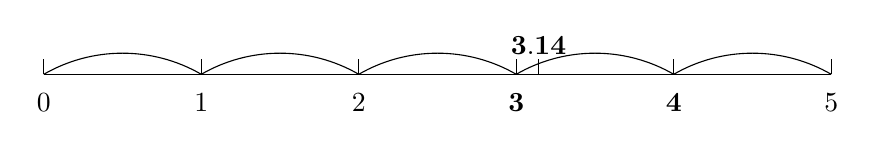
\begin{tikzpicture}[scale=2.0]
        \coordinate (O) at (0,0);
        \coordinate (I) at (1,0);
        \coordinate (II) at (2,0);
        \coordinate (III) at (3,0);
        \coordinate (IV) at (4,0);
        \coordinate (V) at (5,0);

        \coordinate (PI) at (3.1415926,0);

        \node [label={below:$0$}] at (O) {};
        \node [label={below:$1$}] at (I) {};
        \node [label={below:$2$}] at (II) {};
        \node [label={below:$\mathbf{3}$}] at (III) {};
        \node [label={above:$\mathbf{3.14}$}] at (PI) {};
        \node [label={below:$\mathbf{4}$}] at (IV) {};
        \node [label={below:$5$}] at (V) {};

        \draw (O) -- (I) -- (II) -- (III) -- (IV) -- (V);
        \draw (O) -- ++(0,0.1);
        \draw (I) -- ++(0,0.1);
        \draw (II) -- ++(0,0.1);
        \draw (III) -- ++(0,0.1);
        \draw (PI) -- ++(0,0.1);
        \draw (IV) -- ++(0,0.1);
        \draw (V) -- ++(0,0.1);

        \draw (O) arc (120:60:1);
        \draw (I) arc (120:60:1);
        \draw (II) arc (120:60:1);
        \draw (III) arc (120:60:1);
        \draw (IV) arc (120:60:1);
    \end{tikzpicture}
    \caption{Minh họa thuộc tính Archimedes với $x = 3.14$.}
\end{figure}

\begin{theorem}[Phần nguyên của số thực\index{Phần nguyên của số thực}]
    Với mọi số thực $x$, tồn tại duy nhất số nguyên $n$ sao cho $n\leq x < n+1$.

    \noindent Nói riêng, số nguyên $n$ như vậy được gọi là \textbf{phần nguyên của số thực $x$} và được kí hiệu là $\floor{x}$.
\end{theorem}

\begin{proof}
    Theo thuộc tính Archimedes, tồn tại số nguyên $a$ và $b$ sao cho $x < b$ và $-x < a$, kéo theo $-a < x < b$.

    Theo tính chất bắc cầu của quan hệ thứ tự trên tập hợp số thực, nếu một số nguyên $c$ thỏa mãn $c\leq x$ thì $c\leq b$. Theo nguyên lý thứ tự tốt, tập hợp các số nguyên nhỏ hơn hoặc bằng $x$ có phần tử lớn nhất, chúng ta kí hiệu phần tử đó là $n$. Vì $n < n + 1$ và $n + 1$ là một số nguyên nên theo định nghĩa của $n$, chúng ta có $n\leq x < n + 1$.

    Giả sử số nguyên $m$ thỏa mãn $m\leq x < m + 1$. Giả sử phản chứng rằng $m < n$, khi đó $m + 1\leq n$, kéo theo $m + 1\leq x$, mâu thuẫn với $x < m + 1$. Giả sử phản chứng rằng $n < m$, khi đó $n + 1\leq m$, kéo theo $n + 1\leq x$, mâu thuẫn với $x < n + 1$. Do đó $m = n$.

    Vậy với mọi số thực $x$, tồn tại duy nhất số nguyên $n$ sao cho $n\leq x < n+1$.
\end{proof}

\begin{theorem}[Tính trù mật của tập hợp số hữu tỉ\index{Tính trù mật của tập hợp số hữu tỉ}]
    Với mọi số thực $x, y$ sao cho $x < y$, tồn tại số hữu tỉ $q$ sao cho $x < q < y$.
\end{theorem}

\begin{proof}
    Theo thuộc tính Archimedes, tồn tại số nguyên $n$ sao cho $1 < n(y - x)$. Do đó $1 + nx < ny$. Theo định nghĩa phần nguyên của số thực, chúng ta có $nx < \floor{nx} + 1 \leq nx + 1 < ny$.

    Do đó, với số nguyên $m = \floor{nx} + 1$, chúng ta có $nx < m < ny$. Bên cạnh đó, vì $y - x > 0$ và $n > 0$ nên  $1 < n(y - x)$ kéo theo $n > 0$. Do đó $x < \frac{m}{n} < y$.

    Vậy, với mọi số thực $x, y$ sao cho $x < y$, tồn tại số hữu tỉ $q$ sao cho $x < q < y$.
\end{proof}

\subsection{* Sự tương đương của các mô hình số thực}

Chúng ta đã đưa ra hai mô hình số thực là lát cắt Dedekind và lớp tương đương của các dãy Cauchy hữu tỉ. Bên cạnh hai mô hình này, các nhà toán học còn đưa ra nhiều mô hình khác cho số thực. Điều này đặt ra câu hỏi rằng việc mỗi người chọn một mô hình khác nhau có gây ảnh hưởng gì không? Trong trường hợp của hệ tiên đề về số thực, các mô hình là ``tương đương'', như trong định lý sau đây.

Bạn đọc lưu ý rằng: với Định lý~\ref{theorem:embed-Q-into-the-set-of-dedekind-cuts}, chúng ta đồng nhất mỗi số hữu tỉ $q$ với lát cắt $q^{*} = \{ x \mid x\in\mathbb{Q} \wedge x < q \}$ (tập hợp các số hữu tỉ nhỏ hơn $q$).

\begin{theorem}\label{theorem:uniqueness-of-complete-ordered-field}
    Nếu tập hợp $R$ với phép cộng (${+}_{R}$) với phần tử đồng nhất của phép cộng ($0_{R}$), phép nhân (${\times}_{R}$) với phần tử đồng nhất của phép nhân ($1_{R}$), và quan hệ thứ tự ($\leq_{R}$) thỏa mãn hệ tiên đề về số thực thì tồn tại một song ánh $f: \mathscr{D}_{\mathbb{Q}}\to R$ sao cho
    \begin{itemize}[topsep=0pt,itemsep=0pt]
        \item $f(0) = 0_{R}$, $f(1) = 1_{R}$.
        \item $f(x + y) = f(x) +_{R} f(y)$ với mọi số thực $x, y$.
        \item $f(xy) = f(x) \times_{R} f(y)$ với mọi số thực $x, y$.
        \item $x\leq y$ kéo theo $f(x)\leq_{R} f(y)$ với mọi số thực $x, y$.
    \end{itemize}
\end{theorem}

Chứng minh dưới đây phỏng theo chứng minh trong cuốn sách Calculus của M.\@Spivak~\cite{spivak}. Chúng tôi chia chứng minh thành các bước nhỏ hơn để tiện theo dõi.

\begin{proof}
    Chúng ta định nghĩa ánh xạ $f: \mathscr{D}_{\mathbb{Q}}\to R$ như sau.

    \begin{enumerate}[label={\textbf{Bước \arabic*.}},itemindent=1cm]
        \item Định nghĩa ảnh của các số nguyên dưới ánh xạ $f$.

              Chúng ta gán $0$ với phần tử đồng nhất của phép cộng trong $R$, gán $1$ với phần tử đồng nhất của phép nhân trong $R$. Nói cách khác, $f(0) = 0_{R}$, $f(1) = 1_{R}$.

              Chúng ta gán các số nguyên dương và số nguyên âm với các phần tử của $R$ theo quy tắc: Nếu $n$ là một số nguyên dương thì $f(n) = f(n-1) + 1_{R}$, $f(-n) = -f(n)$.
        \item Chứng minh $f(m + n) = f(m) +_{R} f(n)$ với mọi số nguyên $m, n$.
              \begin{enumerate}[label={\textbf{Trường hợp \arabic*.}},itemindent=1.5cm]
                  \item Ít nhất một trong hai số nguyên $m$ hoặc $n$ là số nguyên không âm.

                        Không mất tính tổng quát, chúng ta giả sử $n$ là số nguyên không âm.

                        Khi $n = 0$, chúng ta có $f(m + n) = f(m) = f(m) +_{R} 0_{R}$.

                        Giả sử với số nguyên không âm $n = k$, chúng ta có $f(m + n) = f(m) +_{R} f(n)$. Khi đó, theo giả thiết quy nạp
                        \begin{align*}
                            f(m + (k+1)) & = f((m + k) + 1) = f(m + k) +_{R} 1_{R} \\
                                         & = (f(m) +_{R} f(k)) +_{R} 1_{R}         \\
                                         & = f(m) +_{R} (f(k) +_{R} 1_{R})         \\
                                         & = f(m) +_{R} f(k+1).
                        \end{align*}

                        Theo nguyên lý quy nạp toán học, với mọi số nguyên không âm $n$ và với mọi số nguyên $m$, chúng ta có $f(m + n) = f(m) + f(n)$.
                  \item $m$ hoặc $n$ là các số nguyên âm.

                        Theo \textbf{Trường hợp 1},
                        \begin{align*}
                            f(m + n) & = -f((-n) + (-m)) = -(f(-n) +_{R} f(-m)) \\
                                     & = (-f(-m)) +_{R} (-f(-n))                \\
                                     & = f(m) +_{R} f(n).
                        \end{align*}
              \end{enumerate}

              Do đó với mọi số nguyên $m, n$, chúng ta có $f(m + n) = f(m) +_{R} f(n)$.
        \item Chứng minh $f(mn) = f(m) \times_{R} f(n)$ với mọi số nguyên $m, n$.
              \begin{enumerate}[label={\textbf{Trường hợp \arabic*.}},itemindent=1.5cm]
                  \item Ít nhất một trong hai số nguyên $m$ hoặc $n$ là số nguyên không âm.

                        Không mất tính tổng quát, chúng ta giả sử $n$ là số nguyên không âm.

                        Khi $n = 0$, chúng ta có $f(mn) = f(0) = f(m)\times_{R} 0_{R} = f(m) \times_{R} f(n)$.

                        Giả sử với số nguyên không âm $n = k$, chúng ta có $f(mn) = f(m) \times_{R} f(n)$. Khi đó, theo giả thiết quy nạp
                        \begin{align*}
                            f(m(k+1)) & = f(mk + m) = f(mk) +_{R} f(m)               \\
                                      & = f(m)\times_{R} f(k) +_{R} f(m)\times 1_{R} \\
                                      & = f(m)\times_{R} (f(k) + 1_{R})              \\
                                      & = f(m)\times_{R} f(k+1)
                        \end{align*}

                        Theo nguyên lý quy nạp toán học, với mọi số nguyên không âm $n$ và với mọi số nguyên $m$, chúng ta có $f(mn) = f(m)\times_{R} f(n)$.
                  \item $m$ hoặc $n$ là các số nguyên âm.

                        Theo \textbf{Trường hợp 1},
                        \begin{align*}
                            f(mn) & = f((-m)(-n)) = f(-m)\times_{R} f(-n) \\
                                  & = (-f(-m))\times_{R} (-f(-n))         \\
                                  & = f(m) \times_{R} f(n).
                        \end{align*}
              \end{enumerate}

              Do đó với mọi số nguyên $m, n$, chúng ta có $f(m + n) = f(m) +_{R} f(n)$.

        \item Chứng minh $m\leq n$ kéo theo $f(m) \leq_{R} f(n)$ với mọi số nguyên $m, n$.

              Chúng ta chứng minh mệnh đề sau: Với mọi số nguyên dương $n$, $0_{R} <_{R} f(n)$.

              Với $n = 1$, chúng ta có $0_{R}\leq 1_{R}$ và $0_{R}\ne 1_{R}$ theo hệ tiên đề về số thực, do đó $0_{R} < 1_{R}$.

              Giả sử với số nguyên dương $n = k$, có $0_{R} < f(k)$. Khi đó, theo hệ tiên đề về số thực và giả thiết quy nạp, chúng ta có
              \[
                  0_{R}\leq 0_{R} +_{R} 1_{R}\leq f(k) +_{R} 1_{R} = f(k+1).
              \]

              Giả sử phản chứng rằng $f(k + 1) = 0_{R}$, khi đó $f(k) +_{R} 1_{R} = 0_{R}$, kéo theo $0_{R}\geq 1_{R} +_{R} + 0_{R} = 1_{R}$, dẫn đến $0_{R} = 1_{R}$ theo tính chất phản đối xứng. Do đó giả sử phản chứng là sai, điều này có nghĩa là $f(k+1)\ne 0_{R}$. Theo nguyên lý quy nạp toán học, với mọi số nguyên dương $n$, $0_{R} <_{R} f(n)$.

              Từ mệnh đề trên, cùng với hệ tiên đề về số thực, chúng ta suy ra
              \[
                  f(-n) = 0_{R} +_{R} f(-n) \leq_{R} f(n) +_{R} f(-n) = 0_{R}
              \]

              và $f(-n)\ne f(n) +_{R} f(-n)$, kéo theo $f(-n) \leq_{R} 0_{R}$ và $f(-n)\ne 0_{R}$.

              Với mọi số nguyên $m, n$, nếu $m\leq n$ thì tồn tại số nguyên không âm $k$ sao cho $m + k = n$. Theo \textbf{Bước 2}, chúng ta có $f(n) = f(m + k) = f(m) +_{R} f(k)$. Mặt khác, theo mệnh đề vừa chứng minh, chúng ta có $0_{R}\leq_{R} f(k)$, dẫn đến $f(m)\leq_{R} f(n)$.
        \item Định nghĩa ảnh của các số hữu tỉ dưới ánh xạ $f$.

              Theo chứng minh ở \textbf{Bước 4}, nếu số nguyên $n$ khác $0$ thì $f(n)\ne 0_{R}$. Do đó, nếu số nguyên $n$ khác $0$ thì $f(n)$ có nghịch đảo. Theo \textbf{Bước 3}, nếu $\dfrac{a}{b} = \dfrac{c}{d}$ thì $f(a)\times_{R} {(f(b))}^{-1} = f(c)\times_{R} {(f(d))}^{-1}$. Điều này là cơ sở để chúng ta định nghĩa ảnh của một số hữu tỉ $q = \dfrac{a}{b}$ dưới ánh xạ $f$ như sau
              \[
                  f(q) = f\left(\frac{a}{b}\right) = f(a)\times_{R} {(f(b))}^{-1}.
              \]
        \item Chứng minh $f(q_{1} + q_{2}) = f(q_{1}) +_{R} f(q_{2})$, $f(q_{1}q_{2}) = f(q_{1}) \times_{R} f(q_{2})$, $q_{1} < q_{2}\implies f(q_{1}) <_{R} f(q_{2})$ với mọi số hữu tỉ $q_{1}, q_{2}$.

              Chúng ta kí hiệu $\frac{a}{b}$ và $\frac{c}{d}$ lần lượt là các phân số tối giản của $q_{1}$ và $q_{2}$. Lưu ý rằng $b$ và $d$ là các số nguyên dương. Theo định nghĩa ảnh của số hữu tỉ dưới ánh xạ $f$
              \begingroup
              \allowdisplaybreaks
              \begin{align*}
                  f\left( \frac{a}{b} + \frac{c}{d} \right)   & = f\left( \frac{ad + bc}{bd} \right) = f(ad + bc)\times_{R} {(f(bd))}^{-1}                                                   \\
                                                              & = (f(ad) +_{R} f(bc)) \times_{R} {(f(bd))}^{-1}                                                                              \\
                                                              & = f(ad) \times_{R} {(f(bd))}^{-1} +_{R} f(bc) \times_{R} {(f(bd))}^{-1}                                                      \\
                                                              & = f\left(\frac{ad}{bd}\right) +_{R} f\left(\frac{bc}{bd}\right) = f\left(\frac{a}{b}\right) +_{R} f\left(\frac{c}{d}\right), \\
                  f\left( \frac{a}{b}\cdot\frac{c}{d} \right) & = f\left(\frac{ac}{bd}\right) = f(ac)\times_{R} {(f(bd))}^{-1}                                                               \\
                                                              & = (f(a)\times_{R} f(c)) \times_{R} ({(f(d))}^{-1}\times_{R} {(f(c))}^{-1})                                                   \\
                                                              & = (f(a)\times_{R} {(f(b))}^{-1}) \times_{R} (f(c)\times_{R} {(f(d))}^{-1})                                                   \\
                                                              & = f\left(\frac{a}{b}\right)\times_{R} f\left(\frac{c}{d}\right).
              \end{align*}
              \endgroup

              Nếu $\frac{a}{b} < \frac{c}{d}$ thì $ad < bc$. Theo \textbf{Bước 4}, $f(ad) <_{R} f(bc)$. Mặt khác, $f(ad) = f(a)\times_{R} f(d)$, $f(bc) = f(b) \times_{R} f(c)$. Do đó $f(a)\times_{R} f(d) <_{R} f(b)\times_{R} f(c)$ và kéo theo
              \[
                  f(a)\times_{R} f(d) <_{R} f(b)\times_{R} f(c).
              \]

              Bên cạnh đó, $0_{R} <_{R} f(c), 0_{R} <_{R} f(d)$ vì $c, d$ là các số nguyên dương, nên $0_{R} < {(f(c))}^{-1}, 0_{R} <_{R} {(f(d))}^{-1}$ và chúng ta suy ra
              \[
                  f(a)\times_{R} {(f(b))}^{-1} <_{R} f(c)\times_{R} {(f(d))}^{-1}.
              \]

              Do đó $f\left(\dfrac{a}{b}\right) <_{R} f\left(\dfrac{c}{d}\right)$.
        \item Định nghĩa ảnh của các số thực dưới ánh xạ $f$.

              Với mỗi số thực $x$, chúng ta kí hiệu $S_{x}$ là tập hợp tất cả các số hữu tỉ nhỏ hơn $x$. Tập hợp $S_{x}$ là một lát cắt trên tập hợp các số hữu tỉ (do đó, $x = S_{x}$), vì
              \begin{enumerate}[label={(DC\arabic*)},itemindent=0.5cm]
                  \item $S_{x}$ không rỗng, $\mathbb{Q}\setminus S_{x}$ không rỗng.
                  \item Mọi phần tử của $S_{x}$ nhỏ hơn mọi phần tử của $\mathbb{Q}\setminus S_{x}$, theo tính chất bắc cầu của quan hệ thứ tự trên tập hợp số hữu tỉ.
                  \item Với mỗi số hữu tỉ $a$ thuộc $S_{x}$, luôn tồn tại một số hữu tỉ khác lớn hơn $a$ và cũng thuộc $S_{x}$, điều này được suy ra từ việc áp dụng tính trù mật của tập hợp số hữu tỉ cho hai số thực $a$ và $x$. Do đó $S_{x}$ không có phần tử lớn nhất.
                  \item Nếu số hữu tỉ $a$ thuộc $S_{x}$ thì mọi số hữu tỉ nhỏ hơn $a$ cũng thuộc $S_{x}$, theo tính chất bắc cầu của quan hệ thứ tự trên tập hợp số hữu tỉ.
              \end{enumerate}

              Bên cạnh đó, $x$ là cận trên nhỏ nhất của $S_{x}$. Bởi vì với mọi số thực $y < x$, luôn tồn tại số hữu tỉ $q$ sao cho $y < q < x$, đồng nghĩa với việc mọi số thực nhỏ hơn $x$ đều không phải cận trên của $S_{x}$.

              Vì $S_{x}$ có cận trên nên theo kết quả ở \textbf{Bước 6}, ảnh của $S_{x}$ dưới ánh xạ $f$ (được kí hiệu là $f[S_{x}]$) cũng có cận trên. Theo tiên đề về cận trên, $f[S_{x}]$ có cận trên nhỏ nhất.

              Để định nghĩa ảnh của số thực dưới ánh xạ $f$ tương thích với định nghĩa ảnh của số hữu tỉ dưới ánh xạ $f$, chúng ta cần chỉ ra rằng khi $x$ là một số hữu tỉ thì $\sup f[S_{x}] = f(x)$. Với mọi số hữu tỉ $q$ nhỏ hơn $x$, chúng ta có $f(q) <_{R} f(x)$. Do đó, $\sup f[S_{x}]\leq_{R} f(x)$. Giả sử phản chứng rằng $\sup f[S_{x}] <_{R} f(x)$. Theo tính trù mật của tập hợp số hữu tỉ\footnote{Để hiểu vì sao có thể sử dụng tính trù mật của tập hợp số hữu tỉ, bạn đọc hãy nhìn nhận $f(n)$ như số nguyên trong $R$ (trong đó $n$ là số nguyên) và nhìn nhận $f(q)$ như số hữu tỉ trong $R$ (trong đó $q$ là số hữu tỉ).}, giữa hai phần tử $\sup f[S_{x}]$ và $f(x)$, tồn tại số hữu tỉ $q'$ sao cho $\sup f[S_{x}] <_{R} f(q') <_{R} f(x)$. Vì $f(q') <_{R} f(x)$ và $x$, $q'$ là các số hữu tỉ nên theo \textbf{Bước 6}, chúng ta có $q < q' < x$. Do đó $q'$ thuộc $S_{x}$ và $f(q')$ thuộc $f[S_{x}]$, mâu thuẫn với $\sup f[S_{x}] <_{R} f(q')$. Như vậy giả sử phản chứng là sai, kéo theo $\sup f[S_{x}] = f(x)$ khi $x$ là số hữu tỉ.

              Chúng ta định nghĩa ảnh của số thực $x$ dưới ánh xạ $f$ là $\sup f[S_{x}]$.
    \end{enumerate}

    Như vậy chúng ta đã định nghĩa một ánh xạ $f: \mathscr{D}_{\mathbb{Q}}\to R$.
    \begin{enumerate}[label={\textbf{Bước \arabic*.}},itemindent=1cm,start=8]
        \item Chứng minh rằng với mọi số thực $x, y$, $x\leq y$ kéo theo $f(x) \leq_{R} f(y)$.

              Nếu $x = y$ thì $f(x) = f(y)$.

              Nếu $x < y$ thì theo tính trù mật của tập hợp số hữu tỉ, tồn tại các số hữu tỉ $q, q'$ sao cho $x < q < q' < y$. Vì $x$ là cận trên nhỏ nhất của $S_{x}$ và $x < q$ nên $f(x)\leq_{R} f(q)$. Với hai số hữu tỉ $q < q'$, chúng ta có $f(q) <_{R} f(q')$, do đó $f(x) <_{R} f(q')$. Bên cạnh đó, $q'$ thuộc $S_{y}$ nên $f(q')\leq_{R} f(y)$. Do đó $f(x) <_{R} f(y)$.

              Như vậy, $x\leq y$ kéo theo $f(x) \leq_{R} f(y)$.
        \item Chứng minh rằng với mọi số thực $x, y$, có $f(x + y) = f(x) +_{R} f(y)$.

              Giả sử phản chứng rằng $f(x + y) <_{R} f(x) +_{R} f(y)$. Theo tính trù mật của tập hợp số hữu tỉ, tồn tại số hữu tỉ $q$ sao cho $f(x + y) <_{R} f(q) <_{R} f(x) +_{R} f(y)$. Theo \textbf{Bước 8}, chúng ta có $x + y < q$. Theo tính trù mật của tập hợp số hữu tỉ, tồn tại số hữu tỉ $a$ sao cho $x < a < q - y$, và tồn tại số hữu tỉ $b$ sao cho $y < b < q - a$. Do đó, $x + y < a + b < q$. Theo \textbf{Bước 8}, chúng ta có $f(x) <_{R} f(a)$ và $f(y) <_{R} f(b)$. Theo \textbf{Bước 6}, $f(x) +_{R} f(y) <_{R} f(a) +_{R} f(b) = f(a + b) <_{R} f(q)$, điều này mâu thuẫn với $f(q) <_{R} f(x) +_{R} f(y)$.

              Giả sử phản chứng rằng $f(x + y) >_{R} f(x) +_{R} f(y)$. Chúng ta chứng minh tương tự. Theo tính trù mật của tập hợp số hữu tỉ, tồn tại số hữu tỉ $q$ sao cho $f(x) +_{R} f(y) <_{R} f(q) <_{R} f(x+y)$. Theo \textbf{Bước 8}, chúng ta có $q < x + y$. Theo tính trù mật của tập hợp số hữu tỉ, tồn tại số hữu tỉ $a$ sao cho $q - y < a < x$, và tồn tại số hữu tỉ $b$ sao cho $q - a < b < y$. Do đó $x + y > a + b > q$.  Theo \textbf{Bước 8}, chúng ta có $f(x) >_{R} f(a)$ và $f(y) >_{R} f(b)$. Theo \textbf{Bước 6}, $f(x) +_{R} f(y) >_{R} f(a) +_{R} f(b) = f(a + b) >_{R} f(q)$, điều này mâu thuẫn với $f(q) >_{R} f(x) +_{R} f(y)$.

              Vậy các giả sử phản chứng là sai, kéo theo $f(x + y) = f(x) +_{R} f(y)$ (vì $\leq_{R}$ là một quan hệ thứ tự toàn phần trong $R$).

              Hệ quả của điều này là $f(-x) = -f(x)$, với mọi số thực $x$.
        \item Chứng minh rằng với mọi số thực $x, y$, có $f(xy) = f(x) \times_{R} f(y)$.

              Chúng ta xét đủ các trường hợp sau.
              \begin{enumerate}[label={\textbf{Trường hợp \arabic*.}},itemindent=2cm]
                  \item $x = 0$ hoặc $y = 0$.

                        $x = 0$ hoặc $y = 0$ thì $f(x) = 0_{R}$ hoặc $f(y) = 0_{R}$.

                        $f(xy) = f(0) = 0_{R} = f(x)\times_{R} f(y)$.
                  \item $x > 0$ và $y > 0$.

                        $x > 0$ và $y > 0$ thì $xy > 0$. Theo \textbf{Bước 8}, $0_{R} <_{R} f(x), f(y), f(xy)$, kéo theo $0_{R} <_{R} f(x)\times_{R} f(y)$.

                        Giả sử phản chứng rằng $f(xy) <_{R} f(x)\times_{R} f(y)$. Theo tính trù mật của tập hợp số hữu tỉ, tồn tại số hữu tỉ $q$ sao cho $f(xy) <_{R} f(q) <_{R} f(x)\times_{R} f(y)$. Theo \textbf{Bước 8}, chúng ta có $0 < xy < q$. Theo tính trù mật của tập hợp số hữu tỉ, tồn tại số hữu tỉ $a$ sao cho $x < a < \dfrac{q}{y}$, và tồn tại số hữu tỉ $b$ sao cho $y < b < \dfrac{q}{a}$. Do đó $xy < ab < q$. Theo \textbf{Bước 6}, $f(x)\times_{R} f(y) <_{R} f(a)\times_{R} f(b) = f(ab) <_{R} f(q)$, điều này mâu thuẫn với $ f(q) <_{R} f(x)\times_{R} f(y)$.

                        Giả sử phản chứng rằng $f(x)\times_{R} f(y) <_{R} f(xy)$. Theo tính trù mật của tập hợp số hữu tỉ, tồn tại số hữu tỉ $q$ sao cho $f(x)\times_{R} f(y) <_{R} f(q) <_{R} f(xy)$. Theo \textbf{Bước 8}, chúng ta có $0 < q < xy$. Theo tính trù mật của tập hợp số hữu tỉ, tồn tại số hữu tỉ $a$ sao cho $\dfrac{q}{y} < a < x$, và tồn tại số hữu tỉ $b$ sao cho $\dfrac{q}{a} < b < y$. Do đó $q < ab < xy$. Theo \textbf{Bước 6}, $f(x)\times_{R} f(y) >_{R} f(a)\times_{R} f(b) = f(ab) >_{R} f(q)$, điều này mâu thuẫn với $f(x)\times_{R} f(y) <_{R} f(q)$.

                        Vậy các giả sử phản chứng là sai, kéo theo $f(xy) = f(x) \times_{R} f(y)$ với mọi $x, y$ thỏa mãn $x > 0$ và $y > 0$ (vì $\leq_{R}$ là một quan hệ thứ tự toàn phần trong $R$).
                  \item $x > 0$ và $y < 0$.

                        Theo \textbf{Trường hợp 2}, \textbf{Bước 9} và Định lý~\ref{theorem:field-properties}, chúng ta có
                        \begin{align*}
                            f(xy) & = f(-x(-y)) = -f(x(-y))   \\
                                  & = -f(x)\times_{R} f(-y)   \\
                                  & = f(x)\times_{R} (-f(-y)) \\
                                  & = f(x)\times_{R} f(y).
                        \end{align*}
                  \item $x < 0$ và $y > 0$.
                        Theo \textbf{Trường hợp 2}, \textbf{Bước 9} và Định lý~\ref{theorem:field-properties}, chúng ta có
                        \begin{align*}
                            f(xy) & = f(-(-x)y) = -f((-x)y)   \\
                                  & = -f(-x)\times_{R} f(y)   \\
                                  & = (-f(-x))\times_{R} f(y) \\
                                  & = f(x)\times_{R} f(y).
                        \end{align*}
                  \item $x < 0$ và $y > 0$.
                        Theo \textbf{Trường hợp 2}, \textbf{Bước 9} và Định lý~\ref{theorem:field-properties}, chúng ta có
                        \begin{align*}
                            f(xy) & = f((-x)(-y))                 \\
                                  & = f(-x)\times_{R} f(-y)       \\
                                  & = (-f(-x))\times_{R} (-f(-y)) \\
                                  & = f(x)\times_{R} f(y).
                        \end{align*}
              \end{enumerate}

              Vậy $f(xy) = f(x)\times_{R} f(y)$ với mọi số thực $x, y$.
        \item Chứng minh $f$ là song ánh.

              Giả sử $f(x) = f(y)$. Theo \textbf{Bước 8}, nếu $x < y$ thì $f(x) <_{R} f(y)$ và nếu $y < x$ thì $f(y) <_{R} f(x)$. Do đó $x = y$. Như vậy $f$ là một đơn ánh.

              Giả sử $a$ là một phần tử của $R$. Trong $R$, tồn tại phần tử $b$, $c$ sao cho $b <_{R} a <_{R} c$. Theo tính trù mật của tập hợp số hữu tỉ, tồn tại các số hữu tỉ $q$ và $q'$ sao cho $b <_{R} f(q) <_{R} a$ và $a <_{R} f(q') <_{R} c$. Như vậy tập hợp $S$ gồm tất cả các số hữu tỉ $r$ sao cho $f(r) < a$ không rỗng và bị chặn trên. Theo tiên đề về cận trên, $S$ có cận trên nhỏ nhất, chúng ta kí hiệu $x = \sup S$.

              Giả sử phản chứng rằng $f(x) <_{R} a$. Theo tính trù mật của tập hợp số hữu tỉ, tồn tại các số hữu tỉ $q$ sao cho $f(x) <_{R} f(q) <_{R} a$. Theo \textbf{Bước 8}, $\sup S = x < q$, điều này mâu thuẫn với việc $q$ là một phần tử của $S$.

              Giả sử phản chứng rằng $a <_{R} f(x)$. Theo tính trù mật của tập hợp số hữu tỉ, tồn tại các số hữu tỉ $q$ sao cho $a <_{R} f(q) <_{R} f(x)$. Theo \textbf{Bước 8}, $q < x = \sup S$, kéo theo $q$ thuộc $S$. Vì $q$ thuộc $S$ nên $f(q) <_{R} a$, điều này mâu thuẫn với việc $a <_{R} f(q)$.

              Do đó các giả sử phản chứng là sai, kéo theo $f(x) = a$ (vì $\leq_{R}$ là một quan hệ thứ tự toàn phần trong $R$). Như vậy $f$ là một toàn ánh.

              Vì $f$ vừa là một đơn ánh, vừa là một toàn ánh nên $f$ cũng là một song ánh.
    \end{enumerate}

    Vậy $\mathscr{D}_{\mathbb{Q}}$ và $R$ đẳng cấu.
\end{proof}

Trong Định lý~\ref{theorem:uniqueness-of-complete-ordered-field}, $f$ được gọi là một đẳng cấu trường bảo toàn thứ tự. Với định lý này, chúng ta kết luận rằng mọi mô hình số thực đẳng cấu, hay tập hợp số thực là duy nhất, sai khác một đẳng cấu.

\begin{theorem}
    Mọi mô hình số thực là đẳng cấu với nhau.
\end{theorem}

Tập hợp số thực còn được gọi là \textbf{trường số thực\index{Trường số thực}}, hay \textbf{trường được sắp thứ tự đầy đủ\index{Trường được sắp thứ tự đầy đủ}} (tên gọi trường, sắp thứ tự, và đầy đủ tương ứng với ba nhóm tiên đề trong hệ tiên đề về số thực). Chúng ta có thể sử dụng hệ tiên đề số thực hay bất kì mô hình số thực nào để định nghĩa số thực, giống như có thể sử dụng bất kì phần tử nào của một lớp tương đương để làm phần tử đại diện của lớp tương đương đó.

\subsection{Nhìn nhận về các tập hợp số}

% pending

\section{Nhập môn giải tích thực}

Giải tích thực là một ngành toán học nghiên cứu về các hàm số thực, lý thuyết hàm thực cũng là tên gọi trước đây của giải tích thực. Một giáo trình mẫu mực về giải tích thực luôn có các nội dung sau: số thực, giới hạn của dãy số, chuỗi số, giới hạn của hàm số, tính liên tục, vi phân, tích phân. Tuy nhiên, trong thực tế giảng dạy ở chương trình phổ thông cũng như đại học, phần nhiều vì thường không có đủ thời gian nên những nội dung cơ bản hơn (số thực, giới hạn của dãy số, giới hạn của hàm số, tính liên tục) không được đào sâu vào chi tiết, không tuân theo trình tự chặt chẽ, và thừa nhận những định nghĩa, tính chất của hàm lũy thừa, hàm mũ, hàm logarithm. Trong mục này, chúng ta sẽ triển khai nội dung về giới hạn của dãy số, giới hạn của hàm số, tính liên tục, cùng hàm lũy thừa, hàm mũ, hàm logarithm.

\subsection{Dãy số thực và giới hạn}

Kết quả chính của mục này là tính đầy đủ-Cauchy --- Mọi dãy Cauchy đều hội tụ.

\begin{definition}[Giá trị tuyệt đối của số thực]
    Ánh xạ $\abs{\cdot}: \mathbb{R}\to \mathbb{R}_{\geq 0}$ được định nghĩa bởi
    \[
        \abs{x} = \begin{cases}
            x  & \text{nếu $x\geq 0$}, \\
            -x & \text{nếu $x < 0$}
        \end{cases}
    \]

    được gọi là \textbf{ánh xạ giá trị tuyệt đối}, hay \textbf{hàm giá trị tuyệt đối} của số thực\index{Giá trị tuyệt đối của số thực}. Số thực không âm $\abs{x}$ được gọi là giá trị tuyệt đối của số thực $x$.
\end{definition}

Trong Mục~\ref{section:rational-cauchy-sequences}, khi chuẩn bị cho việc xây dựng mô hình số thực bằng dãy Cauchy hữu tỉ, chúng ta đã đưa ra khái niệm dãy số hữu tỉ và một số định nghĩa liên quan. Dưới đây, chúng ta đưa ra các định nghĩa tương tự và dành cho dãy số thực (chỉ thay số hữu tỉ thành số thực).

\begin{definition}[Dãy số thực]
    Ánh xạ $f: \mathbb{N}\to \mathbb{R}$ được gọi là một \textbf{dãy số thực\index{Dãy số thực}}, hay \textbf{dãy số}, \textbf{dãy} (trong ngữ cảnh giải tích thực).
    \begin{enumerate}[label={(\roman*)}]
        \item Dãy ${(f_{n})}_{n\in\mathbb{N}}$ được gọi là \textbf{dãy hằng số\index{Dãy hằng số}} nếu và chỉ nếu giá trị tại mọi chỉ số $n$ của dãy này là như nhau.
        \item Dãy ${(f_{n})}_{n\in\mathbb{N}}$ được gọi là \textbf{dãy dừng\index{Dãy dừng}} nếu và chỉ nếu tồn tại số tự nhiên $n_{0}$ sao cho giá trị tại mọi chỉ số $n\geq n_{0}$ là như nhau.
        \item Dãy ${(f_{n})}_{n\in\mathbb{N}}$ được gọi là \textbf{dãy tăng\index{Dãy tăng}}, hay \textbf{dãy tăng thực sự} nếu và chỉ nếu tồn tại số tự nhiên $n_{0}$ sao cho $f_{n+1} > f_{n}$ với mọi số tự nhiên $n\geq n_{0}$.
        \item Dãy ${(f_{n})}_{n\in\mathbb{N}}$ được gọi là \textbf{dãy giảm\index{Dãy giảm}}, hay \textbf{dãy giảm thực sự} nếu và chỉ nếu tồn tại số tự nhiên $n_{0}$ sao cho $f_{n+1} < f_{n}$ với mọi số tự nhiên $n\geq n_{0}$.
        \item Dãy ${(f_{n})}_{n\in\mathbb{N}}$ được gọi là \textbf{dãy không giảm\index{Dãy không giảm}} nếu và chỉ nếu tồn tại số tự nhiên $n_{0}$ sao cho $f_{n+1}\geq f_{n}$ với mọi số tự nhiên $n\geq n_{0}$.
        \item Dãy ${(f_{n})}_{n\in\mathbb{N}}$ được gọi là \textbf{dãy không tăng\index{Dãy không tăng}} nếu và chỉ nếu tồn tại số tự nhiên $n_{0}$ sao cho $f_{n+1}\leq f_{n}$ với mọi số tự nhiên $n\geq n_{0}$.
        \item Dãy ${(f_{n})}_{n\in\mathbb{N}}$ được gọi là \textbf{dãy bị chặn\index{Dãy bị chặn}} nếu và chỉ nếu tồn tại số thực $A$ sao cho với mọi số tự nhiên $n$, có $\abs{f_{n}}\leq A$ (hoặc $\abs{f_{n}} < A$).
        \item Dãy ${(f_{n})}_{n\in\mathbb{N}}$ được gọi là \textbf{dãy Cauchy\index{Dãy Cauchy thục}} nếu và chỉ nếu với mọi số thực dương $\varepsilon$, tồn tại số tự nhiên $N(\varepsilon)$ sao cho với mọi số tự nhiên $n, m\geq N(\varepsilon)$, có $\abs{f_{m} - f_{n}} < \varepsilon$. Bằng logic hình thức, chúng ta viết
              \[
                  \forall \varepsilon > 0\ \exists N(\varepsilon)\ \forall n, m\geq N(\varepsilon)\ \abs{f_{n} - f_{m}} < \varepsilon.
              \]
        \item Dãy ${(f_{n})}_{n\in\mathbb{N}}$ được gọi là hội tụ đến số thực $a$ nếu và chỉ nếu với mọi số thực dương $\varepsilon$, tồn tại số tự nhiên $N(\varepsilon)$ sao cho với mọi số tự nhiên $n\geq N(\varepsilon)$, có $\abs{f_{n} - a} < \varepsilon$. Bằng logic hình thức, chúng ta viết
              \[
                  \forall \varepsilon > 0\ \exists N(\varepsilon)\ \forall n\geq N(\varepsilon)\ \abs{f_{n} - a} < \varepsilon.
              \]
        \item Nếu tồn tại số thực $a$ sao cho dãy ${(f_{n})}_{n\in\mathbb{N}}$ hội tụ đến $a$ thì $a$ được gọi là một điểm giới hạn (hay giới hạn) của  dãy ${(f_{n})}_{n\in\mathbb{N}}$ và chúng ta nói dãy ${(f_{n})}_{n\in\mathbb{N}}$ hội tụ.
    \end{enumerate}
\end{definition}

Tương tự với dãy số hữu tỉ, chúng ta có các kết quả sau, với chứng minh hoàn toàn tương tự.
\begin{theorem}
    Dãy Cauchy là dãy bị chặn.
\end{theorem}

\begin{theorem}
    Nếu một dãy hội tụ thì điểm giới hạn của dãy đó là duy nhất.
\end{theorem}

Để biểu thị số thực $a$ là giới hạn của dãy ${(f_{n})}_{n\in\mathbb{N}}$, chúng ta kí hiệu $\lim f_{n} = a$.

\begin{theorem}\label{theorem:limits-of-sum-and-product-of-sequences}
    Nếu $\lim a_{n} = a$ và $\lim b_{n} = b$ thì
    \begin{enumerate}[label={(\roman*)}]
        \item $\lim (a_{n} + b_{n}) = a + b$.
        \item $\lim (a_{n}b_{n}) = ab$.
    \end{enumerate}
\end{theorem}

Với các định lý dưới đây, sự khác biệt (tiên đề về cận trên, hay tiên đề về tính đầy đủ) giữa tập hợp số thực và tập hợp số hữu tỉ được nhấn mạnh thêm nhiều lần.

\begin{theorem}[Định lý về dãy đơn điệu và bị chặn]
    Dãy đơn điệu không giảm và bị chặn trên thì hội tụ. Dãy đơn điệu không tăng và bị chặn dưới thì hội tụ\footnote{Định lý này còn có phát biểu ngắn gọn hơn: Dãy đơn điệu và bị chặn thì hội tụ.}.
\end{theorem}

\begin{proof}
    \begin{enumerate}[label={(\roman*)}]
        \item Giả sử dãy ${(a_{n})}_{n\in\mathbb{N}}$ không giảm và bị chặn. Như vậy tập hợp tất cả các giá trị của dãy ${(a_{n})}_{n\in\mathbb{N}}$ là khác rỗng và bị chặn trên. Theo tiên đề về cận trên, tập hợp tất cả các giá trị của dãy ${(a_{n})}_{n\in\mathbb{N}}$ có cận trên nhỏ nhất. Chúng ta kí hiệu cận trên nhỏ nhất này là $a$.

              Dãy ${(a_{n})}_{n\in\mathbb{N}}$ không giảm nên tồn tại số tự nhiên $n_{0}$ sao cho $a_{n+1}\geq a_{n}$ với mọi $n\geq n_{0}$.

              Theo định nghĩa cận trên nhỏ nhất, với mọi số thực dương $\varepsilon$, $a - \varepsilon$ không phải cận trên của tập hợp tất cả các giá trị của dãy ${(a_{n})}_{n\in\mathbb{N}}$. Do đó, với mỗi số thực dương $\varepsilon$, tồn tại số tự nhiên $n_{1}$ sao cho $a_{n_{1}} > a - \varepsilon$. Vì dãy ${(a_{n})}_{n\in\mathbb{N}}$ không giảm nên $a - a_{n}\leq a - a_{n_{1}} < \varepsilon$ với mọi số tự nhiên $n\geq N = \max\{ n_{0}, n_{1} \}$. Bên cạnh đó, $\abs{a - a_{n}} = a - a_{n}$ với mọi số tự nhiên $n$ vì $a$ là cận trên nhỏ nhất của tập hợp tất cả các giá trị của dãy ${(a_{n})}_{n\in\mathbb{N}}$.

              Như vậy, với mỗi số thực dương $\varepsilon$, tồn tại số tự nhiên $N$ sao cho với mọi số tự nhiên $n\geq N$, có $\abs{a_{n} - a} < \varepsilon$. Do đó, dãy ${(a_{n})}_{n\in\mathbb{N}}$ hội tụ.
        \item Giả sử dãy ${(a_{n})}_{n\in\mathbb{N}}$ không tăng và bị chặn. Khi đó dãy $(b_{n})_{n\in\mathbb{N}}$ được định nghĩa bởi $b_{n} = -a_{n}$ với mọi số tự nhiên $n$ là một dãy không giảm và bị chặn. Theo phần (i), dãy $(b_{n})_{n\in\mathbb{N}}$ hội tụ. Theo Định lý~\ref{theorem:limits-of-sum-and-product-of-sequences}, dãy ${(a_{n})}_{n\in\mathbb{N}}$ hội tụ.
    \end{enumerate}
\end{proof}

Trong phần (ii) của chứng minh trên, thay vì áp dụng phần (i), chúng ta có thể chứng minh tương tự phần (i) bằng cách chỉ ra giới hạn của dãy số là cận dưới lớn nhất của tập hợp tất cả các giá trị của dãy ${(a_{n})}_{n\in\mathbb{N}}$.

\begin{definition}
    Cho hai số thực $a, b$ thỏa mãn $a\leq b$. Chúng ta định nghĩa \textbf{khoảng mở\index{Khoảng mở}} $(a, b)$ và \textbf{khoảng đóng\index{Khoảng đóng}} $[a, b]$ là hai tập hợp sau.
    \[
        \begin{split}
            (a, b) = \{ x\in\mathbb{R} \mid a < x < b \}, \\
            [a, b] = \{ x\in\mathbb{R} \mid a\leq x\leq b \}.
        \end{split}
    \]
\end{definition}

Nói riêng, nếu hai số thực $a, b$ thỏa mãn $a = b$ thì $(a, b) = \varnothing$ và $[a, b] = \{ a \}$.

\begin{theorem}[Định lý Cantor về các khoảng đóng lồng nhau]
    Hai dãy số ${(a_{n})}_{n\in\mathbb{N}}$ và ${(b_{n})}_{n\in\mathbb{N}}$ thỏa mãn $a_{n}\leq b_{n}$, $[a_{n+1}, b_{n+1}]\subseteq [a_{n}, b_{n}]$ với mọi số tự nhiên $n$.
    \begin{enumerate}[label={(\roman*)}]
        \item $\bigcap_{n\in\mathbb{N}} [a_{n}, b_{n}]\ne \varnothing$.
        \item Nếu $\lim (a_{n} - b_{n}) = 0$ thì tập hợp $\bigcap_{n\in\mathbb{N}} [a_{n}, b_{n}]$ có đúng một phần tử.
    \end{enumerate}
\end{theorem}

\begin{proof}
    \begin{enumerate}[label={(\roman*)}]
        \item Vì $[a_{n+1}, b_{n+1}]\subseteq [a_{n}, b_{n}]$ với mọi số tự nhiên $n$ nên $a_{n}\leq a_{n+1}$ và $b_{n}\geq b_{n+1}$ với mọi số tự nhiên $n$. Vì $a_{n}\leq a_{n+1}$ và $b_{n}\geq b_{n+1}$ với mọi số tự nhiên $n$ nên $a_{0}\leq a_{n}$ và $b_{n}\leq b_{0}$ với mọi số tự nhiên $n$ (điều này được chứng minh bằng phương pháp quy nạp toán học). Vì $a_{n}\leq b_{n}$ với mọi số tự nhiên $n$ nên $a_{n}\leq b_{n}\leq b_{0}$ và $a_{0}\leq a_{n}\leq b_{n}$ với mọi số tự nhiên $n$. Do đó dãy số ${(a_{n})}_{n\in\mathbb{N}}$ bị chặn trên, dãy số ${(b_{n})}_{n\in\mathbb{N}}$ bị chặn dưới. Kí hiệu $a = \sup {\{ a_{n}\}}_{n\in\mathbb{N}}$ và $b = \inf {\{ b_{n} \}}_{n\in\mathbb{N}}$. Giả sử phản chứng rằng $a > b$, khi đó $b$ không phải cận trên nhỏ nhất của ${\{ a_{n} \}}_{n\in\mathbb{N}}$, kéo theo tồn tại số tự nhiên $m$ sao cho $a_{m} > b$. Mà $b_{0}\leq b$ nên chúng ta suy ra $b_{0} < a_{m}$, điều này mâu thuẫn với mệnh đề vừa chứng minh ``$a_{n}\leq b_{0}$ với mọi số tự nhiên $n$''. Do đó, $a\leq b$. Chọn một phần tử $x$ bất kì từ khoảng đóng $[a, b]$, chúng ta có $a_{n}\leq a\leq x\leq b\leq b_{n}$ với mọi số tự nhiên $n$. Do đó, $x$ thuộc $\bigcap_{n\in\mathbb{N}} [a_{n}, b_{n}]$. Như vậy $\bigcap_{n\in\mathbb{N}} [a_{n}, b_{n}]\ne\varnothing$.
        \item Với các giá trị $a, b$ ở phần (i), chúng ta chứng minh rằng
              \[
                  \bigcap_{n\in\mathbb{N}} [a_{n}, b_{n}] = [a, b].
              \]

              Giả sử $x$ thuộc $[a, b]$ thì $x$ thuộc $[a_{n}, b_{n}]$ với mọi số tự nhiên $n$ vì $a_{n}\leq a$ và $b\leq b_{n}$ với mọi số tự nhiên $n$. Do đó $x$ thuộc $[a_{n}, b_{n}]$ với mọi số tự nhiên $n$, kéo theo $x$ thuộc $\bigcap_{n\in\mathbb{N}} [a_{n}, b_{n}]$. Như vậy $[a, b]\subseteq \bigcap_{n\in\mathbb{N}} [a_{n}, b_{n}]$.

              Giả sử $x$ thuộc $\bigcap_{n\in\mathbb{N}} [a_{n}, b_{n}]$ (chúng ta giả sử được như vậy vì $\bigcap_{n\in\mathbb{N}} [a_{n}, b_{n}]\ne \varnothing$). Theo định nghĩa khoảng đóng, $a_{n}\leq x\leq b_{n}$ với mọi số tự nhiên $n$. Do đó $x$ là cận trên của ${\{a_{n}\}}_{n\in\mathbb{N}}$ và là cận dưới của ${\{b_{n}\}}_{n\in\mathbb{N}}$, kéo theo $a\leq x\leq b$, hay $x$ thuộc $[a, b]$. Như vậy $\bigcap_{n\in\mathbb{N}} [a_{n}, b_{n}]\subseteq [a, b]$.

              Vậy $\bigcap_{n\in\mathbb{N}} [a_{n}, b_{n}] = [a, b]$. Nếu $\lim (a_{n} - b_{n}) = 0$ thì $a = b$, kéo theo $[a, b]$ có đúng một phàn tử, do đó $\bigcap_{n\in\mathbb{N}} [a_{n}, b_{n}]$ có đúng một phần tử.
    \end{enumerate}
\end{proof}

Nói chung, định lý trên sẽ không còn đúng nếu chúng ta thay khoảng đóng bởi khoảng mở. Điều này sẽ được làm rõ hơn trong bài tập.

\begin{theorem}[Định lý Bolzano-Weierstra{\ss} cho số thực]
    Mọi dãy bị chặn đều chứa một dãy con\index{Dãy con} hội tụ.
\end{theorem}

Trước tiên, chúng ta làm rõ hơn khái niệm dãy con. Với một dãy ${(f_{n})}_{n\in\mathbb{N}}$, chúng ta lần lượt chọn vô hạn các số tự nhiên $n_{k}$ (trong đó $k\in\mathbb{N}$) sao cho $n_{0} < n_{1} < n_{2} < \cdots$ thì ${(f_{n_{k}})}_{k\in\mathbb{N}}$ là một dãy con của ${(f_{n})}_{n\in\mathbb{N}}$.
\begin{figure}[htp]
    \centering
    \begin{tikzpicture}
        \foreach \x in {0,...,12} {
                \node [label={below:$f_{\x}$}] at (\x, 0) {};
            }

        \node [label={below:$\longrightarrow$}] at (13, -0.6) {};

        \node [label={below:$f_{n_{0}}$}] at (2, -1) {};
        \node [label={below:$f_{n_{1}}$}] at (3, -1) {};
        \node [label={below:$f_{n_{2}}$}] at (5, -1) {};
        \node [label={below:$f_{n_{3}}$}] at (7, -1) {};
        \node [label={below:$f_{n_{4}}$}] at (8, -1) {};
        \node [label={below:$f_{n_{5}}$}] at (11, -1) {};
    \end{tikzpicture}
    \caption{Minh họa các giá trị đầu tiên của một dãy con ${(f_{n_{k}})}_{k\in\mathbb{N}}$ của dãy ${(f_{n})}_{n\in\mathbb{N}}$.}
\end{figure}

\begin{proof}
    Giả sử ${(x_{n})}_{n\in\mathbb{N}}$ bị chặn. Theo định nghĩa dãy bị chặn, tồn tại số thực dương $A$ sao cho $\abs{x_{n}}\leq A$ với mọi số tự nhiên $n$. Chúng ta định nghĩa $a_{0} = -A$, $b_{0} = A$. Chúng ta định nghĩa $a_{n}$, $b_{n}$ với mọi số tự nhiên $n$ và xây dựng một dãy con của ${(x_{n})}_{n\in\mathbb{N}}$ bằng quy nạp như sau
    \begin{itemize}
        \item Chọn một số tự nhiên $n_{0}$ thuộc $[a_{0}, b_{0}]$.
        \item Ít nhất một trong hai khoảng đóng $\left[a_{0}, \dfrac{1}{2}(a_{0}+b_{0})\right]$ và $\left[\dfrac{1}{2}(a_{0}+b_{0}), b_{0}\right]$ thỏa mãn: có vô hạn số tự nhiên $n$ sao cho $x_{n}$ thuộc khoảng đóng đó. Nếu khoảng đóng đó là $\left[a_{0}, \dfrac{1}{2}(a_{0}+b_{0})\right]$ thì chúng ta định nghĩa $a_{1} = a_{0}$, $b_{1} = \dfrac{1}{2}(a_{0} + b_{0})$. Nếu khoảng đóng đó là $\left[\dfrac{1}{2}(a_{0}+b_{0}), b_{0}\right]$ thì chúng ta định nghĩa $a_{1} = \dfrac{1}{2}(a_{0} + b_{0})$, $b_{1} = b_{0}$. Như vậy, $[a_{1}, b_{1}]\subseteq [a_{0}, b_{0}]$. Chọn một số tự nhiên $n_{1}$ thuộc $[a_{1}, b_{1}]$ sao cho $n_{1} > n_{0}$.
        \item Ít nhất một trong hai khoảng đóng $\left[a_{k}, \dfrac{1}{2}(a_{k}+b_{k})\right]$ và $\left[\dfrac{1}{2}(a_{k}+b_{k}), b_{k}\right]$ thỏa mãn: có vô hạn số tự nhiên $n$ sao cho $x_{n}$ thuộc khoảng đóng đó. Nếu khoảng đóng đó là $\left[a_{k}, \dfrac{1}{2}(a_{k}+b_{k})\right]$ thì chúng ta định nghĩa $a_{k+1} = a_{k}$, $b_{k+1} = \dfrac{1}{2}(a_{k} + b_{k})$. Nếu khoảng đóng đó là $\left[\dfrac{1}{2}(a_{k}+b_{k}), b_{k}\right]$ thì chúng ta định nghĩa $a_{k+1} = \dfrac{1}{2}(a_{k} + b_{k})$, $b_{k+1} = b_{k}$. Như vậy, $[a_{k+1}, b_{k+1}]\subseteq [a_{k}, b_{k}]$. Chọn một số tự nhiên $n_{k+1}$ thuộc $[a_{k+1}, b_{k+1}]$ sao cho $n_{k+1} > n_{k}$.
    \end{itemize}

    Từ cách xây dựng trên, chúng ta suy ra $a_{n} - b_{n} = \dfrac{1}{2^{n}}(a_{0} - b_{0})$ với mọi số tự nhiên $n$. Với mọi số thực dương $\varepsilon$, với số tự nhiên $N = \floor{(b_{0} - a_{0})\dfrac{1}{\varepsilon}}$, với mọi số tự nhiên $n\geq N$, chúng ta có
    \[
        \abs{a_{n} - b_{n}} = \abs{\frac{1}{2^{n}}(a_{0} - b_{0})}\leq \frac{1}{n+1}\abs{a_{0} - b_{0}}\leq \frac{1}{N+1}\abs{a_{0} - b_{0}} < \varepsilon.
    \]

    Trong đó, $2^{n}\geq 1 + n$ theo bất đẳng thức Bernoulli và $N + 1 > (b_{0} - a_{0})\dfrac{1}{\varepsilon}$ theo định nghĩa phần nguyên của số thực.

    Do đó $\lim (a_{n} - b_{n}) = 0$. Theo định lý Cantor về các khoảng đóng lồng nhau, $\bigcap_{n\in\mathbb{N}} [a_{n}, b_{n}]$ có đúng một phần tử. Chúng ta kí hiệu phần tử này là $x$.  Với mọi số thực dương $\varepsilon$, với số tự nhiên $N = \floor{(b_{0} - a_{0})\dfrac{1}{\varepsilon}}$, với mọi số tự nhiên ${k}\geq N$, chúng ta có $x, x_{n_{k}}$ thuộc $[a_{k}, b_{k}]$, kéo theo
    \[
        \abs{x_{n_{k}} - x}\leq \abs{a_{k} - b_{k}} < \varepsilon.
    \]

    Do đó, $\lim x_{n_{k}} = x$. Như vậy mọi dãy bị chặn đều chứa một dãy con hội tụ.
\end{proof}

Một dãy Cauchy hữu tỉ thì có thể hội tụ về một số hữu tỉ hoặc không. Nhưng dãy Cauchy thực thì hội tụ về một số thực.
\begin{theorem}[Tính đầy đủ-Cauchy]
    Một dãy số hội tụ khi và chỉ khi đó là dãy Cauchy.
\end{theorem}

\begin{proof}
    Cho ${(x_{n})}_{n\in\mathbb{N}}$ là một dãy số.

    ($\Rightarrow$) ${(x_{n})}_{n\in\mathbb{N}}$ hội tụ về một số thực $x$.

    $\varepsilon$ là một số thực dương bất kì. Theo định nghĩa dãy số hội tụ, với số thực dương $\dfrac{\varepsilon}{2}$, tồn tại số tự nhiên $N$ sao cho với mọi số tự nhiên $n\geq N$, có $\abs{x_{n} - x} < \dfrac{\varepsilon}{2}$. Khi đó với mọi số tự nhiên $n, m\geq N$, chúng ta có
    \[
        \abs{x_{m} - x_{n}} = \abs{(x_{m} - x) + (x - x_{n})}\leq \abs{x_{m} - x} + \abs{x - x_{n}} < \frac{\varepsilon}{2} + \frac{\varepsilon}{2} = \varepsilon.
    \]

    Do đó ${(x_{n})}_{n\in\mathbb{N}}$ là dãy Cauchy.

    ($\Leftarrow$) ${(x_{n})}_{n\in\mathbb{N}}$ là dãy Cauchy.

    Vì dãy Cauchy cũng là dãy bị chặn nên ${(x_{n})}_{n\in\mathbb{N}}$ bị chặn. Theo định lý Bolzano-Weierstra{\ss} cho số thực, ${(x_{n})}_{n\in\mathbb{N}}$ có một dãy con ${(x_{n_{k}})}_{k\in\mathbb{N}}$ hội tụ đến một số thực $x$.

    $\varepsilon$ là một số thực dương bất kì. Vì ${(x_{n})}_{n\in\mathbb{N}}$ là dãy Cauchy và dãy con ${(x_{n_{k}})}_{k\in\mathbb{N}}$ hội tụ đến một số thực $x$ nên
    \begin{itemize}
        \item Tồn tại số tự nhiên $N$ sao cho với mọi số tự nhiên $n, m\geq N$, có $\abs{x_{m} - x_{n}} < \dfrac{\varepsilon}{2}$.
        \item Tồn tại số tự nhiên $K$ sao cho với mọi số tự nhiên $k\geq K$, có $\abs{x_{n_{k}} - x} < \dfrac{\varepsilon}{2}$.
    \end{itemize}

    Do đó, với mọi số tự nhiên $k\geq N' = \max\{ N, K \}$, chúng ta có $n_{k}\geq k\geq N'$ và
    \[
        \abs{x_{k} - x} = \abs{(x_{k} - x_{n_{k}}) + (x_{n_{k}} - x)} \leq \abs{x_{k} - x_{n_{k}}} + \abs{x_{n_{k}} - x} < \frac{\varepsilon}{2} + \frac{\varepsilon}{2} = \varepsilon.
    \]

    Như vậy, với mỗi số thực dương $\varepsilon$, tồn tại số tự nhiên $N'$ sao cho với mọi số tự nhiên $n\geq N'$, chúng ta có $\abs{x_{n} - x} < \varepsilon$. Do đó ${(x_{n})}_{n\in\mathbb{N}}$ hội tụ đến số thực $x$.

    Vậy một dãy số hội tụ khi và chỉ khi đó là dãy Cauchy.
\end{proof}

\subsection{Đường thẳng thực mở rộng}

Để có thể mô tả giới hạn hàm số và tính liên tục trong một số trường hợp đặc biệt, các nhà toán học sử dụng đường thẳng thực mở rộng. Các trường hợp đặc biệt đó sẽ được trình bày ở mục tiếp theo. Đường thẳng thực mở rộng\index{Đường thẳng thực mở rộng affine}, hay tập hợp số thực mở rộng\index{Tập hợp số thực mở rộng} là tập hợp sau
\[
    \overline{\mathbb{R}} = \mathbb{R} \cup \{ -\infty, +\infty \}
\]

Trong đó, hai phần tử $-\infty$ (dương vô cực\index{Dương vô cực}) và $+\infty$ (âm vô cực\index{Âm vô cực}) \textit{không phải số thực} và được quy ước có các tính chất sau
\begin{enumerate}[label={(\roman*)}]
    \item Với mọi số thực $x$, có $-\infty < x < +\infty$.
    \item Với mọi số thực $x$,
          \[
              \begin{split}
                  x + (+\infty) = (+\infty) + x = +\infty, \\
                  x + (-\infty) = (-\infty) + x = -\infty, \\
                  x - (+\infty) = -\infty, \\
                  x - (-\infty) = +\infty, \\
                  \frac{x}{+\infty} = \frac{x}{-\infty} = 0.
              \end{split}
          \]
    \item Với mọi số thực $x > 0$,
          \[
              \begin{split}
                  x \cdot (+\infty) = (+\infty) \cdot x = +\infty, \\
                  x \cdot (-\infty) = (-\infty) \cdot x = -\infty,
                  \frac{+\infty}{x} = +\infty, \\
                  \frac{-\infty}{x} = -\infty.
              \end{split}
          \]
    \item Với mọi số thực $x < 0$,
          \[
              \begin{split}
                  x \cdot (+\infty) = (+\infty) \cdot x = -\infty, \\
                  x \cdot (-\infty) = (-\infty) \cdot x = +\infty, \\
                  \frac{+\infty}{x} = -\infty, \\
                  \frac{-\infty}{x} = +\infty.
              \end{split}
          \]
    \item \[
              \begin{split}
                  (+\infty) + (+\infty) = +\infty, \\
                  (-\infty) + (-\infty) = -\infty, \\
                  (+\infty)\cdot (+\infty) = (-\infty)\cdot (-\infty) = +\infty, \\
                  (+\infty)\cdot (-\infty) = (-\infty)\cdot (+\infty) = -\infty.
              \end{split}
          \]
\end{enumerate}

Bên cạnh đó, $(+\infty) - (+\infty)$, $(-\infty) - (-\infty)$, $\dfrac{+\infty}{+\infty}$, $\dfrac{+\infty}{-\infty}$, $\dfrac{-\infty}{+\infty}$, $\dfrac{-\infty}{-\infty}$, $0\cdot (+\infty)$, $(+\infty)\cdot 0$, $0\cdot (-\infty)$, $(-\infty)\cdot 0$ không được định nghĩa. Đây là một số dạng vô định\index{Dạng vô định}. Như vậy, phép cộng và phép nhân trong tập hợp số thực mở rộng có thể cho ra kết quả là số thực, $+\infty$, $-\infty$, hoặc không xác định.

Nhưng tính chất trên là các tiên đề. Cũng như với hệ tiên đề về số thực, hoàn toàn có thể xây dựng tập hợp số thực mở rộng thỏa mãn các tiên đề trên và hệ tiên đề về số thực. Phần này chúng tôi sẽ không đi vào chi tiết mà chỉ nêu ra những thay đổi cần thiết để xây dựng được tập hợp số thực mở rộng như vậy.

Đối với cách xây dựng bằng lát cắt Dedekind, chúng ta loại bỏ hai tính chất của lát cắt trong định nghĩa. Cụ thể hơn, khi đó lát cắt $A$ trong tập hợp số hữu tỉ có thể rỗng, và cũng có thể là toàn bộ tập hợp số hữu tỉ.

Đối với cách xây dựng bằng dãy Cauchy hữu tỉ, chúng ta sẽ coi dãy số hữu tỉ như hai khả năng được mô tả sau đây là dãy Cauchy hữu tỉ.
\begin{itemize}
    \item Với mỗi số hữu tỉ dương $q$, tồn tại số tự nhiên $N$ sao cho với mọi số tự nhiên $n\geq N$, có $a_{n} > q$. Bằng logic hình thức, chúng ta viết
          \[
              \forall q > 0\ \exists N\ \forall n\geq N\ a_{n} > q.
          \]
    \item Với mỗi số hữu tỉ dương $q$, tồn tại số tự nhiên $N$ sao cho với mọi số tự nhiên $n\geq N$, có $a_{n} < -q$. Bằng logic hình thức, chúng ta viết
          \[
              \forall q > 0\ \exists N\ \forall n\geq N\ a_{n} < -q.
          \]
\end{itemize}

Trong tập hợp số thực mở rộng, chúng ta định nghĩa dãy số có giới hạn $+\infty$ và dãy số có giới hạn $-\infty$.
\begin{definition}[Dãy số có giới hạn vô cực\index{Dãy số có giới hạn vô cực}]
    Cho dãy số ${(f_{n})}_{n\in\mathbb{N}}$.
    \begin{enumerate}[label={(\roman*)}]
        \item ${(f_{n})}_{n\in\mathbb{N}}$ được gọi là có giới hạn dương vô cực nếu và chỉ nếu với mỗi số thực dương $M$, tồn tại số tự nhiên $N$ sao cho với mọi số tự nhiên $n\geq N$, có $a_{n} > M$. Khi đó, chúng ta viết $\lim f_{n} = +\infty$.
        \item ${(f_{n})}_{n\in\mathbb{N}}$ được gọi là có giới hạn âm vô cực nếu và chỉ nếu với mỗi số thực dương $M$, tồn tại số tự nhiên $N$ sao cho với mọi số tự nhiên $n\geq N$, có $a_{n} < -M$. Khi đó, chúng ta viết $\lim f_{n} = -\infty$.
    \end{enumerate}
\end{definition}

Trước khi sang nội dung tiếp theo, chúng ta chứng minh một định lý về so sánh giới hạn các dãy số.
\begin{theorem}\label{theorem:order-of-convergent-sequences}
    Nếu hai dãy ${(a_{n})}_{n\in\mathbb{N}}$ và ${(b_{n})}_{n\in\mathbb{N}}$ thỏa mãn $\lim a_{n} = a$, $\lim b_{n} = b$ ($a, b$ là các phần tử của tập hợp số thực mở rộng) và tồn tại số tự nhiên $N$ sao cho $a_{n}\leq b_{n}$ với mọi $n\geq N$ thì $a\leq b$.
\end{theorem}

\begin{proof}
    Chúng ta xét đủ các trường hợp sau.
    \begin{enumerate}[label={\textbf{Trường hợp \arabic*.}},itemindent=1.6cm]
        \item $a$ và $b$ là các số thực.

              Giả sử phản chứng rằng $a > b$. Chúng ta chọn số thực dương $\varepsilon = a - b$. Theo định nghĩa giới hạn dãy số
              \begin{itemize}
                  \item Với số thực dương $\dfrac{\varepsilon}{2}$, tồn tại số tự nhiên $N_{a}$ sao cho với mọi số tự nhiên $n\geq N_{a}$, có $\abs{a_{n} - a} < \dfrac{\varepsilon}{2}$.
                  \item Với số thực dương $\dfrac{\varepsilon}{2}$, tồn tại số tự nhiên $N_{b}$ sao cho với mọi số tự nhiên $n\geq N_{b}$, có $\abs{b_{n} - b} < \dfrac{\varepsilon}{2}$.
              \end{itemize}

              Chọn số tự nhiên $N' = \max\{ N, N_{a}, N_{b} \}$. Nếu số tự nhiên $n\geq N'$ thì chúng ta có $a_{n}\leq b_{n}$, $\abs{a_{n} - a} < \dfrac{\varepsilon}{2}$, $\abs{b_{n} - b} < \dfrac{\varepsilon}{2}$, và
              \begin{align*}
                  a - b & = (a - a_{n}) + (a_{n} - b_{n}) + (b_{n} - b)   \\
                        & \leq \abs{a - a_{n}} + 0 + \abs{b_{n} - b}      \\
                        & < \frac{\varepsilon}{2} + \frac{\varepsilon}{2} \\
                        & = \varepsilon = a - b.
              \end{align*}

              $a - b < a - b$ là một mệnh đề sai, do đó giả sử phản chứng là sai. Như vậy, $a\leq b$.
        \item $a = -\infty$.

              Vì $-\infty$ là phần tử nhỏ nhất trong tập hợp số thực mở rộng nên $a\leq b$.
        \item $b = +\infty$.

              Vì $+\infty$ là phần tử lớn nhất trong tập hợp số thực mở rộng nên $a\leq b$.
        \item $a = +\infty$.

              Theo định nghĩa dãy số có giới hạn dương vô cực, với mỗi số thực dương $M$, tồn tại số tự nhiên $N_{a}$ sao cho với mọi số tự nhiên $n\geq N_{a}$, có $a_{n} > M$.

              Chọn số tự nhiên $N' = \max\{ N, N_{a} \}$. Vẫn là với số thực dương $M$, với số tự nhiên $N'$, với mọi số tự nhiên $n\geq N'$, có $b_{n}\geq a_{n} > M$. Do đó ${(b_{n})}_{n\in\mathbb{N}}$ có giới hạn dương vô cực, kéo theo $b = +\infty$ và $a\leq b$.
        \item $b = -\infty$.

              Theo định nghĩa dãy số có giới hạn dương vô cực, với mỗi số thực dương $M$, tồn tại số tự nhiên $N_{b}$ sao cho với mọi số tự nhiên $n\geq N_{b}$, có $b_{n} < -M$.

              Chọn số tự nhiên $N' = \max\{ N, N_{b} \}$. Vẫn là với số thực dương $M$, với số tự nhiên $N'$, với mọi số tự nhiên $n\geq N'$, có $a_{n}\leq b_{n} < -M$. Do đó ${(a_{n})}_{n\in\mathbb{N}}$ có giới hạn âm vô cực, kéo theo $a = +\infty$ và $a\leq b$.
    \end{enumerate}

    Vậy nếu $\lim a_{n} = a$, $\lim b_{n} = b$ và tồn tại số tự nhiên $N$ sao cho $a_{n}\leq b_{n}$ với mọi $n\geq N$ thì $a\leq b$.
\end{proof}

\subsection{Giới hạn hàm số}

\begin{definition}[Hàm thực]
    Hàm thực một biến (hay hàm giá trị thực một biến) là một ánh xạ với tập hợp đích là tập hợp con của tập hợp số thực.
\end{definition}

Nói riêng, trong mục này, chúng ta chỉ làm việc với hàm thực một biến với tập hợp nguồn và tập hợp đích là các tập hợp con của tập hợp số thực. Để cho ngắn gọn, trong chương này, chúng ta dùng thuật ngữ hàm thực, hay hàm số, hay hàm thay cho hàm thực một biến.

\begin{example}
    Ánh xạ hằng $c: \mathbb{R}\to \mathbb{R}$, $c(x) = a$ với mọi số thực $x$ (trong đó $a$ là một hằng số thực) là hàm thực.

    \noindent Ánh xạ $\abs{\cdot}: \mathbb{Z}\to \mathbb{Z}_{\geq 0}$ là hàm thực.

    \noindent Ánh xạ $\abs{\cdot}: \mathbb{Q}\to \mathbb{Q}_{\geq 0}$ là hàm thực.

    \noindent Ánh xạ $\abs{\cdot}: \mathbb{R}\to \mathbb{R}_{\geq 0}$ là hàm thực.
\end{example}

\begin{example}
    Với các số thực $a_{0}$, $a_{1}$, \ldots, $a_{n}$, ánh xạ $f: \mathbb{R}\to \mathbb{R}$ sao cho
    \[
        x\mapsto a_{0} + a_{1}x + \cdots + a_{n}x^{n}
    \]

    trong đó, $x^{n}$ (với $x$ là số thực) được định nghĩa bằng đệ quy
    \[
        x^{n} = \begin{cases}
            x        & \text{khi $n = 1$} \\
            xx^{n-1} & \text{khi $n > 1$}
        \end{cases}
    \]

    $f$ là hàm thực. $f$ còn được gọi là hàm đa thức.
\end{example}

\begin{example}
    Ánh xạ $f: \mathbb{R}\setminus\{ 0 \}\to \mathbb{R}$, $f(x) = \dfrac{1}{x}$ là hàm thực.
\end{example}

Một dãy số thực cũng là hàm thực. Tuy nhiên, tập hợp xác định của dãy số thực là tập hợp số tự nhiên --- Một tập hợp con rời rạc của tập hợp số thực. Khái niệm rời rạc ở đây mang nghĩa: Với mỗi số tự nhiên, tồn tại một khoảng mở chỉ chứa số tự nhiên đó và không chứa số tự nhiên nào khác. Hai số tự nhiên khác nhau không thể gần tùy ý, bởi khoảng cách nhỏ nhất giữa hai số tự nhiên phân biệt $m, n$ là $\abs{m - n}$ có giá trị nhỏ nhất là $1$. Tương tự, tập hợp số nguyên cũng rời rạc trong tập hợp số thực. Với trường hợp số tự nhiên, chỉ có sự tùy ý trong ``số tự nhiên $n$ lớn tùy ý'' (hay $n$ tiến đến $+\infty$) là có ý nghĩa. Khi đề cập đến giới hạn của dãy số là chúng ta đang quan tâm đến việc giá trị của dãy số sẽ như thế nào khi chỉ số $n$ lớn tùy ý.

Trái lại, tập hợp số hữu tỉ và tập hợp số thực không rời rạc trong tập hợp số thực, bởi vì mỗi khoảng mở chứa số hữu tỉ (hoặc số thực) luôn chứa một số hữu tỉ nào đó khác (hoặc số thực nào đó khác) --- Trong trường hợp số hữu tỉ, điều này được suy ra từ tính chất trù mật của tập hợp số hữu tỉ. Như vậy, với số hữu tỉ (hoặc số thực), việc đề cập đến các số hữu tỉ (hoặc các số thực) gần tùy ý với số hữu tỉ đã cho (hoặc số thực đã cho) là có ý nghĩa. Tuy nhiên, chúng ta chọn làm việc với số thực thay vì chỉ mỗi số hữu tỉ, bởi vì tập hợp số thực có tính đầy đủ. Tương tự, chúng ta cũng quan tâm tới giới hạn của hàm số, hay câu hỏi: ``Giá trị của hàm số sẽ như thế nào khi đối số gần tùy ý một số cho trước''.

\begin{definition}[Giới hạn hàm số\index{Giới hạn hàm số}]
    Cho hàm số $f$ và số thực $a$. Chúng ta nói $f$ có giới hạn là số thực $b$ (hay $f(x)$ tiến đến số thực $A$, $f(x)$ hội tụ đến $A$) khi $x$ tiến đến $a$ nếu và chỉ nếu với mỗi số thực dương $\varepsilon$, tồn tại số thực dương $\delta(\varepsilon)$ sao cho $0 < \abs{x - a} < \delta(\varepsilon)$ kéo theo $\abs{f(x) - A} < \varepsilon$.
\end{definition}

Tương tự với giới hạn dãy số. Nếu một hàm số có giới hạn khi đối số tiến đến $a$ thì giới hạn đó là duy nhất khi đối số tiến đến $a$.
\begin{theorem}\label{theorem:uniqueness-of-function-limit-part-1}
    Nếu hàm số $f$ có giới hạn là $A, A'$ khi $x$ tiến đến $a$ thì $A = A'$.
\end{theorem}

\begin{proof}
    Giả sử phản chứng rằng $A\ne A'$. Chúng ta chọn $\varepsilon = \abs{A - A'}$.

    Theo định nghĩa giới hạn hàm số
    \begin{itemize}
        \item Với số thực dương $\dfrac{\varepsilon}{2}$, tồn tại số thực dương $\delta_{1}$ sao cho $0 < \abs{x - a} < \delta_{1}$ kéo theo $\abs{f(x) - A} < \dfrac{\varepsilon}{2}$.
        \item Với số thực dương $\dfrac{\varepsilon}{2}$, tồn tại số thực dương $\delta_{2}$ sao cho $0 < \abs{x - a} < \delta_{2}$ kéo theo $\abs{f(x) - A'} < \dfrac{\varepsilon}{2}$.
    \end{itemize}

    Từ hai điều trên, chúng ta suy ra rằng nếu $0 < \abs{x - a} < \min\{ \delta_{1}, \delta_{2} \}$ thì $\abs{f(x) - A} < \dfrac{\varepsilon}{2}$, $\abs{f(x) - A'} < \dfrac{\varepsilon}{2}$ và
    \[
        \abs{A - A'} = \abs{(A - f(x)) + (f(x) - A')}\leq \abs{A - f(x)} + \abs{f(x) - A'} < \frac{\varepsilon}{2} + \frac{\varepsilon}{2} = \varepsilon = \abs{A - A'}.
    \]

    $\abs{A - A'} < \abs{A - A'}$ là mệnh đề sai. Do đó giả sử phản chứng là sai, kéo theo $A = A'$.
\end{proof}

\begin{example}\label{example:limits-of-cubic-function}
    Hàm $f: \mathbb{R}\to \mathbb{R}$, trong đó $f(x) = x^{3}$. Với mỗi số thực $a$, chúng ta có $f(x)$ tiến đến $a^{3}$ khi $x$ tiến đến $a$.

    Chúng ta xem xét biểu thức $\abs{x^{3} - a^{3}}$.
    \[
        \abs{x^{3} - a^{3}} = \abs{(x - a)(x^{2} + xa + a^{2})} = \abs{x-a}\cdot\abs{x^{2} + xa + a^{2}}\leq \abs{x-a}\cdot \left(\abs{x}^{2} + \abs{x}\cdot\abs{a} + \abs{a}^{2}\right).
    \]

    Nếu $\abs{x - a} < \delta$ thì $\abs{x}\leq \abs{x - a} + \abs{a} < \delta + \abs{a}$ và chúng ta có
    \[
        \abs{x^{3} - a^{3}}\leq \delta\cdot \left( {(\delta + \abs{a})}^{2} + \delta\cdot\abs{a} + \abs{a}^{2} \right)
    \]

    Đối với việc áp dụng định nghĩa giới hạn hàm số, biểu thức trên còn khá phức tạp. Chúng ta sẽ chọn số $\delta$ sao cho biểu thức thu được thật đơn giản.
    \begin{proof}
        $\varepsilon$ là một số thực dương bất kì. Với $\delta(\varepsilon) = \min\left\{ \dfrac{\varepsilon}{7\abs{a}^{2} + 1}, \abs{a} \right\}$, nếu $0 < \abs{x - a} < \delta(\varepsilon)$ thì $\abs{x} < \delta(\varepsilon) + \abs{a}\leq 2\abs{a}$.
        \begin{align*}
            \abs{x^{3} - a^{3}} & \leq \abs{x-a}\cdot\left(\abs{x}^{2} + \abs{x}\cdot\abs{a} + \abs{a}^{2}\right)            \\
                                & \leq \frac{\varepsilon}{7\abs{a}^{2} + 1}\cdot (4\abs{a}^{2} + 2\abs{a}^{2} + \abs{a}^{2}) \\
                                & = \frac{\varepsilon}{7\abs{a}^{2} + 1}\cdot 7\abs{a}^{2}                                   \\
                                & < \varepsilon.
        \end{align*}

        Vậy với mỗi số thực dương $\varepsilon$, tồn tại số thực dương  $\delta(\varepsilon) = \min\left\{ \dfrac{\varepsilon}{7\abs{a}^{2} + 1}, \abs{a} \right\}$ sao cho $0 < \abs{x - a} < \delta(\varepsilon)$ kéo theo $\abs{x^{3} - a^{3}} < \varepsilon$. Do đó, $f(x)$ tiến đến $a^{3}$ khi $x$ tiến đến $a$.
    \end{proof}
\end{example}

Trong thực tế, biểu thức $\delta(\varepsilon)$ thường không được đơn giản. Đối với người mới làm quen với việc chứng minh giới hạn hàm số bằng định nghĩa trên, việc tìm số $\delta(\varepsilon)$ có thể khó khăn và không như ý ngay trong lần đầu tiên. Khi đó, chúng ta cần điều chỉnh $\delta(\varepsilon)$.

Vì chúng ta làm việc với tập hợp số thực mở rộng, nên chúng ta cũng cần định nghĩa giới hạn hàm số với dương vô cực và âm vô cực.
\begin{definition}
    Cho hàm thực $f$ và số thực $x_{0}$.
    \begin{enumerate}[label={(\roman*)},itemsep=0pt]
        \item Chúng ta nói $f$ có giới hạn là số thực $A$ (hay $f(x)$ tiến đến số thực $A$) khi $x$ tiến đến $+\infty$ nếu và chỉ nếu với mỗi số thực dương $\varepsilon$, tồn tại số thực dương $\delta(\varepsilon)$ sao cho $x > \delta(\varepsilon)$ kéo theo $\abs{f(x) - A} < \varepsilon$.
        \item Chúng ta nói $f$ có giới hạn là số thực $A$ (hay $f(x)$ tiến đến số thực $A$) khi $x$ tiến đến $-\infty$ nếu và chỉ nếu với mỗi số thực dương $\varepsilon$, tồn tại số thực dương $\delta(\varepsilon)$ sao cho $x < -\delta(\varepsilon)$ kéo theo $\abs{f(x) - A} < \varepsilon$.
        \item Chúng ta nói $f$ có giới hạn là dương vô cực (hay $f(x)$ tiến đến $+\infty$) khi $x$ tiến đến $x_{0}$ nếu và chỉ nếu với mỗi số thực dương $M$, tồn tại số thực dương $\delta(M)$ sao cho $0 < \abs{x - x_{0}} < \delta(M)$ kéo theo $f(x) > M$.
        \item Chúng ta nói $f$ có giới hạn là âm vô cực (hay $f(x)$ tiến đến $-\infty$) khi $x$ tiến đến $x_{0}$ nếu và chỉ nếu với mỗi số thực dương $M$, tồn tại số thực dương $\delta(M)$ sao cho $0 < \abs{x - x_{0}} < \delta(M)$ kéo theo $f(x) < -M$.
    \end{enumerate}
\end{definition}

Tương tự, chúng ta định nghĩa giới hạn vô cực của hàm số khi đối số tiến đến vô cực.
\begin{definition}
    Cho hàm thực $f$ và số thực $x_{0}$.
    \begin{enumerate}[label={(\roman*)},itemsep=0pt]
        \item Chúng ta nói $f$ có giới hạn là dương vô cực khi $x$ tiến đến dương vô cực nếu và chỉ nếu với mỗi số thực dương $M$, tồn tại số thực dương $\delta(M)$ sao cho $x > \delta(M)$ kéo theo $f(x) > M$.
        \item Chúng ta nói $f$ có giới hạn là dương vô cực khi $x$ tiến đến âm vô cực nếu và chỉ nếu với mỗi số thực dương $M$, tồn tại số thực dương $\delta(M)$ sao cho $x < -\delta(M)$ kéo theo $f(x) > M$.
        \item Chúng ta nói $f$ có giới hạn là âm vô cực khi $x$ tiến đến dương vô cực nếu và chỉ nếu với mỗi số thực dương $M$, tồn tại số thực dương $\delta(M)$ sao cho $x > \delta(M)$ kéo theo $f(x) < -M$.
        \item Chúng ta nói $f$ có giới hạn là âm vô cực khi $x$ tiến đến âm vô cực nếu và chỉ nếu với mỗi số thực dương $M$, tồn tại số thực dương $\delta(M)$ sao cho $x < -\delta(M)$ kéo theo $f(x) < -M$.
    \end{enumerate}
\end{definition}

Mở rộng Định lý~\ref{theorem:uniqueness-of-function-limit-part-1}, chúng ta có định lý sau.
\begin{theorem}[Tính duy nhất của giới hạn hàm số]\label{theorem:uniqueness-of-function-limit-part-2}
    Cho hàm thực $f$. Nếu $f(x)$ tiến đến $a$ khi $x$ tiến đến $x_{0}$ (trong đó $a, x_{0}$ là các phần tử của tập hợp số thực mở rộng) thì $f(x)$ không tiến đến phần tử nào khác $a$ trong tập hợp số thực mở rộng khi $x$ tiến đến $x_{0}$.
\end{theorem}

Nếu hàm thực $f$ có giới hạn $A$ khi $x$ tiến đến $a$ (trong đó $A$, $a$ là các phần tử của tập hợp số thực mở rộng) thì chúng ta kí hiệu $\lim\limits_{x\to a} f(x) = A$. Định lý~\ref{theorem:uniqueness-of-function-limit-part-2} là cơ sở để khẳng định tính nhất quán của kí hiệu này. Dấu bằng trong kí hiệu này không hoàn toàn giống như dấu bằng mà chúng ta vẫn sử dụng khi thực hiện các phép toán cộng, trừ, nhân, chia các số thực. Dấu bằng này chỉ nhằm biểu thị giới hạn của hàm $f$ khi $x$ tiến đến $x_{0}$. Trong định lý trên, nếu dùng tính chất bắc cầu của quan hệ bằng nhau để trực tiếp suy ra tính duy nhất của giới hạn thì đó là một lập luận sai về bản chất. Chúng tôi để bạn đọc tự chứng minh phần còn lại của Định lý~\ref{theorem:uniqueness-of-function-limit-part-2} (Định lý~\ref{theorem:uniqueness-of-function-limit-part-1} là một phần của định lý này, bạn đọc có thể xem phần chứng minh của Định lý~\ref{theorem:uniqueness-of-function-limit-part-1} như một gợi ý).

\begin{example}
    Hàm thực $f: \mathbb{R}\setminus\{0\}\to \mathbb{R}$, $f(x) = \dfrac{1}{x}$ có giới hạn $0$ khi $x$ tiến đến dương vô cực hoặc âm vô cực.
\end{example}

\begin{example}
    Hàm thực $f: \mathbb{R}\setminus\{0\}\to \mathbb{R}$, $f(x) = \dfrac{1}{x^{2}}$ có giới hạn dương vô cực khi $x$ tiến đến $0$.
\end{example}

Định lý sau đây cho phép việc tính toán giới hạn hàm số đơn giản hơn thông qua việc sử dụng những giới hạn đã biết. Chứng minh của định lý sau được để lại cho bạn đọc trong phần bài tập.

% pending: Tính lân cận trong khái niệm giới hạn dãy số và giới hạn hàm số

\begin{theorem}\label{theorem:limits-of-sum-and-product-of-functions}
    Cho các hàm thực $f, g$. $x_{0}, a, b$ là các phần tử của tập hợp số thực mở rộng và\footnote{Nếu $f: D_{f}\to \mathbb{R}$ và $g: D_{g}\to \mathbb{R}$ thì các hàm $f + g$ và $f\cdot g$ được định nghĩa như sau.
        \begin{align*}
            f + g: & \ D_{f}\cap D_{g} \to \mathbb{R},    \\
                   & \ x\mapsto (f + g)(x) = f(x) + g(x).
        \end{align*}

        và
        \begin{align*}
            f\cdot g: & \ D_{f}\cap D_{g} \to \mathbb{R},    \\
                      & \ x\mapsto (f\cdot g)(x) = f(x)g(x).
        \end{align*}} $\lim\limits_{x\to a} f(x) = A$, $\lim\limits_{x\to a} g(x) = B$.
    \begin{enumerate}[label={(\roman*)}]
        \item Nếu $A + B$ không phải dạng vô định thì $\lim\limits_{x\to a} (f(x) + g(x)) = A + B$.
        \item Nếu $AB$ không phải dạng vô định thì $\lim\limits_{x\to a} (f(x)g(x)) = AB$.
    \end{enumerate}
\end{theorem}

Định lý sau đây cung cấp một mối liên hệ giữa giới hạn dãy số và giới hạn hàm số.
\begin{theorem}\label{theorem:limits-of-functions-and-sequences}
    Cho hàm thực $f$. Hai mệnh đề sau tương đương.
    \begin{enumerate}[label={(\roman*)}]
        \item Hàm thực $f$ có giới hạn $A$ khi $x$ tiến đến $a$.
        \item Với mọi dãy số ${(x_{n})}_{n\in\mathbb{N}}$ có giới hạn $a$ (sao cho $x_{n}\ne a$ với mọi số tự nhiên $n$) thì dãy số ${(f(x_{n}))}_{n\in\mathbb{N}}$ có giới hạn $A$.
    \end{enumerate}
\end{theorem}

Dưới đây chúng tôi chỉ đưa ra chứng minh (i) $\Rightarrow$ (ii) và (ii) $\Rightarrow$ (i) cho trường hợp $a, A$ là các số thực. Chúng tôi để bạn đọc tự kiểm chứng các trường hợp còn lại.

\begin{proof}[Chứng minh cho trường hợp $a, A$ là các số thực]
    Theo định nghĩa giới hạn hàm số, với $\varepsilon$ là một số thực dương bất kì, tồn tại số thực dương $\delta(\varepsilon)$ sao cho $0 < \abs{x - a} < \delta(\varepsilon)$ kéo theo $\abs{f(x) - A} < \varepsilon$. Nếu một dãy số ${(x_{n})}_{n\in\mathbb{N}}$ sao cho $x_{n}\ne a$ với mọi số tự nhiên $n$ có giới hạn $a$ thì theo định nghĩa giới hạn dãy số, tồn tại số tự nhiên $N$ sao cho với mọi số tự nhiên $n\geq N$, có $0 < \abs{x_{n} - a} < \delta(\varepsilon)$. Như vậy, với mọi số tự nhiên $n\geq N$, có $\abs{f(x_{n}) - A} < \varepsilon$. Theo định nghĩa giới hạn dãy số, dãy ${(f(x_{n}))}_{n\in\mathbb{N}}$ có giới hạn $A$. Vậy (i) $\Rightarrow$ (ii).

    Ngược lại, với mọi dãy số ${(x_{n})}_{n\in\mathbb{N}}$ (sao cho $x_{n}\ne a$ với mọi số tự nhiên $n$), ${(x_{n})}_{n\in\mathbb{N}}$ có giới hạn $a$ kéo theo ${(f(x_{n}))}_{n\in\mathbb{N}}$ có giới hạn $A$. Giả sử phản chứng rằng $f(x)$ không tiến đến $A$ khi $x$ tiến đến $a$. Theo định nghĩa giới hạn dãy số (phủ định), tồn tại số thực dương $\varepsilon_{0}$ sao cho \textit{với mỗi} số thực dương $\delta$, tồn tại số thực $x$ thỏa mãn $0 < \abs{x - a} < \delta$ sao cho $\abs{f(x) - A}\geq \varepsilon_{0}$. Từ điều này, với số thực dương $\dfrac{1}{2^{n}}$, tồn tại số thực $x_{n}$ thỏa mãn $0 < \abs{x_{n} - a} < \dfrac{1}{2^{n}}$ sao cho $\abs{f(x_{n}) - a}\geq \varepsilon_{0}$. Với cách chọn này, chúng ta thu được dãy ${(x_{n})}_{n\in\mathbb{N}}$ có giới hạn $a$ và $\abs{f(x_{n}) - a}\geq \varepsilon_{0}$ với mọi số tự nhiên $n$. Như vậy, tồn tại số thực dương $\varepsilon_{0}$ sao cho với mọi số tự nhiên $N$, tồn tại số tự nhiên $n\geq N$ sao cho $\abs{f(x_{n}) - A}\geq \varepsilon_{0}$. Điều này có nghĩa là dãy ${(f(x_{n}))}_{n\in\mathbb{N}}$ không hội tụ đến $A$, mâu thuẫn với giả thiết. Do đó giả sử phản chứng là sai, kéo theo $f(x)$ tiến đến $A$ khi $x$ tiến đến $a$. Vậy (ii) $\Rightarrow$ (i).
\end{proof}

Định lý trên được đề xuất bởi nhà toán học người Đức Eduard Heine. Định lý này cũng có thể được sử dụng làm định nghĩa giới hạn hàm số. Khi đó, định nghĩa giới hạn dãy số bằng cách phát biểu $\varepsilon - \delta$ trở thành một định lý.

\subsection{Tính liên tục}

Bên cạnh giới hạn, liên tục là một khái niệm cơ bản của giải tích. Cho đến thế kỉ 19, hầu hết các nhà toán học sử dụng trực giác để làm việc với khái niệm hàm số liên tục. Hiện nay, để nói về tính liên tục của hàm số một cách chặt chẽ, người ta thường sử dụng định nghĩa sau\footnote{Tổng quát cho khái niệm hàm số liên tục là khái niệm ánh xạ liên tục giữa các không gian topology. Khi đó định nghĩa ánh xạ liên tục có một hình thức khác so với định nghĩa hàm số liên tục.}, hoặc sử dụng cách phát biểu $\varepsilon-\delta$ như trong định nghĩa giới hạn hàm số.

\begin{definition}[Hàm số liên tục\index{Hàm số liên tục}]
    Hàm thực $f$ được gọi là \textbf{liên tục} (hay \textbf{liên tục điểm\index{Liên tục điểm}}) tại số thực $a$ nếu và chỉ nếu $a$ thuộc tập hợp xác định của $f$ và $\lim\limits_{x\to a} f(x) = f(a)$.

    Hàm thực $f$ được gọi là liên tục trên tập hợp $S\subseteq \mathbb{R}$ nếu và chỉ nếu $f$ liên tục điểm tại mọi số thực $a$ thuộc $S$.

    Hàm thực $f$ được gọi là liên tục trên toàn bộ tập hợp số thực nếu và chỉ nếu $f$ liên tục điểm tại mọi số thực.

    Hàm thực $f$ được gọi là \textbf{gián đoạn\index{Gián đoạn}} tại số thực $a$ nếu và chỉ nếu $f$ không liên tục tại $a$.
\end{definition}

\begin{example}\label{example:constant-function-is-continuous}
    Hàm hằng số $f: \mathbb{R}\to \mathbb{R}$, $f(x) = c$ với mọi số thực $x$ (trong đó $c$ là một hằng số thực) liên tục trên toàn bộ tập hợp số thực.

    Với mỗi số thực dương $\varepsilon$, với số thực dương $\delta(\varepsilon) = \varepsilon$, nếu $0 < \abs{x - a} < \delta(\varepsilon)$ thì $\abs{f(x) - f(a)} = 0 < \varepsilon$. Do đó $f$ liên tục tại mọi số thực $a$, kéo theo $f$ liên tục trên toàn bộ tập hợp số thực.
\end{example}

\begin{example}
    Hàm $f: \mathbb{R}\setminus\{0\}\to \mathbb{R}$, $f(x) = \dfrac{1}{x}$ liên tục tại mọi số thực $x\ne 0$, nhưng gián đoạn tại $0$.
\end{example}

\begin{example}
    Hàm phần nguyên $f: \mathbb{R}\to \mathbb{R}$, $f(x) = \floor{x}$ liên tục tại các số thực không nguyên, nhưng gián đoạn tại các số nguyên.
\end{example}

Từ định nghĩa hàm số liên tục và Định lý~\ref{theorem:limits-of-sum-and-product-of-functions}, chúng ta rút ra hệ quả sau.

\begin{corollary}\label{corollary:continuity-of-finite-sum-and-product}
    Cho các hàm thực $f, g$ và số thực $x_{0}$
    \begin{enumerate}[label={(\roman*)}]
        \item Nếu $f, g$ liên tục tại $a$ thì hàm $f + g$ liên tục tại $a$.
        \item Nếu $f, g$ liên tục tại $a$ thì hàm $f\cdot g$ liên tục tại $a$.
    \end{enumerate}
\end{corollary}

Một lớp các hàm thực quan trọng trong giải tích là các hàm đa thức.
\begin{theorem}
    Hàm đa thức liên tục trên toàn bộ tập hợp số thực.
\end{theorem}

Chúng ta chứng minh kết quả này bằng phương pháp quy nạp toán học.

\begin{proof}
    Trước tiên, chúng ta chứng minh rằng với mọi số thực $a$, hàm số $x\mapsto x^{n}$ ($n$ là một số nguyên dương) là hàm số liên tục tại $a$.

    Khi $n = 1$, với mỗi số thực dương $\varepsilon$, với $\delta(\varepsilon) = \varepsilon$, nếu $0 < \abs{x - x_{0}} < \delta(\varepsilon)$ thì $\abs{x - a} < \varepsilon$. Do đó hàm số $x\mapsto x$ liên tục tại $a$.

    Giả sử với số nguyên dương $n = k$, hàm số $f: x\mapsto x^{k}$ liên tục tại $a$. Theo giả thiết quy nạp và Hệ quả~\ref{corollary:continuity-of-finite-sum-and-product}, chúng ta suy ra hàm số $x\mapsto x^{k+1}$ liên tục tại $a$.

    Theo nguyên lý quy nạp toán học, với mọi số thực $a$, hàm số $x\mapsto x^{n}$ liên tục tại $a$, với mọi số nguyên dương $n$.

    Tiếp theo, chúng ta chứng minh rằng với mọi số thực $a$, hàm số $x\mapsto a_{0} + a_{1}x + \cdots + a_{n}x^{n}$ ($n$ là một số tự nhiên, $a_{0}$, $a_{1}$, \ldots, $a_{n}$ là các số thực) là hàm số liên tục tại $a$.

    Khi $n = 0$, hàm số $x\mapsto a_{0}$ liên tục tại $a$ (theo Ví dụ~\ref{example:constant-function-is-continuous}).

    Giả sử với số tự nhiên $n = k$, hàm số $x\mapsto a_{0} + a_{1}x + \cdots + a_{k}x^{k}$ liên tục tại $a$. Theo giả thiết quy nạp, Hệ quả~\ref{corollary:continuity-of-finite-sum-and-product} và mệnh đề vừa chứng minh, chúng ta suy ra hàm số $x\mapsto a_{0} + a_{1}x + \cdots + a_{k}x^{k} + a_{k+1}x^{k+1}$ liên tục tại $a$.

    Theo nguyên lý quy nạp toán học, với mọi số thực $a$, hàm số $x\mapsto a_{0} + a_{1}x + \cdots + a_{n}x^{n}$ liên tục tại $a$, với mọi số tự nhiên $n$.

    Vậy hàm đa thức liên tục trên toàn bộ tập hợp số thực.
\end{proof}

Chúng ta bàn thêm về mô tả trực giác của hàm số liên tục trên một khoảng (đóng hoặc mở). Khi trực quan hóa đồ thị của các hàm số $x\mapsto a_{0} + a_{1}x$, $x\mapsto a_{0} + a_{1}x + a_{2}x^{2}$ (trong đó $a_{2}\ne 0$), chúng ta lần lượt thu được hình ảnh đường thẳng và đường parabola. Khi vẽ đồ thị của một hàm số liên tục với giấy và bút, chúng ta có thể vẽ một đường liền nét mà không cần phải nhấc bút lên.
\begin{figure}[htp]
    \centering
    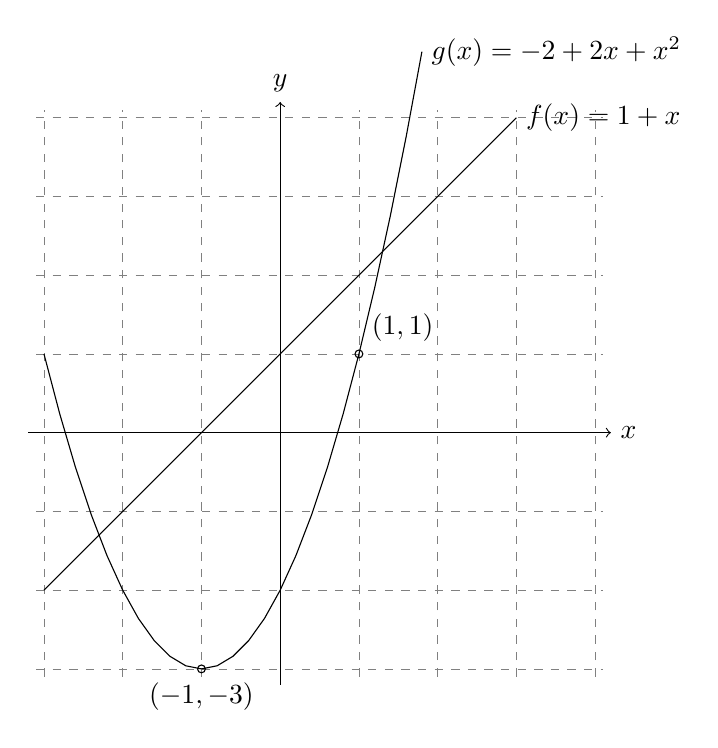
\begin{tikzpicture}
        \draw[very thin,color=gray,dashed] (-3.1,-3.1) grid (4.1,4.1);

        \node[draw,circle,radius=1pt,inner sep=1pt,black,label={45:$(1, 1)$}] at (1,1) {};
        \node[draw,circle,radius=1pt,inner sep=1pt,black,label={270:$(-1, -3)$}] at (-1,-3) {};

        \draw[->] (-3.2,0) -- (4.2,0) node[right] {$x$};
        \draw[->] (0,-3.2) -- (0,4.2) node[above] {$y$};

        \draw[domain=-3:3]    plot (\x,{1+\x})             node[right] {$f(x) = 1+x$};
        \draw[domain=-3:1.8]   plot (\x,{-2+2*\x+\x*\x})    node[right] {$g(x) = -2+2x+x^{2}$};
    \end{tikzpicture}
    \caption{Một phần đồ thị của hai hàm số $x\mapsto 1+x$ và $x\mapsto -2+2x+x^{2}$ trong mặt phẳng tọa độ Descartes.}\label{fig:graph-of-linear-function-and-quadratic-function}
\end{figure}

Chúng ta quan sát Hình~\ref{fig:graph-of-linear-function-and-quadratic-function}. Đồ thị hàm số $x\mapsto -2 + 2x + x^{2}$ đi qua điểm $(-1, 3)$ và $(1, 1)$. Bên cạnh đó, thuần túy bằng quan sát, chúng ta có thể thấy rằng với mọi số thực $a$ thuộc khoảng mở $(1, 3)$ (hay $(g(-1), g(1))$), tồn tại số thực $c$ thuộc khoảng mở $(-1, 1)$ sao cho $g(c) = a$. Điều tương tự cũng đúng với hàm số $x\mapsto 1 + x$. Hiện tượng này vẫn đúng với hàm số liên tục trên một khoảng đóng, và được phát biểu thành định lý sau.

\begin{theorem}[Định lý giá trị trung gian\index{Định lý giá trị trung gian}]
    Nếu hàm thực $f$ liên tục trên khoảng đóng $[a, b]$ với $a < b$ và $f(a)\ne f(b)$ thì với mỗi số thực $v$ thuộc khoảng mở $( \min\{ f(a), f(b) \}, \max\{ f(a), f(b) \} )$, tồn tại số thực $c$ thuộc khoảng mở $(a, b)$ sao cho $f(c) = v$.
\end{theorem}

Chứng minh dưới đây có trong cuốn sách Mathematical Analysis I của tác giả Zorich~\cite{zorich}, với cách tiếp cận tương tự định lý Bolzano-Weierstra{\ss}.

\begin{proof}
    Nếu tồn tại số thực $c$ như vậy thì $c\ne a$ và $c\ne b$, vì $v\ne f(a)$ và $v\ne f(b)$.

    Chúng ta xét hàm thực $g: [a, b]\to \mathbb{R}$, $g(x) = f(x) - v$. Theo giả thiết, hàm $g$ nhận cả giá trị dương và âm trong khoảng đóng $[a, b]$. Chúng ta kí hiệu $a_{0} = a$, $b_{0} = b$, chia đổi khoảng này thành hai khoảng đóng $\left[a_{0}, \dfrac{1}{2}(a_{0}, b_{0})\right]$, $\left[\dfrac{1}{2}(a_{0} + b_{0}), b_{0}\right]$. Nếu $g$ nhận giá trị $0$ tại số thực ở chính giữa của khoảng đóng thì số thực đó là số thực cần tìm. Ngược lại, hàm $g$ nhận cả giá trị dương và âm trong ít nhất một trong hai khoảng đóng này --- Chúng ta kí hiệu khoảng đóng đó là $[a_{1}, b_{1}]$. Chúng ta tiếp tục quá trình trên với khoảng đóng $[a_{1}, b_{1}]$. Trong quá trình này, có hai khả năng.

    \begin{enumerate}[label={\textbf{Khả năng \arabic*.}},itemindent=1.5cm]
        \item Tồn tại số tự nhiên $n$ sao cho $g\left(\dfrac{1}{2}(a_{n} + b_{n})\right) = 0$.

              Khi đó, $\dfrac{1}{2}(a_{n} + b_{n})$ là số thực $c$ cần tìm.
        \item Không tồn tại số tự nhiên $n$ sao cho $g\left(\dfrac{1}{2}(a_{n} + b_{n})\right) = 0$.

              Theo định lý Cantor về các khoảng đóng lồng nhau, chúng ta suy ra $\bigcap_{n\in\mathbb{N}} [a_{n}, b_{n}]$ có phần tử duy nhất --- Chúng ta kí hiệu phần tử này là $c$.

              Theo cách xây dựng các khoảng đóng $[a_{n}, b_{n}]$, với mỗi số tự nhiên $n$, tồn tại các số thực $x_{n}$ và $y_{n}$ thuộc $[a_{n}, b_{n}]$ sao cho $g(x_{n}) < 0$ và $g(y_{n}) > 0$ (vì $g$ nhận cả giá trị dương và âm trong khoảng đóng $[a_{n}, b_{n}]$). Bên cạnh đó
              \[
                  \begin{split}
                      \abs{x_{n} - c} \leq \abs{a_{n} - b_{n}} = \frac{b_{0} - a_{0}}{2^{n}}\leq \frac{b_{0} - a_{0}}{n+1}, \\
                      \abs{y_{n} - c} \leq \abs{a_{n} - b_{n}} = \frac{b_{0} - a_{0}}{2^{n}}\leq \frac{b_{0} - a_{0}}{n+1}.
                  \end{split}
              \]

              Do đó, với mỗi số thực dương $\varepsilon$, với số tự nhiên $N = \floor{\dfrac{b_{0} - a_{0}}{\varepsilon}}$, với mọi số tự nhiên $n\geq N$, có $\abs{x_{n} - c} < \varepsilon$ và $\abs{y_{n} - c} < \varepsilon$. Theo định nghĩa giới hạn dãy số, ${(x_{n})}_{n\in\mathbb{N}}$ và ${(y_{n})}_{n\in\mathbb{N}}$ có giới hạn $c$.

              Theo Định lý~\ref{theorem:limits-of-functions-and-sequences}, chúng ta suy ra ${(g(x_{n}))}_{n\in\mathbb{N}}$ và ${(g(y_{n}))}_{n\in\mathbb{N}}$ có giới hạn $g(c)$. Vì $g(x_{n}) < 0$ và $g(y_{n}) > 0$ với mọi số tự nhiên $n$ nên theo Định lý~\ref{theorem:order-of-convergent-sequences}, chúng ta suy ra $g(c)\leq 0$ và $g(c)\geq 0$. Do đó $g(c) = 0$.
    \end{enumerate}

    Vậy, tồn tại số thực $c$ trong khoảng mở $(a, b)$ sao cho $f(c) = v$.
\end{proof}

Định lý giá trị trung gian cung cấp một thuật toán xấp xỉ để tìm nghiệm gần đúng trong khoảng đóng $[a, b]$ của phương trình $f(x) = 0$ khi $f(a)f(b) < 0$, trong đó $f$ là hàm thực liên tục trên khoảng đóng $[a, b]$.

\begin{corollary}
    Cho hàm thực $f$ liên tục trên khoảng đóng $[a, b]$ với $a < b$ và $f(a)\ne f(b)$. Khi đó, nếu $f(a)f(b) < 0$ thì tồn tại số thực $c$ thuộc khoảng mở $(a, b)$ sao cho $f(c) = 0$.
\end{corollary}

\subsection{Hàm lũy thừa}

\begin{definition}[Lũy thừa với số mũ nguyên của số thực]
\end{definition}

\begin{theorem}[Căn bậc $n$]
\end{theorem}

\begin{definition}[Lũy thừa với số mũ hữu tỉ của số thực]
\end{definition}

\begin{theorem}
\end{theorem}

\begin{definition}[Lũy thừa với số mũ thực của số thực]
\end{definition}

\begin{theorem}
\end{theorem}

\begin{definition}[Hàm lũy thừa]
\end{definition}

\begin{theorem}
\end{theorem}

\subsection{Hàm mũ và hàm logarithm}

\begin{definition}[Hàm mũ]
\end{definition}

\begin{theorem}
\end{theorem}

\begin{definition}[Hàm logarithm]
\end{definition}

\begin{theorem}
\end{theorem}


